% =========================================================================
% CVPR 2027 Submission — "CropCode: Inverse Procedural Modeling of Occluded Row Crop Geometry from Sparse Multimodal Field Observations"
% =========================================================================
\documentclass[10pt,twocolumn,letterpaper]{article}

%%%%%%%%% PAPER TYPE  - PLEASE UPDATE FOR FINAL VERSION
\usepackage[review]{cvpr}      % To produce the REVIEW version
% \usepackage{cvpr}              % To produce the CAMERA-READY version
% \usepackage[pagenumbers]{cvpr} % To force page numbers, e.g. for an arXiv version
% Chart colors (labmate, 2026-11-10: supplement ablation charts)
\definecolor{seriesF}{HTML}{2A78D6}
\definecolor{seriesP}{HTML}{1BAF7A}
\definecolor{seriesR}{HTML}{4A3AA7}
\definecolor{gridc}{HTML}{E4E3DF}
\definecolor{axisc}{HTML}{52514E}
\usepackage{tikz}
\usepackage{pgfplots}
\pgfplotsset{compat=1.18}
\usetikzlibrary{arrows.meta}
% Contact-solver pseudocode (supplement, Dataset Generation Details)
\usepackage{algorithm}
\usepackage[noend]{algpseudocode}
\algrenewcommand\algorithmiccomment[1]{\hfill{\footnotesize\textcolor{black!60}{$\triangleright$ #1}}}
\newcommand{\Meets}{\textsc{Meets}}

% Import additional packages in the preamble file, before hyperref
%%%%%%%%%%%%%%%%%%%%%%%%%%%%%%%%%%%%%%%%%%%%%%%%%%%%%%%%%%%%%%%%%%%%%%%%%%%
% ==== preamble.tex (inlined) ====
%%%%%%%%%%%%%%%%%%%%%%%%%%%%%%%%%%%%%%%%%%%%%%%%%%%%%%%%%%%%%%%%%%%%%%%%%%%
%% This file contains a number of tweaks that are typically applied to the main document.
%% They are not enabled by default, but can be enabled by uncommenting the relevant lines.

%%
%% Inline annotations; for predefined colors, refer to "dvipsnames" in the xcolor package:
%% https://tinyurl.com/overleaf-colors
%%
\newcommand{\red}[1]{{\color{red}#1}}
\newcommand{\todo}[1]{{\color{red}#1}}
\newcommand{\TODO}[1]{\textbf{\color{red}[TODO: #1]}}
%%
%% disable for camera ready / submission by uncommenting these lines  
%%
% \renewcommand{\TODO}[1]{}
% \renewcommand{\todo}[1]{#1}

%%
%% work harder in optimizing text layout. Typically shrinks text by 1/6 of page, enable
%% it at the very end of the writing process, when you are just above the page limit
%%
\usepackage{microtype}

%%
%% fine-tune paragraph spacing
%%
% \renewcommand{\paragraph}[1]{\vspace{.5em}\noindent\textbf{#1.}}

%%
%% globally adjusts space between figure and caption
%%
% \setlength{\abovecaptionskip}{.5em}

%%
%% Allows "the use of \paper to refer to the project name"
%% with automatic management of space at the end of the word
%%
% \usepackage{xspace}
% \newcommand{\paper}{ProjectName\xspace}

%%
%% Commonly used math definitions
%%
% \DeclareMathOperator*{\argmin}{arg\,min}
% \DeclareMathOperator*{\argmax}{arg\,max}

%%
%% Tigthen underline
%%
% \usepackage{soul}
% \setuldepth{foobar}
%% Allow a double-column top float to fill nearly the whole page (tall figure* floats such as
%% fig:rowsex, 5.3 in, stay next to their section; [p] double floats flush only at \clearpage).
\renewcommand{\dbltopfraction}{0.99}

%% Revision marking: text changed or added after the 2026-11-05 shared draft is
%% set in blue. For the submission, switch to the no-op definition below.
\newcommand{\upd}[1]{{\color{blue}#1}}
% \renewcommand{\upd}[1]{#1}
% Edits made from 2026-11-07 on (after the blue pass) are purple; a macro name cannot contain a digit, so \upd2 is \updtwo.
\newcommand{\updtwo}[1]{{\color{purple}#1}}
% \renewcommand{\updtwo}[1]{#1}
%%%%%%%%%%%%%%%%%%%%%%%%%%%%%%%%%%%%%%%%%%%%%%%%%%%%%%%%%%%%%%%%%%%%%%%%%%%
% ==== end preamble.tex ====
%%%%%%%%%%%%%%%%%%%%%%%%%%%%%%%%%%%%%%%%%%%%%%%%%%%%%%%%%%%%%%%%%%%%%%%%%%%

% It is strongly recommended to use hyperref, especially for the review version.
\definecolor{cvprblue}{rgb}{0.21,0.49,0.74}
\usepackage[pagebackref,breaklinks,colorlinks,allcolors=cvprblue]{hyperref}

% ---- Method & Dataset Name Macros ----------------------------------------
\newcommand{\method}{\textsc{CropCode}}
\newcommand{\dataset}{\textsc{FieldScan}}
\providecommand{\CropCode}{\textsc{CropCode}}
\providecommand{\FieldProc}{\textsc{FieldScan}}

% ---- Helper Macros --------------------------------------------------------
% \todo is defined in preamble.tex; \providecommand keeps this line a no-op.
\providecommand{\todo}[1]{\textcolor{red}{#1}}
\newcommand{\oldnum}[1]{\textcolor{purple}{#1}}
\newcommand{\cmark}{\checkmark}
\newcommand{\xmark}{$\times$}
\providecommand{\R}{\mathbb{R}}

%%%%%%%%% PAPER ID & METADATA
\def\paperID{28592} % CVPR 2027 submission number
\def\confName{CVPR}
\def\confYear{2027}

% ---- Title --------------------------------------------------------------
\title{CropCode: Inverse Procedural Modeling of Occluded Row Crop Geometry from Sparse Multimodal Field Observations}

% ---- Keywords (for the submission form; CVPR PDFs do not print keywords) ----
% inverse procedural modeling; plant phenotyping; multimodal masked autoencoders;
% cross-modal distillation; point cloud reconstruction; occlusion;
% synthetic data pretraining; digital agriculture
% Subject areas: 3D from multi-view and sensors (primary);
% self-supervised representation learning; datasets and benchmarks;
% vision applications and systems (agriculture)

% Double-blind review author block
\author{Anonymous CVPR submission\\
Paper ID \paperID}

\date{}

\begin{document}

% Chart style
\pgfplotsset{
  abl/.style={
    width=\columnwidth,
    height=4.4cm,
    axis x line*=bottom,
    axis y line*=left,
    axis line style={axisc},
    tick style={axisc, line width=0.4pt},
    ymajorgrids,
    grid style={gridc, line width=0.4pt},
    tick label style={font=\footnotesize},
    label style={font=\footnotesize},
    legend style={
      font=\footnotesize,
      draw=none,
      fill=none,
      at={(0.5,1.03)},
      anchor=south,
      legend columns=3,
      /tikz/every even column/.append style={column sep=8pt}
    },
  },
}

% Title and teaser share the one-column head of page 1
\twocolumn[{%
\renewcommand\twocolumn[1][]{#1}%
\maketitle
\begin{center}%
  \resizebox{\textwidth}{!}{% Fig. 1 teaser, UGG-idea variant, WIDE layout (2026-11-13; user: "try to make it wider so that it will take less
% space"). One row instead of two: the two row photographs (sorghum, maize) -> the model -> the two centre plants'
% procedural parameters. At \textwidth it is ~40 % of the two-row version's height; type sizes raised so the printed
% sizes match the two-row version. Not used by main.tex (which inputs Figures/fig_teaser_tikz).
% Conventions from the UGG paper (Unified Generative Geometry Model): one pastel colour per stream (image blue,
% parameters purple), inputs in dashed rounded boxes, outputs solid, a model block with a soft gradient through the
% stream colours and a dashed rule, one grey frame around what the model writes, grey block arrows. Font: \sffamily
% (Helvetica under the cvpr/times package), as the paper's teaser.
% Content (user, 2026-11-13): header "Model"; the output is the procedural parameters only, drawn as in the
% any-to-all figure (figures/make_teaser_recipe_tiles.py: the written recipe in purple over the true one in grey),
% no value text. Plants: the held-out test rows of figures/make_teaser_v2.py --mode row (Sorghum_10113, plant_0106).
% Include with \resizebox{\textwidth}{!}{% Fig. 1 teaser, UGG-idea variant, WIDE layout (2026-11-13; user: "try to make it wider so that it will take less
% space"). One row instead of two: the two row photographs (sorghum, maize) -> the model -> the two centre plants'
% procedural parameters. At \textwidth it is ~40 % of the two-row version's height; type sizes raised so the printed
% sizes match the two-row version. Not used by main.tex (which inputs Figures/fig_teaser_tikz).
% Conventions from the UGG paper (Unified Generative Geometry Model): one pastel colour per stream (image blue,
% parameters purple), inputs in dashed rounded boxes, outputs solid, a model block with a soft gradient through the
% stream colours and a dashed rule, one grey frame around what the model writes, grey block arrows. Font: \sffamily
% (Helvetica under the cvpr/times package), as the paper's teaser.
% Content (user, 2026-11-13): header "Model"; the output is the procedural parameters only, drawn as in the
% any-to-all figure (figures/make_teaser_recipe_tiles.py: the written recipe in purple over the true one in grey),
% no value text. Plants: the held-out test rows of figures/make_teaser_v2.py --mode row (Sorghum_10113, plant_0106).
% Include with \resizebox{\textwidth}{!}{% Fig. 1 teaser, UGG-idea variant, WIDE layout (2026-11-13; user: "try to make it wider so that it will take less
% space"). One row instead of two: the two row photographs (sorghum, maize) -> the model -> the two centre plants'
% procedural parameters. At \textwidth it is ~40 % of the two-row version's height; type sizes raised so the printed
% sizes match the two-row version. Not used by main.tex (which inputs Figures/fig_teaser_tikz).
% Conventions from the UGG paper (Unified Generative Geometry Model): one pastel colour per stream (image blue,
% parameters purple), inputs in dashed rounded boxes, outputs solid, a model block with a soft gradient through the
% stream colours and a dashed rule, one grey frame around what the model writes, grey block arrows. Font: \sffamily
% (Helvetica under the cvpr/times package), as the paper's teaser.
% Content (user, 2026-11-13): header "Model"; the output is the procedural parameters only, drawn as in the
% any-to-all figure (figures/make_teaser_recipe_tiles.py: the written recipe in purple over the true one in grey),
% no value text. Plants: the held-out test rows of figures/make_teaser_v2.py --mode row (Sorghum_10113, plant_0106).
% Include with \resizebox{\textwidth}{!}{\input{Figures/fig_teaser_tikz_ugg}} (needs \usetikzlibrary{arrows.meta}).
\definecolor{tInk}{HTML}{1D221C}\definecolor{tMuted}{HTML}{5F685C}%
\definecolor{uRgbE}{HTML}{809EC2}\definecolor{uRgbF}{HTML}{E6ECF3}\definecolor{uRgbI}{HTML}{3F5F8F}%
\definecolor{uPcF}{HTML}{F6E9ED}\definecolor{uDepF}{HTML}{FAF2D4}%
\definecolor{uTxE}{HTML}{9D8CC4}\definecolor{uTxF}{HTML}{EAE7F2}\definecolor{uTxI}{HTML}{5E4A96}%
\definecolor{uOutE}{HTML}{B4B4B8}\definecolor{uArrow}{HTML}{8C8C8C}\definecolor{uModE}{HTML}{9A9A9A}%
\pgfdeclarehorizontalshading{uggband}{100bp}{color(0bp)=(uRgbF); color(30bp)=(uRgbF); color(45bp)=(uDepF); color(60bp)=(uPcF); color(75bp)=(uTxF); color(100bp)=(uTxF)}%
\begin{tikzpicture}[x=0.005in, y=-0.005in]
\useasboundingbox (0,0) rectangle (1320,340);
\tikzset{hdr/.style={anchor=center, inner sep=0, align=center, font={\fontsize{8.5}{10.2}\selectfont\sffamily\bfseries}},
         sp/.style={anchor=base, inner sep=0, align=center, text=tInk, font={\fontsize{7.2}{8.6}\selectfont\sffamily\bfseries}},
         tcap/.style={anchor=north, inner sep=0, align=center, text=tMuted, font={\fontsize{5.6}{6.8}\selectfont\sffamily}},
         blk/.style={color=uArrow, line width=3.0pt, -{Triangle[length=5.5pt,width=8.5pt]}}}
% ---- headers ----
\node[hdr, text=uRgbI] at (260.0,18.0) {Image of an occluded crop row (input)};
\node[hdr, text=tInk] at (662.0,18.0) {Model};
\node[hdr, text=uTxI] at (1055.0,18.0) {Procedural parameters of the center plant};
% ---- inputs: the row photographs ----
\node[sp] at (136.0,56.0) {sorghum};
\node[sp] at (384.0,56.0) {maize};
\draw[draw=uRgbE, line width=1.0pt, rounded corners=6.5pt, fill=uRgbF, dash pattern=on 3pt off 2pt] (20.0,68.0) rectangle (252.0,300.0);
\node[anchor=north west, inner sep=0] at (26.0,74.0) {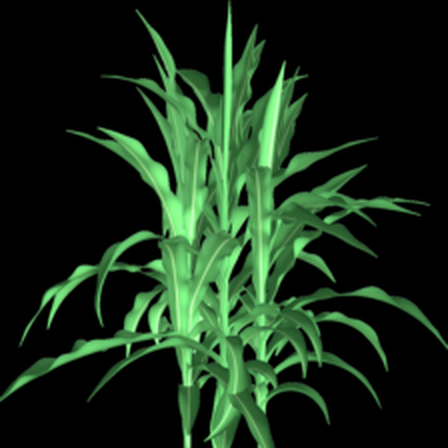
\includegraphics[width=1.1000in, height=1.1000in]{Figures/teaser/s_rgb.png}};
\draw[draw=white, densely dashed, line width=0.80pt] (104.0,88.0) rectangle (168.0,284.0);
\node[anchor=north west, inner sep=1.5pt, text=white, font={\fontsize{5.0}{6.0}\selectfont\sffamily\bfseries}] at (104.0,88.0) {target plant};
\node[tcap] at (136.0,308.0) {25\,\% hidden by neighbours};
\draw[draw=uRgbE, line width=1.0pt, rounded corners=6.5pt, fill=uRgbF, dash pattern=on 3pt off 2pt] (268.0,68.0) rectangle (500.0,300.0);
\node[anchor=north west, inner sep=0] at (274.0,74.0) {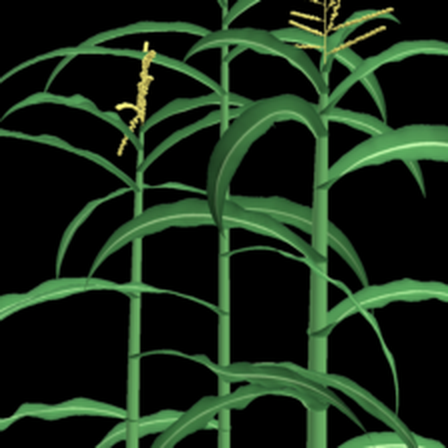
\includegraphics[width=1.1000in, height=1.1000in]{Figures/teaser/m_rgb.png}};
\draw[draw=white, densely dashed, line width=0.80pt] (354.0,84.0) rectangle (430.0,290.0);
\node[anchor=north west, inner sep=1.5pt, text=white, font={\fontsize{4.6}{5.6}\selectfont\sffamily\bfseries}] at (354.0,84.0) {target plant};
\node[tcap] at (384.0,308.0) {22\,\% hidden by neighbours};
\draw[blk] (510.0,184.0) -- (566.0,184.0);
% ---- the model ----
\draw[draw=uModE, line width=1.0pt, rounded corners=8.6pt, shading=uggband, shading angle=0] (574.0,68.0) rectangle (750.0,300.0);
\node[anchor=center, inner sep=0, text=tInk, font={\fontsize{9.0}{10.8}\selectfont\sffamily\bfseries}] at (662.0,120.0) {CropCode};
\draw[draw=uModE, line width=0.6pt, dash pattern=on 2.2pt off 1.6pt] (600.0,146.0) -- (724.0,146.0);
\node[anchor=north, inner sep=0, align=center, text=tInk, font={\fontsize{5.3}{6.6}\selectfont\sffamily}] at (662.0,166.0) {any-to-any\\autoencoder over\\photographs, depth,\\clouds and recipes;\\pretrained on single\\plants, fine-tuned\\on crop rows};
\draw[blk] (758.0,184.0) -- (806.0,184.0);
% ---- outputs: the procedural parameters ----
\draw[draw=uOutE, line width=0.9pt, rounded corners=8.6pt] (814.0,34.0) rectangle (1302.0,334.0);
\node[sp] at (938.0,56.0) {sorghum};
\node[sp] at (1178.0,56.0) {maize};
\draw[draw=uTxE, line width=1.0pt, rounded corners=6.5pt, fill=uTxF] (822.0,68.0) rectangle (1054.0,300.0);
\node[anchor=north west, inner sep=0] at (828.0,74.0) {
\includegraphics[width=1.1000in, height=1.1000in]{Figures/teaser/s_recipe.png}};
\draw[draw=uTxE, line width=1.0pt, rounded corners=6.5pt, fill=uTxF] (1062.0,68.0) rectangle (1294.0,300.0);
\node[anchor=north west, inner sep=0] at (1068.0,74.0) {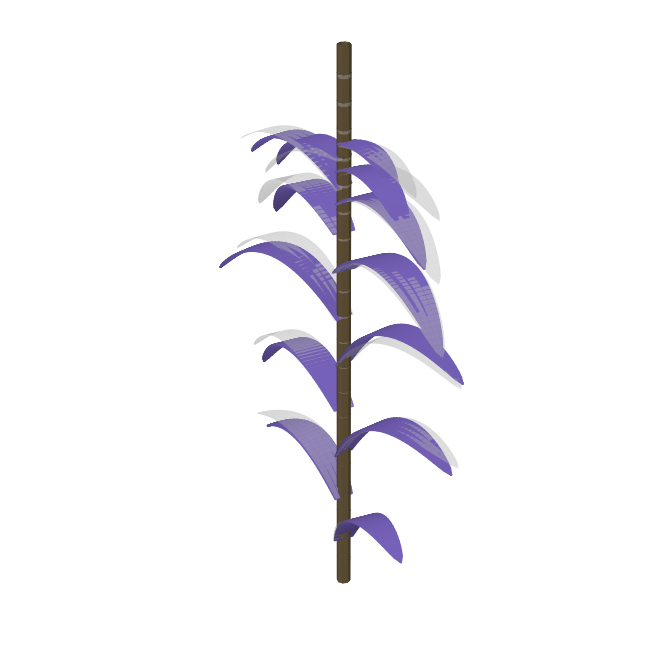
\includegraphics[width=1.1000in, height=1.1000in]{Figures/teaser/m_recipe.png}};
\node[tcap] at (1058.0,308.0) {\textcolor{uTxI}{\textbf{purple}: written by CropCode}\quad grey: the true plant};
\end{tikzpicture}
} (needs \usetikzlibrary{arrows.meta}).
\definecolor{tInk}{HTML}{1D221C}\definecolor{tMuted}{HTML}{5F685C}%
\definecolor{uRgbE}{HTML}{809EC2}\definecolor{uRgbF}{HTML}{E6ECF3}\definecolor{uRgbI}{HTML}{3F5F8F}%
\definecolor{uPcF}{HTML}{F6E9ED}\definecolor{uDepF}{HTML}{FAF2D4}%
\definecolor{uTxE}{HTML}{9D8CC4}\definecolor{uTxF}{HTML}{EAE7F2}\definecolor{uTxI}{HTML}{5E4A96}%
\definecolor{uOutE}{HTML}{B4B4B8}\definecolor{uArrow}{HTML}{8C8C8C}\definecolor{uModE}{HTML}{9A9A9A}%
\pgfdeclarehorizontalshading{uggband}{100bp}{color(0bp)=(uRgbF); color(30bp)=(uRgbF); color(45bp)=(uDepF); color(60bp)=(uPcF); color(75bp)=(uTxF); color(100bp)=(uTxF)}%
\begin{tikzpicture}[x=0.005in, y=-0.005in]
\useasboundingbox (0,0) rectangle (1320,340);
\tikzset{hdr/.style={anchor=center, inner sep=0, align=center, font={\fontsize{8.5}{10.2}\selectfont\sffamily\bfseries}},
         sp/.style={anchor=base, inner sep=0, align=center, text=tInk, font={\fontsize{7.2}{8.6}\selectfont\sffamily\bfseries}},
         tcap/.style={anchor=north, inner sep=0, align=center, text=tMuted, font={\fontsize{5.6}{6.8}\selectfont\sffamily}},
         blk/.style={color=uArrow, line width=3.0pt, -{Triangle[length=5.5pt,width=8.5pt]}}}
% ---- headers ----
\node[hdr, text=uRgbI] at (260.0,18.0) {Image of an occluded crop row (input)};
\node[hdr, text=tInk] at (662.0,18.0) {Model};
\node[hdr, text=uTxI] at (1055.0,18.0) {Procedural parameters of the center plant};
% ---- inputs: the row photographs ----
\node[sp] at (136.0,56.0) {sorghum};
\node[sp] at (384.0,56.0) {maize};
\draw[draw=uRgbE, line width=1.0pt, rounded corners=6.5pt, fill=uRgbF, dash pattern=on 3pt off 2pt] (20.0,68.0) rectangle (252.0,300.0);
\node[anchor=north west, inner sep=0] at (26.0,74.0) {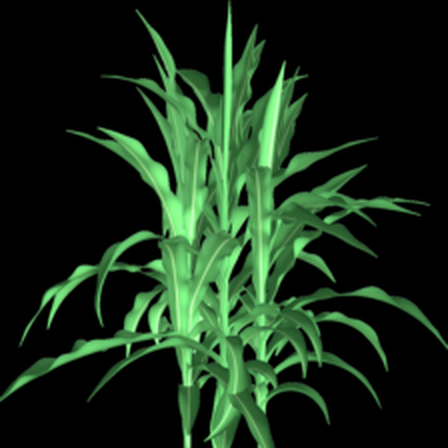
\includegraphics[width=1.1000in, height=1.1000in]{Figures/teaser/s_rgb.png}};
\draw[draw=white, densely dashed, line width=0.80pt] (104.0,88.0) rectangle (168.0,284.0);
\node[anchor=north west, inner sep=1.5pt, text=white, font={\fontsize{5.0}{6.0}\selectfont\sffamily\bfseries}] at (104.0,88.0) {target plant};
\node[tcap] at (136.0,308.0) {25\,\% hidden by neighbours};
\draw[draw=uRgbE, line width=1.0pt, rounded corners=6.5pt, fill=uRgbF, dash pattern=on 3pt off 2pt] (268.0,68.0) rectangle (500.0,300.0);
\node[anchor=north west, inner sep=0] at (274.0,74.0) {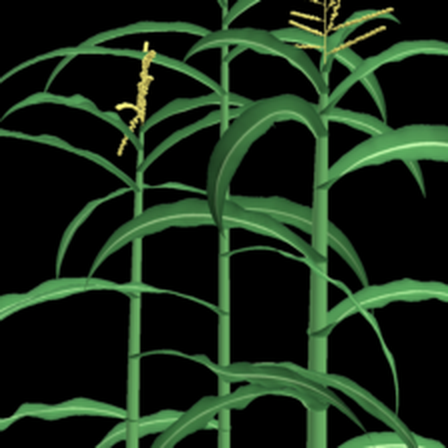
\includegraphics[width=1.1000in, height=1.1000in]{Figures/teaser/m_rgb.png}};
\draw[draw=white, densely dashed, line width=0.80pt] (354.0,84.0) rectangle (430.0,290.0);
\node[anchor=north west, inner sep=1.5pt, text=white, font={\fontsize{4.6}{5.6}\selectfont\sffamily\bfseries}] at (354.0,84.0) {target plant};
\node[tcap] at (384.0,308.0) {22\,\% hidden by neighbours};
\draw[blk] (510.0,184.0) -- (566.0,184.0);
% ---- the model ----
\draw[draw=uModE, line width=1.0pt, rounded corners=8.6pt, shading=uggband, shading angle=0] (574.0,68.0) rectangle (750.0,300.0);
\node[anchor=center, inner sep=0, text=tInk, font={\fontsize{9.0}{10.8}\selectfont\sffamily\bfseries}] at (662.0,120.0) {CropCode};
\draw[draw=uModE, line width=0.6pt, dash pattern=on 2.2pt off 1.6pt] (600.0,146.0) -- (724.0,146.0);
\node[anchor=north, inner sep=0, align=center, text=tInk, font={\fontsize{5.3}{6.6}\selectfont\sffamily}] at (662.0,166.0) {any-to-any\\autoencoder over\\photographs, depth,\\clouds and recipes;\\pretrained on single\\plants, fine-tuned\\on crop rows};
\draw[blk] (758.0,184.0) -- (806.0,184.0);
% ---- outputs: the procedural parameters ----
\draw[draw=uOutE, line width=0.9pt, rounded corners=8.6pt] (814.0,34.0) rectangle (1302.0,334.0);
\node[sp] at (938.0,56.0) {sorghum};
\node[sp] at (1178.0,56.0) {maize};
\draw[draw=uTxE, line width=1.0pt, rounded corners=6.5pt, fill=uTxF] (822.0,68.0) rectangle (1054.0,300.0);
\node[anchor=north west, inner sep=0] at (828.0,74.0) {
\includegraphics[width=1.1000in, height=1.1000in]{Figures/teaser/s_recipe.png}};
\draw[draw=uTxE, line width=1.0pt, rounded corners=6.5pt, fill=uTxF] (1062.0,68.0) rectangle (1294.0,300.0);
\node[anchor=north west, inner sep=0] at (1068.0,74.0) {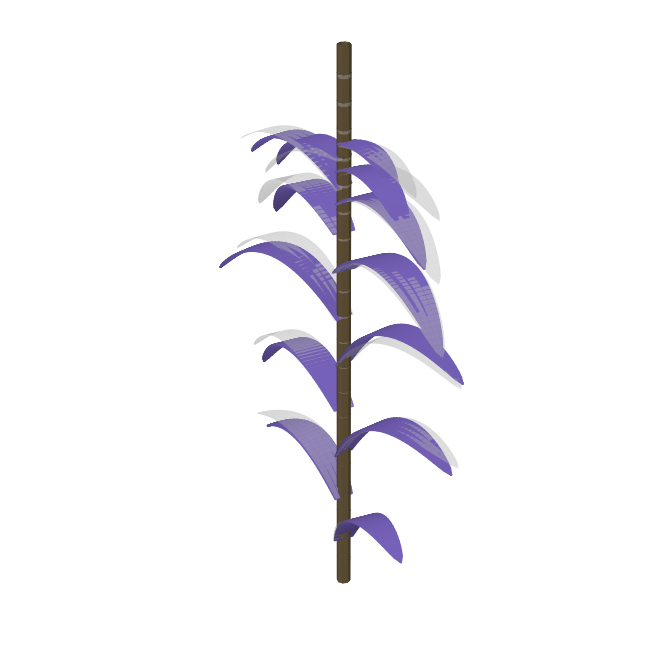
\includegraphics[width=1.1000in, height=1.1000in]{Figures/teaser/m_recipe.png}};
\node[tcap] at (1058.0,308.0) {\textcolor{uTxI}{\textbf{purple}: written by CropCode}\quad grey: the true plant};
\end{tikzpicture}
} (needs \usetikzlibrary{arrows.meta}).
\definecolor{tInk}{HTML}{1D221C}\definecolor{tMuted}{HTML}{5F685C}%
\definecolor{uRgbE}{HTML}{809EC2}\definecolor{uRgbF}{HTML}{E6ECF3}\definecolor{uRgbI}{HTML}{3F5F8F}%
\definecolor{uPcF}{HTML}{F6E9ED}\definecolor{uDepF}{HTML}{FAF2D4}%
\definecolor{uTxE}{HTML}{9D8CC4}\definecolor{uTxF}{HTML}{EAE7F2}\definecolor{uTxI}{HTML}{5E4A96}%
\definecolor{uOutE}{HTML}{B4B4B8}\definecolor{uArrow}{HTML}{8C8C8C}\definecolor{uModE}{HTML}{9A9A9A}%
\pgfdeclarehorizontalshading{uggband}{100bp}{color(0bp)=(uRgbF); color(30bp)=(uRgbF); color(45bp)=(uDepF); color(60bp)=(uPcF); color(75bp)=(uTxF); color(100bp)=(uTxF)}%
\begin{tikzpicture}[x=0.005in, y=-0.005in]
\useasboundingbox (0,0) rectangle (1320,340);
\tikzset{hdr/.style={anchor=center, inner sep=0, align=center, font={\fontsize{8.5}{10.2}\selectfont\sffamily\bfseries}},
         sp/.style={anchor=base, inner sep=0, align=center, text=tInk, font={\fontsize{7.2}{8.6}\selectfont\sffamily\bfseries}},
         tcap/.style={anchor=north, inner sep=0, align=center, text=tMuted, font={\fontsize{5.6}{6.8}\selectfont\sffamily}},
         blk/.style={color=uArrow, line width=3.0pt, -{Triangle[length=5.5pt,width=8.5pt]}}}
% ---- headers ----
\node[hdr, text=uRgbI] at (260.0,18.0) {Image of an occluded crop row (input)};
\node[hdr, text=tInk] at (662.0,18.0) {Model};
\node[hdr, text=uTxI] at (1055.0,18.0) {Procedural parameters of the center plant};
% ---- inputs: the row photographs ----
\node[sp] at (136.0,56.0) {sorghum};
\node[sp] at (384.0,56.0) {maize};
\draw[draw=uRgbE, line width=1.0pt, rounded corners=6.5pt, fill=uRgbF, dash pattern=on 3pt off 2pt] (20.0,68.0) rectangle (252.0,300.0);
\node[anchor=north west, inner sep=0] at (26.0,74.0) {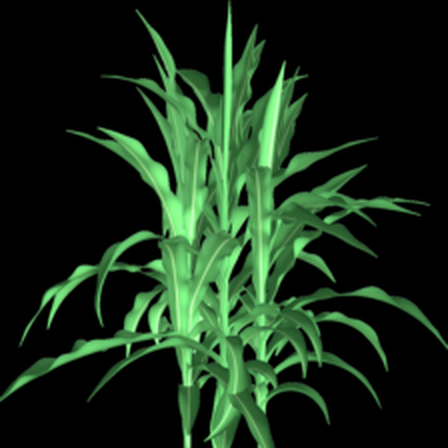
\includegraphics[width=1.1000in, height=1.1000in]{Figures/teaser/s_rgb.png}};
\draw[draw=white, densely dashed, line width=0.80pt] (104.0,88.0) rectangle (168.0,284.0);
\node[anchor=north west, inner sep=1.5pt, text=white, font={\fontsize{5.0}{6.0}\selectfont\sffamily\bfseries}] at (104.0,88.0) {target plant};
\node[tcap] at (136.0,308.0) {25\,\% hidden by neighbours};
\draw[draw=uRgbE, line width=1.0pt, rounded corners=6.5pt, fill=uRgbF, dash pattern=on 3pt off 2pt] (268.0,68.0) rectangle (500.0,300.0);
\node[anchor=north west, inner sep=0] at (274.0,74.0) {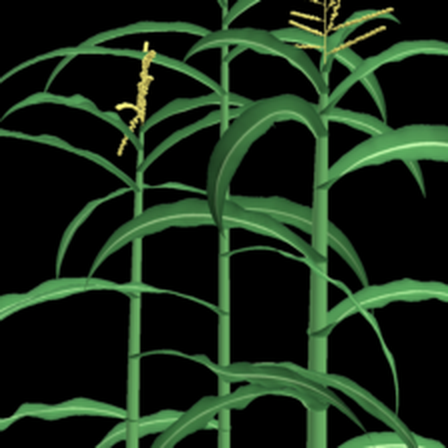
\includegraphics[width=1.1000in, height=1.1000in]{Figures/teaser/m_rgb.png}};
\draw[draw=white, densely dashed, line width=0.80pt] (354.0,84.0) rectangle (430.0,290.0);
\node[anchor=north west, inner sep=1.5pt, text=white, font={\fontsize{4.6}{5.6}\selectfont\sffamily\bfseries}] at (354.0,84.0) {target plant};
\node[tcap] at (384.0,308.0) {22\,\% hidden by neighbours};
\draw[blk] (510.0,184.0) -- (566.0,184.0);
% ---- the model ----
\draw[draw=uModE, line width=1.0pt, rounded corners=8.6pt, shading=uggband, shading angle=0] (574.0,68.0) rectangle (750.0,300.0);
\node[anchor=center, inner sep=0, text=tInk, font={\fontsize{9.0}{10.8}\selectfont\sffamily\bfseries}] at (662.0,120.0) {CropCode};
\draw[draw=uModE, line width=0.6pt, dash pattern=on 2.2pt off 1.6pt] (600.0,146.0) -- (724.0,146.0);
\node[anchor=north, inner sep=0, align=center, text=tInk, font={\fontsize{5.3}{6.6}\selectfont\sffamily}] at (662.0,166.0) {any-to-any\\autoencoder over\\photographs, depth,\\clouds and recipes;\\pretrained on single\\plants, fine-tuned\\on crop rows};
\draw[blk] (758.0,184.0) -- (806.0,184.0);
% ---- outputs: the procedural parameters ----
\draw[draw=uOutE, line width=0.9pt, rounded corners=8.6pt] (814.0,34.0) rectangle (1302.0,334.0);
\node[sp] at (938.0,56.0) {sorghum};
\node[sp] at (1178.0,56.0) {maize};
\draw[draw=uTxE, line width=1.0pt, rounded corners=6.5pt, fill=uTxF] (822.0,68.0) rectangle (1054.0,300.0);
\node[anchor=north west, inner sep=0] at (828.0,74.0) {
\includegraphics[width=1.1000in, height=1.1000in]{Figures/teaser/s_recipe.png}};
\draw[draw=uTxE, line width=1.0pt, rounded corners=6.5pt, fill=uTxF] (1062.0,68.0) rectangle (1294.0,300.0);
\node[anchor=north west, inner sep=0] at (1068.0,74.0) {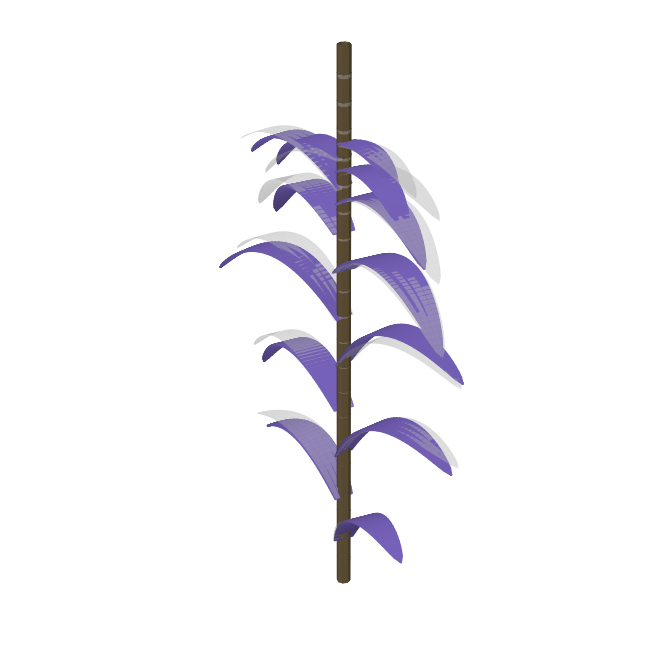
\includegraphics[width=1.1000in, height=1.1000in]{Figures/teaser/m_recipe.png}};
\node[tcap] at (1058.0,308.0) {\textcolor{uTxI}{\textbf{purple}: written by CropCode}\quad grey: the true plant};
\end{tikzpicture}
}%
  \captionof{figure}{\textbf{Any sensor in, procedural plant out.} From any subset of field-practical modalities (a single photograph, a depth frame, or a point cloud truncated by row neighbors), \method{} recovers the full procedural representation of the plant: a kilobyte-scale, physiologically interpretable parameter set that can be re-rendered to complete geometry, used as simulation input, and used for trait analytics at field scale. Shown: one held-out simulated test row per species, seen broadside by the rover camera. The dashed box marks the target plant for the reader; the model receives no marking. The model fine-tuned on rows reads the photograph of the row (a depth frame or point cloud serves equally) and writes the target plant's procedural parameters, drawn as a stem with each leaf at its insertion height, length, width and side: purple is the recipe the model writes, grey the true recipe. The written height is within 2\,\% of the true height for both plants, and the leaf count within one leaf (Regime III, Sec.~\ref{sec:regime3}).}
  \label{fig:teaser}%
\end{center}%
\vspace{4pt}
}]

%%%%%%%%%%%%%%%%%%%%%%%%%%%%%%%%%%%%%%%%%%%%%%%%%%%%%%%%%%%%%%%%%%%%%%%%%%%
% ==== sec/0_abstract.tex (inlined) ====
%%%%%%%%%%%%%%%%%%%%%%%%%%%%%%%%%%%%%%%%%%%%%%%%%%%%%%%%%%%%%%%%%%%%%%%%%%%
\begin{abstract}
Editable, biologically interpretable 3D models of field-grown crops support
high-throughput phenotyping, \emph{in silico} breeding trials, and agronomic
digital twins, but recovering such models from field sensor data remains
difficult: plant organs are slender, neighboring plants occlude one another,
and a field campaign rarely yields more than a single photograph, a noisy
depth frame, or a partial point cloud per plant. Slender geometry under
occlusion is a regime in which learned 3D completion and Chamfer-based
evaluation both fail. In this work, we present \method{}, a multimodal
masked-autoencoder framework that recovers the complete procedural
representation of a plant, the generator parameters encoding leaf count,
insertion heights, blade angles, and surface geometry, from any subset of
RGB, depth, and point-cloud input in a single forward pass.
The model is pretrained on 15{,}000 procedurally generated plants per
species (maize and sorghum), fine-tuned on rows in which simulated neighbors
occlude the target, and distilled from a full-modality teacher into
single-sensor students.
Distillation lowers the cross-modal generation loss by 30\% in sorghum
and 44\% in maize, and halves the sorghum parameter error from a point cloud
alone.
Training on rows removes 92\% (maize) and 85\% (sorghum) of the error
that neighbors add for a model trained on isolated plants.
Controlled ablations in both species show that exposing most of the
procedural parameters to the encoder degrades phenotype recovery, while using
them only as a reconstruction target degrades the sorghum representation and
improves the maize one.
We further show that Chamfer distance and linear probes on the frozen
representation rank input modalities differently on slender geometry, and we
adopt the probe as the deciding metric.
On crop rows built from real plants of both species, accuracy
degrades zero-shot on plants taller than any training plant, and a brief
fine-tune on 75\% of the real plants brings the held-out rest to a 1.6\%
median height error and a leaf count within one leaf on 70\% of maize stops,
at milliseconds per plant against hours of manual specification or minutes
of staged-pipeline computation.
We will release \dataset{}, the 30{,}000-plant, two-species benchmark
behind these experiments, which pairs multimodal field captures under
simulated row occlusion with exact procedural ground truth.
\end{abstract}
%%%%%%%%%%%%%%%%%%%%%%%%%%%%%%%%%%%%%%%%%%%%%%%%%%%%%%%%%%%%%%%%%%%%%%%%%%%
% ==== end sec/0_abstract.tex ====
%%%%%%%%%%%%%%%%%%%%%%%%%%%%%%%%%%%%%%%%%%%%%%%%%%%%%%%%%%%%%%%%%%%%%%%%%%%
%%%%%%%%%%%%%%%%%%%%%%%%%%%%%%%%%%%%%%%%%%%%%%%%%%%%%%%%%%%%%%%%%%%%%%%%%%%
% ==== sec/1_intro.tex (inlined) ====
%%%%%%%%%%%%%%%%%%%%%%%%%%%%%%%%%%%%%%%%%%%%%%%%%%%%%%%%%%%%%%%%%%%%%%%%%%%
\section{Introduction}
\label{sec:intro}

% Fig. 1 (teaser) lives in the title block of main.tex, full width on page 1.

Accurate three-dimensional models of individual crop plants enable
high-throughput phenotyping of morphological traits such as leaf angle,
internode length, and canopy architecture, and they are the basis of emerging
agricultural digital twins in which breeding trials run \emph{in
silico}~\citep{hadadi2025procmaize, maizefield3d2025}. The representation
best suited to these uses is procedural: a compact set of biologically
interpretable parameters that a generator expands into complete, editable,
simulation-ready geometry~\citep{prusin1990abop, floraforge2026}.
A procedural plant occupies a few kilobytes where a laser scan occupies
megabytes, every parameter corresponds to a trait used by agronomists, and
the model can be edited, re-rendered, and perturbed in ways that unstructured
geometry does not support.
Field crops also instantiate a challenge of general interest in 3D
computer vision: recovering a parametric model of a thin, heavily occluded
object from partial multimodal observations.

Yet every existing route to procedural structure presupposes a
rich, clean observation: manual specification takes hours per
plant~\citep{floraforge2026}; a staged pipeline annotates laser scans with
a vision-language model and fits a descriptor to 5.4\,mm median accuracy,
but needs a complete scan of an isolated plant and about ten minutes per
plant~\citep{hadadi2026vlmmaize}; per-scene optimization searches generator
parameters against multi-view imagery~\citep{cropcraft2026}; and learned
models infer parametric plants only from a clean, complete point
cloud~\citep{demeter2025, ghrer2025paramplants}. A phenotyping campaign
produces the opposite: thousands of plants per day, each observed by
whichever sensor was practical. Crop plants are also slender (a maize blade
is centimeters wide, millimeters thick, up to a meter long) and occluded by
their row neighbors, whose leaves interleave with the target: in our field
simulations a third of the target's pixels and two thirds of the scene's
point cloud belong to neighbors. This regime breaks the assumptions of
learned 3D completion, whose benchmarks hold compact, largely convex
objects~\citep{yuan2018pcn,yu2021pointr}, and of Chamfer distance, which is
structurally insensitive to thin sheets~\citep{wu2021dcd, song2026structural};
occlusion-aware completion of plant organs outputs unstructured geometry
rather than structure~\citep{lee2026occ}. To our knowledge, no prior method
recovers a procedural, re-renderable representation of slender crop organs
from a single field-practical observation under row-neighbor occlusion.

\begin{figure*}[t]
  \centering
  \resizebox{\linewidth}{!}{% Generated by figures/_scene.py (Scene.render_tikz) for 'Fig 2 stages'; do not edit by hand, re-run the figure script.
% 6.875 x 4.42 in at 100 %; needs \usetikzlibrary{arrows.meta}; images in Figures/fig2/.
{%
\definecolor{c1D221C}{HTML}{1D221C}%
\definecolor{c2A9D8F}{HTML}{2A9D8F}%
\definecolor{c2B3A67}{HTML}{2B3A67}%
\definecolor{c30638E}{HTML}{30638E}%
\definecolor{c4A78B5}{HTML}{4A78B5}%
\definecolor{c5F685C}{HTML}{5F685C}%
\definecolor{c6AA84F}{HTML}{6AA84F}%
\definecolor{c888888}{HTML}{888888}%
\definecolor{c8A8A8A}{HTML}{8A8A8A}%
\definecolor{cB8860B}{HTML}{B8860B}%
\definecolor{cC0392B}{HTML}{C0392B}%
\definecolor{cD9E2F3}{HTML}{D9E2F3}%
\definecolor{cE0A82E}{HTML}{E0A82E}%
\definecolor{cEEF3FA}{HTML}{EEF3FA}%
\definecolor{cF1F8EE}{HTML}{F1F8EE}%
\definecolor{cF4F4F2}{HTML}{F4F4F2}%
\definecolor{cFBE3C4}{HTML}{FBE3C4}%
\definecolor{cFDF8EA}{HTML}{FDF8EA}%
\definecolor{cFFFFFF}{HTML}{FFFFFF}%
\begin{tikzpicture}[x=1in, y=1in]%
\useasboundingbox (0,0) rectangle (6.8750,4.4200);
\draw[draw=cE0A82E, line width=1.200pt, fill=cFDF8EA, rounded corners=0.0900in] (0.4000,2.7200) rectangle (4.9800,4.2800);
\draw[draw=cE0A82E, line width=0.900pt, fill=cFFFFFF, rounded corners=0.0500in] (0.5400,4.1700) rectangle (2.3858,4.3900);
\draw[draw=c6AA84F, line width=1.200pt, fill=cF1F8EE, rounded corners=0.0900in] (0.4000,1.4000) rectangle (4.9800,2.5600);
\draw[draw=c6AA84F, line width=0.900pt, fill=cFFFFFF, rounded corners=0.0500in] (0.5400,2.4500) rectangle (2.6363,2.6700);
\draw[draw=c4A78B5, line width=1.200pt, fill=cEEF3FA, rounded corners=0.0900in] (0.4000,0.0400) rectangle (4.9800,1.2400);
\draw[draw=c4A78B5, line width=0.900pt, fill=cFFFFFF, rounded corners=0.0500in] (0.5400,1.1300) rectangle (2.1352,1.3500);
\draw[draw=c2B3A67, line width=0.900pt, fill=cD9E2F3, line join=round] (2.6200,3.0300) -- (3.2923,3.2292) -- (3.2923,3.6608) -- (2.6200,3.8600) -- cycle;
\draw[draw=c2B3A67, line width=0.900pt, fill=cFBE3C4, line join=round] (3.3273,3.2458) -- (3.9000,3.1130) -- (3.9000,3.7770) -- (3.3273,3.6442) -- cycle;
\draw[draw=c888888, line width=0.900pt, fill=cFFFFFF, rounded corners=0.0500in] (0.5200,1.5500) rectangle (1.7700,2.2700);
\draw[draw=c2B3A67, line width=1.000pt, fill=cFFFFFF, rounded corners=0.0500in] (2.3000,1.5500) rectangle (3.5500,2.2700);
\draw[draw=c2B3A67, line width=0.900pt, fill=cD9E2F3, line join=round] (2.2300,0.4200) -- (2.8591,0.5256) -- (2.8591,0.7544) -- (2.2300,0.8600) -- cycle;
\draw[draw=c2B3A67, line width=0.900pt, fill=cFBE3C4, line join=round] (2.8941,0.5344) -- (3.4300,0.4640) -- (3.4300,0.8160) -- (2.8941,0.7456) -- cycle;
\draw[draw=c8A8A8A, line width=1.300pt, fill=cF4F4F2, rounded corners=0.0900in] (5.1000,0.0400) rectangle (6.8550,4.2800);
\draw[draw=cC0392B, line width=0.600pt, fill=cC0392B, rounded corners=0.0120in] (5.2400,3.6500) rectangle (5.3600,3.7700);
\draw[draw=cC0392B, line width=0.600pt, fill=cFFFFFF, rounded corners=0.0120in] (5.3950,3.6500) rectangle (5.5150,3.7700);
\draw[draw=cC0392B, line width=0.600pt, fill=cC0392B, rounded corners=0.0120in] (5.5500,3.6500) rectangle (5.6700,3.7700);
\draw[draw=cC0392B, line width=0.600pt, fill=cFFFFFF, rounded corners=0.0120in] (5.7050,3.6500) rectangle (5.8250,3.7700);
\draw[draw=cB8860B, line width=0.600pt, fill=cFFFFFF, rounded corners=0.0120in] (5.2400,3.3500) rectangle (5.3600,3.4700);
\draw[draw=cB8860B, line width=0.600pt, fill=cB8860B, rounded corners=0.0120in] (5.3950,3.3500) rectangle (5.5150,3.4700);
\draw[draw=cB8860B, line width=0.600pt, fill=cFFFFFF, rounded corners=0.0120in] (5.5500,3.3500) rectangle (5.6700,3.4700);
\draw[draw=cB8860B, line width=0.600pt, fill=cFFFFFF, rounded corners=0.0120in] (5.7050,3.3500) rectangle (5.8250,3.4700);
\draw[draw=c2A9D8F, line width=0.600pt, fill=c2A9D8F, rounded corners=0.0120in] (5.2400,3.0500) rectangle (5.3600,3.1700);
\draw[draw=c2A9D8F, line width=0.600pt, fill=c2A9D8F, rounded corners=0.0120in] (5.3950,3.0500) rectangle (5.5150,3.1700);
\draw[draw=c2A9D8F, line width=0.600pt, fill=cFFFFFF, rounded corners=0.0120in] (5.5500,3.0500) rectangle (5.6700,3.1700);
\draw[draw=c2A9D8F, line width=0.600pt, fill=c2A9D8F, rounded corners=0.0120in] (5.7050,3.0500) rectangle (5.8250,3.1700);
\draw[draw=c30638E, line width=0.600pt, fill=c30638E, rounded corners=0.0120in] (5.2400,2.7500) rectangle (5.3600,2.8700);
\draw[draw=c30638E, line width=0.600pt, fill=cFFFFFF, rounded corners=0.0120in] (5.3950,2.7500) rectangle (5.5150,2.8700);
\draw[draw=c30638E, line width=0.600pt, fill=cFFFFFF, rounded corners=0.0120in] (5.5500,2.7500) rectangle (5.6700,2.8700);
\draw[draw=c30638E, line width=0.600pt, fill=c30638E, rounded corners=0.0120in] (5.7050,2.7500) rectangle (5.8250,2.8700);
\draw[draw=cC0392B, line width=0.300pt, fill=cC0392B, rounded corners=0.0100in] (5.2400,1.9200) rectangle (5.6873,2.0500);
\draw[draw=cB8860B, line width=0.300pt, fill=cB8860B, rounded corners=0.0100in] (5.6873,1.9200) rectangle (5.8203,2.0500);
\draw[draw=c2A9D8F, line width=0.300pt, fill=c2A9D8F, rounded corners=0.0100in] (5.8203,1.9200) rectangle (6.4974,2.0500);
\draw[draw=c30638E, line width=0.300pt, fill=c30638E, rounded corners=0.0100in] (6.4974,1.9200) rectangle (6.7150,2.0500);
\draw[draw=c2B3A67, line width=0.800pt, fill=cD9E2F3, rounded corners=0.0400in] (5.2400,1.0600) rectangle (6.7150,1.4800);
\draw[draw=c2B3A67, line width=0.800pt, fill=cFBE3C4, rounded corners=0.0400in] (5.2400,0.5000) rectangle (6.7150,0.9200);
\draw[draw=cC0392B, line width=0.500pt, fill=cC0392B, rounded corners=0.0200in] (5.2400,0.1300) rectangle (5.5862,0.2300);
\draw[draw=cB8860B, line width=0.500pt, fill=cB8860B, rounded corners=0.0200in] (5.6162,0.1300) rectangle (5.9625,0.2300);
\draw[draw=c2A9D8F, line width=0.500pt, fill=c2A9D8F, rounded corners=0.0200in] (5.9925,0.1300) rectangle (6.3388,0.2300);
\draw[draw=c30638E, line width=0.500pt, fill=c30638E, rounded corners=0.0200in] (6.3688,0.1300) rectangle (6.7150,0.2300);
\node[anchor=south west, inner sep=0] at (0.5200,3.4600) {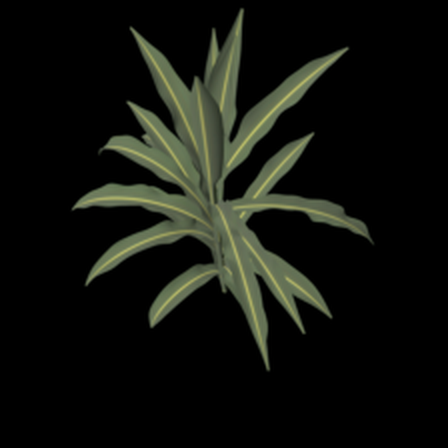
\includegraphics[width=0.4000in, height=0.4000in]{Figures/fig2/image.png}};
\node[anchor=south west, inner sep=0] at (0.9500,3.4600) {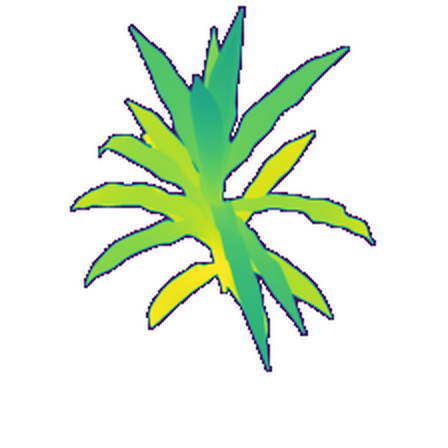
\includegraphics[width=0.4000in, height=0.4000in]{Figures/fig2/depth_image.png}};
\node[anchor=south west, inner sep=0] at (0.5200,3.0300) {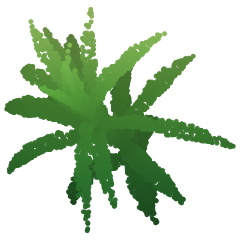
\includegraphics[width=0.4000in, height=0.4000in]{Figures/fig2/point_cloud.png}};
\node[anchor=south west, inner sep=0] at (0.9500,3.0300) {
\includegraphics[width=0.4000in, height=0.4000in]{Figures/fig2/parameters.png}};
\node[anchor=south west, inner sep=0] at (1.5500,3.4600) {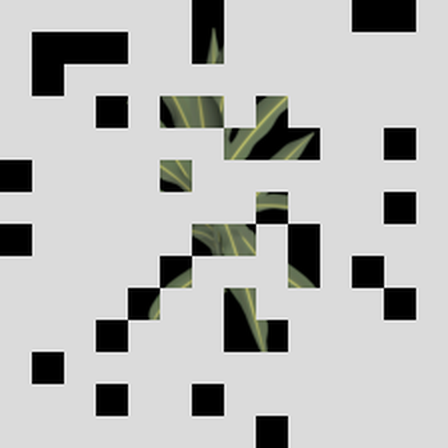
\includegraphics[width=0.4000in, height=0.4000in]{Figures/fig2/image_masked.png}};
\node[anchor=south west, inner sep=0] at (1.9800,3.4600) {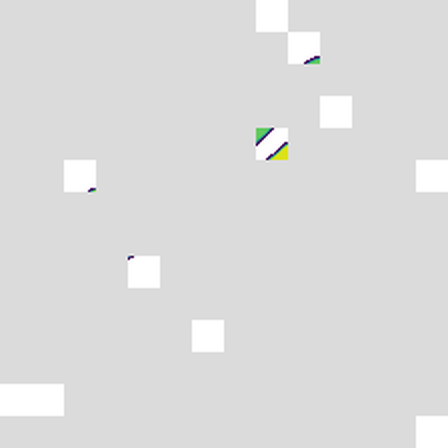
\includegraphics[width=0.4000in, height=0.4000in]{Figures/fig2/depth_masked.png}};
\node[anchor=south west, inner sep=0] at (1.5500,3.0300) {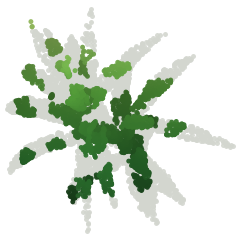
\includegraphics[width=0.4000in, height=0.4000in]{Figures/fig2/cloud_masked.png}};
\node[anchor=south west, inner sep=0] at (1.9800,3.0300) {
\includegraphics[width=0.4000in, height=0.4000in]{Figures/fig2/parameters_masked.png}};
\node[anchor=south west, inner sep=0] at (4.0600,3.4600) {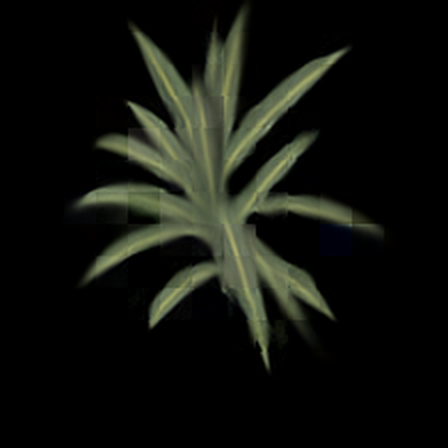
\includegraphics[width=0.4000in, height=0.4000in]{Figures/fig2/image_output.png}};
\node[anchor=south west, inner sep=0] at (4.4900,3.4600) {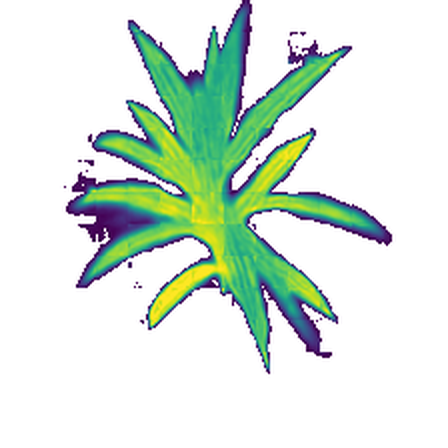
\includegraphics[width=0.4000in, height=0.4000in]{Figures/fig2/depth_output.png}};
\node[anchor=south west, inner sep=0] at (4.0600,3.0300) {
\includegraphics[width=0.4000in, height=0.4000in]{Figures/fig2/cloud_output.png}};
\node[anchor=south west, inner sep=0] at (4.4900,3.0300) {
\includegraphics[width=0.4000in, height=0.4000in]{Figures/fig2/parameters_output.png}};
\node[anchor=south west, inner sep=0] at (3.1950,3.7250) {
\includegraphics[width=0.1700in, height=0.1700in]{Figures/fig2/fire.png}};
\node[anchor=south west, inner sep=0] at (0.5950,2.0250) {
\includegraphics[width=0.1700in, height=0.1700in]{Figures/fig2/snow.png}};
\node[anchor=south west, inner sep=0] at (0.5800,1.6200) {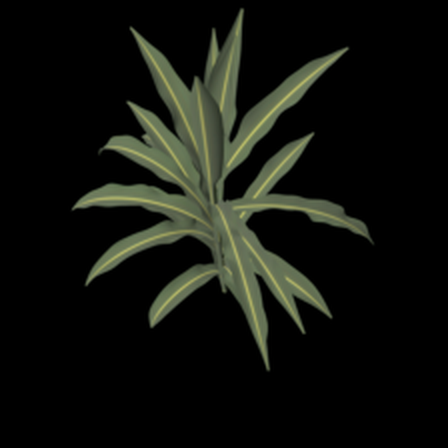
\includegraphics[width=0.2600in, height=0.2600in]{Figures/fig2/teacher_image.png}};
\node[anchor=south west, inner sep=0] at (0.8800,1.6200) {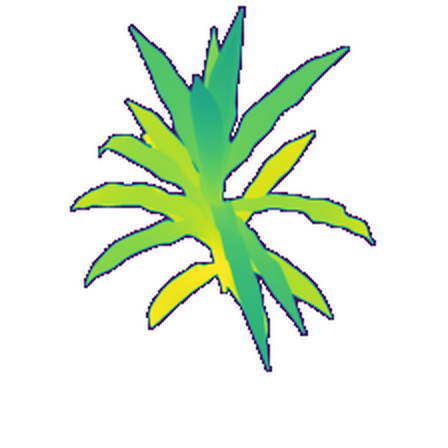
\includegraphics[width=0.2600in, height=0.2600in]{Figures/fig2/teacher_depth_image.png}};
\node[anchor=south west, inner sep=0] at (1.1800,1.6200) {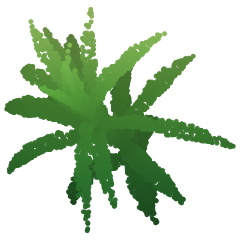
\includegraphics[width=0.2600in, height=0.2600in]{Figures/fig2/teacher_point_cloud.png}};
\node[anchor=south west, inner sep=0] at (1.4800,1.6200) {
\includegraphics[width=0.2600in, height=0.2600in]{Figures/fig2/teacher_parameters.png}};
\node[anchor=south west, inner sep=0] at (2.3750,2.0250) {
\includegraphics[width=0.1700in, height=0.1700in]{Figures/fig2/fire_2.png}};
\node[anchor=south west, inner sep=0] at (2.3600,1.6200) {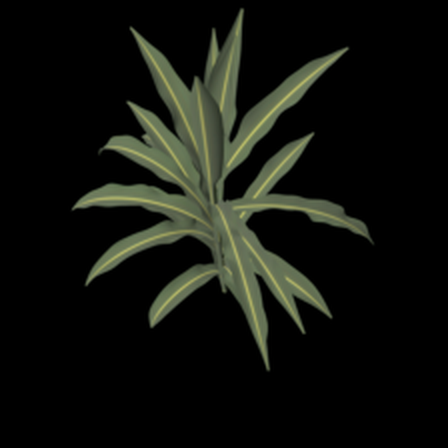
\includegraphics[width=0.2600in, height=0.2600in]{Figures/fig2/student_image.png}};
\node[anchor=south west, inner sep=0] at (2.6600,1.6200) {
\includegraphics[width=0.2600in, height=0.2600in]{Figures/fig2/student_hidden_0.png}};
\node[anchor=south west, inner sep=0] at (2.9600,1.6200) {
\includegraphics[width=0.2600in, height=0.2600in]{Figures/fig2/student_hidden_1.png}};
\node[anchor=south west, inner sep=0] at (3.2600,1.6200) {
\includegraphics[width=0.2600in, height=0.2600in]{Figures/fig2/student_hidden_2.png}};
\node[anchor=south west, inner sep=0] at (3.7500,1.6400) {
\includegraphics[width=0.5800in, height=0.5800in]{Figures/fig2/stage_2_before.png}};
\node[anchor=south west, inner sep=0] at (4.3700,1.6400) {
\includegraphics[width=0.5800in, height=0.5800in]{Figures/fig2/stage_2_after.png}};
\node[anchor=south west, inner sep=0] at (0.5200,0.4400) {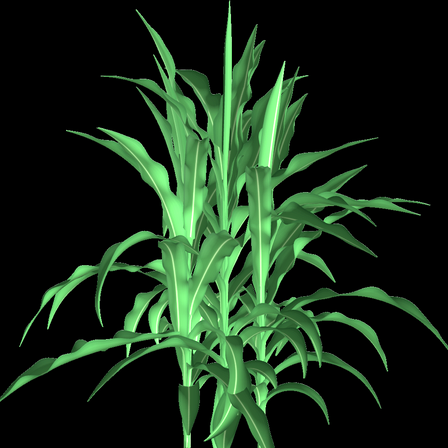
\includegraphics[width=0.4000in, height=0.4000in]{Figures/fig2/row_image.png}};
\node[anchor=south west, inner sep=0] at (0.9600,0.4400) {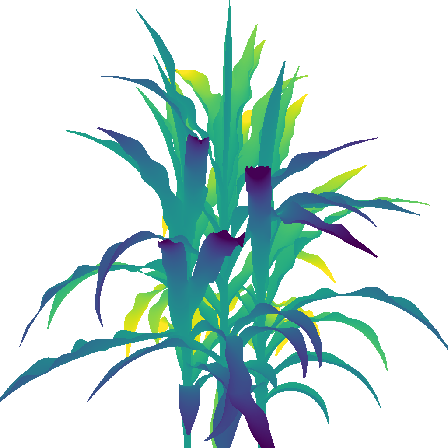
\includegraphics[width=0.4000in, height=0.4000in]{Figures/fig2/row_depth.png}};
\node[anchor=south west, inner sep=0] at (1.4000,0.4400) {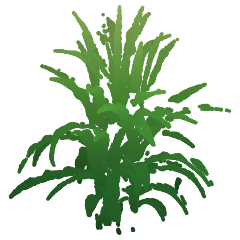
\includegraphics[width=0.4000in, height=0.4000in]{Figures/fig2/row_cloud.png}};
\node[anchor=south west, inner sep=0] at (2.7650,0.7250) {
\includegraphics[width=0.1700in, height=0.1700in]{Figures/fig2/fire_3.png}};
\node[anchor=south west, inner sep=0] at (3.7500,0.3800) {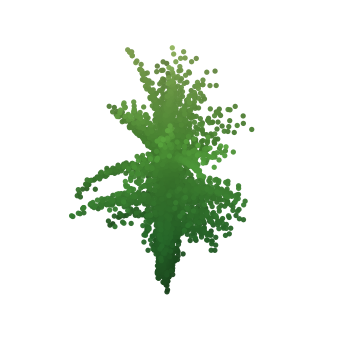
\includegraphics[width=0.5800in, height=0.5800in]{Figures/fig2/stage_3_before.png}};
\node[anchor=south west, inner sep=0] at (4.3700,0.3800) {
\includegraphics[width=0.5800in, height=0.5800in]{Figures/fig2/stage_3_after.png}};
\node[anchor=west, inner sep=0, outer sep=0, align=left, text=c1D221C, font={\fontsize{9.00}{11.25}\selectfont\sffamily\bfseries}] at (0.6300,4.2800) {Stage 1: masked pretraining};
\node[anchor=west, inner sep=0, outer sep=0, align=left, text=c1D221C, font={\fontsize{9.00}{11.25}\selectfont\sffamily\bfseries}] at (0.6300,2.5600) {Stage 2: cross-modal distillation};
\node[anchor=west, inner sep=0, outer sep=0, align=left, text=c1D221C, font={\fontsize{9.00}{11.25}\selectfont\sffamily\bfseries}] at (0.6300,1.2400) {Stage 3: row fine-tuning};
\draw[draw=cC0392B, line width=1.100pt, -{Triangle[length=2.80pt,width=2.80pt]}] (0.4000,3.4000) .. controls (0.1947,2.9333) and (0.1947,2.4667) .. (0.4000,2.0000);
\draw[draw=cC0392B, line width=1.100pt, -{Triangle[length=2.80pt,width=2.80pt]}] (0.4000,3.2000) .. controls (0.2137,2.3533) and (0.2137,1.5067) .. (0.4000,0.6600);
\node[anchor=center, inner sep=0, outer sep=0, align=center, text=cC0392B, font={\fontsize{9.00}{11.25}\selectfont\sffamily\bfseries}, rotate=90] at (0.1000,2.0000) {warm start};
\draw[draw=cC0392B, line width=0.800pt, rounded corners=0.0300in] (0.5200,3.4600) rectangle (0.9200,3.8600);
\draw[draw=cB8860B, line width=0.800pt, rounded corners=0.0300in] (0.9500,3.4600) rectangle (1.3500,3.8600);
\draw[draw=c2A9D8F, line width=0.800pt, rounded corners=0.0300in] (0.5200,3.0300) rectangle (0.9200,3.4300);
\draw[draw=c30638E, line width=0.800pt, rounded corners=0.0300in] (0.9500,3.0300) rectangle (1.3500,3.4300);
\draw[draw=cC0392B, line width=0.800pt, rounded corners=0.0300in] (1.5500,3.4600) rectangle (1.9500,3.8600);
\draw[draw=cB8860B, line width=0.800pt, rounded corners=0.0300in] (1.9800,3.4600) rectangle (2.3800,3.8600);
\draw[draw=c2A9D8F, line width=0.800pt, rounded corners=0.0300in] (1.5500,3.0300) rectangle (1.9500,3.4300);
\draw[draw=c30638E, line width=0.800pt, rounded corners=0.0300in] (1.9800,3.0300) rectangle (2.3800,3.4300);
\draw[draw=cC0392B, line width=0.800pt, rounded corners=0.0300in] (4.0600,3.4600) rectangle (4.4600,3.8600);
\draw[draw=cB8860B, line width=0.800pt, rounded corners=0.0300in] (4.4900,3.4600) rectangle (4.8900,3.8600);
\draw[draw=c2A9D8F, line width=0.800pt, rounded corners=0.0300in] (4.0600,3.0300) rectangle (4.4600,3.4300);
\draw[draw=c30638E, line width=0.800pt, rounded corners=0.0300in] (4.4900,3.0300) rectangle (4.8900,3.4300);
\node[anchor=south, inner sep=0, outer sep=0, align=center, text=c1D221C, font={\fontsize{9.00}{11.25}\selectfont\sffamily\bfseries}] at (0.9350,3.9600) {Input};
\node[anchor=south, inner sep=0, outer sep=0, align=center, text=c1D221C, font={\fontsize{9.00}{11.25}\selectfont\sffamily\bfseries}] at (1.9650,3.9600) {80 \% hidden};
\node[anchor=south, inner sep=0, outer sep=0, align=center, text=c1D221C, font={\fontsize{9.00}{11.25}\selectfont\sffamily\bfseries}] at (4.4750,3.9600) {Output};
\draw[draw=c1D221C, line width=0.900pt, -{Triangle[length=2.80pt,width=2.80pt]}] (1.3800,3.4450) -- (1.5200,3.4450);
\draw[draw=c1D221C, line width=0.900pt, -{Triangle[length=2.80pt,width=2.80pt]}] (2.4100,3.4450) -- (2.5900,3.4450);
\node[anchor=center, inner sep=0, outer sep=0, align=center, text=c2B3A67, font={\fontsize{9.00}{11.25}\selectfont\sffamily\bfseries}] at (2.9293,3.4450) {Encoder};
\node[anchor=center, inner sep=0, outer sep=0, align=center, text=c2B3A67, font={\fontsize{9.00}{11.25}\selectfont\sffamily\bfseries}] at (3.6137,3.4450) {Decoder};
\draw[draw=c1D221C, line width=0.900pt, -{Triangle[length=2.80pt,width=2.80pt]}] (3.9300,3.4450) -- (4.0300,3.4450);
\draw[draw=cC0392B, line width=0.900pt, -{Triangle[length=2.80pt,width=2.80pt]}, dash pattern=on 2.70pt off 1.80pt] (4.4750,2.9500) -- (0.9350,2.9500);
\node[anchor=north, inner sep=0, outer sep=0, align=center, text=cC0392B, font={\fontsize{9.00}{11.25}\selectfont\sffamily}] at (2.6900,2.9000) {loss on the hidden tokens};
\node[anchor=west, inner sep=0, outer sep=0, align=left, text=c1D221C, font={\fontsize{9.00}{11.25}\selectfont\sffamily\bfseries}] at (0.8000,2.1100) {Teacher};
\draw[draw=cC0392B, line width=0.600pt, rounded corners=0.0300in] (0.5800,1.6200) rectangle (0.8400,1.8800);
\draw[draw=cB8860B, line width=0.600pt, rounded corners=0.0300in] (0.8800,1.6200) rectangle (1.1400,1.8800);
\draw[draw=c2A9D8F, line width=0.600pt, rounded corners=0.0300in] (1.1800,1.6200) rectangle (1.4400,1.8800);
\draw[draw=c30638E, line width=0.600pt, rounded corners=0.0300in] (1.4800,1.6200) rectangle (1.7400,1.8800);
\draw[draw=cC0392B, line width=0.900pt, -{Triangle[length=2.80pt,width=2.80pt]}, dash pattern=on 2.70pt off 1.80pt] (1.8000,1.8800) -- (2.2700,1.8800);
\node[anchor=south, inner sep=0, outer sep=0, align=center, text=cC0392B, font={\fontsize{9.00}{11.25}\selectfont\sffamily}] at (2.0350,1.9300) {features};
\node[anchor=west, inner sep=0, outer sep=0, align=left, text=c2B3A67, font={\fontsize{9.00}{11.25}\selectfont\sffamily\bfseries}] at (2.5800,2.1100) {Student};
\draw[draw=cC0392B, line width=0.900pt, rounded corners=0.0300in] (2.3600,1.6200) rectangle (2.6200,1.8800);
\draw[draw=cB8860B, line width=0.600pt, dash pattern=on 1.80pt off 1.20pt, rounded corners=0.0300in] (2.6600,1.6200) rectangle (2.9200,1.8800);
\draw[draw=c2A9D8F, line width=0.600pt, dash pattern=on 1.80pt off 1.20pt, rounded corners=0.0300in] (2.9600,1.6200) rectangle (3.2200,1.8800);
\draw[draw=c30638E, line width=0.600pt, dash pattern=on 1.80pt off 1.20pt, rounded corners=0.0300in] (3.2600,1.6200) rectangle (3.5200,1.8800);
\draw[draw=c1D221C, line width=0.900pt, -{Triangle[length=2.80pt,width=2.80pt]}] (3.5800,1.9100) -- (3.7200,1.9100);
\draw[draw=c5F685C, line width=0.800pt, dash pattern=on 2.40pt off 1.60pt, rounded corners=0.0300in] (3.7500,1.6400) rectangle (4.3300,2.2200);
\node[anchor=south, inner sep=0, outer sep=0, align=center, text=c5F685C, font={\fontsize{9.00}{11.25}\selectfont\sffamily}] at (4.0400,2.2700) {before};
\draw[draw=c2A9D8F, line width=0.800pt, rounded corners=0.0300in] (4.3700,1.6400) rectangle (4.9500,2.2200);
\node[anchor=south, inner sep=0, outer sep=0, align=center, text=c2B3A67, font={\fontsize{9.00}{11.25}\selectfont\sffamily\bfseries}] at (4.6600,2.2700) {after};
\node[anchor=north, inner sep=0, outer sep=0, align=center, text=c1D221C, font={\fontsize{9.00}{11.25}\selectfont\sffamily}] at (4.3500,1.5800) {Chamfer 2.27 $\rightarrow$ 0.88};
\draw[draw=cC0392B, line width=0.800pt, rounded corners=0.0300in] (0.5200,0.4400) rectangle (0.9200,0.8400);
\draw[draw=cB8860B, line width=0.800pt, rounded corners=0.0300in] (0.9600,0.4400) rectangle (1.3600,0.8400);
\draw[draw=c2A9D8F, line width=0.800pt, rounded corners=0.0300in] (1.4000,0.4400) rectangle (1.8000,0.8400);
\node[anchor=south, inner sep=0, outer sep=0, align=center, text=c1D221C, font={\fontsize{9.00}{11.25}\selectfont\sffamily\bfseries}] at (1.1600,0.9200) {Crop row};
\draw[draw=c1D221C, line width=0.900pt, -{Triangle[length=2.80pt,width=2.80pt]}] (1.8500,0.6400) -- (2.2000,0.6400);
\node[anchor=center, inner sep=0, outer sep=0, align=center, text=c2B3A67, font={\fontsize{9.00}{11.25}\selectfont\sffamily\bfseries}] at (2.5194,0.6400) {Enc};
\node[anchor=center, inner sep=0, outer sep=0, align=center, text=c2B3A67, font={\fontsize{9.00}{11.25}\selectfont\sffamily\bfseries}] at (3.1621,0.6400) {Dec};
\node[anchor=north, inner sep=0, outer sep=0, align=center, text=cC0392B, font={\fontsize{9.00}{11.25}\selectfont\sffamily}] at (2.8300,0.3500) {loss: center plant only};
\draw[draw=c1D221C, line width=0.900pt, -{Triangle[length=2.80pt,width=2.80pt]}] (3.4600,0.6400) -- (3.7200,0.6400);
\draw[draw=c5F685C, line width=0.800pt, dash pattern=on 2.40pt off 1.60pt, rounded corners=0.0300in] (3.7500,0.3800) rectangle (4.3300,0.9600);
\node[anchor=south, inner sep=0, outer sep=0, align=center, text=c5F685C, font={\fontsize{9.00}{11.25}\selectfont\sffamily}] at (4.0400,1.0100) {before};
\draw[draw=c2A9D8F, line width=0.800pt, rounded corners=0.0300in] (4.3700,0.3800) rectangle (4.9500,0.9600);
\node[anchor=south, inner sep=0, outer sep=0, align=center, text=c2B3A67, font={\fontsize{9.00}{11.25}\selectfont\sffamily\bfseries}] at (4.6600,1.0100) {after};
\node[anchor=north, inner sep=0, outer sep=0, align=center, text=c1D221C, font={\fontsize{9.00}{11.25}\selectfont\sffamily}] at (4.3500,0.3200) {Chamfer 230 $\rightarrow$ 31};
\node[anchor=center, inner sep=0, outer sep=0, align=center, text=c1D221C, font={\fontsize{9.00}{11.25}\selectfont\sffamily\bfseries}] at (5.9775,4.0600) {Inside CropCode};
\node[anchor=west, inner sep=0, outer sep=0, align=left, text=cC0392B, font={\fontsize{9.00}{11.25}\selectfont\sffamily\bfseries}] at (5.9250,3.7100) {Image  196};
\node[anchor=west, inner sep=0, outer sep=0, align=left, text=cB8860B, font={\fontsize{9.00}{11.25}\selectfont\sffamily\bfseries}] at (5.9250,3.4100) {Depth  196};
\node[anchor=west, inner sep=0, outer sep=0, align=left, text=c2A9D8F, font={\fontsize{9.00}{11.25}\selectfont\sffamily\bfseries}] at (5.9250,3.1100) {Cloud  196};
\node[anchor=west, inner sep=0, outer sep=0, align=left, text=c30638E, font={\fontsize{9.00}{11.25}\selectfont\sffamily\bfseries}] at (5.9250,2.8100) {Params  1+K};
\node[anchor=west, inner sep=0, outer sep=0, align=left, text=c5F685C, font={\fontsize{9.00}{11.25}\selectfont\sffamily}] at (5.2400,2.5200) {tokens (hollow = hidden)};
\node[anchor=west, inner sep=0, outer sep=0, align=left, text=c1D221C, font={\fontsize{9.00}{11.25}\selectfont\sffamily\bfseries}] at (5.2400,2.2000) {Dirichlet split};
\node[anchor=west, inner sep=0, outer sep=0, align=left, text=c5F685C, font={\fontsize{9.00}{11.25}\selectfont\sffamily}] at (5.2400,1.7600) {of the visible tokens};
\node[anchor=center, inner sep=0, outer sep=0, align=center, text=c2B3A67, font={\fontsize{9.00}{11.25}\selectfont\sffamily\bfseries}] at (5.9775,1.2700) {Encoder, 12 blocks};
\node[anchor=center, inner sep=0, outer sep=0, align=center, text=c2B3A67, font={\fontsize{9.00}{11.25}\selectfont\sffamily\bfseries}] at (5.9775,0.7100) {Decoder, 8 blocks};
\draw[draw=c2B3A67, line width=0.800pt, -{Triangle[length=2.80pt,width=2.80pt]}] (5.9775,1.6200) -- (5.9775,1.4900);
\draw[draw=c2B3A67, line width=0.800pt, -{Triangle[length=2.80pt,width=2.80pt]}] (5.9775,1.0500) -- (5.9775,0.9300);
\draw[draw=c2B3A67, line width=0.800pt, -{Triangle[length=2.80pt,width=2.80pt]}] (5.9775,0.4900) -- (5.9775,0.4200);
\node[anchor=center, inner sep=0, outer sep=0, align=center, text=c2B3A67, font={\fontsize{9.00}{11.25}\selectfont\sffamily}] at (5.9775,0.3200) {one head per stream};
\end{tikzpicture}%
}%
}
  \caption{\textbf{\method{} in three training stages.} Stage~1: the four streams of a plant are tokenized, 80\% of the tokens are hidden under a Dirichlet split across streams, and a shared encoder and decoder reconstruct every stream (image, depth and parameter losses on the hidden tokens; the point-cloud loss, QAL plus Sinkhorn, on the whole cloud). The procedural parameters are drawn as a stem-and-leaves schematic. Stage~2: a frozen teacher that reads all four streams passes its decoder features and latent to a student that reads one stream; shown is the point cloud generated from the image alone before and after distillation. Stage~3: fine-tuning on crop rows with the loss taken against the center plant alone; shown is the center plant written from the row before (no row fine-tuning) and after. Chamfer: sorghum test means from Table~\ref{tab:anysubset} ($\times10^{-3}$) and Table~\ref{tab:rows} (all streams, $\times10^{-4}\,\mathrm{m}^2$), both in Appendix~\ref{app:tables}. Stages~2 and~3 start from the Stage~1 weights. Examples: one held-out sorghum test plant and row.}
  \label{fig:arch}
\end{figure*}

\method{} makes this inverse problem tractable by using the
procedural generator itself as the prior. We pretrain a four-stream masked
autoencoder~\citep{he2022mae,bachmann2022multimae,mizrahi2023fourm,
dong2025embodiedmae} over RGB, depth, point clouds and tokenized procedural
parameters of 15{,}000 generated plants per species (maize and sorghum),
fine-tune it on simulated rows whose neighboring leaves bend on contact,
and distill a full-modality teacher~\citep{hinton2015distillation} into
single-sensor students; random modality subsets are masked in pretraining,
so one model completes any subset at inference. Distillation lowers the
cross-modal generation loss by 30\% in sorghum and 44\% in maize and halves
the sorghum parameter error from a point cloud alone; row fine-tuning
removes 92\% (maize) and 85\% (sorghum) of the error the neighbors add. We
also answer a design question that arises for any model with access to
generative structure: a parameter stream largely visible to the encoder
harms the representation in both species, while budget-matched controls
show its value as a pure reconstruction target depends on the generator
(it degrades sorghum and improves maize). Supervising parameters as a
generation target still lets the distilled generalist beat a
parameter-only specialist at parameter regression (recipe MAE from the
point cloud 0.019 against 0.036), consistent with modality
competition~\citep{peng2022ogm} and negative transfer~\citep{yu2020pcgrad}
from a stream that already contains the answer. Finally, depth lowers
Chamfer by 25--28\% while a frozen-representation probe finds little gain
from it and identifies RGB as the main source of trait information: on
slender geometry the two metrics measure different quantities, and we adopt
the probe as the deciding metric~\citep{chen2020simclr,wu2021dcd}.

We claim that fragmentary field sensing suffices to recover a complete,
interpretable procedural plant, provided the generator is used for both the
training data and the output representation.
We test this claim on rows built from real maize and sorghum plants
with independently reconstructed ground
truth~\citep{maizefield3d2025,hadadi2026vlmmaize}, in which neighbors occlude
the target: zero-shot, accuracy degrades on plants outside the generator's
size range, and fine-tuning on 75\% of the real plants recovers the held-out
plants' height to a 1.6\% median error and their leaf count to within one
leaf on 70\% of maize stops, in milliseconds per plant.
The key contributions of this work are:
\begin{enumerate}
  \item \textbf{Task and framework.} The first formulation and system,
  to our knowledge, for recovering procedural plant representations of
  slender, row-occluded field crops from \emph{any subset} of RGB, depth,
  and point-cloud input in one amortized forward pass, with full-modal to
  single-sensor distillation (generation loss $-30\%$ in sorghum and
  $-44\%$ in maize; sorghum parameter error from a point cloud alone
  halved), and row fine-tuning that removes most of the error added by
  neighboring plants (92\% in maize, 85\% in sorghum).
  \item \textbf{A design rule for structured modalities.} Controlled,
  budget-matched, two-species evidence that a parameter stream largely
  visible to the encoder degrades the sensor representation in both
  species, while the value of the parameters as a reconstruction target
  depends on the generator (it degrades the sorghum representation and
  improves the maize one); we expect this guidance to transfer to any
  multimodal model with access to privileged generative structure.
  \item \textbf{An evaluation protocol for slender geometry.} A
  demonstration that Chamfer distance and downstream phenotype probes
  disagree systematically on slender organs, and a frozen-latent probe
  protocol that resolves modality decisions where Chamfer is insensitive.
  \item \textbf{A benchmark.} \dataset{}, a two-species procedural
  field benchmark of 30{,}000 plants spanning diverse phenotypes, generator
  configurations, and row occlusion severities, with paired multimodal
  captures, physically simulated row occlusion, and exact parameter ground
  truth, together with a real-field evaluation split carrying reconstructed
  procedural ground truth across the genotypes of a diversity
  panel~\citep{maizefield3d2025}. No existing dataset combines these
  elements (Tab.~\ref{tab:datacompare})~\citep{schunck2021pheno4d,yuan2018pcn}.
  We will release the data, generation code, and evaluation scripts.
\end{enumerate}
%%%%%%%%%%%%%%%%%%%%%%%%%%%%%%%%%%%%%%%%%%%%%%%%%%%%%%%%%%%%%%%%%%%%%%%%%%%
% ==== end sec/1_intro.tex ====
%%%%%%%%%%%%%%%%%%%%%%%%%%%%%%%%%%%%%%%%%%%%%%%%%%%%%%%%%%%%%%%%%%%%%%%%%%%
%%%%%%%%%%%%%%%%%%%%%%%%%%%%%%%%%%%%%%%%%%%%%%%%%%%%%%%%%%%%%%%%%%%%%%%%%%%
% ==== sec/2_related.tex (inlined) ====
%%%%%%%%%%%%%%%%%%%%%%%%%%%%%%%%%%%%%%%%%%%%%%%%%%%%%%%%%%%%%%%%%%%%%%%%%%%
\section{Related Work}
\label{sec:related}

Appendix~\ref{app:litreview} reviews each of these literatures in
detail; here we state what distinguishes our setting.

\noindent\textbf{Recovering procedural plants.}
Tree-generator parameters have been recovered per instance by
stochastic search~\citep{stava2014ipmtrees}, MCMC
inference~\citep{talton2011metropolis} and L-system
induction~\citep{guo2020ipmlsys,latentlsys2023}; recent crop systems learn
parametric morphology from clean point
clouds~\citep{demeter2025,ghrer2025paramplants}, fit procedural models
against multi-view imagery~\citep{cropcraft2026}, or reconstruct procedural
maize from terrestrial laser scans through a staged vision-language
pipeline~\citep{hadadi2026vlmmaize,nurbsdiff2022}. Each presupposes a single
rich observation of an isolated plant; none addresses missing modalities or
inter-plant occlusion.

\noindent\textbf{Programs from observations.}
Shape programs~\citep{shapeprograms2019}, diffusion-based inverse
procedural content generation~\citep{zhao2025dipcg} and CAD
generation~\citep{text2cad2024,kolodiazhnyi2025cadrille} decode parametric
programs from observations, but for rigid objects observed cleanly and in
isolation, and none asks whether the program parameters should be visible to
the encoder at all.

\noindent\textbf{Completion and slender geometry.}
Learned point cloud
completion~\citep{yuan2018pcn,yu2021pointr,yu2023adapointr,cai2024einet}
trains on compact, largely convex benchmarks; completion of occluded plant
organs~\citep{lee2026occ} and thin-structure
reconstruction~\citep{curvegaussian2025,qi2026rethinking} output
unstructured geometry rather than an editable model. Chamfer distance is
structurally insensitive to thin
sheets~\citep{wu2021dcd,song2026structural,lin2023infocd}, so we evaluate
with trait probes alongside geometric metrics (Sec.~\ref{sec:exp-metrics}).

\noindent\textbf{Multimodal masked pretraining and synthetic data.}
Masked autoencoding~\citep{he2022mae} extends to multiple
modalities~\citep{bachmann2022multimae}, any-to-any
generation~\citep{mizrahi2023fourm,bachmann2024fourm21}, point
clouds~\citep{pang2022pointmae} and combined RGB, depth and point cloud
inputs in EmbodiedMAE, on which our architecture is
based~\citep{dong2025embodiedmae}. We add a structured generative modality
encoded with continuous number tokens~\citep{golkar2023xval} and distill a
generative full-modality teacher~\citep{hinton2015distillation} into
single-sensor students, with missing-modality robustness a recognized
concern~\citep{wang2024robustmissing}. Pretraining on purely synthetic data
is viable from fractals to procedural
scenes~\citep{kataoka2020fractaldb,raistrick2023infinigen,greff2022kubric},
with domain randomization reducing the gap~\citep{tobin2017domainrand} and
task alignment setting its value~\citep{fan2023intriguing}; our setting is
the favorable case, since the generator defines the output representation
and is paired with real field evaluation data~\citep{maizefield3d2025}, and
our caveat is that exposing most of its parameters to the encoder reduces
representation quality in both species (Sec.~\ref{sec:exp-params}).

\section{Method}
\label{sec:method}

We formulate the inverse problem (Sec.~\ref{sec:method-form}), build
the \dataset{} data engine (Sec.~\ref{sec:method-data}), pretrain a
four-stream masked autoencoder (Sec.~\ref{sec:method-pretrain}), distill it
into single-sensor students (Sec.~\ref{sec:method-distill}) and define the
evaluation protocols; Fig.~\ref{fig:arch} gives the
overview.


\subsection{Problem formulation: inverse procedural reconstruction}
\label{sec:method-form}

A procedural generator $G$ maps a parameter vector
$\theta \in \R^{d_\theta}$ to an editable 3D mesh $G(\theta)$; $\theta$
describes the plant completely, from stem height and internode spacing to
each leaf's insertion height, blade length and width, and insertion, roll
and azimuth angles. Field sensors yield partial, noisy, occluded
observations: from the modality universe
$\mathcal{M} = \{\mathrm{rgb}, \mathrm{d}, \mathrm{pc}\}$ a campaign
acquires some subset $S \subseteq \mathcal{M}$, and row neighbors occlude
the target. We learn an amortized feed-forward inverse
\begin{equation}
  f_\phi\!\left(\{x^m : m \in S\}\right)
  = \left(\hat\theta, \{\hat x^m : m \in \mathcal{M}\}\right),
  \label{eq:procedural-inverse}
\end{equation}
returning the predicted recipe $\hat\theta$ and the completed
streams. Where raw geometric completion can only guess hidden points,
predicting $\hat\theta$ uses $G$ as the prior: $G(\hat\theta)$ is
structurally complete, editable and interpretable in agronomic traits, and
the inversion runs in one forward pass of milliseconds instead of minutes
to hours of per-plant optimization.

\subsection{A procedural field-data engine: \dataset{}}
\label{sec:method-data}

To train and evaluate \method{}, we construct \dataset{}, a synthetic
benchmark pairing exact procedural ground-truth parameters with multimodal
field observations under realistic row neighbor occlusion
(Tab.~\ref{tab:fieldproc}). Figure~\ref{fig:dataset} shows, for each
species, sample plants, the four streams of one view, cameras of one plant and a row
scene.

\begin{figure*}[t]
  \centering
  \resizebox{\linewidth}{!}{% Fig. 3 (the dataset) as native TikZ, written by figures/make_dataset_fig_v2.py (do not edit by hand: re-run it).
% Tiles in Figures/fig3/; boxes, leader lines and text are TikZ, text in \sffamily (Helvetica under cvpr/times).
% Natural size 6.875 x 3.86 in; include with \resizebox{\textwidth}{!}{% Fig. 3 (the dataset) as native TikZ, written by figures/make_dataset_fig_v2.py (do not edit by hand: re-run it).
% Tiles in Figures/fig3/; boxes, leader lines and text are TikZ, text in \sffamily (Helvetica under cvpr/times).
% Natural size 6.875 x 3.86 in; include with \resizebox{\textwidth}{!}{% Fig. 3 (the dataset) as native TikZ, written by figures/make_dataset_fig_v2.py (do not edit by hand: re-run it).
% Tiles in Figures/fig3/; boxes, leader lines and text are TikZ, text in \sffamily (Helvetica under cvpr/times).
% Natural size 6.875 x 3.86 in; include with \resizebox{\textwidth}{!}{\input{Figures/fig_dataset_tikz}}.
\definecolor{c111111}{HTML}{111111}%
\definecolor{c333333}{HTML}{333333}%
\definecolor{c3F5F8F}{HTML}{3F5F8F}%
\definecolor{c444444}{HTML}{444444}%
\definecolor{c555555}{HTML}{555555}%
\definecolor{c5E4A96}{HTML}{5E4A96}%
\definecolor{c809EC2}{HTML}{809EC2}%
\definecolor{c9A9A9A}{HTML}{9A9A9A}%
\definecolor{c9D8CC4}{HTML}{9D8CC4}%
\definecolor{cA07800}{HTML}{A07800}%
\definecolor{cA8456E}{HTML}{A8456E}%
\definecolor{cD091A7}{HTML}{D091A7}%
\definecolor{cE0B020}{HTML}{E0B020}%
\definecolor{cE6ECF3}{HTML}{E6ECF3}%
\definecolor{cEAE7F2}{HTML}{EAE7F2}%
\definecolor{cF4F4F5}{HTML}{F4F4F5}%
\definecolor{cF6E9ED}{HTML}{F6E9ED}%
\definecolor{cFAF2D4}{HTML}{FAF2D4}%
\begin{tikzpicture}[x=1in, y=1in]
\useasboundingbox (0,0) rectangle (6.875,3.86);
\node[anchor=base west, inner sep=0, text=c111111, rotate=0, font={\fontsize{9.0}{10.8}\selectfont\sffamily\bfseries}] at (0.0200,3.7200) {a};
\node[anchor=base west, inner sep=0, text=c111111, rotate=0, font={\fontsize{6.2}{7.4}\selectfont\sffamily}] at (0.1800,3.7200) {The plants: 15,000 per species (6 shown)};
\node[anchor=base west, inner sep=0, text=c111111, rotate=0, font={\fontsize{9.0}{10.8}\selectfont\sffamily\bfseries}] at (2.3800,3.7200) {b};
\node[anchor=base west, inner sep=0, text=c111111, rotate=0, font={\fontsize{6.2}{7.4}\selectfont\sffamily}] at (2.5400,3.7200) {One view of the boxed plant as its four streams};
\draw[draw=c809EC2, line width=1.00pt, rounded corners=4.32pt, fill=cE6ECF3] (0.2400,2.4100) rectangle (1.7500,3.4450);
\node[anchor=center, inner sep=0, text=c111111, rotate=90, font={\fontsize{7.0}{8.4}\selectfont\sffamily\bfseries}] at (0.1500,2.9275) {sorghum};
\node[anchor=south west, inner sep=0] at (0.3000,2.9450) {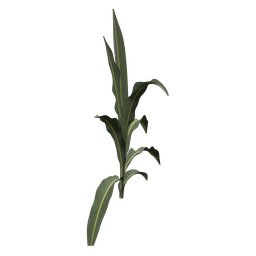
\includegraphics[width=0.4400in, height=0.4400in]{Figures/fig3/sorghum_gallery_0.png}};
\node[anchor=south west, inner sep=0] at (0.7750,2.9450) {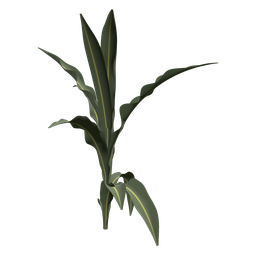
\includegraphics[width=0.4400in, height=0.4400in]{Figures/fig3/sorghum_gallery_1.png}};
\node[anchor=south west, inner sep=0] at (1.2500,2.9450) {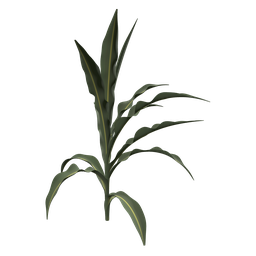
\includegraphics[width=0.4400in, height=0.4400in]{Figures/fig3/sorghum_gallery_2.png}};
\node[anchor=south west, inner sep=0] at (0.3000,2.4700) {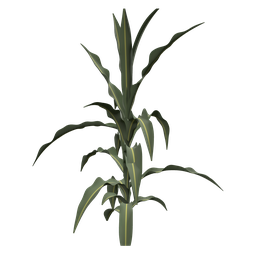
\includegraphics[width=0.4400in, height=0.4400in]{Figures/fig3/sorghum_gallery_3.png}};
\node[anchor=south west, inner sep=0] at (0.7750,2.4700) {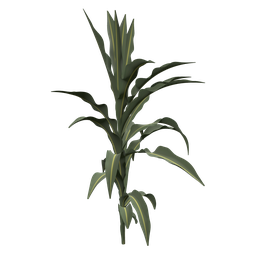
\includegraphics[width=0.4400in, height=0.4400in]{Figures/fig3/sorghum_gallery_4.png}};
\node[anchor=south west, inner sep=0] at (1.2500,2.4700) {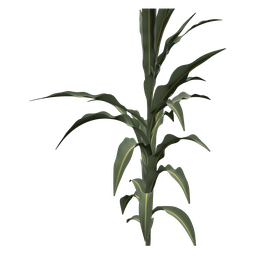
\includegraphics[width=0.4400in, height=0.4400in]{Figures/fig3/sorghum_gallery_5.png}};
\draw[draw=c333333, line width=1.00pt, rounded corners=2.16pt] (1.2350,2.4550) rectangle (1.7050,2.9250);
\draw[draw=c9A9A9A, line width=0.60pt] (1.7050,2.9250) -- (2.3700,3.4175);
\draw[draw=c9A9A9A, line width=0.60pt] (1.7050,2.4550) -- (2.3700,2.4375);
\draw[draw=c9A9A9A, line width=1.00pt, rounded corners=4.32pt, fill=cF4F4F5] (2.3700,2.4375) rectangle (6.8050,3.4175);
\draw[draw=c809EC2, line width=1.00pt, rounded corners=3.60pt, fill=cE6ECF3] (2.4100,2.4775) rectangle (3.3100,3.3775);
\node[anchor=south west, inner sep=0] at (2.4400,2.5075) {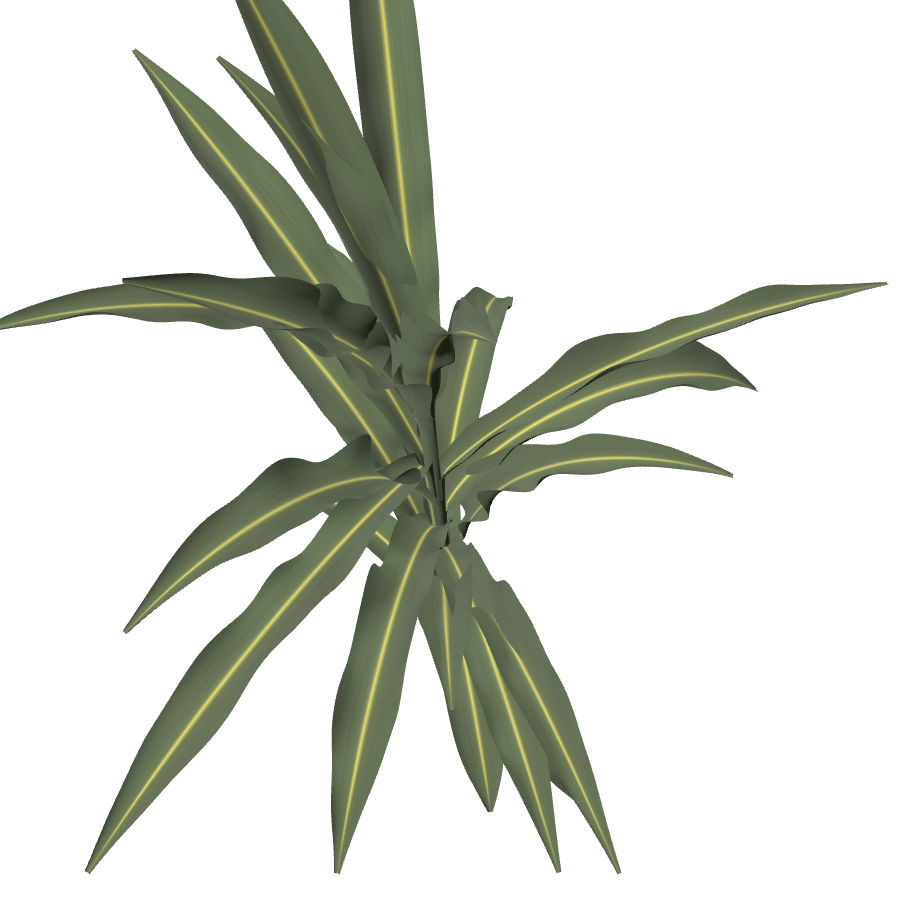
\includegraphics[width=0.8400in, height=0.8400in]{Figures/fig3/sorghum_rgb.png}};
\node[anchor=base, inner sep=0, text=c3F5F8F, rotate=0, font={\fontsize{6.2}{7.4}\selectfont\sffamily\bfseries}] at (2.8600,3.4925) {Image};
\draw[draw=cE0B020, line width=1.00pt, rounded corners=3.60pt, fill=cFAF2D4] (3.5617,2.4775) rectangle (4.4617,3.3775);
\node[anchor=south west, inner sep=0] at (3.5917,2.5075) {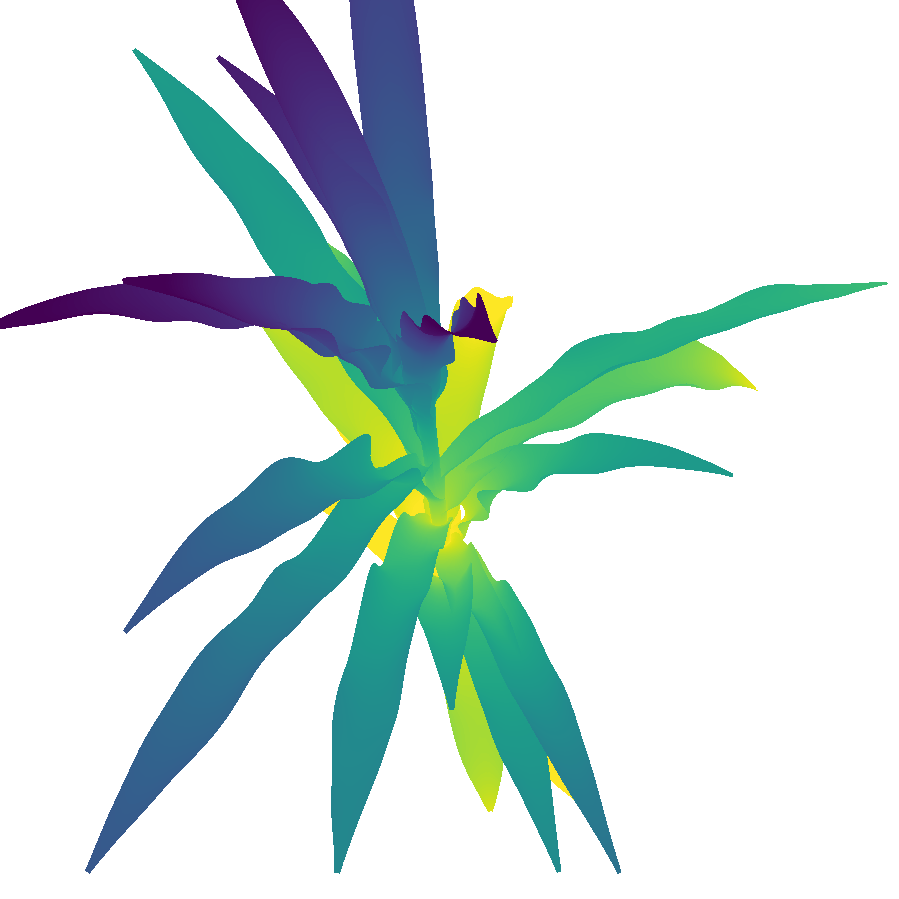
\includegraphics[width=0.8400in, height=0.8400in]{Figures/fig3/sorghum_depth.png}};
\node[anchor=base, inner sep=0, text=cA07800, rotate=0, font={\fontsize{6.2}{7.4}\selectfont\sffamily\bfseries}] at (4.0117,3.4925) {Depth image};
\draw[draw=cD091A7, line width=1.00pt, rounded corners=3.60pt, fill=cF6E9ED] (4.7133,2.4775) rectangle (5.6133,3.3775);
\node[anchor=south west, inner sep=0] at (4.7433,2.5075) {
\includegraphics[width=0.8400in, height=0.8400in]{Figures/fig3/sorghum_pc.png}};
\node[anchor=base, inner sep=0, text=cA8456E, rotate=0, font={\fontsize{6.2}{7.4}\selectfont\sffamily\bfseries}] at (5.1633,3.4925) {Point cloud};
\draw[draw=c9D8CC4, line width=1.00pt, rounded corners=3.60pt, fill=cEAE7F2] (5.8650,2.4775) rectangle (6.7650,3.3775);
\node[anchor=south west, inner sep=0] at (5.8950,2.5075) {
\includegraphics[width=0.8400in, height=0.8400in]{Figures/fig3/sorghum_text.png}};
\node[anchor=base, inner sep=0, text=c5E4A96, rotate=0, font={\fontsize{6.2}{7.4}\selectfont\sffamily\bfseries}] at (6.3150,3.4925) {Procedural parameters};
\draw[draw=c809EC2, line width=1.00pt, rounded corners=4.32pt, fill=cE6ECF3] (0.2400,1.3100) rectangle (1.7500,2.3450);
\node[anchor=center, inner sep=0, text=c111111, rotate=90, font={\fontsize{7.0}{8.4}\selectfont\sffamily\bfseries}] at (0.1500,1.8275) {maize};
\node[anchor=south west, inner sep=0] at (0.3000,1.8450) {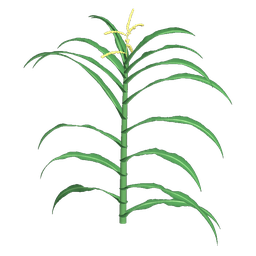
\includegraphics[width=0.4400in, height=0.4400in]{Figures/fig3/maize_gallery_0.png}};
\node[anchor=south west, inner sep=0] at (0.7750,1.8450) {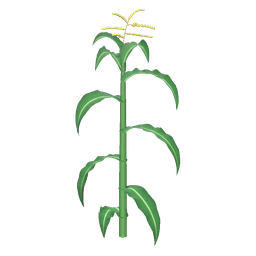
\includegraphics[width=0.4400in, height=0.4400in]{Figures/fig3/maize_gallery_1.png}};
\node[anchor=south west, inner sep=0] at (1.2500,1.8450) {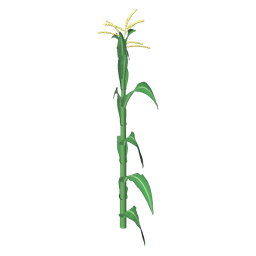
\includegraphics[width=0.4400in, height=0.4400in]{Figures/fig3/maize_gallery_2.png}};
\node[anchor=south west, inner sep=0] at (0.3000,1.3700) {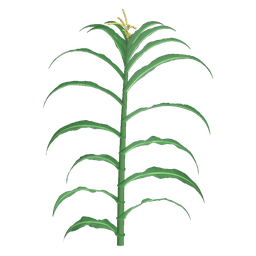
\includegraphics[width=0.4400in, height=0.4400in]{Figures/fig3/maize_gallery_3.png}};
\node[anchor=south west, inner sep=0] at (0.7750,1.3700) {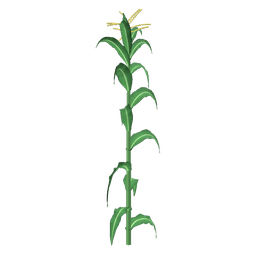
\includegraphics[width=0.4400in, height=0.4400in]{Figures/fig3/maize_gallery_4.png}};
\node[anchor=south west, inner sep=0] at (1.2500,1.3700) {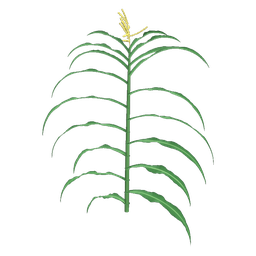
\includegraphics[width=0.4400in, height=0.4400in]{Figures/fig3/maize_gallery_5.png}};
\draw[draw=c333333, line width=1.00pt, rounded corners=2.16pt] (1.2350,1.3550) rectangle (1.7050,1.8250);
\draw[draw=c9A9A9A, line width=0.60pt] (1.7050,1.8250) -- (2.3700,2.3175);
\draw[draw=c9A9A9A, line width=0.60pt] (1.7050,1.3550) -- (2.3700,1.3375);
\draw[draw=c9A9A9A, line width=1.00pt, rounded corners=4.32pt, fill=cF4F4F5] (2.3700,1.3375) rectangle (6.8050,2.3175);
\draw[draw=c809EC2, line width=1.00pt, rounded corners=3.60pt, fill=cE6ECF3] (2.4100,1.3775) rectangle (3.3100,2.2775);
\node[anchor=south west, inner sep=0] at (2.4400,1.4075) {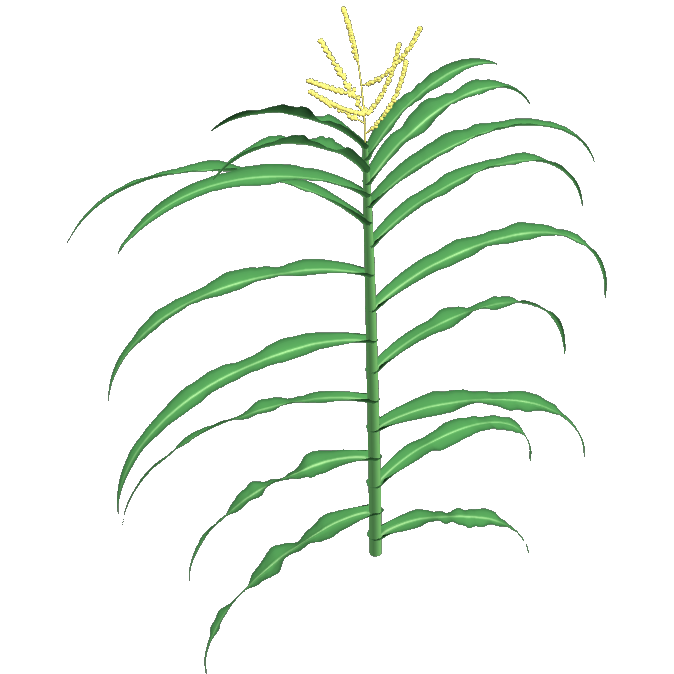
\includegraphics[width=0.8400in, height=0.8400in]{Figures/fig3/maize_rgb.png}};
\draw[draw=cE0B020, line width=1.00pt, rounded corners=3.60pt, fill=cFAF2D4] (3.5617,1.3775) rectangle (4.4617,2.2775);
\node[anchor=south west, inner sep=0] at (3.5917,1.4075) {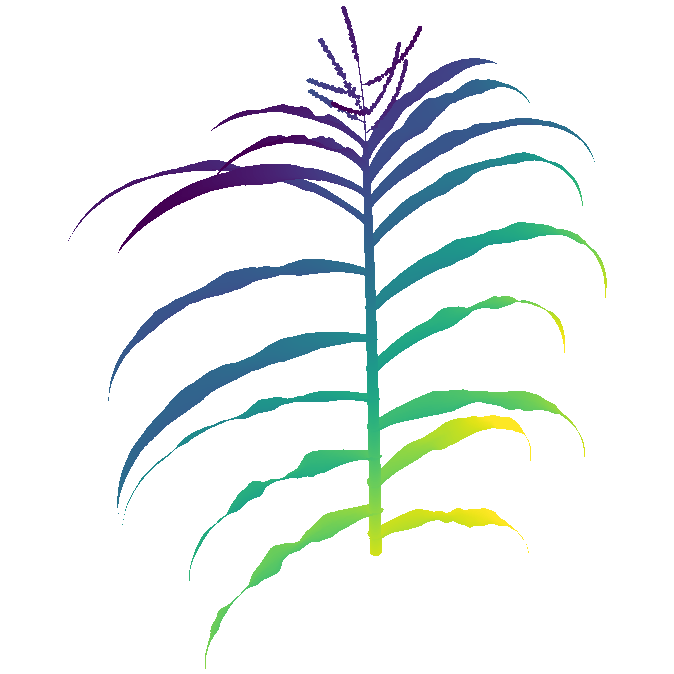
\includegraphics[width=0.8400in, height=0.8400in]{Figures/fig3/maize_depth.png}};
\draw[draw=cD091A7, line width=1.00pt, rounded corners=3.60pt, fill=cF6E9ED] (4.7133,1.3775) rectangle (5.6133,2.2775);
\node[anchor=south west, inner sep=0] at (4.7433,1.4075) {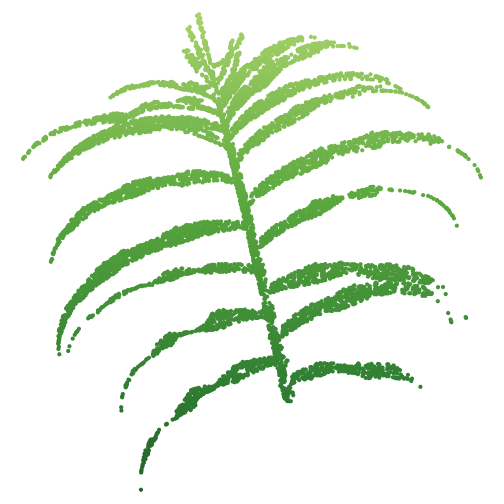
\includegraphics[width=0.8400in, height=0.8400in]{Figures/fig3/maize_pc.png}};
\draw[draw=c9D8CC4, line width=1.00pt, rounded corners=3.60pt, fill=cEAE7F2] (5.8650,1.3775) rectangle (6.7650,2.2775);
\node[anchor=south west, inner sep=0] at (5.8950,1.4075) {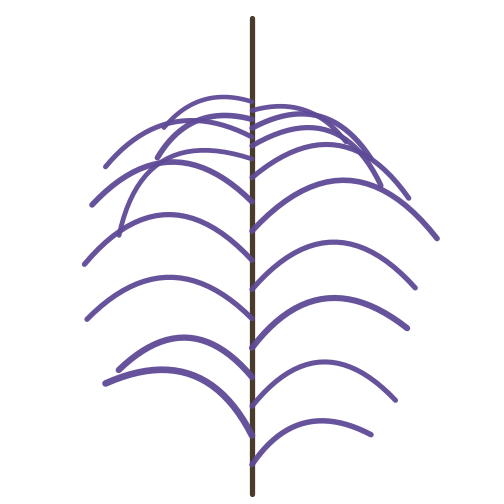
\includegraphics[width=0.8400in, height=0.8400in]{Figures/fig3/maize_text.png}};
\node[anchor=base west, inner sep=0, text=c111111, rotate=0, font={\fontsize{9.0}{10.8}\selectfont\sffamily\bfseries}] at (0.0200,1.1300) {c};
\node[anchor=base west, inner sep=0, text=c111111, rotate=0, font={\fontsize{6.2}{7.4}\selectfont\sffamily}] at (0.1800,1.1300) {Ten cameras per plant (five shown), by elevation};
\draw[draw=c809EC2, line width=1.00pt, rounded corners=2.88pt, fill=cE6ECF3] (0.2600,0.5600) rectangle (2.1800,0.9800);
\node[anchor=center, inner sep=0, text=c111111, rotate=90, font={\fontsize{5.8}{7.0}\selectfont\sffamily\bfseries}] at (0.1500,0.7700) {sorghum};
\node[anchor=south west, inner sep=0] at (0.3000,0.6000) {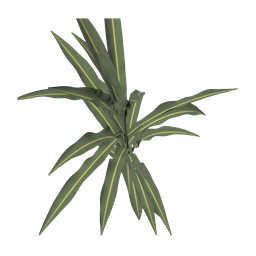
\includegraphics[width=0.3400in, height=0.3400in]{Figures/fig3/sorghum_camera_0.png}};
\node[anchor=south, inner sep=0, text=c444444, rotate=0, font={\fontsize{5.4}{6.5}\selectfont\sffamily}] at (0.4700,0.9900) {+64$^{\circ}$};
\node[anchor=south west, inner sep=0] at (0.6750,0.6000) {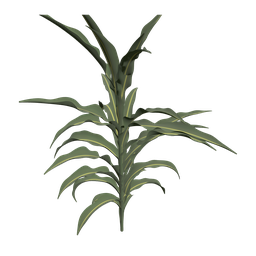
\includegraphics[width=0.3400in, height=0.3400in]{Figures/fig3/sorghum_camera_1.png}};
\node[anchor=south, inner sep=0, text=c444444, rotate=0, font={\fontsize{5.4}{6.5}\selectfont\sffamily}] at (0.8450,0.9900) {+30$^{\circ}$};
\node[anchor=south west, inner sep=0] at (1.0500,0.6000) {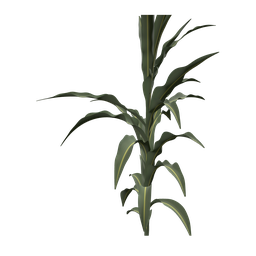
\includegraphics[width=0.3400in, height=0.3400in]{Figures/fig3/sorghum_camera_2.png}};
\node[anchor=south, inner sep=0, text=c444444, rotate=0, font={\fontsize{5.4}{6.5}\selectfont\sffamily}] at (1.2200,0.9900) {+6$^{\circ}$};
\node[anchor=south west, inner sep=0] at (1.4250,0.6000) {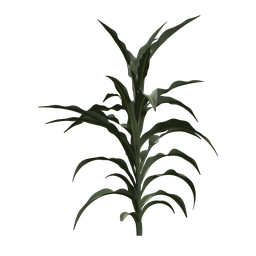
\includegraphics[width=0.3400in, height=0.3400in]{Figures/fig3/sorghum_camera_3.png}};
\node[anchor=south, inner sep=0, text=c444444, rotate=0, font={\fontsize{5.4}{6.5}\selectfont\sffamily}] at (1.5950,0.9900) {$-$17$^{\circ}$};
\node[anchor=south west, inner sep=0] at (1.8000,0.6000) {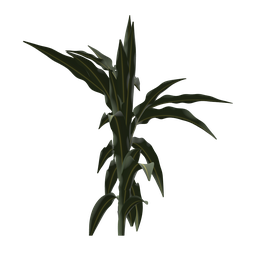
\includegraphics[width=0.3400in, height=0.3400in]{Figures/fig3/sorghum_camera_4.png}};
\node[anchor=south, inner sep=0, text=c444444, rotate=0, font={\fontsize{5.4}{6.5}\selectfont\sffamily}] at (1.9700,0.9900) {$-$44$^{\circ}$};
\draw[draw=c809EC2, line width=1.00pt, rounded corners=2.88pt, fill=cE6ECF3] (0.2600,0.0300) rectangle (2.1800,0.4500);
\node[anchor=center, inner sep=0, text=c111111, rotate=90, font={\fontsize{5.8}{7.0}\selectfont\sffamily\bfseries}] at (0.1500,0.2400) {maize};
\node[anchor=south west, inner sep=0] at (0.3000,0.0700) {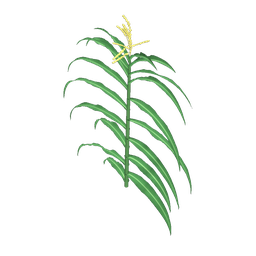
\includegraphics[width=0.3400in, height=0.3400in]{Figures/fig3/maize_camera_0.png}};
\node[anchor=south, inner sep=0, text=c444444, rotate=0, font={\fontsize{5.4}{6.5}\selectfont\sffamily}] at (0.4700,0.4600) {+39$^{\circ}$};
\node[anchor=south west, inner sep=0] at (0.6750,0.0700) {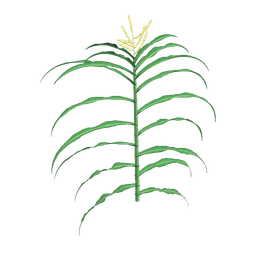
\includegraphics[width=0.3400in, height=0.3400in]{Figures/fig3/maize_camera_1.png}};
\node[anchor=south, inner sep=0, text=c444444, rotate=0, font={\fontsize{5.4}{6.5}\selectfont\sffamily}] at (0.8450,0.4600) {+30$^{\circ}$};
\node[anchor=south west, inner sep=0] at (1.0500,0.0700) {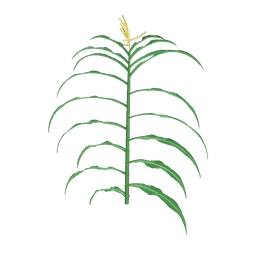
\includegraphics[width=0.3400in, height=0.3400in]{Figures/fig3/maize_camera_2.png}};
\node[anchor=south, inner sep=0, text=c444444, rotate=0, font={\fontsize{5.4}{6.5}\selectfont\sffamily}] at (1.2200,0.4600) {+10$^{\circ}$};
\node[anchor=south west, inner sep=0] at (1.4250,0.0700) {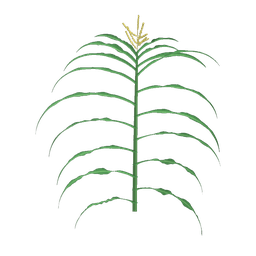
\includegraphics[width=0.3400in, height=0.3400in]{Figures/fig3/maize_camera_3.png}};
\node[anchor=south, inner sep=0, text=c444444, rotate=0, font={\fontsize{5.4}{6.5}\selectfont\sffamily}] at (1.5950,0.4600) {$-$13$^{\circ}$};
\node[anchor=south west, inner sep=0] at (1.8000,0.0700) {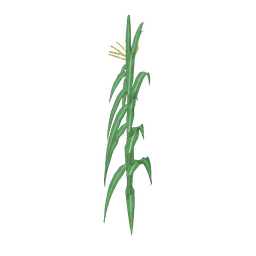
\includegraphics[width=0.3400in, height=0.3400in]{Figures/fig3/maize_camera_4.png}};
\node[anchor=south, inner sep=0, text=c444444, rotate=0, font={\fontsize{5.4}{6.5}\selectfont\sffamily}] at (1.9700,0.4600) {$-$36$^{\circ}$};
\node[anchor=base west, inner sep=0, text=c111111, rotate=0, font={\fontsize{9.0}{10.8}\selectfont\sffamily\bfseries}] at (2.8400,1.1300) {d};
\node[anchor=base west, inner sep=0, text=c111111, rotate=0, font={\fontsize{6.2}{7.4}\selectfont\sffamily}] at (3.0000,1.1300) {Crop rows: the target plant between neighbors};
\node[anchor=base west, inner sep=0, text=c555555, rotate=0, font={\fontsize{5.4}{6.5}\selectfont\sffamily}] at (3.0000,1.0250) {red: neighbor pixels;  orange: target pixels a neighbor hides (\% hidden);  green: target points};
\node[anchor=base, inner sep=0, text=c111111, rotate=0, font={\fontsize{6.2}{7.4}\selectfont\sffamily\bfseries}] at (3.7600,0.9350) {sorghum};
\draw[draw=c809EC2, line width=1.00pt, rounded corners=3.60pt, fill=cE6ECF3] (2.9900,0.1300) rectangle (3.7500,0.8900);
\node[anchor=south west, inner sep=0] at (3.0200,0.1600) {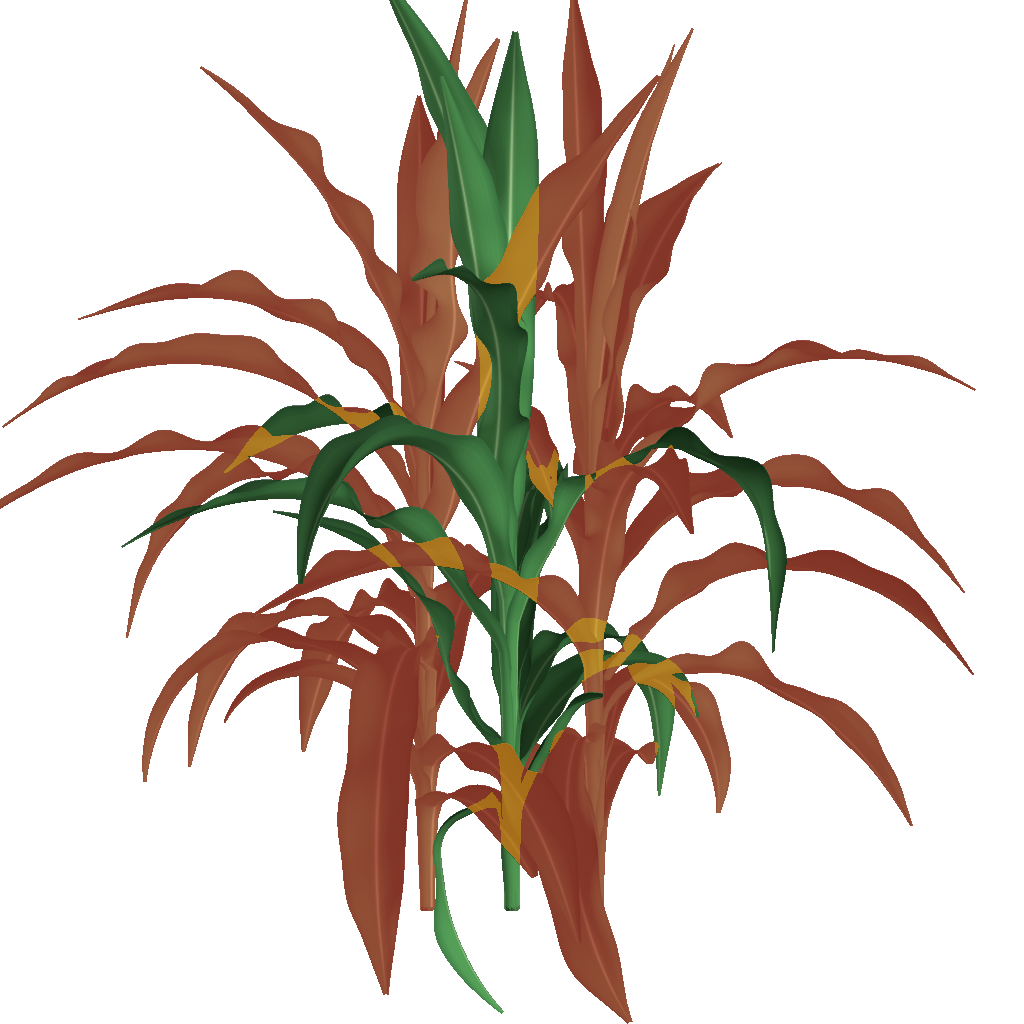
\includegraphics[width=0.7000in, height=0.7000in]{Figures/fig3/sorghum_row_image.png}};
\node[anchor=north, inner sep=0, text=c111111, rotate=0, font={\fontsize{5.6}{6.7}\selectfont\sffamily}] at (3.3700,0.1000) {16 \% hidden};
\draw[draw=cD091A7, line width=1.00pt, rounded corners=3.60pt, fill=cF6E9ED] (3.7700,0.1300) rectangle (4.5300,0.8900);
\node[anchor=south west, inner sep=0] at (3.8000,0.1600) {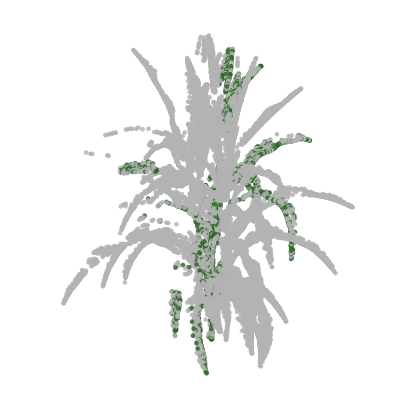
\includegraphics[width=0.7000in, height=0.7000in]{Figures/fig3/sorghum_row_cloud.png}};
\node[anchor=north, inner sep=0, text=c111111, rotate=0, font={\fontsize{5.6}{6.7}\selectfont\sffamily}] at (4.1500,0.1000) {89 \% neighbors};
\node[anchor=base, inner sep=0, text=c111111, rotate=0, font={\fontsize{6.2}{7.4}\selectfont\sffamily\bfseries}] at (5.5400,0.9350) {maize};
\draw[draw=c809EC2, line width=1.00pt, rounded corners=3.60pt, fill=cE6ECF3] (4.7700,0.1300) rectangle (5.5300,0.8900);
\node[anchor=south west, inner sep=0] at (4.8000,0.1600) {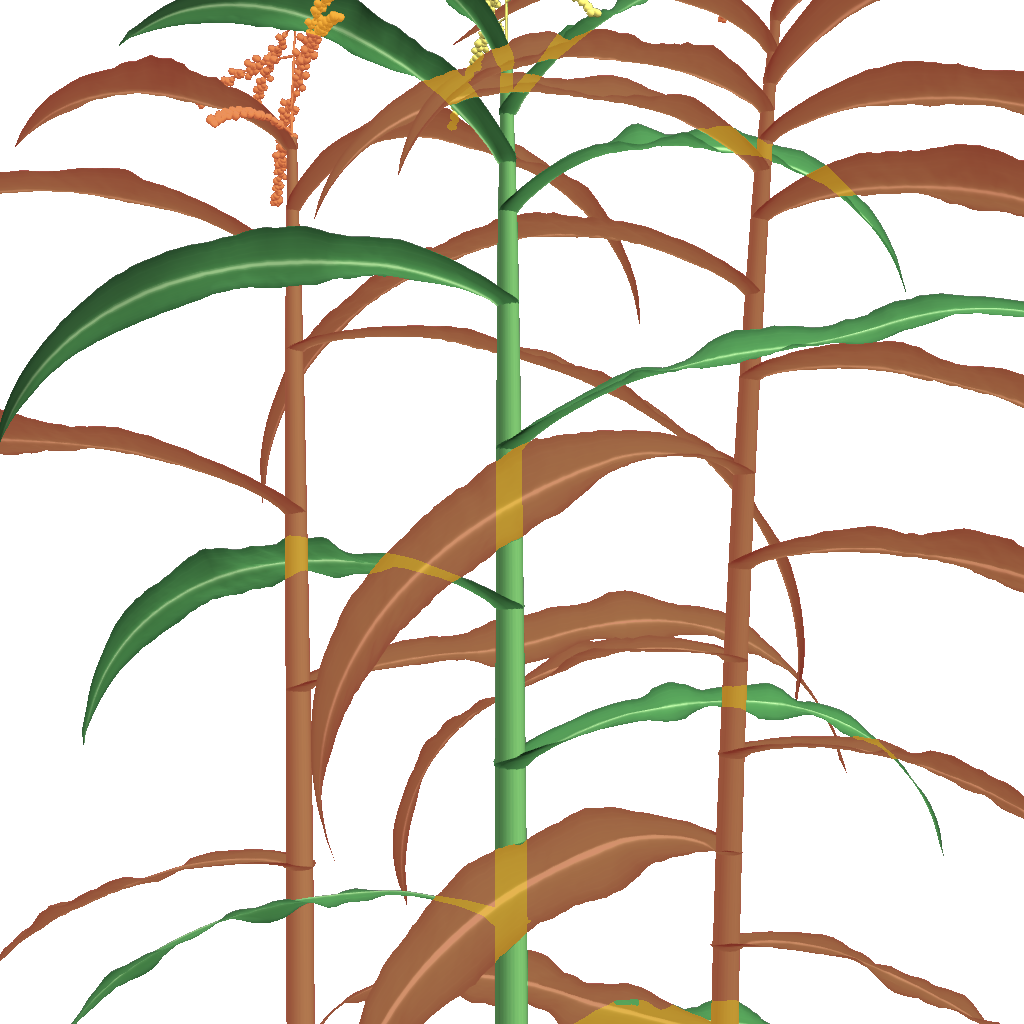
\includegraphics[width=0.7000in, height=0.7000in]{Figures/fig3/maize_row_image.png}};
\node[anchor=north, inner sep=0, text=c111111, rotate=0, font={\fontsize{5.6}{6.7}\selectfont\sffamily}] at (5.1500,0.1000) {15 \% hidden};
\draw[draw=cD091A7, line width=1.00pt, rounded corners=3.60pt, fill=cF6E9ED] (5.5500,0.1300) rectangle (6.3100,0.8900);
\node[anchor=south west, inner sep=0] at (5.5800,0.1600) {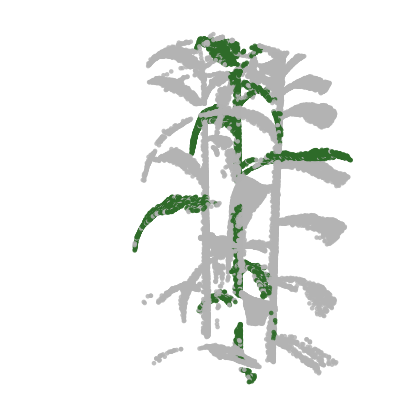
\includegraphics[width=0.7000in, height=0.7000in]{Figures/fig3/maize_row_cloud.png}};
\node[anchor=north, inner sep=0, text=c111111, rotate=0, font={\fontsize{5.6}{6.7}\selectfont\sffamily}] at (5.9300,0.1000) {75 \% neighbors};
\end{tikzpicture}
}.
\definecolor{c111111}{HTML}{111111}%
\definecolor{c333333}{HTML}{333333}%
\definecolor{c3F5F8F}{HTML}{3F5F8F}%
\definecolor{c444444}{HTML}{444444}%
\definecolor{c555555}{HTML}{555555}%
\definecolor{c5E4A96}{HTML}{5E4A96}%
\definecolor{c809EC2}{HTML}{809EC2}%
\definecolor{c9A9A9A}{HTML}{9A9A9A}%
\definecolor{c9D8CC4}{HTML}{9D8CC4}%
\definecolor{cA07800}{HTML}{A07800}%
\definecolor{cA8456E}{HTML}{A8456E}%
\definecolor{cD091A7}{HTML}{D091A7}%
\definecolor{cE0B020}{HTML}{E0B020}%
\definecolor{cE6ECF3}{HTML}{E6ECF3}%
\definecolor{cEAE7F2}{HTML}{EAE7F2}%
\definecolor{cF4F4F5}{HTML}{F4F4F5}%
\definecolor{cF6E9ED}{HTML}{F6E9ED}%
\definecolor{cFAF2D4}{HTML}{FAF2D4}%
\begin{tikzpicture}[x=1in, y=1in]
\useasboundingbox (0,0) rectangle (6.875,3.86);
\node[anchor=base west, inner sep=0, text=c111111, rotate=0, font={\fontsize{9.0}{10.8}\selectfont\sffamily\bfseries}] at (0.0200,3.7200) {a};
\node[anchor=base west, inner sep=0, text=c111111, rotate=0, font={\fontsize{6.2}{7.4}\selectfont\sffamily}] at (0.1800,3.7200) {The plants: 15,000 per species (6 shown)};
\node[anchor=base west, inner sep=0, text=c111111, rotate=0, font={\fontsize{9.0}{10.8}\selectfont\sffamily\bfseries}] at (2.3800,3.7200) {b};
\node[anchor=base west, inner sep=0, text=c111111, rotate=0, font={\fontsize{6.2}{7.4}\selectfont\sffamily}] at (2.5400,3.7200) {One view of the boxed plant as its four streams};
\draw[draw=c809EC2, line width=1.00pt, rounded corners=4.32pt, fill=cE6ECF3] (0.2400,2.4100) rectangle (1.7500,3.4450);
\node[anchor=center, inner sep=0, text=c111111, rotate=90, font={\fontsize{7.0}{8.4}\selectfont\sffamily\bfseries}] at (0.1500,2.9275) {sorghum};
\node[anchor=south west, inner sep=0] at (0.3000,2.9450) {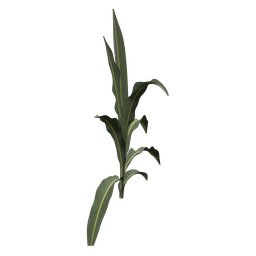
\includegraphics[width=0.4400in, height=0.4400in]{Figures/fig3/sorghum_gallery_0.png}};
\node[anchor=south west, inner sep=0] at (0.7750,2.9450) {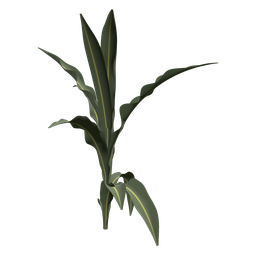
\includegraphics[width=0.4400in, height=0.4400in]{Figures/fig3/sorghum_gallery_1.png}};
\node[anchor=south west, inner sep=0] at (1.2500,2.9450) {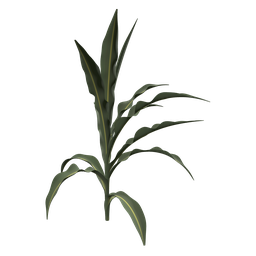
\includegraphics[width=0.4400in, height=0.4400in]{Figures/fig3/sorghum_gallery_2.png}};
\node[anchor=south west, inner sep=0] at (0.3000,2.4700) {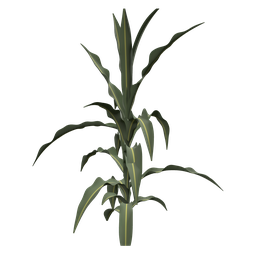
\includegraphics[width=0.4400in, height=0.4400in]{Figures/fig3/sorghum_gallery_3.png}};
\node[anchor=south west, inner sep=0] at (0.7750,2.4700) {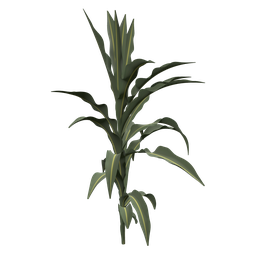
\includegraphics[width=0.4400in, height=0.4400in]{Figures/fig3/sorghum_gallery_4.png}};
\node[anchor=south west, inner sep=0] at (1.2500,2.4700) {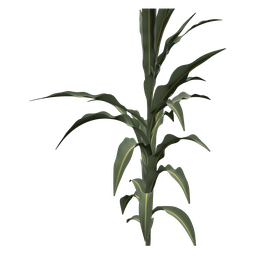
\includegraphics[width=0.4400in, height=0.4400in]{Figures/fig3/sorghum_gallery_5.png}};
\draw[draw=c333333, line width=1.00pt, rounded corners=2.16pt] (1.2350,2.4550) rectangle (1.7050,2.9250);
\draw[draw=c9A9A9A, line width=0.60pt] (1.7050,2.9250) -- (2.3700,3.4175);
\draw[draw=c9A9A9A, line width=0.60pt] (1.7050,2.4550) -- (2.3700,2.4375);
\draw[draw=c9A9A9A, line width=1.00pt, rounded corners=4.32pt, fill=cF4F4F5] (2.3700,2.4375) rectangle (6.8050,3.4175);
\draw[draw=c809EC2, line width=1.00pt, rounded corners=3.60pt, fill=cE6ECF3] (2.4100,2.4775) rectangle (3.3100,3.3775);
\node[anchor=south west, inner sep=0] at (2.4400,2.5075) {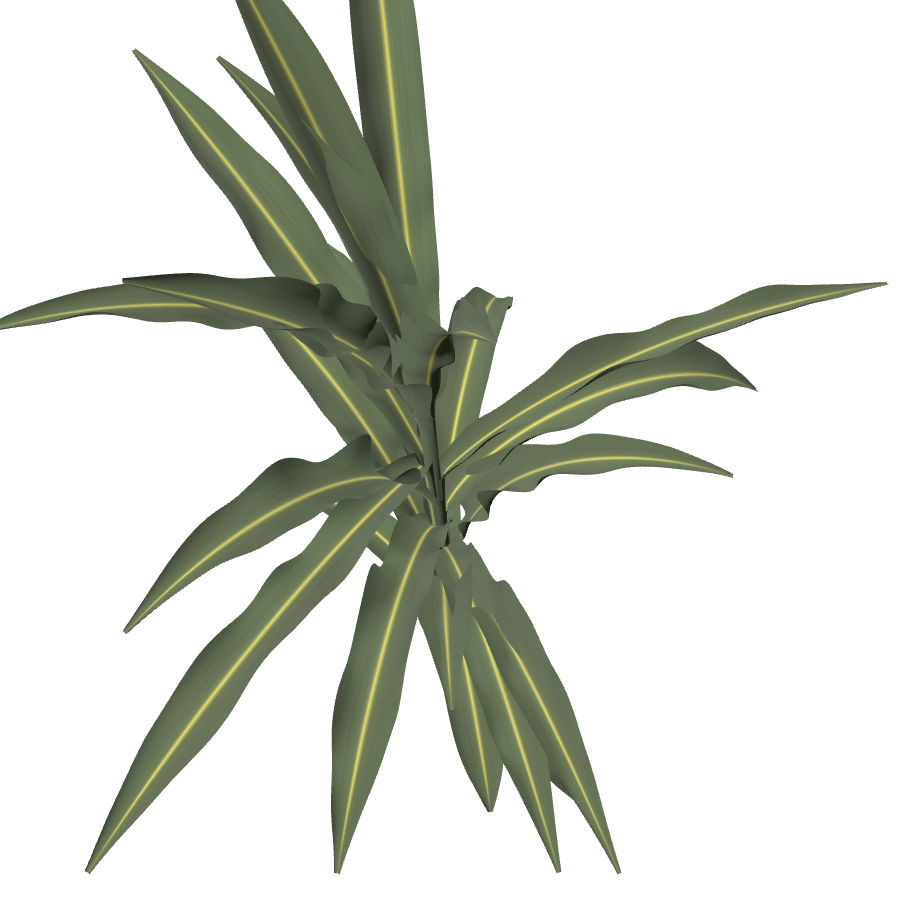
\includegraphics[width=0.8400in, height=0.8400in]{Figures/fig3/sorghum_rgb.png}};
\node[anchor=base, inner sep=0, text=c3F5F8F, rotate=0, font={\fontsize{6.2}{7.4}\selectfont\sffamily\bfseries}] at (2.8600,3.4925) {Image};
\draw[draw=cE0B020, line width=1.00pt, rounded corners=3.60pt, fill=cFAF2D4] (3.5617,2.4775) rectangle (4.4617,3.3775);
\node[anchor=south west, inner sep=0] at (3.5917,2.5075) {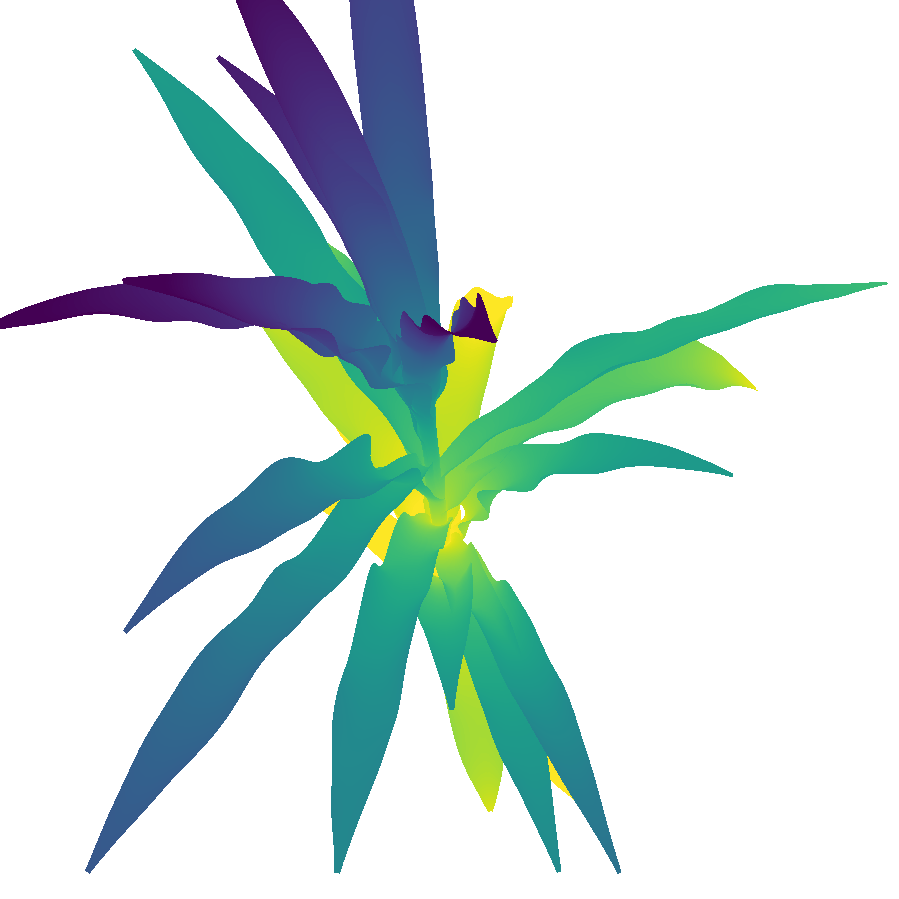
\includegraphics[width=0.8400in, height=0.8400in]{Figures/fig3/sorghum_depth.png}};
\node[anchor=base, inner sep=0, text=cA07800, rotate=0, font={\fontsize{6.2}{7.4}\selectfont\sffamily\bfseries}] at (4.0117,3.4925) {Depth image};
\draw[draw=cD091A7, line width=1.00pt, rounded corners=3.60pt, fill=cF6E9ED] (4.7133,2.4775) rectangle (5.6133,3.3775);
\node[anchor=south west, inner sep=0] at (4.7433,2.5075) {
\includegraphics[width=0.8400in, height=0.8400in]{Figures/fig3/sorghum_pc.png}};
\node[anchor=base, inner sep=0, text=cA8456E, rotate=0, font={\fontsize{6.2}{7.4}\selectfont\sffamily\bfseries}] at (5.1633,3.4925) {Point cloud};
\draw[draw=c9D8CC4, line width=1.00pt, rounded corners=3.60pt, fill=cEAE7F2] (5.8650,2.4775) rectangle (6.7650,3.3775);
\node[anchor=south west, inner sep=0] at (5.8950,2.5075) {
\includegraphics[width=0.8400in, height=0.8400in]{Figures/fig3/sorghum_text.png}};
\node[anchor=base, inner sep=0, text=c5E4A96, rotate=0, font={\fontsize{6.2}{7.4}\selectfont\sffamily\bfseries}] at (6.3150,3.4925) {Procedural parameters};
\draw[draw=c809EC2, line width=1.00pt, rounded corners=4.32pt, fill=cE6ECF3] (0.2400,1.3100) rectangle (1.7500,2.3450);
\node[anchor=center, inner sep=0, text=c111111, rotate=90, font={\fontsize{7.0}{8.4}\selectfont\sffamily\bfseries}] at (0.1500,1.8275) {maize};
\node[anchor=south west, inner sep=0] at (0.3000,1.8450) {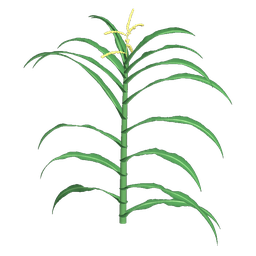
\includegraphics[width=0.4400in, height=0.4400in]{Figures/fig3/maize_gallery_0.png}};
\node[anchor=south west, inner sep=0] at (0.7750,1.8450) {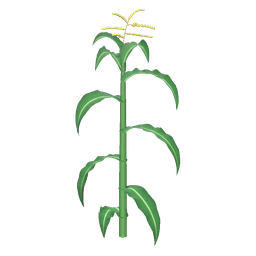
\includegraphics[width=0.4400in, height=0.4400in]{Figures/fig3/maize_gallery_1.png}};
\node[anchor=south west, inner sep=0] at (1.2500,1.8450) {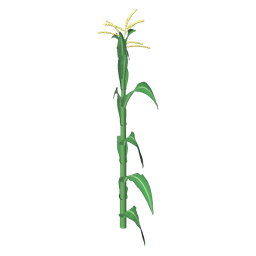
\includegraphics[width=0.4400in, height=0.4400in]{Figures/fig3/maize_gallery_2.png}};
\node[anchor=south west, inner sep=0] at (0.3000,1.3700) {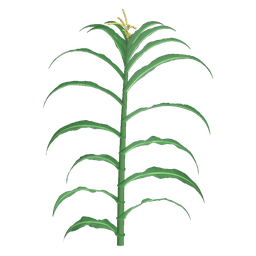
\includegraphics[width=0.4400in, height=0.4400in]{Figures/fig3/maize_gallery_3.png}};
\node[anchor=south west, inner sep=0] at (0.7750,1.3700) {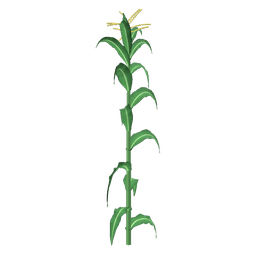
\includegraphics[width=0.4400in, height=0.4400in]{Figures/fig3/maize_gallery_4.png}};
\node[anchor=south west, inner sep=0] at (1.2500,1.3700) {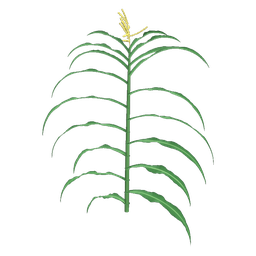
\includegraphics[width=0.4400in, height=0.4400in]{Figures/fig3/maize_gallery_5.png}};
\draw[draw=c333333, line width=1.00pt, rounded corners=2.16pt] (1.2350,1.3550) rectangle (1.7050,1.8250);
\draw[draw=c9A9A9A, line width=0.60pt] (1.7050,1.8250) -- (2.3700,2.3175);
\draw[draw=c9A9A9A, line width=0.60pt] (1.7050,1.3550) -- (2.3700,1.3375);
\draw[draw=c9A9A9A, line width=1.00pt, rounded corners=4.32pt, fill=cF4F4F5] (2.3700,1.3375) rectangle (6.8050,2.3175);
\draw[draw=c809EC2, line width=1.00pt, rounded corners=3.60pt, fill=cE6ECF3] (2.4100,1.3775) rectangle (3.3100,2.2775);
\node[anchor=south west, inner sep=0] at (2.4400,1.4075) {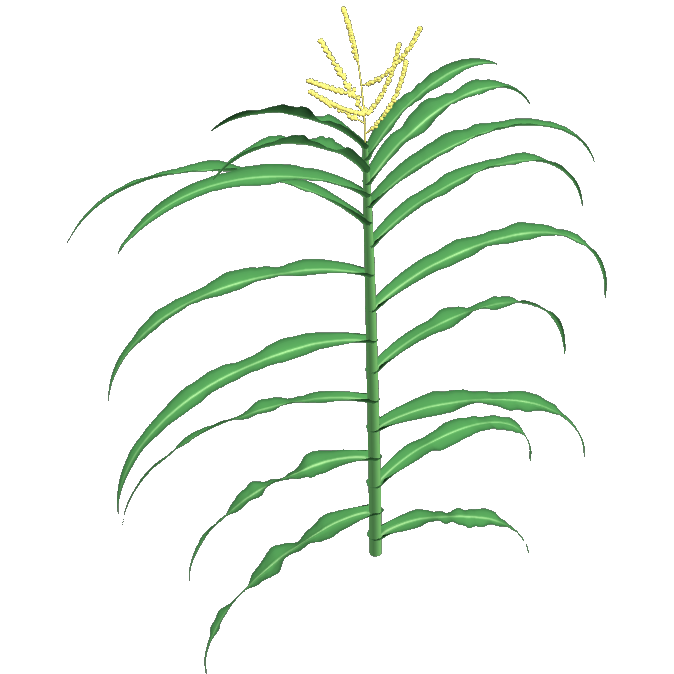
\includegraphics[width=0.8400in, height=0.8400in]{Figures/fig3/maize_rgb.png}};
\draw[draw=cE0B020, line width=1.00pt, rounded corners=3.60pt, fill=cFAF2D4] (3.5617,1.3775) rectangle (4.4617,2.2775);
\node[anchor=south west, inner sep=0] at (3.5917,1.4075) {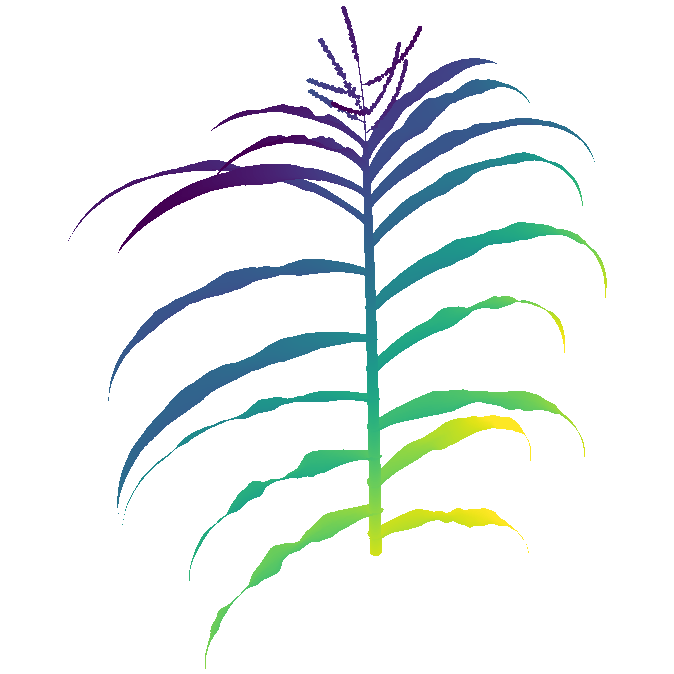
\includegraphics[width=0.8400in, height=0.8400in]{Figures/fig3/maize_depth.png}};
\draw[draw=cD091A7, line width=1.00pt, rounded corners=3.60pt, fill=cF6E9ED] (4.7133,1.3775) rectangle (5.6133,2.2775);
\node[anchor=south west, inner sep=0] at (4.7433,1.4075) {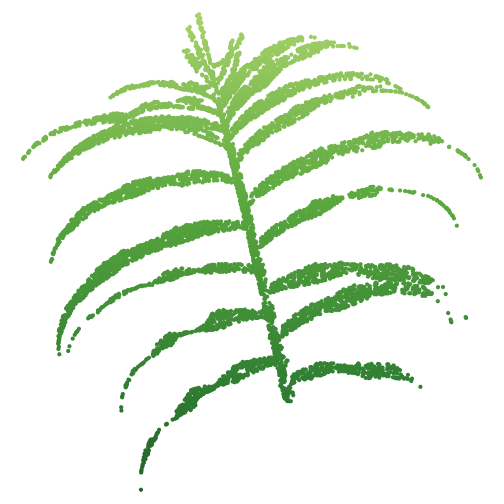
\includegraphics[width=0.8400in, height=0.8400in]{Figures/fig3/maize_pc.png}};
\draw[draw=c9D8CC4, line width=1.00pt, rounded corners=3.60pt, fill=cEAE7F2] (5.8650,1.3775) rectangle (6.7650,2.2775);
\node[anchor=south west, inner sep=0] at (5.8950,1.4075) {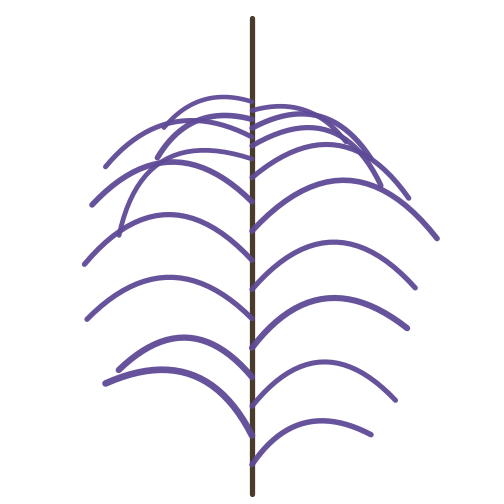
\includegraphics[width=0.8400in, height=0.8400in]{Figures/fig3/maize_text.png}};
\node[anchor=base west, inner sep=0, text=c111111, rotate=0, font={\fontsize{9.0}{10.8}\selectfont\sffamily\bfseries}] at (0.0200,1.1300) {c};
\node[anchor=base west, inner sep=0, text=c111111, rotate=0, font={\fontsize{6.2}{7.4}\selectfont\sffamily}] at (0.1800,1.1300) {Ten cameras per plant (five shown), by elevation};
\draw[draw=c809EC2, line width=1.00pt, rounded corners=2.88pt, fill=cE6ECF3] (0.2600,0.5600) rectangle (2.1800,0.9800);
\node[anchor=center, inner sep=0, text=c111111, rotate=90, font={\fontsize{5.8}{7.0}\selectfont\sffamily\bfseries}] at (0.1500,0.7700) {sorghum};
\node[anchor=south west, inner sep=0] at (0.3000,0.6000) {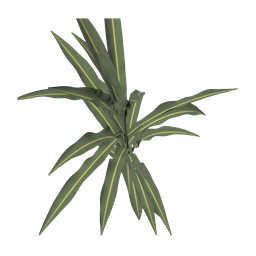
\includegraphics[width=0.3400in, height=0.3400in]{Figures/fig3/sorghum_camera_0.png}};
\node[anchor=south, inner sep=0, text=c444444, rotate=0, font={\fontsize{5.4}{6.5}\selectfont\sffamily}] at (0.4700,0.9900) {+64$^{\circ}$};
\node[anchor=south west, inner sep=0] at (0.6750,0.6000) {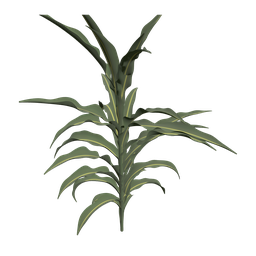
\includegraphics[width=0.3400in, height=0.3400in]{Figures/fig3/sorghum_camera_1.png}};
\node[anchor=south, inner sep=0, text=c444444, rotate=0, font={\fontsize{5.4}{6.5}\selectfont\sffamily}] at (0.8450,0.9900) {+30$^{\circ}$};
\node[anchor=south west, inner sep=0] at (1.0500,0.6000) {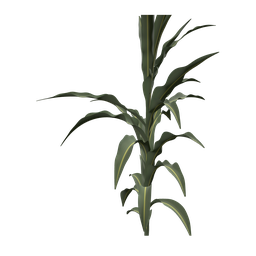
\includegraphics[width=0.3400in, height=0.3400in]{Figures/fig3/sorghum_camera_2.png}};
\node[anchor=south, inner sep=0, text=c444444, rotate=0, font={\fontsize{5.4}{6.5}\selectfont\sffamily}] at (1.2200,0.9900) {+6$^{\circ}$};
\node[anchor=south west, inner sep=0] at (1.4250,0.6000) {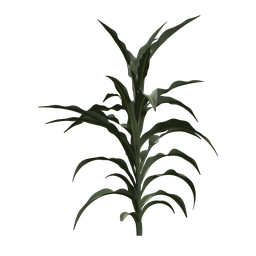
\includegraphics[width=0.3400in, height=0.3400in]{Figures/fig3/sorghum_camera_3.png}};
\node[anchor=south, inner sep=0, text=c444444, rotate=0, font={\fontsize{5.4}{6.5}\selectfont\sffamily}] at (1.5950,0.9900) {$-$17$^{\circ}$};
\node[anchor=south west, inner sep=0] at (1.8000,0.6000) {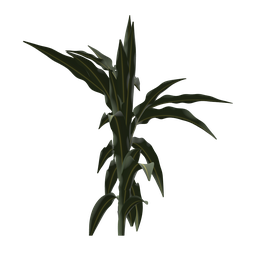
\includegraphics[width=0.3400in, height=0.3400in]{Figures/fig3/sorghum_camera_4.png}};
\node[anchor=south, inner sep=0, text=c444444, rotate=0, font={\fontsize{5.4}{6.5}\selectfont\sffamily}] at (1.9700,0.9900) {$-$44$^{\circ}$};
\draw[draw=c809EC2, line width=1.00pt, rounded corners=2.88pt, fill=cE6ECF3] (0.2600,0.0300) rectangle (2.1800,0.4500);
\node[anchor=center, inner sep=0, text=c111111, rotate=90, font={\fontsize{5.8}{7.0}\selectfont\sffamily\bfseries}] at (0.1500,0.2400) {maize};
\node[anchor=south west, inner sep=0] at (0.3000,0.0700) {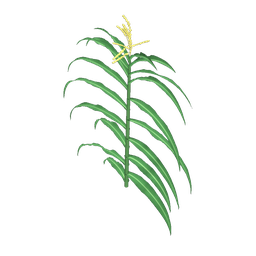
\includegraphics[width=0.3400in, height=0.3400in]{Figures/fig3/maize_camera_0.png}};
\node[anchor=south, inner sep=0, text=c444444, rotate=0, font={\fontsize{5.4}{6.5}\selectfont\sffamily}] at (0.4700,0.4600) {+39$^{\circ}$};
\node[anchor=south west, inner sep=0] at (0.6750,0.0700) {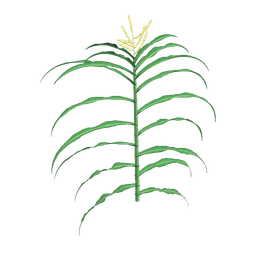
\includegraphics[width=0.3400in, height=0.3400in]{Figures/fig3/maize_camera_1.png}};
\node[anchor=south, inner sep=0, text=c444444, rotate=0, font={\fontsize{5.4}{6.5}\selectfont\sffamily}] at (0.8450,0.4600) {+30$^{\circ}$};
\node[anchor=south west, inner sep=0] at (1.0500,0.0700) {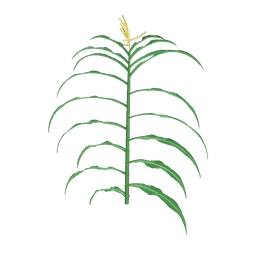
\includegraphics[width=0.3400in, height=0.3400in]{Figures/fig3/maize_camera_2.png}};
\node[anchor=south, inner sep=0, text=c444444, rotate=0, font={\fontsize{5.4}{6.5}\selectfont\sffamily}] at (1.2200,0.4600) {+10$^{\circ}$};
\node[anchor=south west, inner sep=0] at (1.4250,0.0700) {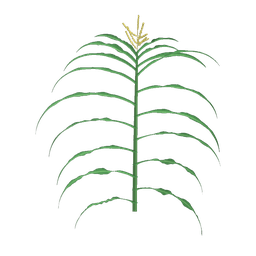
\includegraphics[width=0.3400in, height=0.3400in]{Figures/fig3/maize_camera_3.png}};
\node[anchor=south, inner sep=0, text=c444444, rotate=0, font={\fontsize{5.4}{6.5}\selectfont\sffamily}] at (1.5950,0.4600) {$-$13$^{\circ}$};
\node[anchor=south west, inner sep=0] at (1.8000,0.0700) {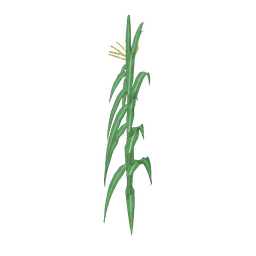
\includegraphics[width=0.3400in, height=0.3400in]{Figures/fig3/maize_camera_4.png}};
\node[anchor=south, inner sep=0, text=c444444, rotate=0, font={\fontsize{5.4}{6.5}\selectfont\sffamily}] at (1.9700,0.4600) {$-$36$^{\circ}$};
\node[anchor=base west, inner sep=0, text=c111111, rotate=0, font={\fontsize{9.0}{10.8}\selectfont\sffamily\bfseries}] at (2.8400,1.1300) {d};
\node[anchor=base west, inner sep=0, text=c111111, rotate=0, font={\fontsize{6.2}{7.4}\selectfont\sffamily}] at (3.0000,1.1300) {Crop rows: the target plant between neighbors};
\node[anchor=base west, inner sep=0, text=c555555, rotate=0, font={\fontsize{5.4}{6.5}\selectfont\sffamily}] at (3.0000,1.0250) {red: neighbor pixels;  orange: target pixels a neighbor hides (\% hidden);  green: target points};
\node[anchor=base, inner sep=0, text=c111111, rotate=0, font={\fontsize{6.2}{7.4}\selectfont\sffamily\bfseries}] at (3.7600,0.9350) {sorghum};
\draw[draw=c809EC2, line width=1.00pt, rounded corners=3.60pt, fill=cE6ECF3] (2.9900,0.1300) rectangle (3.7500,0.8900);
\node[anchor=south west, inner sep=0] at (3.0200,0.1600) {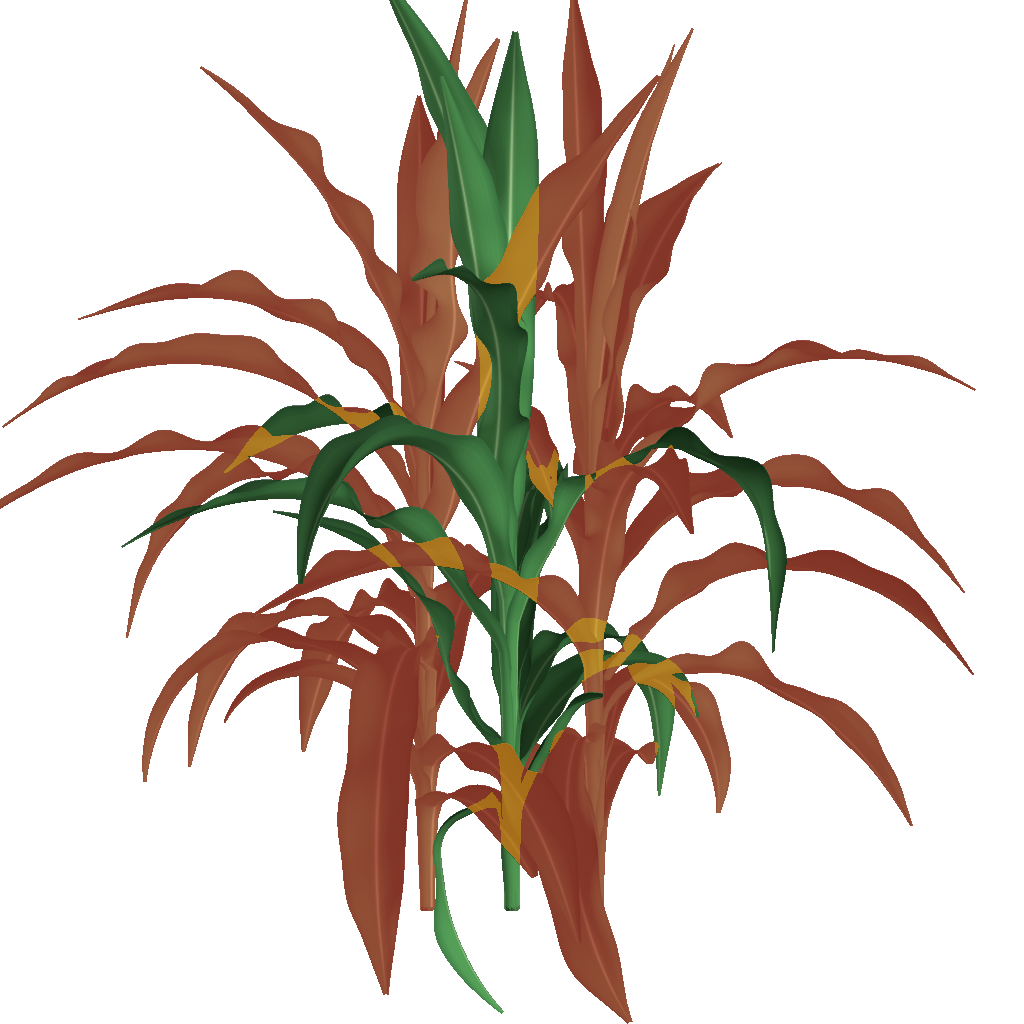
\includegraphics[width=0.7000in, height=0.7000in]{Figures/fig3/sorghum_row_image.png}};
\node[anchor=north, inner sep=0, text=c111111, rotate=0, font={\fontsize{5.6}{6.7}\selectfont\sffamily}] at (3.3700,0.1000) {16 \% hidden};
\draw[draw=cD091A7, line width=1.00pt, rounded corners=3.60pt, fill=cF6E9ED] (3.7700,0.1300) rectangle (4.5300,0.8900);
\node[anchor=south west, inner sep=0] at (3.8000,0.1600) {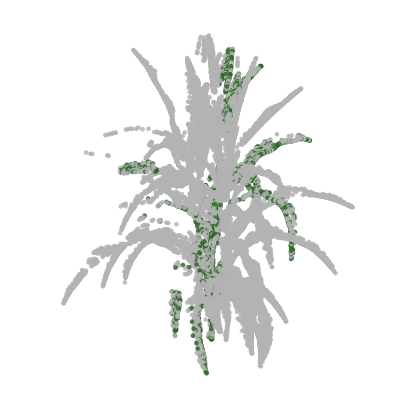
\includegraphics[width=0.7000in, height=0.7000in]{Figures/fig3/sorghum_row_cloud.png}};
\node[anchor=north, inner sep=0, text=c111111, rotate=0, font={\fontsize{5.6}{6.7}\selectfont\sffamily}] at (4.1500,0.1000) {89 \% neighbors};
\node[anchor=base, inner sep=0, text=c111111, rotate=0, font={\fontsize{6.2}{7.4}\selectfont\sffamily\bfseries}] at (5.5400,0.9350) {maize};
\draw[draw=c809EC2, line width=1.00pt, rounded corners=3.60pt, fill=cE6ECF3] (4.7700,0.1300) rectangle (5.5300,0.8900);
\node[anchor=south west, inner sep=0] at (4.8000,0.1600) {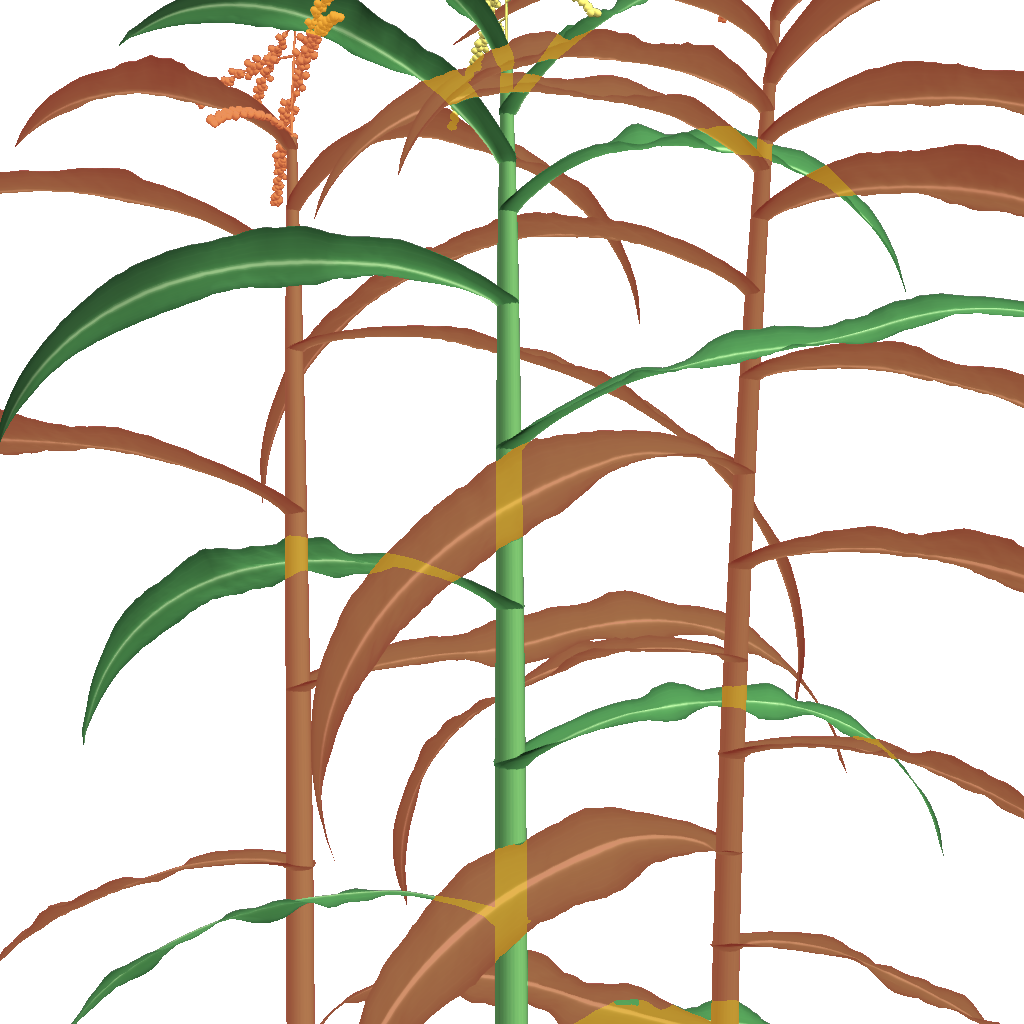
\includegraphics[width=0.7000in, height=0.7000in]{Figures/fig3/maize_row_image.png}};
\node[anchor=north, inner sep=0, text=c111111, rotate=0, font={\fontsize{5.6}{6.7}\selectfont\sffamily}] at (5.1500,0.1000) {15 \% hidden};
\draw[draw=cD091A7, line width=1.00pt, rounded corners=3.60pt, fill=cF6E9ED] (5.5500,0.1300) rectangle (6.3100,0.8900);
\node[anchor=south west, inner sep=0] at (5.5800,0.1600) {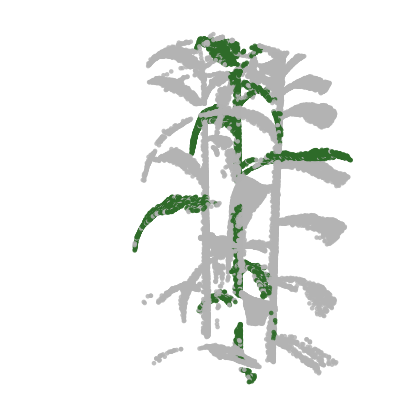
\includegraphics[width=0.7000in, height=0.7000in]{Figures/fig3/maize_row_cloud.png}};
\node[anchor=north, inner sep=0, text=c111111, rotate=0, font={\fontsize{5.6}{6.7}\selectfont\sffamily}] at (5.9300,0.1000) {75 \% neighbors};
\end{tikzpicture}
}.
\definecolor{c111111}{HTML}{111111}%
\definecolor{c333333}{HTML}{333333}%
\definecolor{c3F5F8F}{HTML}{3F5F8F}%
\definecolor{c444444}{HTML}{444444}%
\definecolor{c555555}{HTML}{555555}%
\definecolor{c5E4A96}{HTML}{5E4A96}%
\definecolor{c809EC2}{HTML}{809EC2}%
\definecolor{c9A9A9A}{HTML}{9A9A9A}%
\definecolor{c9D8CC4}{HTML}{9D8CC4}%
\definecolor{cA07800}{HTML}{A07800}%
\definecolor{cA8456E}{HTML}{A8456E}%
\definecolor{cD091A7}{HTML}{D091A7}%
\definecolor{cE0B020}{HTML}{E0B020}%
\definecolor{cE6ECF3}{HTML}{E6ECF3}%
\definecolor{cEAE7F2}{HTML}{EAE7F2}%
\definecolor{cF4F4F5}{HTML}{F4F4F5}%
\definecolor{cF6E9ED}{HTML}{F6E9ED}%
\definecolor{cFAF2D4}{HTML}{FAF2D4}%
\begin{tikzpicture}[x=1in, y=1in]
\useasboundingbox (0,0) rectangle (6.875,3.86);
\node[anchor=base west, inner sep=0, text=c111111, rotate=0, font={\fontsize{9.0}{10.8}\selectfont\sffamily\bfseries}] at (0.0200,3.7200) {a};
\node[anchor=base west, inner sep=0, text=c111111, rotate=0, font={\fontsize{6.2}{7.4}\selectfont\sffamily}] at (0.1800,3.7200) {The plants: 15,000 per species (6 shown)};
\node[anchor=base west, inner sep=0, text=c111111, rotate=0, font={\fontsize{9.0}{10.8}\selectfont\sffamily\bfseries}] at (2.3800,3.7200) {b};
\node[anchor=base west, inner sep=0, text=c111111, rotate=0, font={\fontsize{6.2}{7.4}\selectfont\sffamily}] at (2.5400,3.7200) {One view of the boxed plant as its four streams};
\draw[draw=c809EC2, line width=1.00pt, rounded corners=4.32pt, fill=cE6ECF3] (0.2400,2.4100) rectangle (1.7500,3.4450);
\node[anchor=center, inner sep=0, text=c111111, rotate=90, font={\fontsize{7.0}{8.4}\selectfont\sffamily\bfseries}] at (0.1500,2.9275) {sorghum};
\node[anchor=south west, inner sep=0] at (0.3000,2.9450) {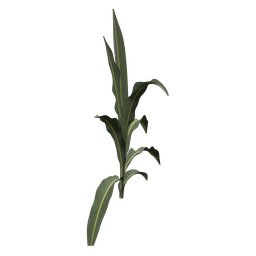
\includegraphics[width=0.4400in, height=0.4400in]{Figures/fig3/sorghum_gallery_0.png}};
\node[anchor=south west, inner sep=0] at (0.7750,2.9450) {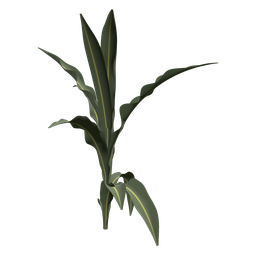
\includegraphics[width=0.4400in, height=0.4400in]{Figures/fig3/sorghum_gallery_1.png}};
\node[anchor=south west, inner sep=0] at (1.2500,2.9450) {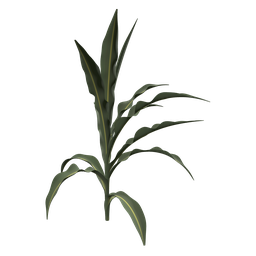
\includegraphics[width=0.4400in, height=0.4400in]{Figures/fig3/sorghum_gallery_2.png}};
\node[anchor=south west, inner sep=0] at (0.3000,2.4700) {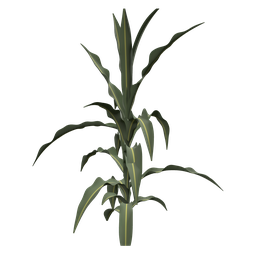
\includegraphics[width=0.4400in, height=0.4400in]{Figures/fig3/sorghum_gallery_3.png}};
\node[anchor=south west, inner sep=0] at (0.7750,2.4700) {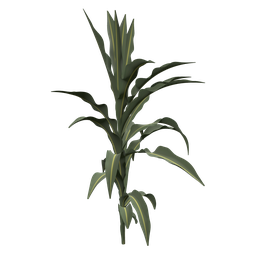
\includegraphics[width=0.4400in, height=0.4400in]{Figures/fig3/sorghum_gallery_4.png}};
\node[anchor=south west, inner sep=0] at (1.2500,2.4700) {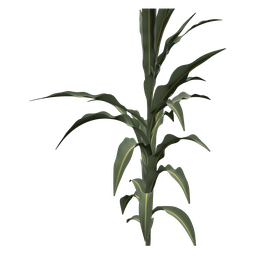
\includegraphics[width=0.4400in, height=0.4400in]{Figures/fig3/sorghum_gallery_5.png}};
\draw[draw=c333333, line width=1.00pt, rounded corners=2.16pt] (1.2350,2.4550) rectangle (1.7050,2.9250);
\draw[draw=c9A9A9A, line width=0.60pt] (1.7050,2.9250) -- (2.3700,3.4175);
\draw[draw=c9A9A9A, line width=0.60pt] (1.7050,2.4550) -- (2.3700,2.4375);
\draw[draw=c9A9A9A, line width=1.00pt, rounded corners=4.32pt, fill=cF4F4F5] (2.3700,2.4375) rectangle (6.8050,3.4175);
\draw[draw=c809EC2, line width=1.00pt, rounded corners=3.60pt, fill=cE6ECF3] (2.4100,2.4775) rectangle (3.3100,3.3775);
\node[anchor=south west, inner sep=0] at (2.4400,2.5075) {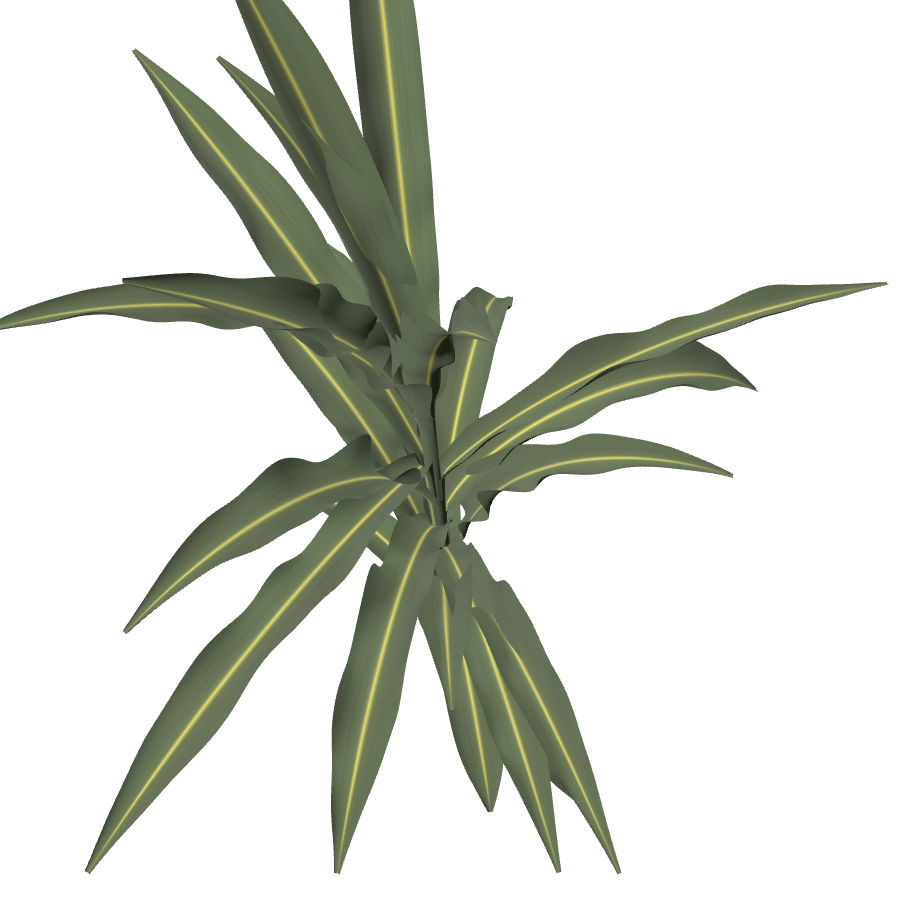
\includegraphics[width=0.8400in, height=0.8400in]{Figures/fig3/sorghum_rgb.png}};
\node[anchor=base, inner sep=0, text=c3F5F8F, rotate=0, font={\fontsize{6.2}{7.4}\selectfont\sffamily\bfseries}] at (2.8600,3.4925) {Image};
\draw[draw=cE0B020, line width=1.00pt, rounded corners=3.60pt, fill=cFAF2D4] (3.5617,2.4775) rectangle (4.4617,3.3775);
\node[anchor=south west, inner sep=0] at (3.5917,2.5075) {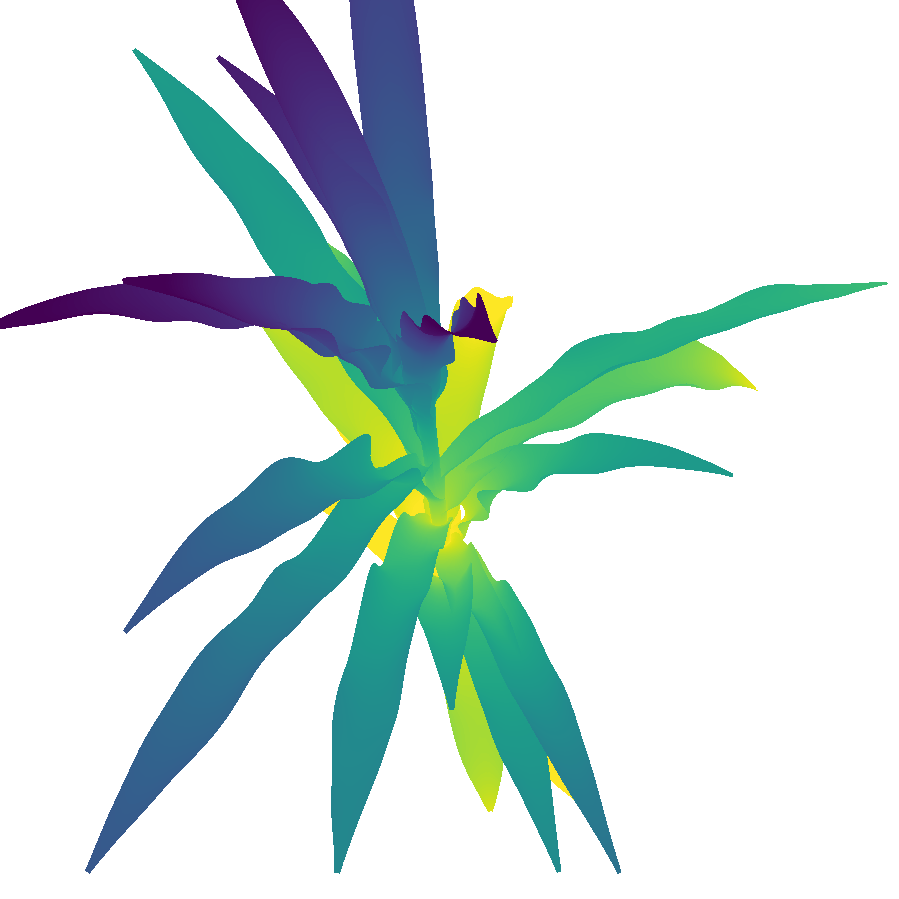
\includegraphics[width=0.8400in, height=0.8400in]{Figures/fig3/sorghum_depth.png}};
\node[anchor=base, inner sep=0, text=cA07800, rotate=0, font={\fontsize{6.2}{7.4}\selectfont\sffamily\bfseries}] at (4.0117,3.4925) {Depth image};
\draw[draw=cD091A7, line width=1.00pt, rounded corners=3.60pt, fill=cF6E9ED] (4.7133,2.4775) rectangle (5.6133,3.3775);
\node[anchor=south west, inner sep=0] at (4.7433,2.5075) {
\includegraphics[width=0.8400in, height=0.8400in]{Figures/fig3/sorghum_pc.png}};
\node[anchor=base, inner sep=0, text=cA8456E, rotate=0, font={\fontsize{6.2}{7.4}\selectfont\sffamily\bfseries}] at (5.1633,3.4925) {Point cloud};
\draw[draw=c9D8CC4, line width=1.00pt, rounded corners=3.60pt, fill=cEAE7F2] (5.8650,2.4775) rectangle (6.7650,3.3775);
\node[anchor=south west, inner sep=0] at (5.8950,2.5075) {
\includegraphics[width=0.8400in, height=0.8400in]{Figures/fig3/sorghum_text.png}};
\node[anchor=base, inner sep=0, text=c5E4A96, rotate=0, font={\fontsize{6.2}{7.4}\selectfont\sffamily\bfseries}] at (6.3150,3.4925) {Procedural parameters};
\draw[draw=c809EC2, line width=1.00pt, rounded corners=4.32pt, fill=cE6ECF3] (0.2400,1.3100) rectangle (1.7500,2.3450);
\node[anchor=center, inner sep=0, text=c111111, rotate=90, font={\fontsize{7.0}{8.4}\selectfont\sffamily\bfseries}] at (0.1500,1.8275) {maize};
\node[anchor=south west, inner sep=0] at (0.3000,1.8450) {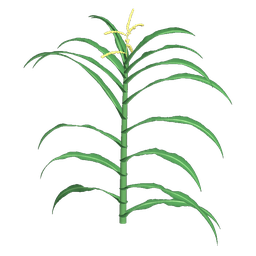
\includegraphics[width=0.4400in, height=0.4400in]{Figures/fig3/maize_gallery_0.png}};
\node[anchor=south west, inner sep=0] at (0.7750,1.8450) {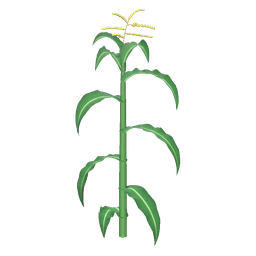
\includegraphics[width=0.4400in, height=0.4400in]{Figures/fig3/maize_gallery_1.png}};
\node[anchor=south west, inner sep=0] at (1.2500,1.8450) {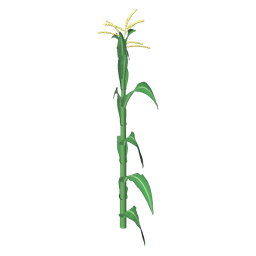
\includegraphics[width=0.4400in, height=0.4400in]{Figures/fig3/maize_gallery_2.png}};
\node[anchor=south west, inner sep=0] at (0.3000,1.3700) {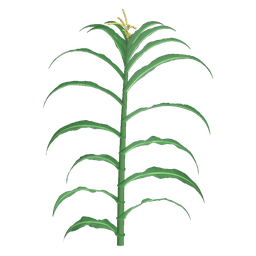
\includegraphics[width=0.4400in, height=0.4400in]{Figures/fig3/maize_gallery_3.png}};
\node[anchor=south west, inner sep=0] at (0.7750,1.3700) {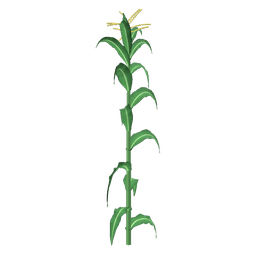
\includegraphics[width=0.4400in, height=0.4400in]{Figures/fig3/maize_gallery_4.png}};
\node[anchor=south west, inner sep=0] at (1.2500,1.3700) {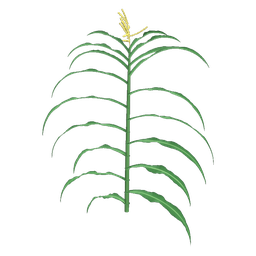
\includegraphics[width=0.4400in, height=0.4400in]{Figures/fig3/maize_gallery_5.png}};
\draw[draw=c333333, line width=1.00pt, rounded corners=2.16pt] (1.2350,1.3550) rectangle (1.7050,1.8250);
\draw[draw=c9A9A9A, line width=0.60pt] (1.7050,1.8250) -- (2.3700,2.3175);
\draw[draw=c9A9A9A, line width=0.60pt] (1.7050,1.3550) -- (2.3700,1.3375);
\draw[draw=c9A9A9A, line width=1.00pt, rounded corners=4.32pt, fill=cF4F4F5] (2.3700,1.3375) rectangle (6.8050,2.3175);
\draw[draw=c809EC2, line width=1.00pt, rounded corners=3.60pt, fill=cE6ECF3] (2.4100,1.3775) rectangle (3.3100,2.2775);
\node[anchor=south west, inner sep=0] at (2.4400,1.4075) {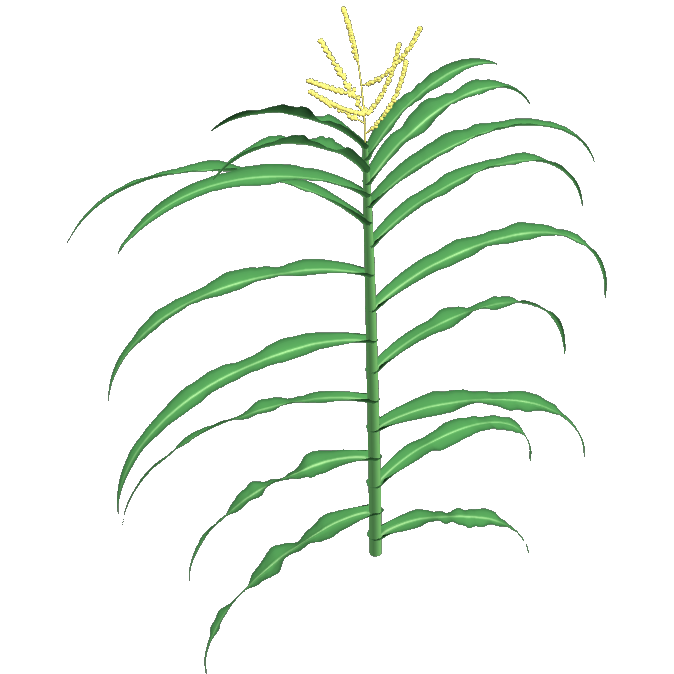
\includegraphics[width=0.8400in, height=0.8400in]{Figures/fig3/maize_rgb.png}};
\draw[draw=cE0B020, line width=1.00pt, rounded corners=3.60pt, fill=cFAF2D4] (3.5617,1.3775) rectangle (4.4617,2.2775);
\node[anchor=south west, inner sep=0] at (3.5917,1.4075) {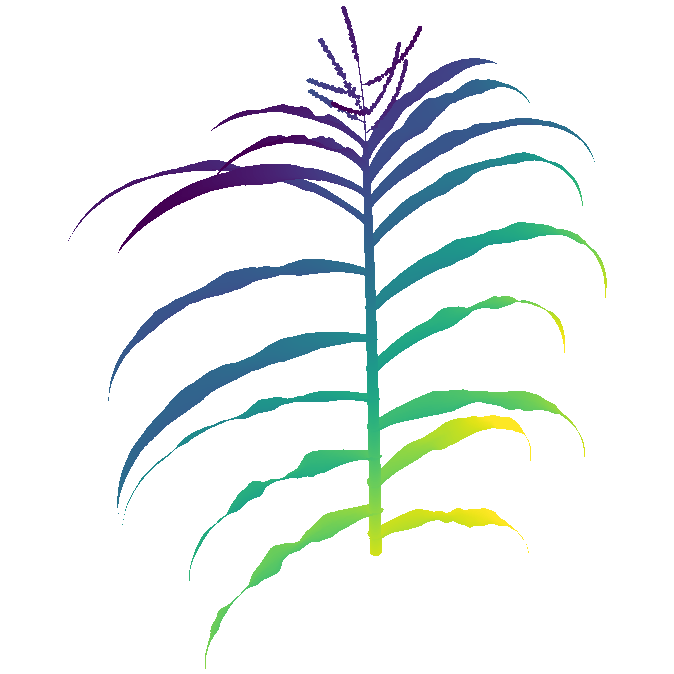
\includegraphics[width=0.8400in, height=0.8400in]{Figures/fig3/maize_depth.png}};
\draw[draw=cD091A7, line width=1.00pt, rounded corners=3.60pt, fill=cF6E9ED] (4.7133,1.3775) rectangle (5.6133,2.2775);
\node[anchor=south west, inner sep=0] at (4.7433,1.4075) {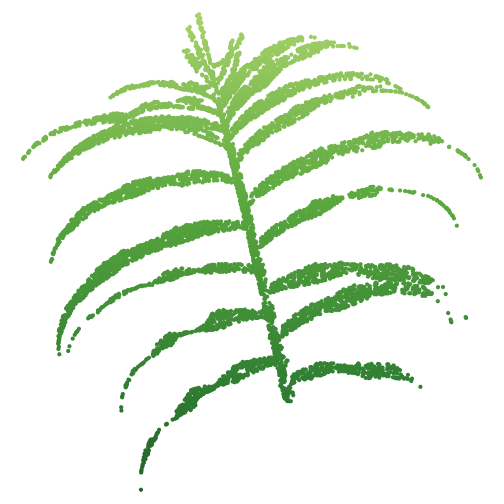
\includegraphics[width=0.8400in, height=0.8400in]{Figures/fig3/maize_pc.png}};
\draw[draw=c9D8CC4, line width=1.00pt, rounded corners=3.60pt, fill=cEAE7F2] (5.8650,1.3775) rectangle (6.7650,2.2775);
\node[anchor=south west, inner sep=0] at (5.8950,1.4075) {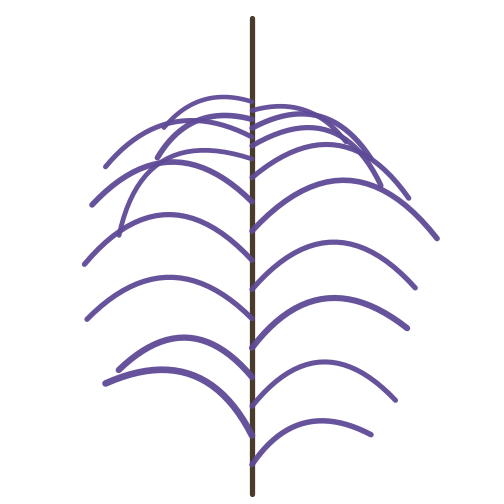
\includegraphics[width=0.8400in, height=0.8400in]{Figures/fig3/maize_text.png}};
\node[anchor=base west, inner sep=0, text=c111111, rotate=0, font={\fontsize{9.0}{10.8}\selectfont\sffamily\bfseries}] at (0.0200,1.1300) {c};
\node[anchor=base west, inner sep=0, text=c111111, rotate=0, font={\fontsize{6.2}{7.4}\selectfont\sffamily}] at (0.1800,1.1300) {Ten cameras per plant (five shown), by elevation};
\draw[draw=c809EC2, line width=1.00pt, rounded corners=2.88pt, fill=cE6ECF3] (0.2600,0.5600) rectangle (2.1800,0.9800);
\node[anchor=center, inner sep=0, text=c111111, rotate=90, font={\fontsize{5.8}{7.0}\selectfont\sffamily\bfseries}] at (0.1500,0.7700) {sorghum};
\node[anchor=south west, inner sep=0] at (0.3000,0.6000) {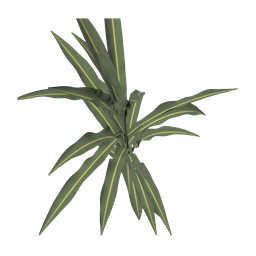
\includegraphics[width=0.3400in, height=0.3400in]{Figures/fig3/sorghum_camera_0.png}};
\node[anchor=south, inner sep=0, text=c444444, rotate=0, font={\fontsize{5.4}{6.5}\selectfont\sffamily}] at (0.4700,0.9900) {+64$^{\circ}$};
\node[anchor=south west, inner sep=0] at (0.6750,0.6000) {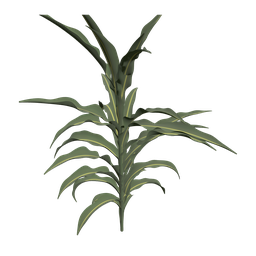
\includegraphics[width=0.3400in, height=0.3400in]{Figures/fig3/sorghum_camera_1.png}};
\node[anchor=south, inner sep=0, text=c444444, rotate=0, font={\fontsize{5.4}{6.5}\selectfont\sffamily}] at (0.8450,0.9900) {+30$^{\circ}$};
\node[anchor=south west, inner sep=0] at (1.0500,0.6000) {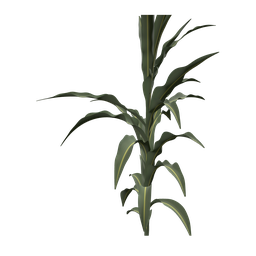
\includegraphics[width=0.3400in, height=0.3400in]{Figures/fig3/sorghum_camera_2.png}};
\node[anchor=south, inner sep=0, text=c444444, rotate=0, font={\fontsize{5.4}{6.5}\selectfont\sffamily}] at (1.2200,0.9900) {+6$^{\circ}$};
\node[anchor=south west, inner sep=0] at (1.4250,0.6000) {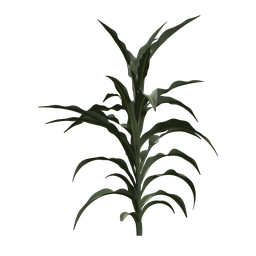
\includegraphics[width=0.3400in, height=0.3400in]{Figures/fig3/sorghum_camera_3.png}};
\node[anchor=south, inner sep=0, text=c444444, rotate=0, font={\fontsize{5.4}{6.5}\selectfont\sffamily}] at (1.5950,0.9900) {$-$17$^{\circ}$};
\node[anchor=south west, inner sep=0] at (1.8000,0.6000) {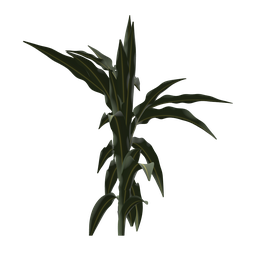
\includegraphics[width=0.3400in, height=0.3400in]{Figures/fig3/sorghum_camera_4.png}};
\node[anchor=south, inner sep=0, text=c444444, rotate=0, font={\fontsize{5.4}{6.5}\selectfont\sffamily}] at (1.9700,0.9900) {$-$44$^{\circ}$};
\draw[draw=c809EC2, line width=1.00pt, rounded corners=2.88pt, fill=cE6ECF3] (0.2600,0.0300) rectangle (2.1800,0.4500);
\node[anchor=center, inner sep=0, text=c111111, rotate=90, font={\fontsize{5.8}{7.0}\selectfont\sffamily\bfseries}] at (0.1500,0.2400) {maize};
\node[anchor=south west, inner sep=0] at (0.3000,0.0700) {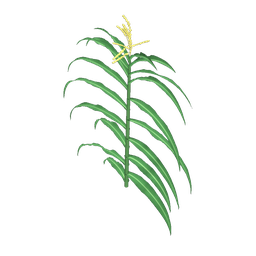
\includegraphics[width=0.3400in, height=0.3400in]{Figures/fig3/maize_camera_0.png}};
\node[anchor=south, inner sep=0, text=c444444, rotate=0, font={\fontsize{5.4}{6.5}\selectfont\sffamily}] at (0.4700,0.4600) {+39$^{\circ}$};
\node[anchor=south west, inner sep=0] at (0.6750,0.0700) {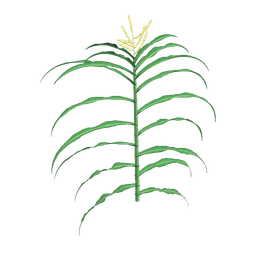
\includegraphics[width=0.3400in, height=0.3400in]{Figures/fig3/maize_camera_1.png}};
\node[anchor=south, inner sep=0, text=c444444, rotate=0, font={\fontsize{5.4}{6.5}\selectfont\sffamily}] at (0.8450,0.4600) {+30$^{\circ}$};
\node[anchor=south west, inner sep=0] at (1.0500,0.0700) {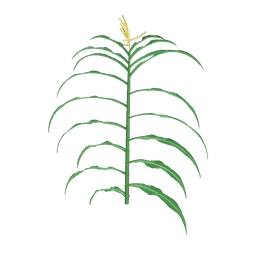
\includegraphics[width=0.3400in, height=0.3400in]{Figures/fig3/maize_camera_2.png}};
\node[anchor=south, inner sep=0, text=c444444, rotate=0, font={\fontsize{5.4}{6.5}\selectfont\sffamily}] at (1.2200,0.4600) {+10$^{\circ}$};
\node[anchor=south west, inner sep=0] at (1.4250,0.0700) {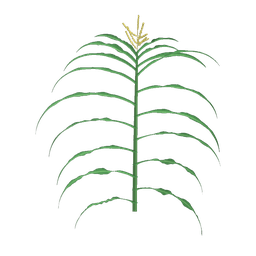
\includegraphics[width=0.3400in, height=0.3400in]{Figures/fig3/maize_camera_3.png}};
\node[anchor=south, inner sep=0, text=c444444, rotate=0, font={\fontsize{5.4}{6.5}\selectfont\sffamily}] at (1.5950,0.4600) {$-$13$^{\circ}$};
\node[anchor=south west, inner sep=0] at (1.8000,0.0700) {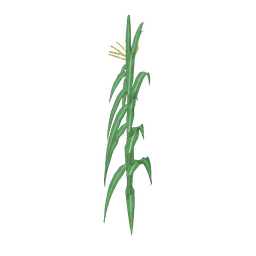
\includegraphics[width=0.3400in, height=0.3400in]{Figures/fig3/maize_camera_4.png}};
\node[anchor=south, inner sep=0, text=c444444, rotate=0, font={\fontsize{5.4}{6.5}\selectfont\sffamily}] at (1.9700,0.4600) {$-$36$^{\circ}$};
\node[anchor=base west, inner sep=0, text=c111111, rotate=0, font={\fontsize{9.0}{10.8}\selectfont\sffamily\bfseries}] at (2.8400,1.1300) {d};
\node[anchor=base west, inner sep=0, text=c111111, rotate=0, font={\fontsize{6.2}{7.4}\selectfont\sffamily}] at (3.0000,1.1300) {Crop rows: the target plant between neighbors};
\node[anchor=base west, inner sep=0, text=c555555, rotate=0, font={\fontsize{5.4}{6.5}\selectfont\sffamily}] at (3.0000,1.0250) {red: neighbor pixels;  orange: target pixels a neighbor hides (\% hidden);  green: target points};
\node[anchor=base, inner sep=0, text=c111111, rotate=0, font={\fontsize{6.2}{7.4}\selectfont\sffamily\bfseries}] at (3.7600,0.9350) {sorghum};
\draw[draw=c809EC2, line width=1.00pt, rounded corners=3.60pt, fill=cE6ECF3] (2.9900,0.1300) rectangle (3.7500,0.8900);
\node[anchor=south west, inner sep=0] at (3.0200,0.1600) {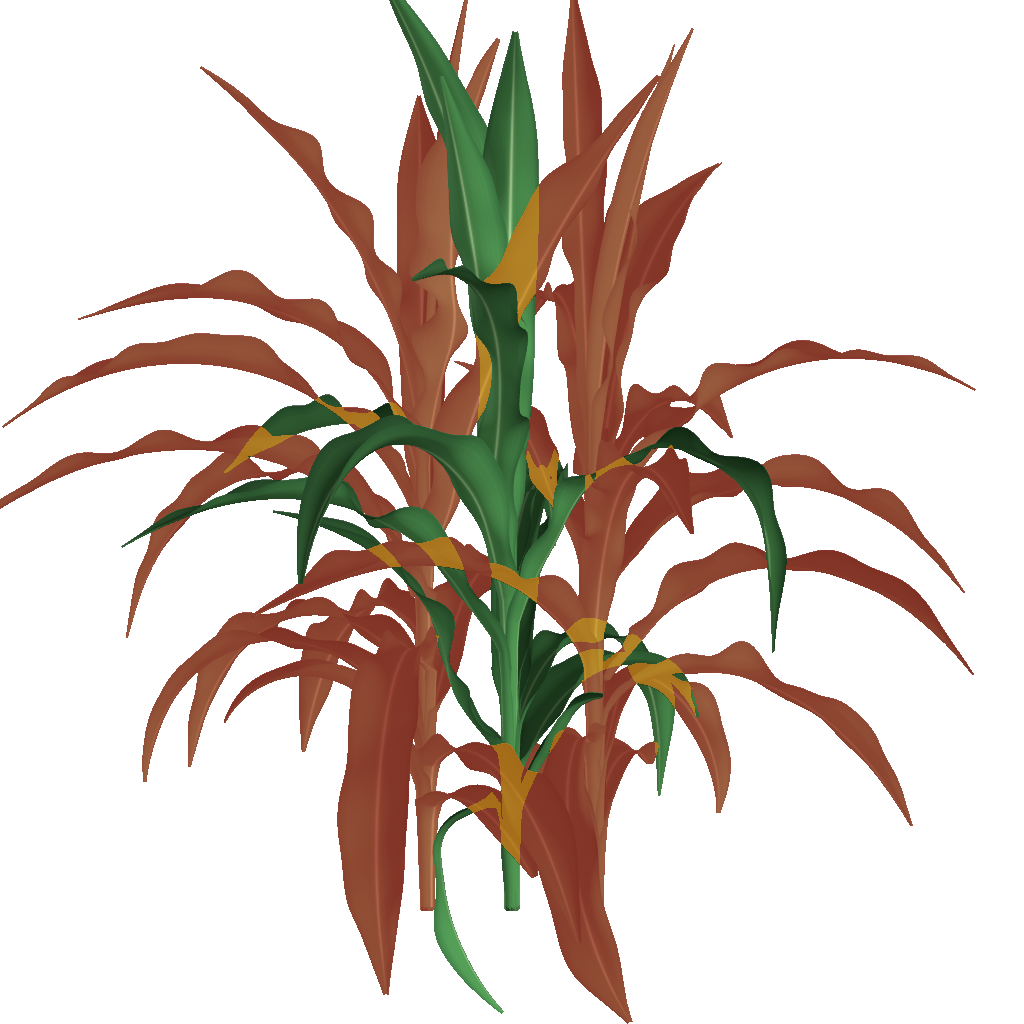
\includegraphics[width=0.7000in, height=0.7000in]{Figures/fig3/sorghum_row_image.png}};
\node[anchor=north, inner sep=0, text=c111111, rotate=0, font={\fontsize{5.6}{6.7}\selectfont\sffamily}] at (3.3700,0.1000) {16 \% hidden};
\draw[draw=cD091A7, line width=1.00pt, rounded corners=3.60pt, fill=cF6E9ED] (3.7700,0.1300) rectangle (4.5300,0.8900);
\node[anchor=south west, inner sep=0] at (3.8000,0.1600) {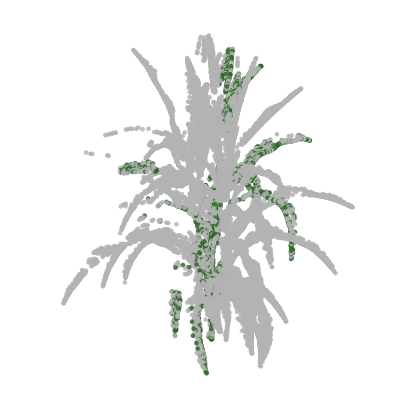
\includegraphics[width=0.7000in, height=0.7000in]{Figures/fig3/sorghum_row_cloud.png}};
\node[anchor=north, inner sep=0, text=c111111, rotate=0, font={\fontsize{5.6}{6.7}\selectfont\sffamily}] at (4.1500,0.1000) {89 \% neighbors};
\node[anchor=base, inner sep=0, text=c111111, rotate=0, font={\fontsize{6.2}{7.4}\selectfont\sffamily\bfseries}] at (5.5400,0.9350) {maize};
\draw[draw=c809EC2, line width=1.00pt, rounded corners=3.60pt, fill=cE6ECF3] (4.7700,0.1300) rectangle (5.5300,0.8900);
\node[anchor=south west, inner sep=0] at (4.8000,0.1600) {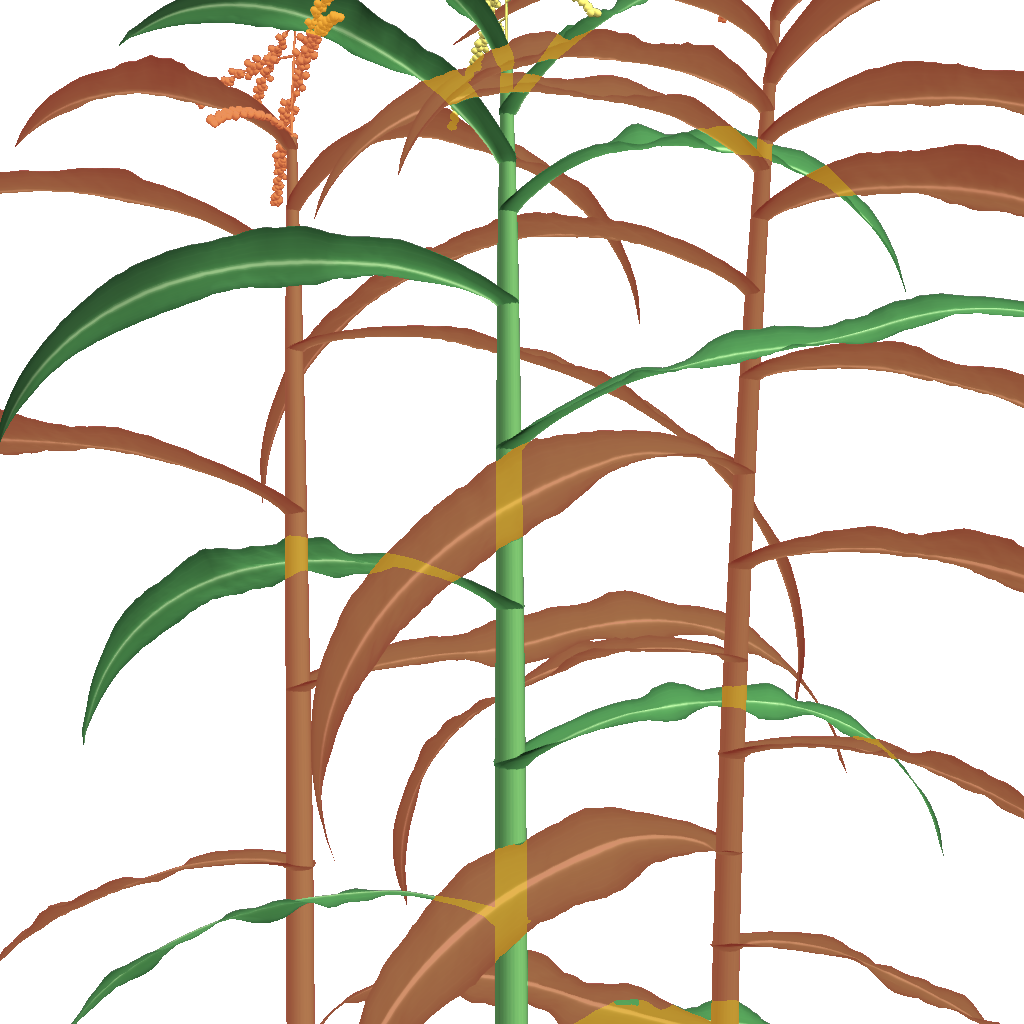
\includegraphics[width=0.7000in, height=0.7000in]{Figures/fig3/maize_row_image.png}};
\node[anchor=north, inner sep=0, text=c111111, rotate=0, font={\fontsize{5.6}{6.7}\selectfont\sffamily}] at (5.1500,0.1000) {15 \% hidden};
\draw[draw=cD091A7, line width=1.00pt, rounded corners=3.60pt, fill=cF6E9ED] (5.5500,0.1300) rectangle (6.3100,0.8900);
\node[anchor=south west, inner sep=0] at (5.5800,0.1600) {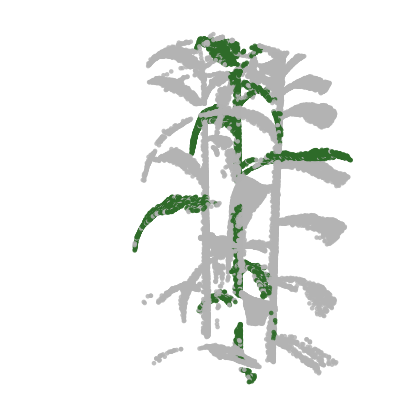
\includegraphics[width=0.7000in, height=0.7000in]{Figures/fig3/maize_row_cloud.png}};
\node[anchor=north, inner sep=0, text=c111111, rotate=0, font={\fontsize{5.6}{6.7}\selectfont\sffamily}] at (5.9300,0.1000) {75 \% neighbors};
\end{tikzpicture}
}
  \caption{\textbf{\dataset{} at a glance.} (a) Six of the 15{,}000 plants of each species (validation split, side view). (b) One view of the boxed plant as its four streams: image, depth image, camera-frame point cloud and the procedural parameters, drawn as a stem with each leaf at its insertion height, length, width and side. (c) Five of the ten cameras of that plant, labelled by elevation above the plant: sorghum on a fixed ladder from $+64^\circ$ to $-64^\circ$, maize at random elevations and azimuths (sorted here). (d) One row scene per species at yaw $0^\circ$: the row image with neighbor pixels in red and target pixels hidden behind a neighbor in orange, and the scene point cloud with the target plant's points in green and the neighbors' points in grey.}
  \label{fig:dataset}
\end{figure*}

\begin{figure*}[t]
  \centering
  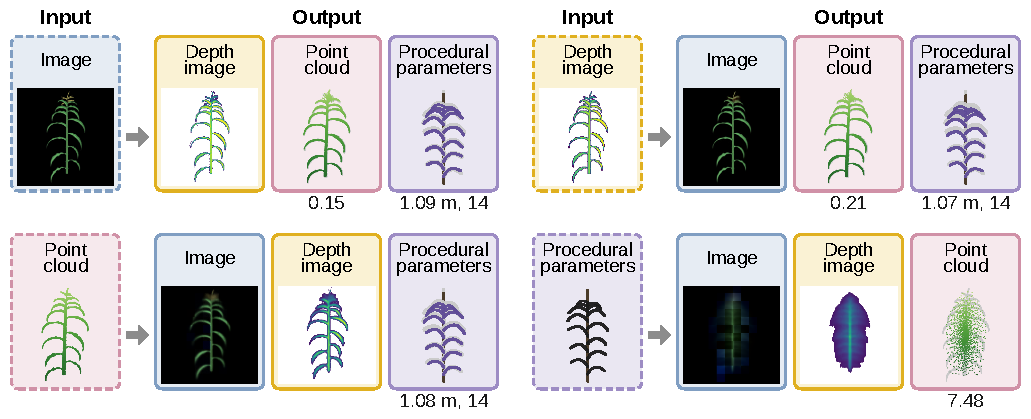
\includegraphics[width=\linewidth]{Figures/fig_any2all_maize_ugg.pdf}
  \caption{\textbf{Any-to-all, maize: each stream alone in, the other three out.} The distilled generalist on one held-out test plant. Each block gives it one stream (dashed box, left of the grey arrow) and shows the three streams it generates (solid boxes); the box color marks the stream: image blue, depth yellow, point cloud pink, procedural parameters purple. Generated point clouds and procedural parameters are drawn over the ground truth in grey, the parameters as a stem-and-leaves schematic. Under each generated point cloud: its Chamfer distance ($10^{-3}$); under each generated parameter set: height and leaf count (truth 1.12\,m, 14 leaves). The plant is selected for clarity among the test plants with the lowest image-to-cloud Chamfer, seen within $25^\circ$ of the horizon. The parameters alone give only a coarse plant (Chamfer 7.48 here, 12.8 on average in Table~\ref{tab:anysubset}).}
  \label{fig:any2any-maize}\label{fig:any2any}
\end{figure*}

\begin{figure*}[t]
  \centering
  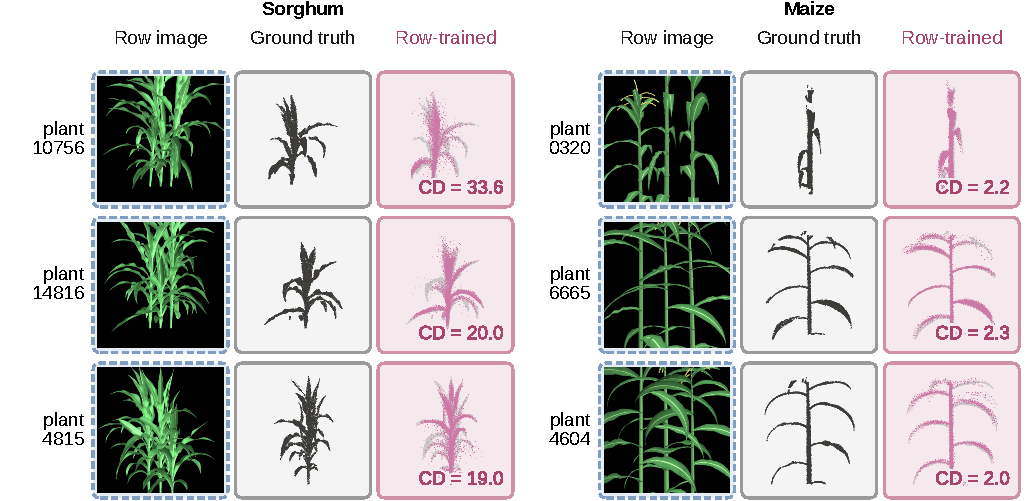
\includegraphics[width=\linewidth]{Figures/fig_rows_examples_ugg.pdf}
  \caption{\textbf{Row occlusion reconstruction on held-out test plants.} Sorghum (left) and maize (right). Columns: the row image the model reads (neighbors included), the center plant's ground-truth point cloud, and the point cloud written by the row-trained model (pink) over the ground truth in grey; CD is its Chamfer distance to the ground truth in $10^{-4}\,\mathrm{m}^2$ (lower is better). The plants were selected for clarity among those where the row-trained model is in its best 35\% and the isolated-trained control in its worst 40\% at both yaws (broadside and end-on); Figs.~\ref{fig:supp-rows-sorghum} and~\ref{fig:supp-rows-maize} show ten more plants per species, spread over the whole error range.}
  \label{fig:rowsex}
\end{figure*}

\begin{table}[t]
  \caption{\textbf{\dataset{} dataset configuration.} Parameter dimensions
  include macro plant-level traits plus $K$ structured leaf parameter
  slots. Every row scene pairs a target main plant with two adjacent row
  neighbors spaced at 0.15\,m stem intervals.}
  \label{tab:fieldproc}
  \centering\scriptsize
  \setlength{\tabcolsep}{3pt}
  \begin{tabular}{lcc}
    \toprule
    Parameter / Configuration & Maize & Sorghum \\
    \midrule
    Total generated plants & 15{,}000 & 15{,}000 \\
    Split (train / val / test) & \multicolumn{2}{c}{10{,}500 / 2{,}250 / 2{,}250} \\
    Views per plant & 10 (random sphere) & 10 (fixed rig) \\
    Camera distance & box-fitted & 2.5\,m \\
    Per-view point cloud & 8{,}192 pts (visible) & complete plant cloud \\
    Parameter dim.\ $d_\theta$ & $14{+}14{\times}28{=}406$ & $9{+}5{\times}24{=}129$ \\
    Leaf count range & 3--22 & 4--35 \\
    Plant height range & 0.62--1.44\,m & 0.19--1.74\,m (stem) \\
    Row scenes $\times$ orientations & $15{,}000 \times 10$ & $15{,}000 \times 10$ \\
    Row camera & level rover, 1.0\,m & level rover, 2.5\,m \\
    Row cloud (input / target) & \multicolumn{2}{c}{24{,}576 / 8{,}192 pts} \\
    Real-field split & 520 real plants, 2 layouts & 30 scanned plants, 2 layouts \\
    \bottomrule
  \end{tabular}
  
\end{table}

\noindent\textbf{Generation in brief.}
Each species' generator draws 15{,}000 plants: maize 0.62--1.44\,m
tall with 3--22 leaves, its traits coupled through four latent factors so
that height and leaf count stay weakly correlated ($r = 0.20$); sorghum
(EvoEngine) with stems of 0.19--1.74\,m and 4--35 leaves, stem length tied
to leaf count ($R^2 = 0.988$), so the two species cover a weakly and a
strongly coupled morphological regime. Ten views per plant are rendered at
$1024^2$ ($40^\circ$ field of view) with photograph, losslessly packed
metric depth and camera calibration: sorghum from a fixed Fibonacci rig at
2.5\,m with the complete plant cloud per view, maize from random directions
at a box-fitted distance with partial 8{,}192-point clouds back-projected
from depth. Row scenes place each target between two neighbors at 0.15\,m
spacing across ten yaws ($0^\circ$--$90^\circ$, $\pm 15^\circ$ neighbor
offsets); an articulated contact solver bends leaf blades (8\,cm jointed
segments, exact triangle--triangle tests) so that neighbors yield first and
the target keeps its grown shape wherever a neighbor can give way, and a
rover camera captures the scene (RGB, depth, 24{,}576-point cloud) with the
bent target alone (8{,}192 points) as ground truth. Neighbors account for
59--68\% of plant pixels in maize rows and hide 23\% of the target's pixels
in sorghum. Plants split 70/15/15 by plant, with validation and test
enriched toward extreme morphologies by Mahalanobis ranking.
Appendix~\ref{app:data} gives the generators, the renderer, the contact
solver and the partitioning in full.

\begin{table}[t]
  \caption{\textbf{Dataset comparison.} Exact Procedural GT indicates exact
ground-truth generative parameter vectors per plant; (\cmark) denotes
parameters fitted post hoc via optimization. $^{\dagger}$\dataset{}
includes real-field evaluation scans; training splits consist of procedural
synthetic data.}
\label{tab:datacompare}
\centering\scriptsize
\setlength{\tabcolsep}{2.5pt}
\resizebox{\columnwidth}{!}{%
\begin{tabular}{lcccccc}
\toprule
Dataset & Real scans & Slender & Row occl. & RGB+D+PC & Exact proc.\ GT & Scale \\
\midrule
PCN / ShapeNet-55~\citep{yuan2018pcn,yu2021pointr} & \xmark & \xmark & \xmark & \xmark & \xmark & 55{,}000 \\
Pheno4D~\citep{schunck2021pheno4d} & \cmark & \cmark & \xmark & \xmark & \xmark & 84 \\
Crops3D~\citep{crops3d2024} & \cmark & \cmark & \xmark & \xmark & \xmark & 2{,}500 \\
MaizeField3D~\citep{maizefield3d2025} & \cmark & \cmark & \xmark & \xmark & (\cmark) & 1{,}000 \\
\textbf{\dataset{} (ours)} & \textbf{\cmark}$^{\dagger}$ & \textbf{\cmark} & \textbf{\cmark} & \textbf{\cmark} & \textbf{\cmark} & \textbf{30{,}000} \\
\bottomrule
\end{tabular}}

\end{table}

\subsection{Four-stream masked pretraining}
\label{sec:method-pretrain}

\noindent\textbf{Multimodal tokenization.}
Building on EmbodiedMAE~\cite{dong2025embodiedmae}, RGB and depth
are split into 196 patches on a $14 \times 14$ grid and linearly projected
to 768-d tokens with 2D sine--cosine positions; point clouds become 196
farthest-point-sampled groups of 32 neighbors with PointNet
features~\cite{pang2022pointmae,qi2017pointnet}; and the parameter vector
$\theta$ becomes $1 + K$ continuous numerical tokens (one plant token plus
$K$ leaf slots, $K = 28$ for maize and 24 for sorghum), affinely normalized
to $[0,1]$ and embedded xVal-style~\cite{golkar2023xval}. Learned modality
embeddings and a \texttt{[CLS]} token complete the sequence for a 12-block
ViT encoder (width 768) and an 8-block decoder (width 512), with linear
RGB and depth heads, a FoldingNet cloud head (41 points per token) and an
MLP for the parameters. Scored against ground truth, real leaf slots are
selected by the validity mask; used without ground truth
(Tab.~\ref{tab:regime1}, Appendix~\ref{app:tables}), the leaf count is read
from the recipe itself, which maize stores in the plant token and sorghum
implies through the generator's stem-length rule.

\noindent\textbf{Dynamic Dirichlet masking.}
A total masking budget of $\rho = 0.80$ leaves
$V = \lfloor (1-\rho)L \rfloor$ visible tokens (122 of $L = 613$ for
sorghum, 123 of 617 for maize), allocated across streams by a symmetric
Dirichlet draw at every step, each stream keeping at least one visible and
25\% masked tokens, so one network learns to complete any modality subset.
The parameter stream sits inside this shared budget in the headline setup
($\sim$58\% visible on average); the control arms of
Sec.~\ref{sec:exp-params} instead gate it at a fixed visibility
$\rho_\theta$, with $\rho_\theta = 1$ making the parameters a decoder-only
reconstruction target.

\noindent\textbf{Multi-term reconstruction objective.}
The objective sums modality losses,
\begin{equation}
  \mathcal{L}_{\mathrm{rec}} = \ell_{\mathrm{rgb}} + \ell_{\mathrm{d}} + \ell_{\mathrm{pc}} + 5\ell_\theta.
  \label{eq:reconstruction-loss}
\end{equation}
with $\ell_{\mathrm{rgb}}$ MSE on patch-normalized
pixels~\cite{he2022mae}, $\ell_{\mathrm{d}}$ MSE on min--max normalized
depth, and $\ell_\theta$ Smooth-$L_1$ on masked parameter tokens. Standard
Chamfer lets many predicted points match one target point, collapsing
decoders onto stems~\cite{wu2021dcd,song2026structural}, so the cloud loss
is sigmoid-weighted,
\begin{equation}
  \ell_{\mathrm{pc}} = \frac{1}{|\hat P|}\sum_{p\in\hat P}w(\delta(p,P))\,\delta(p,P) + \frac{1}{|P|}\sum_{q\in P}w(\delta(q,\hat P))\,\delta(q,\hat P),
 \label{eq:point-loss}
\end{equation}
with $\delta(p,P) = \min_{q \in P} \|p - q\|_2$,
$w(r) = \sigma(a(r - \tau))$, $a = 100$ and $\tau = 0.01$ of the unit
sphere, and the headline setup adds a debiased Sinkhorn
divergence~\cite{feydy2019sinkhorn} that matches the clouds as
distributions and so penalizes missing blades,
\begin{equation}
  \ell_{\mathrm{pc}}^{\star} = \ell_{\mathrm{pc}} + 0.5\,S_{\varepsilon}\!\left(\hat P_{1024}, P_{1024}\right),
  \label{eq:point-loss-sinkhorn}
\end{equation}
on random 1{,}024-point subsets ($\varepsilon = 0.02$). Models
train with AdamW (cosine decay): the headline schedule peaks at
$6 \times 10^{-4}$ over 1{,}000 epochs of all ten views at global batch
256; ablation arms share a matched budget of 197{,}400 steps at global
batch 32, one view per plant per epoch, peaking at $1.5 \times 10^{-4}$,
with Eq.~\eqref{eq:point-loss} alone as the cloud loss.

\subsection{Full-modality teacher to single-sensor students}
\label{sec:distill}\label{sec:method-distill}

Single-sensor deployment shows the encoder a configuration
pretraining never does: every token of the unobserved streams absent. A
frozen four-stream teacher closes the gap, with the parameters as
privileged input (every token visible for sorghum; half of each stream for
maize, whose cloud reconstruction degrades when fully visible). It emits a
global latent $c^T \in \R^{768}$ and normalized decoder features
$F^T \in \R^{L \times 512}$; students start from the teacher's weights,
train 100 epochs (AdamW, $10^{-4}$, global batch 128), receive a single
source $s \in \{\mathrm{rgb}, \mathrm{d}, \mathrm{pc}, \theta\}$ on 80\% of
steps and standard four-stream pretraining on the rest, and minimize
\begin{equation}
  \mathcal{L}_{\mathrm{student}} = \mathcal{L}_{\mathrm{rec}} + \frac{\lambda_F}{|\mathcal{J}_{\neg s}|} \sum_{j \in \mathcal{J}_{\neg s}} \|F^S_j - F^T_j\|_2^2 + \lambda_c \|c^S - c^T\|_2^2,
  \label{eq:distillation-loss}
\end{equation}
where $\mathcal{J}_{\neg s}$ are the decoder positions of the
unobserved non-source streams ($\lambda_F = 1.0$, $\lambda_c = 0.5$). At
deployment each sensor is evaluated alone.

\noindent\textbf{Field evaluation and transfer protocols.}

We evaluate in three regimes. \textbf{(1) Trait probing}: ridge
probes on frozen \texttt{[CLS]} tokens, fit on the training plants and
scored on the held-out splits with one deterministic view per plant and the
parameter inputs zeroed against label leakage; a change counts as a win
only when its 95\% paired-bootstrap interval (2{,}000 resamples over
plants) excludes zero on validation and test. Under partial clouds the
probe is refit per visibility condition (\emph{matched}) or applied
unchanged from the complete-cloud fit (\emph{transferred}).
\textbf{(2) Rows}: zero-shot transfer of isolated-trained models, and row
fine-tuning that reconstructs the target plant behind its neighbors, with
an isolated-control arm on the same schedule and an echo test that scores
generated clouds against both the target and the input scene.
\textbf{(3) Real-field validation} on MaizeField3D
captures~\citep{maizefield3d2025}, against the procedural fits of a staged
vision-language pipeline~\citep{hadadi2026vlmmaize} as independently
reconstructed ground truth.

\section{Experiments}
\label{sec:results}\label{sec:experiments}
Unless a figure number five or lower is named, the figures referenced in this and the following sections are in Appendix~\ref{app:figures}.

In this section, we present an extensive experimental evaluation of
\method{}. We describe our experimental setup (Sec.~\ref{sec:exp-setup}),
followed by evaluations across three deployment regimes: isolated
single-view reconstruction (Sec.~\ref{sec:exp-regime1}), difficulty
progression across viewpoint and self-occlusion (Sec.~\ref{sec:exp-regime2}),
and neighbor occlusion in realistic field rows
(Sec.~\ref{sec:exp-occlusion}). We then analyze cross-modal distillation
(Sec.~\ref{sec:exp-main}), investigate the placement of the procedural
parameter stream (Sec.~\ref{sec:exp-params}), uncover systematic
divergences between geometric metrics and downstream trait probes
(Sec.~\ref{sec:exp-metrics}), describe the real-field validation protocol
(Sec.~\ref{sec:exp-real}), and analyze scaling, cross-species transfer, and
latent space structure (Sec.~\ref{sec:exp-repr}).

\noindent\textbf{Experimental setup.}
\label{sec:setup}\label{sec:exp-setup}

\noindent\textbf{Models and compute budgets.}
All ablation arms share 197{,}400 optimizer steps at global batch 32
(600 epochs of one random view per plant), identical view-sampling seeds and
a ViT-Base encoder (114\,M parameters) unless capacity is varied;
data-scale arms adjust their epoch counts to keep the step budget. The
headline model trains for 1{,}000 epochs on all ten views at global batch
256 with the Sinkhorn term and initializes every teacher and student of
Sec.~\ref{sec:exp-main}. Results are on the validation split unless stated
otherwise.

\noindent\textbf{Evaluation metrics.} Chamfer is the symmetric squared
distance in the unit-sphere frame ($\times 10^{-3}$), trait \emph{skill} is
1 for perfect recovery and 0 for predicting the dataset mean, and
representation quality is the frozen-probe $R^2$ with the paired-bootstrap
win criterion of Sec.~\ref{sec:method}; Appendix~\ref{app:metrics} gives
the full definitions, the per-plant millimetre conversion and each
species' trait set.

\begin{table*}[t]
  \caption{\textbf{Comparison against published pre-trained encoders (E8).}
  Published self-supervised visual encoders are evaluated on identical
  held-out validation plants using mean-pooled features and the same ridge
  regression probe protocol. Every row is mean-pooled, including the
  headline model of each species at epoch 1{,}000. Values are validation $R^2$ (higher is better); bold marks the best value in each column.}
  \label{tab:e8}\label{tab:baselines}
  \centering\scriptsize
  \setlength{\tabcolsep}{2.6pt}
  \begin{tabular}{l ccc cc c cccc}
    \toprule
    & \multicolumn{5}{c}{Sorghum} & & \multicolumn{4}{c}{Maize} \\
    \cmidrule(lr){2-6}\cmidrule(lr){8-11}
    Frozen Encoder & Height & Leaf Cnt & Branch & Roll & Leaf Len & & Height & Leaf Angle & Curl & Stem Rad \\
    \midrule
    DINOv2 ViT-B/14 (RGB)~\cite{oquab2024dinov2} & 0.924 & 0.928 & 0.840 & 0.573 & 0.235 & & 0.561 & 0.816 & 0.072 & 0.588 \\
    MultiMAE-B (RGB+D)~\cite{bachmann2022multimae} & 0.922 & 0.925 & 0.833 & 0.679 & 0.232 & & 0.570 & 0.783 & 0.069 & 0.442 \\
    Point-MAE (PC)~\cite{pang2022pointmae} & 0.958 & 0.963 & 0.863 & 0.716 & 0.188 & & 0.509 & 0.863 & 0.199 & 0.426 \\
    EmbodiedMAE-B (RGB+D+PC)~\cite{dong2025embodiedmae} & 0.976 & 0.979 & 0.871 & 0.765 & 0.265 & & 0.528 & 0.823 & 0.139 & 0.428 \\
    \CropCode{} Headline (1{,}000 ep) & \textbf{0.983} & \textbf{0.988} & \textbf{0.912} & \textbf{0.798} & \textbf{0.371} & & \textbf{0.747} & \textbf{0.967} & \textbf{0.739} & \textbf{0.841} \\
    \bottomrule
  \end{tabular}
  
\end{table*}

\begin{table*}[t]
  \caption{\textbf{Ablations at the shared step budget (197{,}400 optimizer steps).} \textbf{(a)}~Modality value-add: models differing only in active input token streams; $\theta$ is the parameter stream as an encoder input under the shared Dirichlet budget. \textbf{(b)}~Dataset scale and encoder capacity: at fixed step compute, larger encoders do not help and more data helps reconstruction more reliably than it helps the probes. Chamfer $\times 10^{-3}$ and linear-probe $R^2$ (validation).}
  \label{tab:e2}\label{tab:modality_value_add}\label{tab:scaling}\label{tab:scaling_ablations}
  \centering\scriptsize
  \begin{minipage}[t]{0.52\textwidth}
    \centering
    \textbf{(a) Modality value-add}\\[3pt]
    \setlength{\tabcolsep}{3.2pt}
    \resizebox{\linewidth}{!}{%
    \begin{tabular}{l c cccccc}
    \toprule
    & Chamfer & \multicolumn{6}{c}{Frozen-Probe $R^2$ (Validation Set)} \\
    \cmidrule(lr){3-8}
    Stream Set & $\times10^{-3}$ & Height & Leaf Cnt & Biomass & Branch & Roll & Leaf Len \\
    \midrule
    \multicolumn{8}{l}{\emph{Sorghum}} \\
    PC & 5.00 & 0.895 & 0.896 & 0.892 & 0.792 & 0.393 & 0.088 \\
    $\mathrm{PC}+\mathrm{D}$ & 2.45 & 0.976 & 0.979 & 0.982 & 0.903 & 0.798 & 0.307 \\
    $\mathrm{PC}+\mathrm{RGB}$ & 2.57 & \textbf{0.979} & \textbf{0.983} & \textbf{0.986} & \textbf{0.934} & 0.808 & 0.267 \\
    $\mathrm{PC}+\mathrm{RGB}+\mathrm{D}$ & \textbf{1.85} & 0.977 & 0.980 & 0.982 & 0.926 & 0.781 & \textbf{0.309} \\
    $\mathrm{PC}+\theta$ & 4.84 & 0.860 & 0.864 & 0.863 & 0.780 & 0.481 & 0.078 \\
    $\mathrm{PC}+\mathrm{D}+\theta$ & 4.08 & 0.907 & 0.909 & 0.916 & 0.856 & 0.694 & 0.191 \\
    $\mathrm{PC}+\mathrm{RGB}+\theta$ & 3.00 & 0.962 & 0.964 & 0.967 & 0.890 & \textbf{0.810} & 0.225 \\
    $\mathrm{PC}+\mathrm{RGB}+\mathrm{D}+\theta$ & 2.53 & 0.962 & 0.964 & 0.965 & 0.880 & 0.760 & 0.249 \\
    \midrule
    & & Height & Leaf Cnt & Biomass & Branch & Curl & Stem Rad \\
    \multicolumn{8}{l}{\emph{Maize}} \\
    PC & 2.63 & 0.171 & 0.670 & 0.610 & 0.756 & 0.114 & 0.289 \\
    $\mathrm{PC}+\mathrm{D}$ & 2.55 & 0.453 & 0.773 & 0.683 & 0.804 & 0.082 & 0.550 \\
    $\mathrm{PC}+\mathrm{RGB}$ & 1.61 & 0.620 & \textbf{0.914} & \textbf{0.783} & \textbf{0.927} & 0.334 & 0.753 \\
    $\mathrm{PC}+\mathrm{RGB}+\mathrm{D}$ & 1.21 & 0.633 & \textbf{0.914} & 0.774 & 0.926 & 0.236 & 0.760 \\
    $\mathrm{PC}+\theta$ & 2.49 & 0.256 & 0.740 & 0.662 & 0.787 & 0.114 & 0.363 \\
    $\mathrm{PC}+\mathrm{D}+\theta$ & 2.54 & 0.382 & 0.801 & 0.670 & 0.795 & 0.136 & 0.408 \\
    $\mathrm{PC}+\mathrm{RGB}+\theta$ & 1.21 & 0.509 & 0.881 & 0.780 & 0.912 & \textbf{0.371} & \textbf{0.763} \\
    $\mathrm{PC}+\mathrm{RGB}+\mathrm{D}+\theta$ & \textbf{0.99} & \textbf{0.635} & 0.908 & 0.781 & 0.919 & 0.304 & 0.743 \\
    \bottomrule
  \end{tabular}}
  \end{minipage}\hfill
  \begin{minipage}[t]{0.45\textwidth}
    \centering
    \textbf{(b) Training dataset scale and encoder capacity}\\[3pt]
    \setlength{\tabcolsep}{3.0pt}
    \resizebox{\linewidth}{!}{%
    \begin{tabular}{l r c ccc}
    \toprule
    Dataset / Capacity Variant & Epochs & Chamfer & Height & Roll & Leaf Len \\
    \midrule
    \multicolumn{6}{l}{\emph{Sorghum: Training Dataset Scale (Base Model)}} \\
    1{,}000 Plants & 6{,}169 & 3.13 & 0.952 & 0.716 & 0.249 \\
    3{,}000 Plants & 2{,}100 & 2.86 & 0.932 & 0.679 & 0.213 \\
    10{,}000 Plants & 631 & 2.48 & 0.962 & 0.749 & 0.245 \\
    10{,}500 Plants & 600 & 2.53 & 0.962 & 0.760 & 0.249 \\
    \multicolumn{6}{l}{\emph{Sorghum: Encoder Capacity (Full Dataset)}} \\
    ViT-Small (25\,M) & 600 & 2.86 & 0.964 & \textbf{0.817} & \textbf{0.277} \\
    ViT-Base (114\,M) & 600 & \textbf{2.53} & 0.962 & 0.760 & 0.249 \\
    ViT-Large (332\,M) & 600 & 2.68 & 0.948 & 0.711 & 0.246 \\
    \midrule
    & & Chamfer & Height & Branch & Stem Rad \\
    \multicolumn{6}{l}{\emph{Maize: Training Dataset Scale (Base Model)}} \\
    1{,}000 Plants & 6{,}169 & 3.54 & 0.393 & 0.851 & 0.593 \\
    3{,}000 Plants & 2{,}100 & 1.46 & 0.524 & 0.867 & 0.624 \\
    10{,}000 Plants & 631 & 0.87 & 0.427 & 0.853 & 0.717 \\
    10{,}500 Plants & 600 & 0.99 & 0.635 & 0.919 & 0.743 \\
    \multicolumn{6}{l}{\emph{Maize: Encoder Capacity (Full Dataset)}} \\
    ViT-Small (25\,M) & 600 & 1.22 & 0.563 & 0.886 & 0.682 \\
    ViT-Base (114\,M) & 600 & \textbf{0.99} & \textbf{0.635} & \textbf{0.919} & \textbf{0.743} \\
    ViT-Large (332\,M) & 600 & 1.06 & 0.580 & 0.887 & 0.614 \\
    \bottomrule
  \end{tabular}}
  \end{minipage}
  
\end{table*}

\noindent\textbf{Regime I: single-view reconstruction of isolated plants.}
\label{sec:regime1}\label{sec:exp-regime1}

Table~\ref{tab:regime1} (Appendix~\ref{app:tables}) covers
deployment on an isolated plant: one photograph, one depth frame or one
point cloud in, the recipe and the other streams out in a single forward
pass. Depth is the best single input for the cloud in both species (Chamfer
$0.93$ in sorghum and $0.64 \times 10^{-3}$ in maize, a median of $30$ and
$12$\,mm RMS per plant, $F_1$ $0.44$ and $0.53$), with the photograph
within a factor of 1.5 of it; on the full test split, photograph-to-cloud
Chamfer corresponds to a skill of $0.98$--$0.99$ against the distance
between two random plants (Sec.~\ref{sec:res-distill}). The recipe is
recovered from any single sensor: leaf count within one leaf for
$91$--$100\%$ of plants, height within $2$--$5\%$, and mean leaf-parameter
skill $0.66$--$0.68$ in sorghum and $0.57$--$0.59$ in maize, high on the
leaf's stem position and angle, moderate on length, and lowest on sorghum
blade width, whose between-plant spread is small. The headline model given
all three streams is no better than the generalist given one, because it
was never trained to read every token of its input; the first release's
three unrecoverable waviness fields are absent from the final generator.
Averaging the recipes of three views improves every recipe column, while
reading the recipe from a generated cloud loses almost all of it, so the
recipe is read from the sensor directly (Tab.~\ref{tab:regime1}).
Figure~\ref{fig:qual} (Appendix~\ref{app:figures}) shows single-photograph
reconstructions: the distilled generalist resolves individual leaf blades
where the undistilled model generates diffuse clouds, and the procedural
output can be edited and re-rendered.

\noindent\textbf{Regime II: viewpoint elevation, self-occlusion, and complexity.}
\label{sec:regime2}\label{sec:exp-regime2}

\noindent\textbf{Viewpoint elevation.}
Every view of a plant shares the same ground truth, so the elevation
ladder isolates the sensor input. Photograph-to-cloud error follows a
symmetric U over camera elevation, lowest side-on and highest looking
steeply down or up; elevation explains $\eta^2 = 0.24$--$0.31$ of per-plant
error variance while morphology correlates negligibly ($|\rho| \le 0.06$),
and distillation cuts the error by 28\% across views without flattening the
curve (Fig.~\ref{fig:views}A).

\noindent\textbf{Training view distribution.}
Pretraining restricted to elevation bands (top-down
$i \in \{0,1\}$, horizontal $i \in \{4,5\}$, or the single view 0) wins only
on the trained elevations and loses elsewhere: the sorghum per-view probe
drops by $0.066$--$0.144$ on distant views while the all-view arm holds
$R^2 = 0.734$--$0.778$ (Fig.~\ref{fig:e5views}), and in maize, probed at a
random camera, every restricted arm loses 10--11 of 11 targets under paired
bootstraps, with the point-cloud $F_1$ agreeing. Covering the evaluation
elevations matters more than the number of images;
Appendix~\ref{app:views-full} gives the per-arm numbers.

\noindent\textbf{Self-occlusion under partial camera coverage.}
Clipping point clouds by mesh ray-casting to the surface visible
from 1 or 3 cameras (49\% and 78\% coverage) leaves trait information intact
when the probe is refit (height $R^2$ 0.960 at one camera for the headline
model) but breaks a probe transferred from complete clouds
($R^2 \to -0.26$; Fig.~\ref{fig:partial}, Tab.~\ref{tab:views},
Appendix~\ref{app:tables}). Partial visibility is a covariate shift in the
latent space: field readouts must be refit on sensor-matched coverage.

\noindent\textbf{Morphological complexity.}
After distillation, reconstruction error is flat across leaf-count
deciles (Spearman $\rho = -0.07$ in sorghum, $+0.04$ in maize;
Fig.~\ref{fig:leafcount}).

\noindent\textbf{Regime III: neighbor occlusion in realistic crop rows.}
\label{sec:regime3}\label{sec:exp-occlusion}

Table~\ref{tab:regime_3} (Appendix~\ref{app:tables}) compares
identical plants in isolation and inside rows. Models trained on isolated
plants fail under row occlusion, with Chamfer rising sixteenfold on maize
($1.8 \to 29.0 \times 10^{-4}\,\mathrm{m}^2$) and tenfold on sorghum
($13.1 \to 133.8$); the echo test shows they reconstruct neighboring foliage
as the target. Row fine-tuning removes 92\% of the neighbor-induced error in
maize ($29.0 \to 4.0$) and 85\% in sorghum ($133.8 \to 30.7$), isolating the
target behind its neighbors (Fig.~\ref{fig:rowsex}). Error peaks broadside
and falls end-on in maize, whose leaf planes align with the row, and is
yaw-independent in sorghum, whose headings are random
(Fig.~\ref{fig:row_reconstruction_quant}, Appendix~\ref{app:figures}).

\noindent\textbf{Any-subset modality reconstruction and distillation.}
\label{sec:res-distill}\label{sec:exp-main}

Table~\ref{tab:main} (Appendix~\ref{app:tables}) reports
cross-modal generation before and after distillation, and
Figs.~\ref{fig:any2any-maize} and~\ref{fig:any2any-sorghum} show the
generalist's outputs. Distillation cuts the mean generation loss by 30.2\%
in sorghum and 43.5\% in maize: photograph-to-cloud Chamfer falls 61\%
($2.27 \to 0.88 \times 10^{-3}$), photograph parameter MAE 76\%
($0.058 \to 0.014$), and point-cloud parameter MAE halves
($0.040 \to 0.020$). Sensor-plus-recipe pairs reach the lowest cloud errors
($0.36$--$0.44 \times 10^{-3}$), and one student trained on all three input
pairs matches the dedicated two-stream students within $0.03$ in both
species.

\noindent\textbf{Influence of procedural parameter stream placement.}
\label{sec:param-stream}\label{sec:exp-params}

Tables~\ref{tab:modality_value_add} and~\ref{tab:token_budget}
(Appendix~\ref{app:tables}) vary the active streams and the parameter
stream's visibility. The image streams carry the trait information: adding
RGB or depth to point clouds lifts sorghum height $R^2$ from $0.895$ to
$0.979$ and $0.976$, and RGB lifts maize from $0.171$ to $0.620$, while
depth's 25--28\% Chamfer gain leaves the probes nearly unchanged. Parameter
tokens visible to the encoder state the targets outright, and the
budget-matched controls separate the mechanisms: with the sensor-token
budget restored, sorghum still loses on every target at any parameter
visibility, including target-only supervision ($0.966$ against $0.977$ on
height), whereas maize improves on all eleven traits with the parameters
gated to 20\% or used only as a reconstruction target ($0.776$ against
$0.633$ on height). One interpretation is an informational shortcut that
starves the sensor streams, with the decoder-target effect set by the
generator's parameter structure (rank two in sorghum, eleven independent
dimensions in maize); Figs.~\ref{fig:stream_contributions}
and~\ref{fig:controls} (Appendix~\ref{app:figures}) plot both ablations.

\noindent\textbf{Divergence between Chamfer distance and probing metrics.}
\label{sec:res-metrics}\label{sec:exp-metrics}

Across twelve model variants the two metrics correlate overall
(Spearman $\rho = -0.57$ to $-0.88$) but part exactly on design decisions
(Fig.~\ref{fig:metric_divergence}): adding depth cuts Chamfer by 25--28\%
yet leaves the probe unchanged, and parameter tokens lower maize Chamfer
while degrading the sorghum probe. On slender organs, points clustered on
the stalk minimize nearest-neighbor distance while whole blades go missing:
precision exceeds recall for every variant
(Fig.~\ref{fig:precision_recall}), and the loss ablation
(Appendix~\ref{sec:abl_loss}) confirms the training-side diagnosis, with
QAL placing points precisely but covering little, the Sinkhorn divergence
covering the plant but placing points poorly, and their combination, the
headline loss, best at both thresholds. We therefore read the probe for
modality decisions and train with the distribution-matching term
(Eq.~\ref{eq:point-loss-sinkhorn}).

\noindent\textbf{Real-world field validation.}
\label{sec:res-field}\label{sec:exp-real}

We test the row models on crop rows assembled from real plants:
procedural models of 520 real maize plants and 30 scanned real sorghum
plants (2.2--5.3\,m tall), each repeated along a row at 15--25\,cm spacing
in two layouts (leaf planes parallel and perpendicular to the row), with a
level camera stopping 18 times per row --- 9{,}360 stops per layout for
maize, 540 for sorghum. Inputs follow the Regime~III conventions; the
recipe targets are height and leaf count (the files carry no per-leaf
recipe), and the renders keep the sensor synthetic, so real illumination
and noise are not part of this test. Zero-shot, the row fine-tune is the
best of the three Sec.~\ref{sec:regime3} models on both maize layouts
(Tab.~\ref{tab:e10}, Appendix~\ref{app:tables}; non-overlapping 95\%
intervals on Chamfer, best height and leaf count), so row training carries
over to real geometry --- but absolute errors sit an order of magnitude
above the synthetic rows, mostly from plant size: 83\% of the real maize
plants are taller than any training plant, no model predicts above
1.24\,m, and on the 87 in-range plants the median height error is 14\%
against 38\% beyond. On sorghum, whose scans dwarf the training range, no
model transfers zero-shot.

Fine-tuning the row model on 75\% of the real plants of each
species (split by plant; the real files supervise the center plant's cloud,
depth and, for maize, height and leaf count) for 15 epochs on one GPU
closes most of the gap on the held-out 25\%: maize Chamfer falls from 59.5
to $19.7 \times 10^{-4}$\,m$^2$, median height error from 36\% to 1.6\%,
leaf count within $\pm 1$ rises from 45\% to 70\%, and sorghum Chamfer
falls from 2{,}113 to 79 (eight test plants, indicative). The gain holds
across inputs, layouts and occlusion quartiles
(Tab.~\ref{tab:e10_detail}, Appendix~\ref{app:tables};
Figs.~\ref{fig:e10_real}, \ref{fig:e10_real_sorghum}
and~\ref{fig:e10_height}, Appendix~\ref{app:figures};
Appendix~\ref{sec:supp-e10} shows 20 more held-out plants). A few hundred
real maize plants, or 19 real sorghum plants, suffice to close most of the
generator-to-real gap while the representation and the procedural output
stay unchanged; reading the center plant takes 10.6\,ms per stop.

\noindent\textbf{Representation quality, scaling, and transfer.}
\label{sec:res-repr}\label{sec:exp-repr}

\noindent\textbf{Comparison against published encoders.}
Table~\ref{tab:baselines} applies the trait probe of
Sec.~\ref{sec:method} to every encoder with mean-pooled features and only the
streams each encoder was built for; Appendix~\ref{app:probe} gives the full
protocol, whose extreme-enriched splits make the $R^2$ values comparable
within the table but not with other work. Three-stream \method{}
($\mathrm{PC}+\mathrm{RGB}+\mathrm{D}$) outperforms DINOv2, MultiMAE,
Point-MAE, and EmbodiedMAE across 8 of 9 sorghum traits and 10 of 11 maize
traits. Under mean pooling, the headline model of each species is the
strongest frozen encoder in the table: in sorghum it leads on size and leaf
length (height $0.983$, leaf length $0.371$), and in maize it beats every
published encoder on all eleven traits. Our architecture trained
end to end on the trait labels, probed the same way, stays ahead of the
maize headline model on height ($0.785$ against $0.747$) and tassel droop
and behind it on six of eleven traits (leaf angle $0.967$ against $0.935$,
curl $0.739$ against $0.618$); full-pose Point-MAE looks strong on maize
only through a renderer artifact (canonical leaf planes leak azimuth), and
its height $R^2$ falls from $0.720$ to $0.588$ with realistic gravity-only
poses while \method{} is unaffected (Appendix~\ref{app:probe}).
Appendix~\ref{sec:supp-recon} compares masked reconstruction with
the encoders that have a decoder.

\noindent\textbf{Scaling, transfer, and the latent space.}
Scaling dataset volume
improves Chamfer distance monotonically (sorghum $3.13 \to 2.53 \times
10^{-3}$; maize $3.54 \to 0.99 \times 10^{-3}$), while probe scores are not
monotone in maize (height $0.393 \to 0.635$ with dips at intermediate
scales). Scaling model capacity from ViT-Base (114M) to ViT-Large (332M)
degrades representation quality under fixed compute steps (Tab.~\ref{tab:scaling_ablations}, Fig.~\ref{fig:data_model_scaling_fig}).
Pretraining on one species and fine-tuning 150 epochs on the other
beats training from scratch on every probed target (warm-started from the
maize headline model, the sorghum three-stream arm wins all nine traits on
both splits, validation Chamfer $1.83$ against $3.38 \times 10^{-3}$),
though decoders do not transfer zero-shot. Frozen \texttt{[CLS]}
embeddings form continuous, smooth manifolds structured by global plant
scale and organ posture rather than discrete clusters
(Fig.~\ref{fig:latent_tsne}), with a low effective participation ratio
($4.4\text{--}6.3$ of 768 dimensions in sorghum, $6.7\text{--}11.3$ in
maize).

%%%%%%%%%%%%%%%%%%%%%%%%%%%%%%%%%%%%%%%%%%%%%%%%%%%%%%%%%%%%%%%%%%%%%%%%%%%
% ==== end sec/4_experiments.tex ====
%%%%%%%%%%%%%%%%%%%%%%%%%%%%%%%%%%%%%%%%%%%%%%%%%%%%%%%%%%%%%%%%%%%%%%%%%%%
%%%%%%%%%%%%%%%%%%%%%%%%%%%%%%%%%%%%%%%%%%%%%%%%%%%%%%%%%%%%%%%%%%%%%%%%%%%
% ==== sec/5_discussion.tex (inlined) ====
%%%%%%%%%%%%%%%%%%%%%%%%%%%%%%%%%%%%%%%%%%%%%%%%%%%%%%%%%%%%%%%%%%%%%%%%%%%
\section{Discussion and Limitations}
\label{sec:discussion}

Appendix~\ref{app:discussion} discusses each of the following
points in full.

\noindent\textbf{A design rule for privileged parameters.}
The parameter stream is the only modality that states the target
traits verbatim, and it is absent in the field. Exposing it to the encoder
degrades the sensor representation in both species, consistent with shortcut
learning, modality competition~\citep{peng2022ogm} and negative gradient
transfer~\citep{yu2020pcgrad}; the budget-matched controls
(Tab.~\ref{tab:token_budget}, Appendix~\ref{app:tables}) show that even as a
decoder-only target the stream helps maize (eleven largely independent
dimensions) and hurts sorghum (effective rank two). Privileged generative
parameters should never be largely visible to the encoder; whether they help
as a pure reconstruction target depends on the generator.

\noindent\textbf{Metric divergence on slender geometry.}
Chamfer distance rewards surface proximity and can be lowered by
clustering points on stems while whole blades are missed; the frozen-latent
probe measures recovered structure. The two metrics rank depth inclusion,
data scaling and partial visibility differently
(Sec.~\ref{sec:exp-metrics}), so we report trait probes alongside geometric
metrics and train with a distribution-matching Sinkhorn term
(Eq.~\ref{eq:point-loss-sinkhorn}).

\noindent\textbf{Partial sensing and rows.}
Camera elevation dominates single-image difficulty
($\eta^2 = 0.24$--$0.31$); phenotype information survives partial coverage
but its readout shifts, so field probes must be refit on sensor-matched
inputs; row fine-tuning removes most neighbor-induced error (92\% in maize,
85\% in sorghum); and distillation concentrates its gains on the weakest
inputs without flattening the elevation difficulty curve.

\noindent\textbf{Limitations.}
The ablations run one seed per arm at a shared step budget
(run-to-run spread $\approx 2\%$ in Chamfer, $\le 0.011$ in probe $R^2$);
recovered representations are bounded by the generator's expressivity
(disease, breakage and unvaried tassel droop lie outside it); and synthetic
renderers can hand pose-aware baselines canonical cues, so the real-field
evaluation (Sec.~\ref{sec:exp-real}) remains the arbiter of transfer.

\section{Conclusion}
\label{sec:conclusion}

\method{} recovers editable, biologically interpretable procedural
plant models from fragmentary, occluded field observations by using the
procedural generator as both the training data engine and the output
representation: any subset of photograph, depth and point cloud becomes a
compact, simulation-ready parameter set in milliseconds. Distillation
improves single-sensor parameter regression, row fine-tuning removes
85--92\% of neighbor-induced error, and on rows built from real plants a
brief fine-tune on a fraction of the plants recovers held-out height to
1.6\% median error. Two design rules generalize beyond crops: privileged
generative structure should not be largely visible to the encoder, and
nearest-neighbor metrics are structurally insensitive to missing slender
organs, so downstream probes should accompany them. We release \dataset{},
30{,}000 plants across two species with multimodal captures, simulated row
occlusion, exact procedural ground truth and a real-field evaluation
split.

% =========================================================================
% REFERENCES
% =========================================================================
\bibliographystyle{ieeenat_fullname}
\bibliography{CVPR}

% =========================================================================
% SUPPLEMENTARY MATERIAL
% =========================================================================
\appendix
\clearpage
%%%%%%%%%%%%%%%%%%%%%%%%%%%%%%%%%%%%%%%%%%%%%%%%%%%%%%%%%%%%%%%%%%%%%%%%%%%
% ==== sec/X_suppl.tex (inlined) ====
%%%%%%%%%%%%%%%%%%%%%%%%%%%%%%%%%%%%%%%%%%%%%%%%%%%%%%%%%%%%%%%%%%%%%%%%%%%
\section{Result Tables}
\label{app:tables}

The per-regime result tables referenced from the main text: single-view reconstruction (Tab.~\ref{tab:regime1}), partial camera coverage (Tab.~\ref{tab:views}), row occlusion (Tab.~\ref{tab:rows}), any-subset generation and distillation (Tab.~\ref{tab:anysubset}), the token-budget controls (Tab.~\ref{tab:control}) and the real-plant evaluation (Tabs.~\ref{tab:e10} and~\ref{tab:e10_detail}).

\begin{table*}[t]
  \caption{\textbf{Regime I: single-view reconstruction on isolated
  plants.} Each row is the distilled generalist given that input alone, on
  view 00 of every validation plant (2{,}250 per species).
  $^\dagger$The headline model given all three sensor streams, scored in its
  masked pretraining regime (80\% of tokens hidden); with every token visible
  its cloud collapses. Leaf count and height are read from the predicted
  recipe: maize stores the leaf count in the plant token, sorghum does not,
  so its count is derived from the predicted stem length through the
  generator's rule (stem length $= 0.05n - 0.001$). Leaf-parameter skill is
  Eq.~\eqref{eq:trait-skill} averaged over leaf fields on real leaf slots.
  Chamfer and $F_1$ against the complete plant cloud, unit-sphere frame; the
  distillation history of Tab.~\ref{tab:main} averages over random views, so
  its Chamfer differs. The three-view row averages the recipes predicted
  from the photographs of views 00, 01 and 02 (recipe columns only: each
  view's cloud is in its own camera frame). The two-stage row generates the
  cloud from the view-00 photograph and reads the recipe from that generated
  cloud; its cloud columns are the RGB row's. Reading the recipe from a
  generated cloud loses almost all of it (sorghum leaf skill 0.66 to
  $-0.01$), so the recipe is read from the sensor directly.
  Leaf-count accuracy is the fraction of the 2{,}250 plants whose
  predicted count is within one leaf of the true count; height error is the
  median relative error $|\hat h - h|/h$ over the same plants. Chamfer is
  the symmetric squared distance in the unit-sphere frame ($\times10^{-3}$).
  The RMS column converts it to millimetres per plant (its square root times
  the plant's metric scale, the metres per unit-sphere unit measured on the
  raw camera-frame cloud; median 1.03\,m in sorghum, 0.61\,m in maize) and
  reports the median over plants. The rule
  above the two-stage row separates the end-to-end model, which reads the
  recipe from the sensor, from this modular alternative.}
  \label{tab:regime1}
  \centering\scriptsize
  \setlength{\tabcolsep}{4.5pt}
  \begin{tabular}{l cc c ccc}
    \toprule
    & Leaf Count & Height Error & Leaf Parameters & $F_1$-score & Chamfer & RMS Error \\
    Input Modality & (Acc. $\pm 1$) $\uparrow$ & (Rel. Err.) $\downarrow$ & (Mean Skill) $\uparrow$ & ($\tau=0.01$) $\uparrow$ & $\times10^{-3}\downarrow$ & (mm) $\downarrow$ \\
    \midrule
    \multicolumn{7}{l}{\emph{Sorghum}} \\
    RGB & 0.909 & 0.036 & 0.656 & 0.386 & 1.36 & 37.1 \\
    Depth & 0.956 & 0.026 & 0.679 & \textbf{0.440} & \textbf{0.93} & \textbf{30.3} \\
    Point Cloud & \textbf{0.998} & 0.022 & 0.675 & 0.370 & 1.45 & 38.7 \\
    $\mathrm{RGB}+\mathrm{D}+\mathrm{PC}$ (headline)$^\dagger$ & 0.889 & 0.038 & 0.636 & 0.392 & 1.36 & 37.0 \\
    RGB, three views (recipes averaged) & 0.995 & \textbf{0.018} & \textbf{0.747} & -- & -- & -- \\
    \midrule
    Two-stage: RGB $\to$ cloud $\to$ recipe & 0.301 & 0.221 & $-0.010$ & 0.386 & 1.36 & 37.1 \\
    \midrule
    \multicolumn{7}{l}{\emph{Maize}} \\
    RGB & 0.973 & 0.045 & 0.567 & 0.482 & 0.83 & 13.6 \\
    Depth & 0.972 & 0.046 & 0.571 & \textbf{0.529} & \textbf{0.64} & \textbf{12.4} \\
    Point Cloud & 0.986 & \textbf{0.043} & 0.587 & 0.455 & 0.87 & 15.0 \\
    $\mathrm{RGB}+\mathrm{D}+\mathrm{PC}$ (headline)$^\dagger$ & 0.953 & 0.045 & 0.552 & 0.445 & 0.93 & 15.4 \\
    RGB, three views (recipes averaged) & \textbf{0.988} & 0.044 & \textbf{0.597} & -- & -- & -- \\
    \midrule
    Two-stage: RGB $\to$ cloud $\to$ recipe & 0.066 & 0.131 & 0.015 & 0.482 & 0.83 & 13.6 \\
    \bottomrule
  \end{tabular}
  
\end{table*}
\begin{table*}[t]
  \caption{\textbf{Self-occlusion under partial camera coverage (sorghum
  test).} Evaluated on point clouds restricted to surface points visible
  from 1 or 3 camera perspectives via mesh ray-casting. Matched: linear
  probe refit per visibility condition. Transferred: linear probe trained
  on complete clouds applied directly without fine-tuning. Chamfer distance
  is evaluated against the complete ground-truth plant point cloud.
  Maize clouds are single-camera captures, so the maize model trained on the
  1-camera condition; its transferred probe is fitted there and applied to the
  fused clouds, and its Chamfer is against the 10-camera cloud (val).}
  \label{tab:views}
  \centering\scriptsize
  \setlength{\tabcolsep}{3.4pt}
  \begin{tabular}{l ccc ccc ccc}
    \toprule
    & \multicolumn{3}{c}{Matched Probe ($R^2$, Height)} & \multicolumn{3}{c}{Transferred Probe ($R^2$, Height)} & \multicolumn{3}{c}{Chamfer ($\times10^{-3}$)} \\
    \cmidrule(lr){2-4}\cmidrule(lr){5-7}\cmidrule(lr){8-10}
    Input Modality & Full & 3-Cam & 1-Cam & Full & 3-Cam & 1-Cam & Full & 3-Cam & 1-Cam \\
    Cloud Coverage & 100\% & 78\% & 49\% & 100\% & 78\% & 49\% & 100\% & 78\% & 49\% \\
    \midrule
    Point Cloud (PC) & 0.888 & 0.839 & 0.765 & 0.888 & 0.509 & 0.575 & 4.99 & 6.18 & 12.8 \\
    $\mathrm{PC}+\mathrm{RGB}$ & 0.977 & 0.967 & 0.948 & 0.977 & 0.624 & 0.001 & 2.49 & 3.64 & 11.5 \\
    $\mathrm{PC}+\mathrm{RGB}+\mathrm{D}$ & 0.975 & 0.968 & 0.956 & 0.975 & 0.721 & 0.576 & 1.76 & 3.06 & 11.4 \\
    Four-Stream Model & 0.961 & 0.953 & 0.946 & 0.961 & 0.748 & 0.818 & 2.52 & 3.62 & 11.4 \\
    Headline Teacher & \textbf{0.982} & \textbf{0.975} & \textbf{0.960} & \textbf{0.982} & 0.623 & $-0.26$ & \textbf{1.36} & 3.14 & 11.6 \\
    \midrule
    \multicolumn{10}{l}{\emph{Maize: Full = 10 cameras fused; coverage 100 / 96 / 72\% of the 10-camera cloud}} \\
    Headline Teacher & 0.719 & 0.698 & 0.754 & 0.108 & 0.251 & 0.754 & 4.98 & 4.54 & 1.15 \\
    \bottomrule
  \end{tabular}
  
\end{table*}
\begin{table*}[t]
  \caption{\textbf{Regime III: comparative performance of identical plants
  in isolation versus crop rows.} Evaluated across 2{,}250 held-out plants
  per species at 10 row orientations ($N = 22{,}500$). Chamfer distance is
  reported in metric units ($10^{-4}~\mathrm{m}^2$). $\Delta$ indicates the
  paired within-plant difference (row minus isolated) with 95\% bootstrap
  confidence intervals over plants.}
  \label{tab:rows}\label{tab:regime_3}
  \centering\scriptsize
  \setlength{\tabcolsep}{3.0pt}
  \begin{tabular}{l l ccc ccc}
    \toprule
    & & \multicolumn{3}{c}{Chamfer vs.\ Target ($10^{-4}\,\mathrm{m}^2$)} & \multicolumn{3}{c}{Leaf Parameter MAE} \\
    \cmidrule(lr){3-5}\cmidrule(lr){6-8}
    Model Variant & Sensor Input & Isolated & Row & $\Delta$ [95\% CI] & Isolated & Row & $\Delta$ [95\% CI] \\
    \midrule
    \multicolumn{8}{l}{\emph{Maize: Zero-Shot (Headline Model)}} \\
    & RGB & 56.7 & 59.7 & $+3.0$\,{\tiny[$+2.4$, $+3.6$]} & 0.085 & 0.088 & $+0.003$\,{\tiny[$+0.003$, $+0.003$]} \\
    & Depth & 47.2 & 62.6 & $+15.3$\,{\tiny[$+14.8$, $+15.9$]} & 0.090 & 0.093 & $+0.002$\,{\tiny[$+0.002$, $+0.003$]} \\
    & Point Cloud & 20.0 & 33.8 & $+13.7$\,{\tiny[$+13.4$, $+14.1$]} & 0.064 & 0.081 & $+0.018$\,{\tiny[$+0.017$, $+0.018$]} \\
    & $\mathrm{RGB}+\mathrm{D}+\mathrm{PC}$ & 26.4 & 29.6 & $+3.2$\,{\tiny[$+2.9$, $+3.6$]} & 0.086 & 0.093 & $+0.007$\,{\tiny[$+0.007$, $+0.008$]} \\
    \midrule
    \multicolumn{8}{l}{\emph{Maize: Row Fine-Tuned}} \\
    & RGB & 13.7 & 14.4 & $+0.6$\,{\tiny[$+0.4$, $+0.8$]} & 0.067 & 0.071 & $+0.004$\,{\tiny[$+0.003$, $+0.004$]} \\
    & Depth & 10.3 & 9.6 & $-0.7$\,{\tiny[$-0.9$, $-0.5$]} & 0.061 & 0.064 & $+0.003$\,{\tiny[$+0.003$, $+0.004$]} \\
    & Point Cloud & 21.7 & 21.9 & $+0.2$\,{\tiny[$-0.1$, $+0.5$]} & 0.063 & 0.073 & $+0.010$\,{\tiny[$+0.010$, $+0.010$]} \\
    & $\mathrm{RGB}+\mathrm{D}+\mathrm{PC}$ & 12.6 & \textbf{4.0} & $-8.6$\,{\tiny[$-8.8$, $-8.3$]} & \textbf{0.046} & \textbf{0.052} & $+0.005$\,{\tiny[$+0.005$, $+0.005$]} \\
    \midrule
    \multicolumn{8}{l}{\emph{Maize: Isolated Control}} \\
    & RGB & 11.6 & 56.1 & $+44.5$\,{\tiny[$+44.0$, $+45.1$]} & 0.071 & 0.095 & $+0.024$\,{\tiny[$+0.023$, $+0.024$]} \\
    & Depth & 4.6 & 52.8 & $+48.2$\,{\tiny[$+47.5$, $+48.9$]} & 0.059 & 0.097 & $+0.038$\,{\tiny[$+0.037$, $+0.039$]} \\
    & Point Cloud & 8.2 & 25.1 & $+16.9$\,{\tiny[$+16.6$, $+17.3$]} & 0.046 & 0.076 & $+0.030$\,{\tiny[$+0.029$, $+0.030$]} \\
    & $\mathrm{RGB}+\mathrm{D}+\mathrm{PC}$ & 1.8 & 29.0 & $+27.2$\,{\tiny[$+26.9$, $+27.6$]} & 0.043 & 0.093 & $+0.050$\,{\tiny[$+0.049$, $+0.051$]} \\
    \midrule
    \multicolumn{8}{l}{\emph{Sorghum: Zero-Shot (Headline Model)}} \\
    & RGB & 163.1 & 218.5 & $+55.4$\,{\tiny[$+52.6$, $+58.4$]} & 0.129 & 0.135 & $+0.006$\,{\tiny[$+0.006$, $+0.006$]} \\
    & Depth & 106.2 & 207.2 & $+101.0$\,{\tiny[$+98.0$, $+104.2$]} & 0.070 & 0.109 & $+0.039$\,{\tiny[$+0.039$, $+0.040$]} \\
    & Point Cloud & 177.7 & 231.4 & $+53.8$\,{\tiny[$+52.2$, $+55.4$]} & 0.114 & 0.127 & $+0.013$\,{\tiny[$+0.012$, $+0.013$]} \\
    & $\mathrm{RGB}+\mathrm{D}+\mathrm{PC}$ & 174.3 & 230.5 & $+56.2$\,{\tiny[$+53.9$, $+58.5$]} & 0.108 & 0.114 & $+0.006$\,{\tiny[$+0.006$, $+0.006$]} \\
    \midrule
    \multicolumn{8}{l}{\emph{Sorghum: Row Fine-Tuned}} \\
    & RGB & 34.8 & 29.8 & $-5.0$\,{\tiny[$-5.4$, $-4.7$]} & 0.094 & 0.097 & $+0.003$\,{\tiny[$+0.003$, $+0.004$]} \\
    & Depth & 24.4 & 18.6 & $-5.8$\,{\tiny[$-6.1$, $-5.5$]} & 0.078 & 0.055 & $-0.022$\,{\tiny[$-0.023$, $-0.022$]} \\
    & Point Cloud & 46.0 & 70.8 & $+24.8$\,{\tiny[$+24.4$, $+25.2$]} & 0.074 & 0.082 & $+0.007$\,{\tiny[$+0.007$, $+0.007$]} \\
    & $\mathrm{RGB}+\mathrm{D}+\mathrm{PC}$ & 38.7 & \textbf{30.7} & $-8.0$\,{\tiny[$-8.5$, $-7.6$]} & \textbf{0.073} & \textbf{0.061} & $-0.012$\,{\tiny[$-0.013$, $-0.011$]} \\
    \midrule
    \multicolumn{8}{l}{\emph{Sorghum: Isolated Control}} \\
    & RGB & 15.7 & 133.2 & $+117.5$\,{\tiny[$+115.8$, $+119.3$]} & 0.094 & 0.114 & $+0.020$\,{\tiny[$+0.020$, $+0.021$]} \\
    & Depth & 6.6 & 171.9 & $+165.3$\,{\tiny[$+162.9$, $+167.8$]} & 0.042 & 0.100 & $+0.059$\,{\tiny[$+0.058$, $+0.060$]} \\
    & Point Cloud & 30.9 & 100.9 & $+70.0$\,{\tiny[$+68.8$, $+71.3$]} & 0.065 & 0.083 & $+0.018$\,{\tiny[$+0.018$, $+0.019$]} \\
    & $\mathrm{RGB}+\mathrm{D}+\mathrm{PC}$ & 13.1 & 133.8 & $+120.8$\,{\tiny[$+119.5$, $+122.1$]} & 0.049 & 0.096 & $+0.047$\,{\tiny[$+0.046$, $+0.048$]} \\
    \bottomrule
  \end{tabular}
  
\end{table*}
\begin{table*}[t]
  \caption{\textbf{Any-subset modality reconstruction before and after
  cross-modal distillation (validation set).} Each row represents
  evaluation given only the specified source modality to generate remaining
  streams. Before: zero-shot pre-trained model warm-start; After: distilled
  generalist student model.}
  \label{tab:anysubset}\label{tab:main}
  \centering\scriptsize
  \setlength{\tabcolsep}{3.6pt}
  \begin{tabular}{l cc cc c cc cc}
    \toprule
    & \multicolumn{4}{c}{Sorghum (Validation Set)} & & \multicolumn{4}{c}{Maize (Validation Set)} \\
    \cmidrule(lr){2-5}\cmidrule(lr){7-10}
    & \multicolumn{2}{c}{$\theta$ MAE $\downarrow$} & \multicolumn{2}{c}{Chamfer $\times10^{-3}\downarrow$} & & \multicolumn{2}{c}{$\theta$ MAE $\downarrow$} & \multicolumn{2}{c}{Chamfer $\times10^{-3}\downarrow$} \\
    Input Modality & Before & After & Before & After & & Before & After & Before & After \\
    \midrule
    RGB Only & 0.058 & 0.014 & 2.27 & 0.88 & & 0.037 & 0.019 & 11.3 & 0.77 \\
    Depth Only & 0.017 & \textbf{0.013} & 0.90 & 0.63 & & 0.024 & 0.019 & 1.26 & 0.58 \\
    Point Cloud Only & 0.040 & 0.020 & 5.48 & 1.39 & & 0.020 & 0.018 & 6.43 & 0.83 \\
    $\theta$ (Parameters Only) & -- & -- & 22.7 & 6.83 & & -- & -- & 80.7 & 12.8 \\
    \midrule
    \multicolumn{10}{l}{\emph{Two-Stream Input Pairs $\to$ Point Cloud Generation (Dedicated Student / Generalist)}} \\
    $\mathrm{RGB}+\mathrm{D}$ & -- & -- & 2.91 & 0.60 / 0.59 & & -- & -- & 1.30 & 0.53 / 0.55 \\
    $\mathrm{RGB}+\theta$ & -- & -- & 0.43 & 0.40 / 0.39 & & -- & -- & 0.47 & 0.44 / 0.41 \\
    $\mathrm{D}+\theta$ & -- & -- & 0.50 & 0.37 / \textbf{0.36} & & -- & -- & 0.46 & 0.42 / \textbf{0.40} \\
    \midrule
    Mean Generation Loss & \multicolumn{4}{c}{$0.371 \to 0.259\ (-30.2\%)$} & & \multicolumn{4}{c}{$0.290 \to 0.164\ (-43.5\%)$} \\
    \bottomrule
  \end{tabular}
  
\end{table*}
\begin{table*}[t]
  \caption{\textbf{Token-budget control ablations.} Four-stream models
  re-trained with parameter tokens ($\theta$) placed outside the shared
  Dirichlet budget, maintaining an identical 117.0 visible sensor token
  allocation across parameter visibility levels (0\%, 20\%, 60\%, and
  target-only). Maize has 29 parameter tokens against sorghum's 25, so its
  shares differ slightly; visible shares are averages over masking draws, floored
  to whole tokens (the maize 20\,\% arm keeps 5 of 29). Chamfer is each run's
  final validation value.}
  \label{tab:control}\label{tab:token_budget}
  \centering\scriptsize
  \setlength{\tabcolsep}{3.2pt}
  \begin{tabular}{l cc c cccc}
    \toprule
    & Vision & $\theta$ Vis. & Chamfer & \multicolumn{4}{c}{$R^2$ (Validation Set)} \\
    \cmidrule(lr){5-8}
    Variant & Budget & Ratio & $\times10^{-3}$ & Height & Leaf Cnt & Roll & Leaf Len \\
    \midrule
    \multicolumn{8}{l}{\emph{Sorghum}} \\
    $\mathrm{PC}+\mathrm{RGB}+\mathrm{D}$ & 117.0 & -- & \textbf{1.85} & \textbf{0.977} & \textbf{0.980} & \textbf{0.781} & \textbf{0.309} \\
    $+\theta$, Shared Budget & 107.4 & 58\% & 2.53 & 0.962 & 0.964 & 0.760 & 0.249 \\
    $+\theta$, Gated 20\% & 117.0 & 20\% & 2.29 & 0.964 & 0.967 & 0.771 & 0.278 \\
    $+\theta$, Gated 60\% & 117.0 & 60\% & 2.40 & 0.959 & 0.963 & 0.761 & 0.239 \\
    $+\theta$, Target Only & 117.0 & 0\% & 2.49 & 0.966 & 0.970 & 0.702 & 0.220 \\
    \midrule
    \multicolumn{4}{l}{\emph{Maize}} & Height & Leaf Cnt & Curl & Stem Rad \\
    $\mathrm{PC}+\mathrm{RGB}+\mathrm{D}$ & 117.0 & -- & 1.21 & 0.633 & 0.914 & 0.236 & 0.760 \\
    $+\theta$, Shared Budget & 106.6 & 56\% & 0.99 & 0.635 & 0.908 & 0.304 & 0.743 \\
    $+\theta$, Gated 20\% & 117.0 & 17\% & \textbf{0.94} & 0.704 & 0.931 & \textbf{0.464} & 0.791 \\
    $+\theta$, Gated 60\% & 117.0 & 59\% & 1.04 & 0.521 & 0.851 & 0.303 & 0.688 \\
    $+\theta$, Target Only & 117.0 & 0\% & 1.16 & \textbf{0.776} & \textbf{0.947} & 0.357 & \textbf{0.804} \\
    \bottomrule
  \end{tabular}
  
\end{table*}
\begin{table}[t]
  \caption{\textbf{Real plants in crop rows (E10).} All three streams in. Chamfer of the center plant in $10^{-4}$\,m$^2$ with a 95\% bootstrap interval over plants; Miss@5\,mm is the share of the true center plant's points farther than 5\,mm from the prediction; height error is the median relative error; Leaves $\pm1$ is the share of stops whose predicted leaf count is within one of the true count. Sorghum has no comparable height or leaf-count truth (--). Real-row FT is the row fine-tune further trained on the other 75\% of the real plants. On synthetic test rows the row fine-tune reaches a Chamfer of 4.0 (maize) and 30.7 (sorghum).}
  \label{tab:e10}
  \centering\scriptsize
  \setlength{\tabcolsep}{2.5pt}
  \resizebox{\columnwidth}{!}{%
  \begin{tabular}{llcccc}
    \toprule
    Rows (plants) & Model & Chamfer $\downarrow$ & Miss@5\,mm $\downarrow$ & Height $\downarrow$ & Leaves $\pm1$ $\uparrow$ \\
    \midrule
    \multicolumn{6}{l}{\emph{Zero-shot, all real plants}} \\
    Maize parallel (520) & Headline (no row FT) & 75.1 {\tiny[73.1, 77.2]} & 0.92 & 53\% & 17\% \\
     & Isolated control & 55.6 {\tiny[54.2, 57.2]} & 0.93 & 43\% & 4\% \\
     & Row fine-tune (FT) & \textbf{41.2} {\tiny[39.7, 42.8]} & 0.93 & \textbf{37\%} & \textbf{47\%} \\
    Maize perpend.\ (520) & Headline (no row FT) & 121.2 {\tiny[116.6, 127.2]} & 0.96 & 52\% & 23\% \\
     & Isolated control & 137.3 {\tiny[133.6, 141.9]} & 0.98 & 40\% & 13\% \\
     & Row fine-tune (FT) & \textbf{80.0} {\tiny[76.4, 85.2]} & 0.97 & \textbf{35\%} & \textbf{46\%} \\
    Sorghum, both (30) & Headline (no row FT) & 2{,}541 {\tiny[2{,}205, 2{,}886]} & 0.99 & -- & -- \\
     & Isolated control & \textbf{975} {\tiny[876, 1{,}079]} & 0.99 & -- & -- \\
     & Row fine-tune (FT) & 2{,}145 {\tiny[1{,}910, 2{,}376]} & 0.99 & -- & -- \\
    \midrule
    \multicolumn{6}{l}{\emph{Fine-tuned on 75\% of the real plants, scored on the held-out 25\%}} \\
    Maize, both (130) & Row FT & 59.5 {\tiny[56.0, 63.2]} & 0.95 & 36\% & 45\% \\
     & Real-row FT & \textbf{19.7} {\tiny[18.6, 21.0]} & \textbf{0.87} & \textbf{1.6\%} & \textbf{70\%} \\
    Sorghum, both (8) & Row FT & 2{,}113 {\tiny[1{,}647, 2{,}520]} & 0.99 & -- & -- \\
     & Real-row FT & \textbf{79.4} {\tiny[68.3, 92.6]} & \textbf{0.92} & -- & -- \\
    \bottomrule
  \end{tabular}}
  
\end{table}
\begin{table}[t]
  \caption{\textbf{Real-row fine-tune in detail (E10, held-out plants).} Top: Chamfer of the center plant ($10^{-4}$\,m$^2$) for each input, before (row fine-tune) and after fine-tuning on 75\% of the real plants. Bottom: maize, all three streams in, split by the plant's true height; height error is the median relative error. The recipe's height range ends at 2.0\,m.}
  \label{tab:e10_detail}
  \centering\scriptsize
  \setlength{\tabcolsep}{3pt}
  \resizebox{\columnwidth}{!}{%
  \begin{tabular}{l cc cc}
    \toprule
    & \multicolumn{2}{c}{Maize (130 plants)} & \multicolumn{2}{c}{Sorghum (8 plants)} \\
    \cmidrule(lr){2-3}\cmidrule(lr){4-5}
    Input & Row FT & Real-row FT & Row FT & Real-row FT \\
    \midrule
    Image + depth + cloud & 59.5 & \textbf{19.7} & 2{,}113 & \textbf{79.4} \\
    Image only & 95.4 & 48.7 & 1{,}033 & 106.2 \\
    Depth only & 76.8 & 43.6 & 834 & 89.0 \\
    Cloud only & 75.0 & 47.4 & 3{,}773 & 311.8 \\
    \bottomrule
  \end{tabular}}

  \vspace{4pt}
  \resizebox{\columnwidth}{!}{%
  \begin{tabular}{l c cc cc}
    \toprule
    & & \multicolumn{2}{c}{Height error} & \multicolumn{2}{c}{Chamfer} \\
    \cmidrule(lr){3-4}\cmidrule(lr){5-6}
    Maize plant height & Plants & Row FT & Real-row FT & Row FT & Real-row FT \\
    \midrule
    $\le$1.33\,m (training range) & 22 & 15\% & \textbf{2.0\%} & 47.0 & \textbf{16.3} \\
    1.33--1.6\,m & 45 & 30\% & \textbf{1.2\%} & 57.7 & \textbf{18.8} \\
    1.6--2.0\,m & 51 & 41\% & \textbf{1.4\%} & 62.7 & \textbf{20.4} \\
    $>$2.0\,m & 12 & 51\% & \textbf{5.9\%} & 75.4 & \textbf{26.7} \\
    \bottomrule
  \end{tabular}}
  
\end{table}

\section{Result Figures}
\label{app:figures}

The result figures referenced from the main text, in the order of their sections.

\begin{figure*}[t]
  \centering
  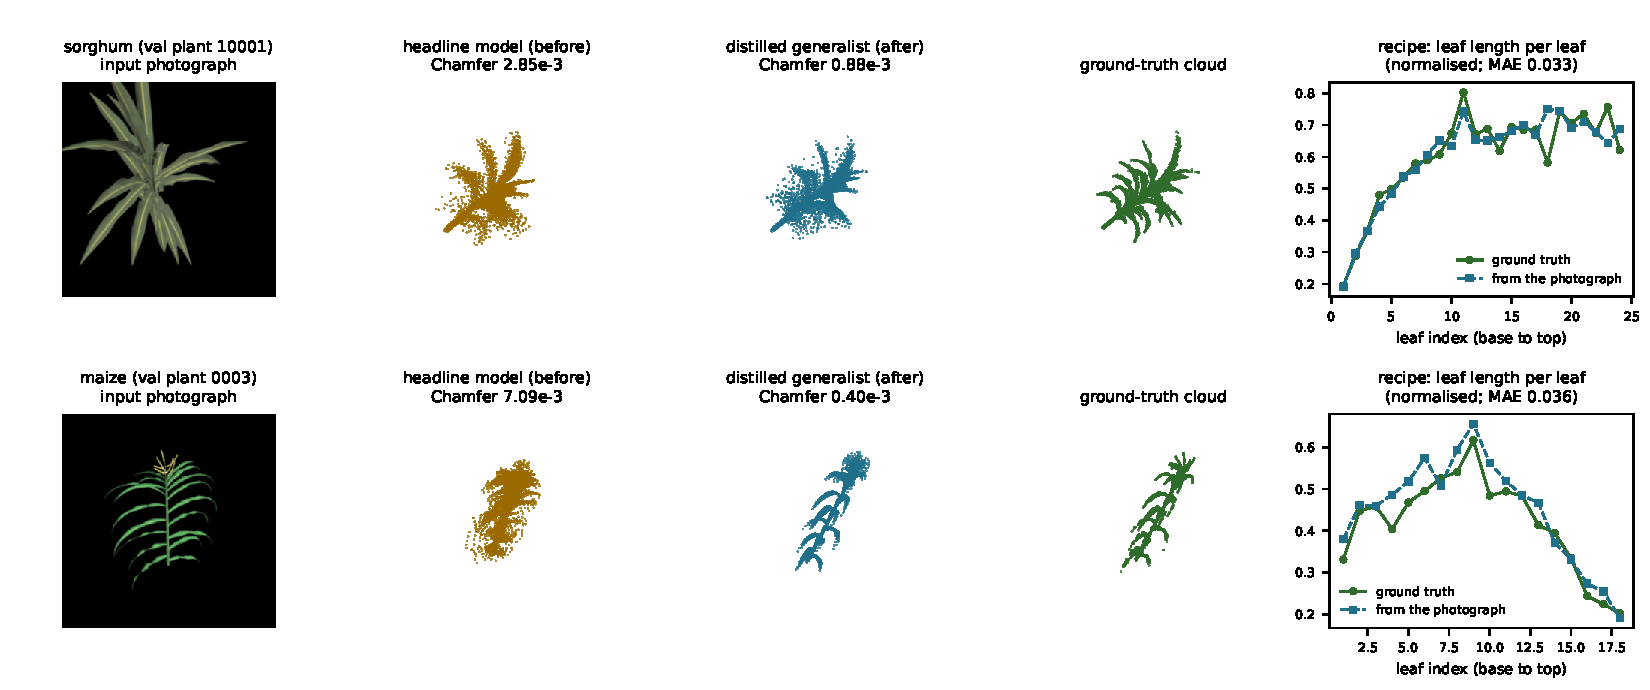
\includegraphics[width=\linewidth]{Figures/fig_qual.pdf}
  \caption{\textbf{Single-photograph 3D plant reconstruction on held-out
  test plants.} Each row shows inference given only a single input
  photograph (left). The headline model before distillation and the
  distilled generalist generate 3D point clouds, with Chamfer distance
  indicated above. The rightmost panel demonstrates parameter recovery by
  comparing the generalist's recovered normalized leaf lengths with exact
  ground truth across leaf indices from base to top.}
  \label{fig:qual}
\end{figure*}

\begin{figure}[t]
  \centering
  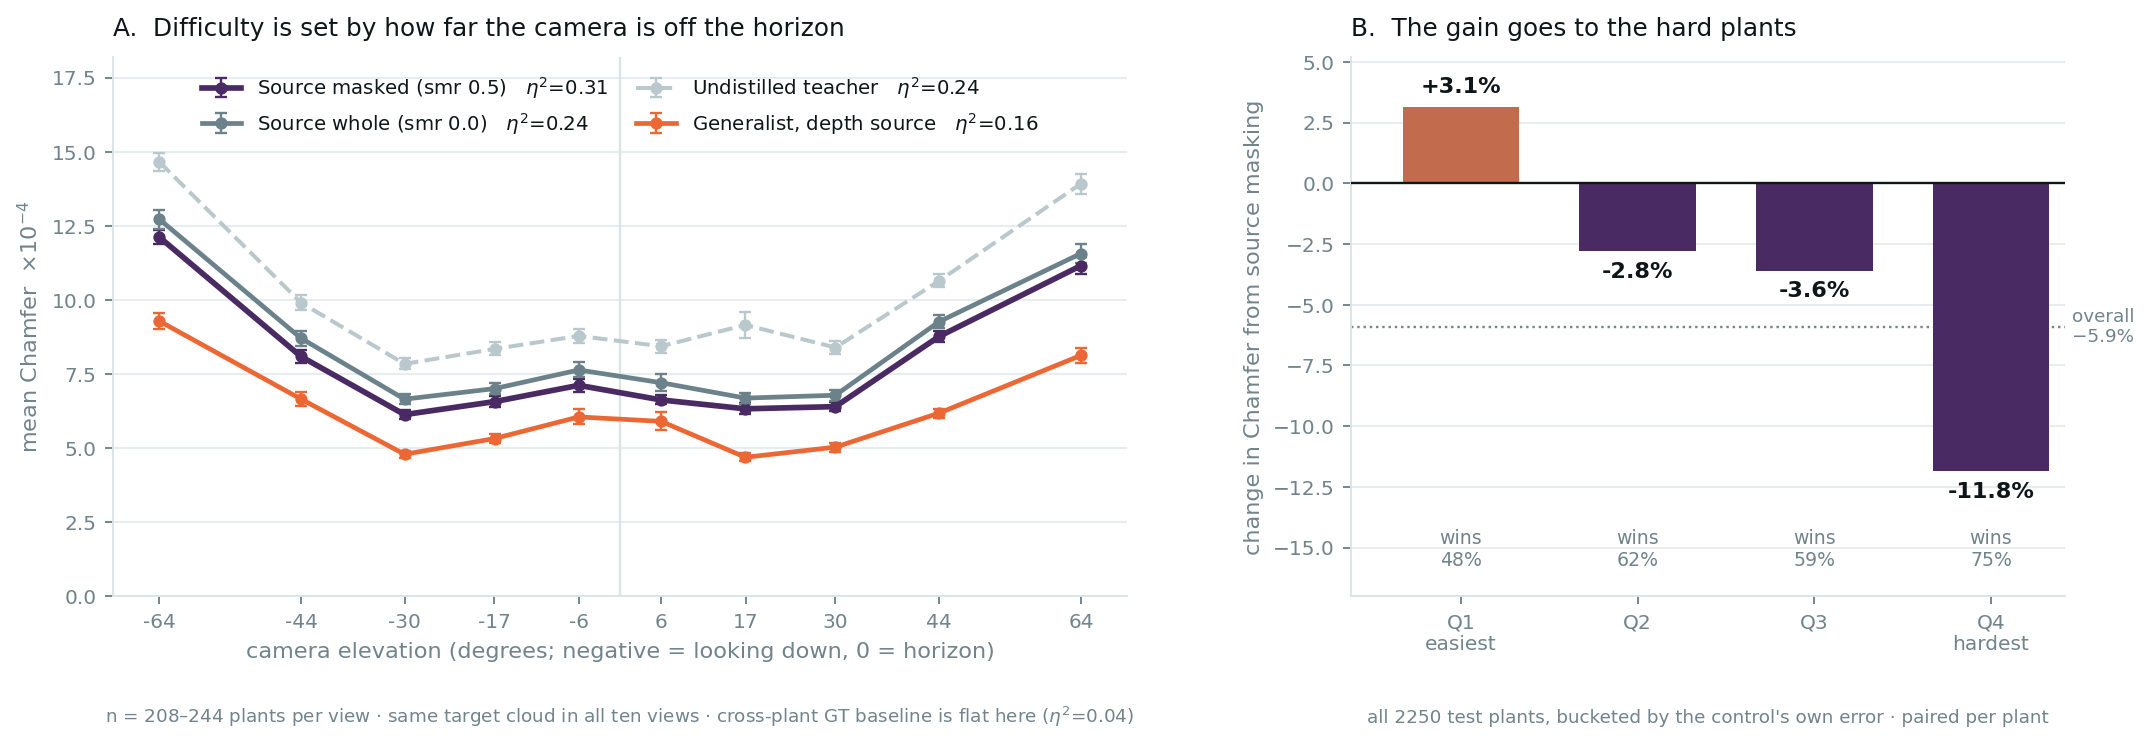
\includegraphics[width=\linewidth]{Figures/fig_view_elevation.png}
  \caption{\textbf{Viewpoint elevation determines reconstruction
  difficulty.} (A) Photograph-to-cloud Chamfer distance of test plants
  plotted by camera elevation angle (208--244 plants per elevation view). Pretrained and distilled single-sensor models follow a symmetric U-shaped
  error curve centered on horizontal side views; camera elevation accounts
  for $\eta^2 = 0.24\text{--}0.31$ of per-plant reconstruction variance. (B) Performance gain from masking 50\% of source tokens during
  distillation, grouped by error quartile of the control model,
  demonstrating concentrated improvement on challenging plant geometries.}
  \label{fig:views}
\end{figure}

\begin{figure}[t]
  \centering
  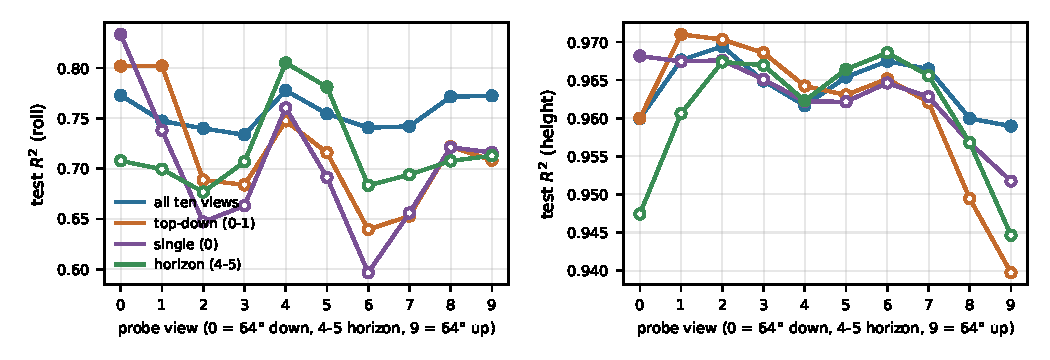
\includegraphics[width=\linewidth]{Figures/fig_e5_views.pdf}
  \caption{\textbf{Effect of training view distribution on downstream
  phenotype probing (sorghum test).} Probes are fitted and evaluated on
  individual views $k$ for model variants trained on all ten views versus
  restricted bands of the elevation ladder. Filled markers indicate
  training views. Restricted training view bands improve probe performance
  specifically within those elevations but degrade generalization on
  unobserved view angles.}
  \label{fig:e5views}
\end{figure}

\begin{figure}[t]
  \centering
  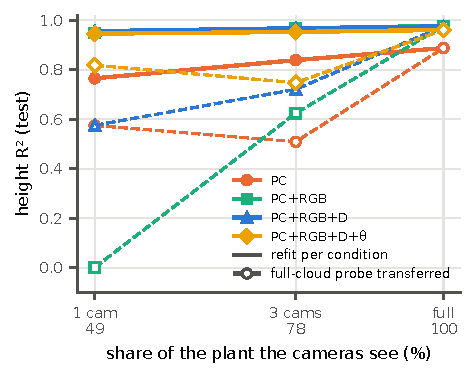
\includegraphics[width=\linewidth]{Figures/fig_partial_clouds.pdf}
  \caption{\textbf{Phenotypic information persistence under partial
  visibility.} Plant height prediction performance ($R^2$, test set)
  plotted against the visible percentage of the plant under 1-camera,
  3-camera, and full coverage. Solid lines represent probes refit per
  visibility condition; dashed lines show direct transfer of the
  full-cloud readout probe.}
  \label{fig:partial}
\end{figure}

\begin{figure}[t]
  \centering
  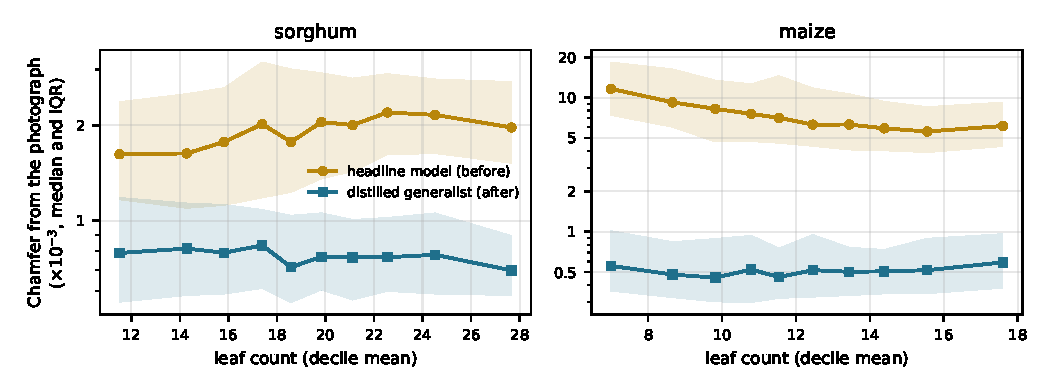
\includegraphics[width=\linewidth]{Figures/fig_leafcount.pdf}
  \caption{\textbf{Error against plant complexity (test, 2{,}250 plants per
  species).} Chamfer distance of point clouds generated from single
  photographs across leaf-count deciles for the headline model before
  distillation and the distilled generalist.}
  \label{fig:leafcount}
\end{figure}

\begin{figure*}[t]
  \centering
  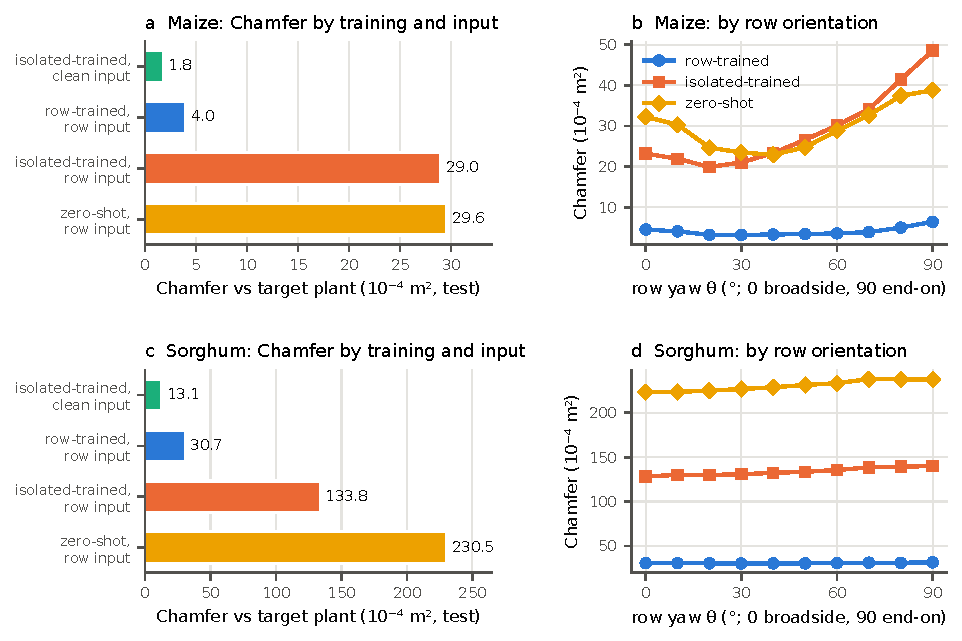
\includegraphics[width=\linewidth]{Figures/fig_rows.pdf}
  \caption{\textbf{Quantitative row occlusion performance on maize (a, b)
  and sorghum (c, d) test rows.} (a, c) Target plant Chamfer distance
  comparing isolated-trained models on clean versus row inputs, row-trained
  models on row inputs, and zero-shot baselines. (b, d) Reconstruction
  error plotted across row orientation yaw angles ($\theta$). Fine-tuning
  on row scenes eliminates the vast majority of neighbor-induced occlusion
  error in both species.}
  \label{fig:rows}\label{fig:row_reconstruction_quant}
\end{figure*}

\begin{figure*}[t]
  \centering
  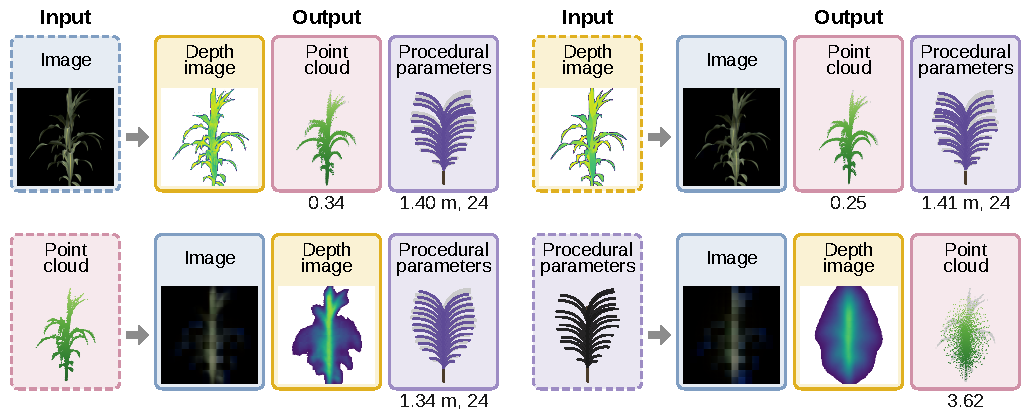
\includegraphics[width=\linewidth]{Figures/fig_any2all_sorghum_ugg.pdf}
  \caption{\textbf{Any-to-all, sorghum: each stream alone in, the other three out.} The distilled generalist on one held-out test plant. Each block gives it one stream (dashed box, left of the grey arrow) and shows the three streams it generates (solid boxes); the box color marks the stream: image blue, depth yellow, point cloud pink, procedural parameters purple. Generated point clouds and procedural parameters are drawn over the ground truth in grey, the parameters as a stem-and-leaves schematic. Under each generated point cloud: its Chamfer distance ($10^{-3}$); under each generated parameter set: height and leaf count (truth 1.43\,m, 24 leaves). The plant is selected for clarity among the test plants with the lowest image-to-cloud Chamfer, seen within $25^\circ$ of the horizon. The parameters alone give only a coarse plant (Chamfer 3.62 here, 6.83 on average in Table~\ref{tab:anysubset}).}
  \label{fig:any2any-sorghum}
\end{figure*}

\begin{figure*}[t]
  \centering
  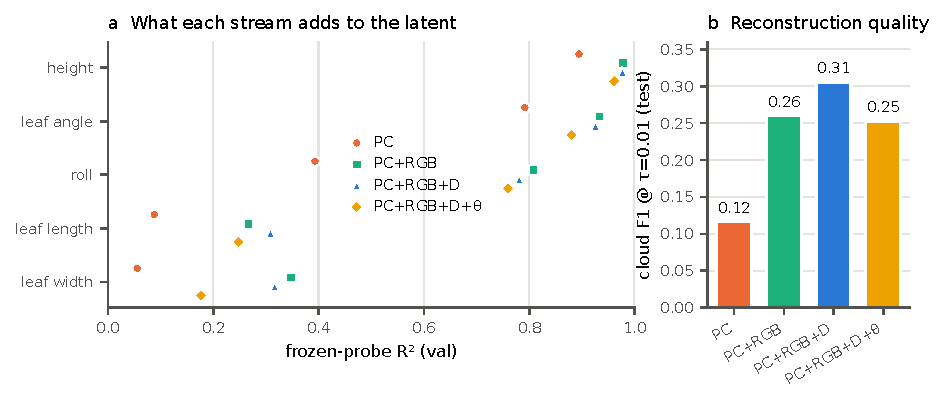
\includegraphics[width=\linewidth]{Figures/fig_e2_streams.pdf}
  \caption{\textbf{Modality contributions to latent representation and
  geometry reconstruction (sorghum).} (a) Frozen-probe $R^2$ across
  phenotypic traits. (b) Reconstruction $F_1$ score at threshold
  $\tau = 0.01$ ($\approx 1$\,cm).}
  \label{fig:stream_contributions}
\end{figure*}

\begin{figure*}[t]
  \centering
  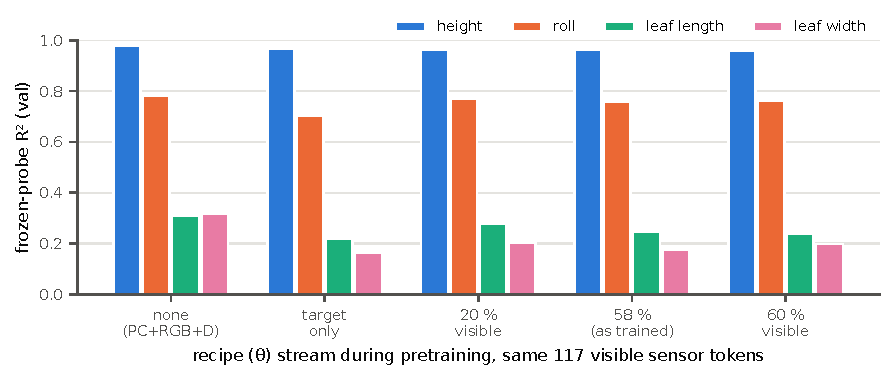
\includegraphics[width=\linewidth]{Figures/fig_param_controls.pdf}
  \caption{\textbf{Influence of procedural parameter stream visibility
  during pretraining.} Linear probe $R^2$ performance across parameter
  visibility levels under matched sensor token budgets.}
  \label{fig:controls}
\end{figure*}

\begin{figure}[t]
  \centering
  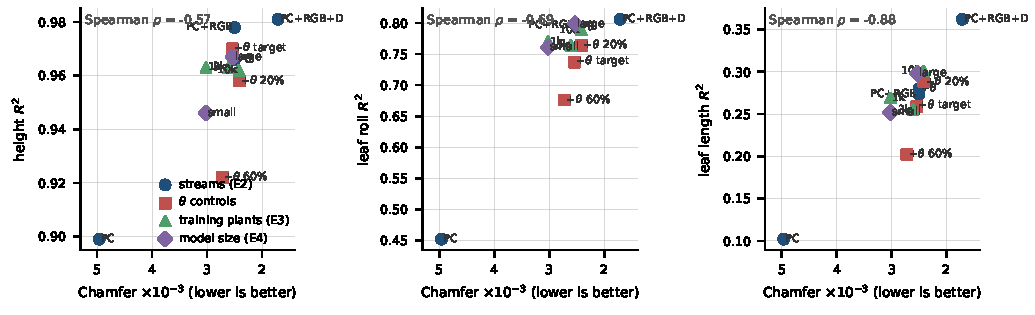
\includegraphics[width=\linewidth]{Figures/fig_metrics.pdf}
  \caption{\textbf{Divergence between Chamfer distance and frozen-latent
  probe metrics.} Validation Chamfer distance plotted against height probe
  $R^2$ across twelve model variants.}
  \label{fig:metrics}\label{fig:metric_divergence}
\end{figure}

\begin{figure*}[t]
  \centering
  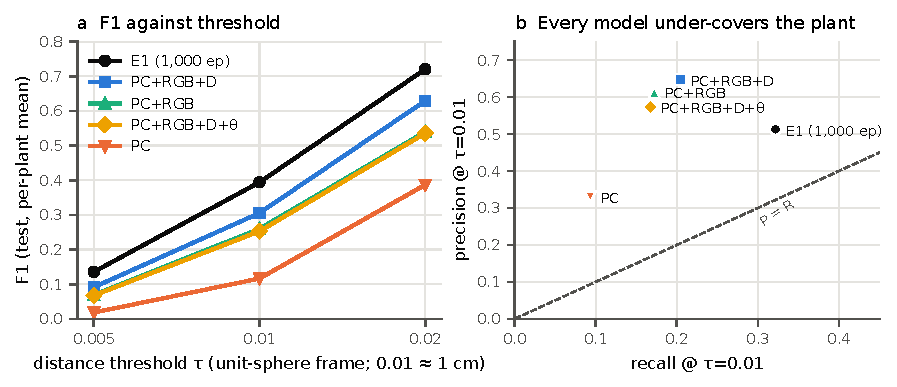
\includegraphics[width=\linewidth]{Figures/fig_fscore.pdf}
  \caption{\textbf{Point cloud completion precision, recall, and $F_1$
  evaluation (sorghum test).} (a) $F_1$ score against distance threshold
  $\tau$. (b) Precision vs. recall at $\tau = 0.01$.}
  \label{fig:fscore}\label{fig:precision_recall}
\end{figure*}

\begin{figure}[t]
  \centering
  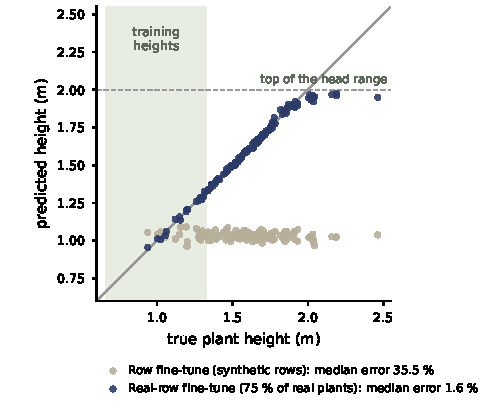
\includegraphics[width=0.92\columnwidth]{Figures/fig_e10_height.pdf}
  \caption{Predicted against true plant height on the 130 held-out real maize plants (median over each plant's 36 camera stops, all three streams in). Trained on synthetic rows only, the model writes about 1.03\,m for every plant; after fine-tuning on the other 75\% of the real plants it follows the true height up to the 2.0\,m end of the recipe's range. The shaded band is the training height range.}
  \label{fig:e10_height}
\end{figure}

\begin{figure*}[t]
  \centering
  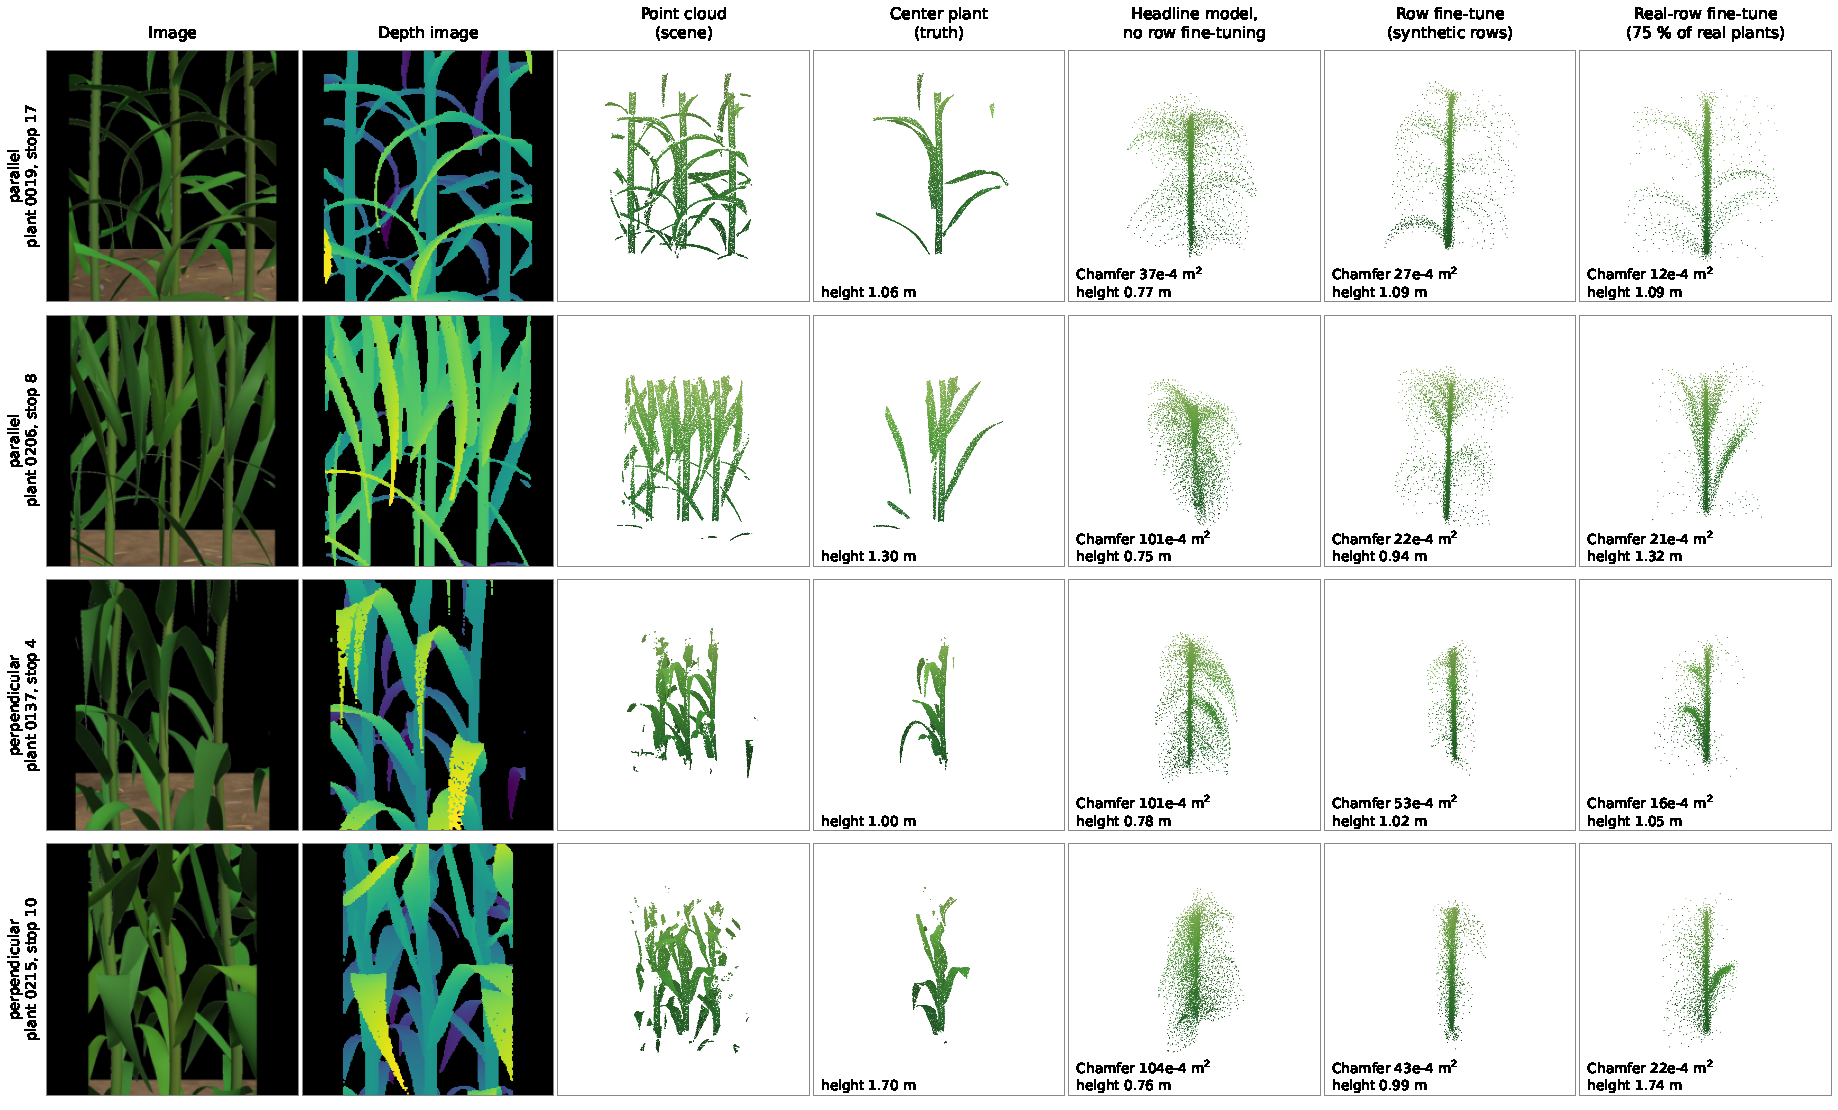
\includegraphics[width=\textwidth]{Figures/fig_e10_real.pdf}
  \caption{Real maize rows (E10), held-out test plants. Each row of panels is one camera stop on a crop row of a real maize plant that the real-row fine-tune never saw, in the parallel and perpendicular layouts, picked at its median Chamfer for the layout. From left: the image, depth image and scene point cloud the model reads, the center plant as the camera sees it, and the center plant written by the headline model without row fine-tuning, by the row fine-tune trained on synthetic rows, and by the real-row fine-tune trained on 75\% of the real plants, each with its Chamfer and predicted height. Row fine-tuning removes the neighbors; fine-tuning on real plants recovers the leaf layout and the height.}
  \label{fig:e10_real}
\end{figure*}

\begin{figure*}[t]
  \centering
  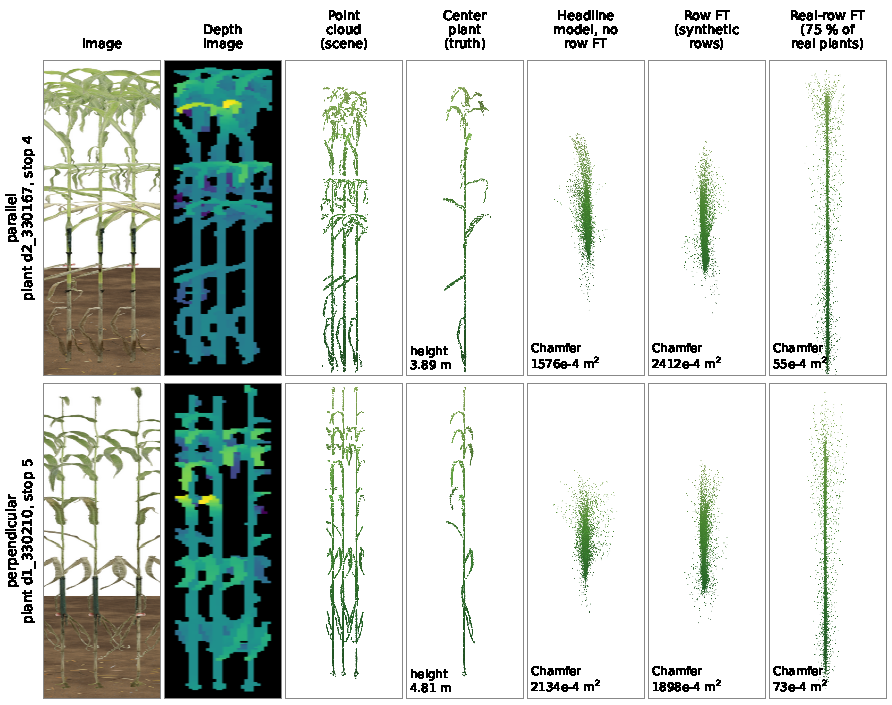
\includegraphics[width=0.62\textwidth]{Figures/fig_e10_real_sorghum.pdf}
  \caption{Real sorghum rows (E10), held-out test plants. Columns as in Fig.~\ref{fig:e10_real}; the image is the camera photograph, a tall strip framed to the whole plant. The plants are 2.2--5.3\,m tall; the stems of the training plants reach at most 1.74\,m. Without real data every model writes a short, dense plant; the real-row fine-tune, trained on 19 real plants, recovers the stalk over the full plant height but few of the leaves.}
  \label{fig:e10_real_sorghum}
\end{figure*}

\begin{figure*}[t]
  \centering
  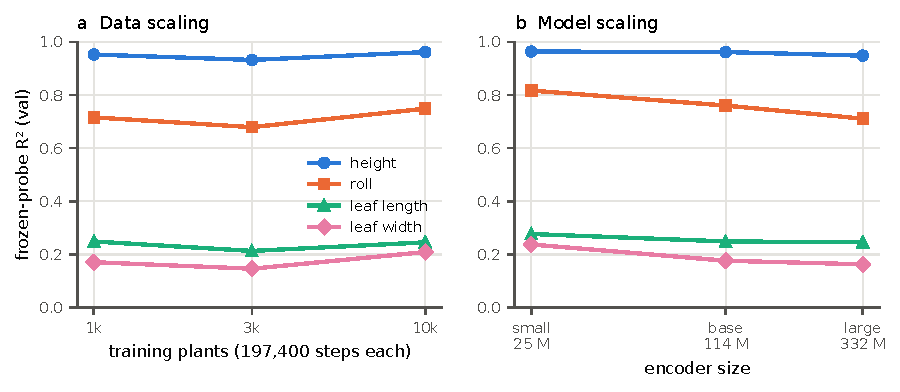
\includegraphics[width=\linewidth]{Figures/fig_scaling.pdf}
  \caption{\textbf{Dataset and model capacity scaling at equal step compute
  (sorghum).} Linear probe validation $R^2$ plotted against dataset size
  (a) and encoder parameter capacity (b).}
  \label{fig:data_model_scaling_fig}
\end{figure*}

\begin{figure}[t]
  \centering
  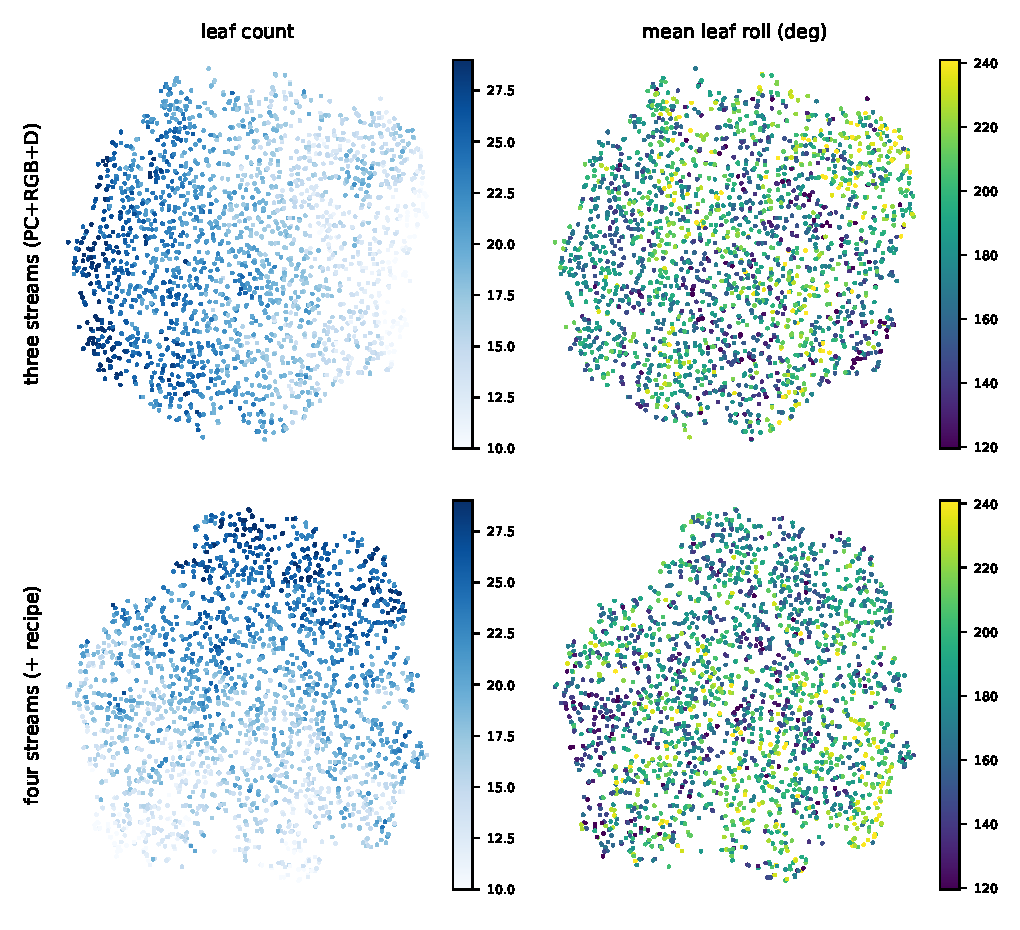
\includegraphics[width=\linewidth]{Figures/fig_e9_tsne.pdf}
  \caption{\textbf{Latent space visualization (sorghum validation set).}
  t-SNE projections of frozen encoder \texttt{[CLS]} tokens for 3-stream
  ($\mathrm{PC}+\mathrm{RGB}+\mathrm{D}$) and 4-stream ($+\theta$) models,
  colored by plant leaf count and mean leaf roll.}
  \label{fig:tsne}\label{fig:latent_tsne}
\end{figure}

\section{Evaluation Metrics}
\label{app:metrics}

Geometry is symmetric squared Chamfer in the unit-sphere frame
($\times 10^{-3}$; 1.0 corresponds to $\approx 33$\,mm RMS on the median
sorghum plant and $\approx 19$\,mm on the median maize plant, with metric
scales measured per plant), evaluated in the masked regime of pretraining
for pretrained models and with unmasked inputs for distilled students.
Parameter accuracy is MAE over normalized $[0,1]$ fields of hidden,
non-padding leaf tokens, reported as trait \emph{skill} where informative,
\begin{equation}
  \mathrm{Skill} = 1 - \frac{\mathrm{MAE}}{\mathrm{MAE}_{\text{mean}}},
  \label{eq:trait-skill}
\end{equation}
so that 1 is perfect recovery and 0 matches predicting the dataset
mean. Representation quality is the probe protocol of Sec.~\ref{sec:method}, $R^2$
with 95\% paired-bootstrap intervals on 2{,}250 validation and 2{,}250 test
plants. Sorghum's four named developmental traits have effective rank two
(height and leaf count couple at $r = 0.994$), so sorghum probing adds the
generator's independent axes (leaf roll, blade length); maize's eleven
traits are largely independent.

\section{Encoder-Comparison Probe Protocol}
\label{app:probe}

\noindent\textbf{Probe protocol for the encoder comparison.}
Table~\ref{tab:baselines} applies the trait probe of Sec.~\ref{sec:method} to every encoder in the same way, with two changes that let the published encoders take part. First, each plant is represented by the mean of the encoder's output tokens, the one readout that every encoder supports; our models leave their \texttt{[CLS]} token out of this mean. Second, each encoder receives only the streams it was built for, all taken from view 00 of the plant: DINOv2 the photograph, MultiMAE the photograph and depth frame, Point-MAE the point cloud, EmbodiedMAE all three, and each \method{} encoder the sensor streams it was pretrained on. The procedural parameters are never an input. For each encoder and trait, the features of the 10{,}500 training plants are standardized with training statistics only. A ridge regression is then fitted, with its regularization strength chosen from $\{0.1, 1, 10, 10^2, 10^3, 10^4\}$ by five-fold cross-validation on the training plants. The table reports $R^2$ on the 2{,}250 validation plants. The network trained from scratch on the labels goes through the same probe on its frozen features; its own regression head is not used. The traits are the generator's ground truth for each plant. In sorghum they are stem length, leaf count, mean leaf branching angle, mean leaf roll and mean leaf length. In maize they are summed stem internode length, mean leaf angle, mean leaf curvature and stem radius. The validation and test splits are enriched with extreme plants, with about 1.8 times the training variance in sorghum and 1.5 to 2.6 times in maize. The $R^2$ values therefore rank the encoders within the table, but they are not comparable with values reported in other work. Test $R^2$ stays close to validation; for the maize headline model, height reaches $0.747$ on validation and $0.759$ on test.

\noindent\textbf{Camera pose artifact analysis.}
Evaluating Point-MAE with full camera pose matrices yields strong maize
performance. However, this is largely a synthetic renderer artifact:
synthetic maize renders place leaf planes along a canonical world plane, so
camera pose matrices leak plant azimuth orientation. Evaluating Point-MAE
with gravity-only camera poses (realistic field calibration) reduces
performance ($R^2$ drops from $0.720$ to $0.588$ on height), while
\method{} performance remains unaffected.

\section{Extended Discussion}
\label{app:discussion}

The discussion of Sec.~\ref{sec:discussion}, in full.

We discuss the core insights, metric divergences, architectural principles,
and limitations established by our experiments.

\noindent\textbf{Privileged parameter visibility and modality competition.}
A central design question in multimodal architectures trained alongside
generative models is where privileged structural information should enter
the network. The procedural parameter stream $\theta$ is the only modality
that states target phenotypic traits verbatim, yet it is never available at
deployment in the field. Across our controlled ablations
(Sec.~\ref{sec:exp-params}), exposing parameter tokens to the encoder
during pretraining degraded the quality of learned sensor representations
in both sorghum and maize. In sorghum, every model arm that saw parameter
tokens in the encoder learned inferior visual features, with the
degradation on the size traits growing with the stream's visibility
(Tab.~\ref{tab:token_budget}).

This behavior can be understood through the lenses of shortcut learning,
modality competition~\citep{peng2022ogm}, and negative gradient
transfer~\citep{yu2020pcgrad}. When ground-truth parameter tokens are
visible to the transformer encoder, they directly encode target geometry. A
plausible account is that the encoder learns a low-cost shortcut through
these parameter tokens, starving the visual (RGB, depth) and point cloud
streams of gradient updates; when parameter tokens are then absent at
inference, the sensor representations prove impoverished.

The species-specific control arms (Tab.~\ref{tab:token_budget}) reveal an
additional nuance:
\begin{itemize}
\item  \textbf{Sorghum}: Keeping parameter tokens strictly as a decoder
  target ($\rho_\theta = 1.0$) continues to lower sensor latent quality
  ($R^2$ drops from $0.977$ to $0.966$ on height). Sorghum morphological
  parameters are tightly coupled (effective rank two); a plausible
  mechanism is gradient competition during multi-task decoding that pulls
  sensor representations toward global plant size, the leading principal
  component of the sorghum latent. \item  \textbf{Maize}: Keeping parameters strictly as a decoder target
  ($\rho_\theta = 1.0$) or restricting visibility to 20\% improves sensor
  latent probing across all eleven traits ($R^2 = 0.776$ vs.\ $0.633$ on
  height). Maize parameters contain 11 independent morphological
  dimensions; supervising them as a generation target provides structured
  multi-task decoder gradients, consistent with a regularizing effect on
  sensor latents without encoder shortcuts.
\end{itemize}

These findings yield an architectural design rule for multimodal masked
autoencoders trained on synthetic or procedural data: \emph{privileged
generative parameters should never be largely visible to the encoder during
pretraining}. Setting parameter tokens strictly as a decoder reconstruction
target ($\rho_\theta = 1.0$) or applying heavy gating
($\rho_\theta \le 0.20$) prevents encoder shortcut learning while
preserving generative parameter output capabilities; whether the parameters
help even as a pure reconstruction target depends on the generator.

\noindent\textbf{Metric divergence on slender geometry.}
A critical empirical finding of this work is the structural divergence
between nearest-neighbor point cloud metrics (such as Chamfer distance) and
downstream phenotypic trait probing on slender geometry
(Sec.~\ref{sec:exp-metrics}, Fig.~\ref{fig:metric_divergence}). Standard
Chamfer distance evaluates surface proximity by computing average
nearest-neighbor point displacements:
\begin{equation}
  \mathrm{CD}(P, \hat P) = \frac{1}{|P|}\sum_{p\in P}\min_{q\in\hat P}\|p-q\|_2^2 + \frac{1}{|\hat P|}\sum_{q\in\hat P}\min_{p\in P}\|p-q\|_2^2.
  \label{eq:chamfer_def}
\end{equation}
Because crop organs (such as maize and sorghum leaves) are thin,
high-aspect-ratio surfaces, a predicted point cloud can achieve low Chamfer
distance simply by clustering points onto bulky central stalks while
omitting entire leaf blades. In contrast, downstream linear probes fitted
on frozen encoder embeddings directly measure whether latent
representations retain the structural parameter information required for
phenotyping.

Throughout our experiments, Chamfer distance and linear probes rank model
variants differently:
\begin{enumerate}
\item  \textbf{Depth stream addition}: Adding metric depth to RGB
  photographs reduces Chamfer distance by 28\% in sorghum and 25\% in
  maize, but yields negligible change in downstream probe $R^2$ scores
  (Tab.~\ref{tab:modality_value_add}). Depth ordering provides spatial
  surface proximity for decoders without expanding high-level trait
  information in the encoder. \item  \textbf{Data scaling}: Increasing pretraining dataset volume from
  1{,}000 to 10{,}000 plants reduces sorghum Chamfer error by 21\%
  ($3.13 \to 2.48 \times 10^{-3}$), whereas sorghum probe scores saturate
  by 10{,}000 plants (Tab.~\ref{tab:scaling_ablations}). \item  \textbf{Partial camera visibility}: Restricting point cloud inputs
  to a single camera perspective increases Chamfer error $2.6\times$ to
  $6.5\times$, whereas refitted linear probes of the fused arms lose at
  most $0.030$ in height $R^2$ (Tab.~\ref{tab:views}).
\end{enumerate}

These disagreements demonstrate that Chamfer distance alone is an
insufficient metric for evaluating slender 3D shape reconstruction. We
advocate evaluating structural downstream trait probes alongside Chamfer
distance, and incorporating distribution-matching losses (such as Sinkhorn
optimal transport divergence, Eq.~\eqref{eq:point-loss-sinkhorn}) during
training to force decoders to cover full organ geometry rather than
collapsing points onto central stalks.

\noindent\textbf{Partial coverage, camera viewpoint, and row occlusion.}
Sensor observations in agricultural field campaigns are inherently partial. Our experiments analyze three aspects of partial sensing:
\begin{itemize}
\item  \textbf{Viewpoint elevation dominance}: Across isolated camera
  perspectives, camera elevation angle dominates single-image
  reconstruction difficulty, accounting for $\eta^2 = 0.24\text{--}0.31$ of
  per-plant reconstruction variance (Fig.~\ref{fig:views}). Steep top-down
  and bottom-up perspectives suffer from severe self-occlusion where leaves
  stack vertically along the optical axis, whereas side-on views expose
  full blade silhouettes. \item  \textbf{Covariate shift under partial visibility}: While phenotypic
  trait information persists in encoder representations under partial
  surface coverage (refitted 1-camera height $R^2 = 0.960$), directly
  transferring linear probes trained on 100\% complete clouds to partial
  inputs results in performance failure ($R^2 \to -0.26$,
  Fig.~\ref{fig:partial}). Partial visibility induces a systematic
  covariate shift in latent feature space. Consequently, downstream
  phenotyping readouts deployed in the field must be refit or calibrated on
  sensor-matched partial coverage inputs. \item  \textbf{Implicit row occlusion reasoning}: In planted rows,
  neighboring foliage accounts for up to two-thirds of input point clouds
  and pixel areas. Standard models trained on isolated plants suffer
  catastrophic failure under row occlusion because decoders attempt to
  incorporate neighboring leaves into target plant reconstructions
  (Tab.~\ref{tab:regime_3}). Fine-tuning decoders to predict target main
  plant geometry behind occluding neighbors removes 92\% of
  neighbor-induced occlusion error in maize and 85\% in sorghum, forcing
  the network to perform implicit occlusion reasoning and segment target
  organs from inter-plant contact foliage.
\end{itemize}

Importantly, procedural parameter outputs ($\hat\theta$) demonstrate
superior robustness to partial visibility compared to raw point cloud
completions. Because the procedural generator $G(\hat\theta)$ acts as an
explicit biological prior, re-rendered procedural meshes generate complete
3D geometry even when input sensor observations capture only a fraction of
the plant surface.

\noindent\textbf{Capabilities and boundaries of cross-modal distillation.}
Cross-modal teacher--student distillation (Sec.~\ref{sec:method-distill})
converts a multimodal pretraining artifact into a fast, deployable
single-sensor inference model. Distilling a full-modality teacher
($\mathrm{RGB}+\mathrm{D}+\mathrm{PC}+\theta$) into single-sensor student
networks reduces overall cross-modal generation loss by 30.2\% in sorghum
and 43.5\% in maize (Tab.~\ref{tab:anysubset}). Distillation gains are
concentrated on the weakest input modalities (photograph-to-cloud Chamfer
error falls by 61\%) and the most challenging plant geometries
(Fig.~\ref{fig:views}B). Furthermore, supervising student models across all
four decoder targets simultaneously outperforms a specialized
parameter-only regression student (recipe MAE from the point cloud
0.019 against 0.036 and 0.038 for specialists trained at $10^{-4}$ and
$3 \times 10^{-5}$, from the same warm start at 0.040), consistent with
auxiliary visual reconstruction tasks acting as regularizing gradients for
parameter regression.

However, distillation exhibits clear boundary limits:
\begin{enumerate}
\item  \textbf{Viewpoint robustness}: Distillation lowers absolute
  reconstruction error across all camera views but does not flatten the
  U-shaped elevation difficulty curve (Fig.~\ref{fig:views}A). Viewpoint
  robustness cannot be acquired purely through distillation; it requires
  balanced elevation sampling during pretraining data capture
  (Fig.~\ref{fig:e5views}). \item  \textbf{Unobservable parameter instability}: Parameterizations
  submitted to inverse regression must be restricted to traits that field
  sensors can physically resolve. In early experimental iterations
  containing unobservable leaf waviness parameters, distillation caused
  these unconstrained parameter heads to develop severe view-dependent
  instability without improving trait skill (skill $\approx 0$). Restricting procedural parameter representations to observable
  physiological attributes (insertion heights, blade lengths, widths,
  angles, and rolls) ensures stable cross-modal distillation.
\end{enumerate}

\noindent\textbf{Limitations and future directions.}
We acknowledge several limitations in our current study:
\begin{itemize}
\item  \textbf{Single-seed ablation budgets}: Controlled ablation
  experiments (Tabs.~\ref{tab:modality_value_add} and~\ref{tab:token_budget})
  were executed under a standardized compute budget of 197{,}400 optimizer
  steps using a single seed per arm. Run-to-run baseline variance estimated
  from near-duplicate runs is $\approx 2\%$ in Chamfer distance and
  $\le 0.011$ in probe $R^2$; the non-monotone maize scaling differences,
  though significant under the paired bootstrap, could still reflect
  run-to-run variance. \item  \textbf{Procedural generator expressivity boundaries}: An inherent
  limitation of inverse procedural modeling is that recovered
  representations are bounded by the expressivity of the underlying
  generator $G$. If a physical plant exhibits morphological deformations
  unrepresented in $G$ (such as severe disease lesions, structural
  breakage, or tassel droop, which the generator renders without learnable
  variation), the framework fits the nearest valid procedural parameter
  configuration. Expanding procedural generators to support broader
  developmental malformations represents an important avenue for future
  research. \item  \textbf{Synthetic renderer regularities}: Synthetic rendering
  pipelines can introduce unintended canonical cues (such as fixed leaf
  plane azimuth alignments) that pose-aware baselines may exploit as
  shortcuts. Rigorous evaluation on real-world field captures
  (Sec.~\ref{sec:exp-real}) remains essential to verify true sim-to-real
  domain transfer.
\end{itemize}

By releasing \dataset{} (comprising 30{,}000 synthetic plants across maize
and sorghum with paired multimodal captures, physically simulated row
occlusion, and exact procedural parameter ground truth), we aim to provide
the 3D vision and digital agriculture communities with a benchmark for
evaluating multimodal completion and inverse procedural modeling on
slender, heavily occluded geometry.
%%%%%%%%%%%%%%%%%%%%%%%%%%%%%%%%%%%%%%%%%%%%%%%%%%%%%%%%%%%%%%%%%%%%%%%%%%%
% ==== end sec/5_discussion.tex ====
%%%%%%%%%%%%%%%%%%%%%%%%%%%%%%%%%%%%%%%%%%%%%%%%%%%%%%%%%%%%%%%%%%%%%%%%%%%
%%%%%%%%%%%%%%%%%%%%%%%%%%%%%%%%%%%%%%%%%%%%%%%%%%%%%%%%%%%%%%%%%%%%%%%%%%%
% ==== sec/6_conclution.tex (inlined) ====
%%%%%%%%%%%%%%%%%%%%%%%%%%%%%%%%%%%%%%%%%%%%%%%%%%%%%%%%%%%%%%%%%%%%%%%%%%%

\section{Detailed Literature Review}
\label{app:litreview}

This appendix expands the compressed related-work discussion of
Section~\ref{sec:related} across six core bodies of literature on which
\method{} builds and from which it departs.

\subsection{Procedural plant models and inverse procedural modeling}
Procedural modeling of plant architecture originated with Lindenmayer
systems (L-systems)~\citep{prusin1990abop} and matured into parametric
generators whose parameters encode physiologically meaningful organ-level
attributes~\citep{floraforge2026,hadadi2025procmaize}. Inverting such
models, recovering generative parameters from visual observations, has a
long history for woody trees: Stava et al.\ fit tree generator parameters
via stochastic search~\citep{stava2014ipmtrees}, Talton et al.\ formulated
inverse procedural modeling as Markov Chain Monte Carlo (MCMC)
inference~\citep{talton2011metropolis}, and Guo et al.\ inferred structural
L-systems from 3D point clouds~\citep{guo2020ipmlsys}, with deep generative
variants following~\citep{latentlsys2023}.

These methods optimize parameters on a per-instance basis. None performs
amortized, single-forward-pass inversion of a procedural plant generator
from noisy, field-degraded sensor data. The closest feed-forward precedents
lie outside agriculture: shape-program
induction~\citep{shapeprograms2019}, diffusion-based inverse procedural
content generation from single photographs~\citep{zhao2025dipcg},
text-conditioned CAD generation~\citep{text2cad2024}, and cadrille, which
maps images, point clouds, or text to executable CAD
programs~\citep{kolodiazhnyi2025cadrille}. However, these systems operate
on rigid, clean, isolated man-made objects. None addresses deformable
slender organs, heavy inter-plant row occlusion, or real-world sensor
noise, and none investigates whether continuous program parameters should
enter the transformer encoder during multimodal pretraining.

\subsection{Learned parametric recovery of crop plants}
Recent systems attempt to recover parametric plant models from 3D scans. Demeter learns a joint morphology model (topology, articulation, and PCA
surface variations) from soybean point clouds~\citep{demeter2025}, while
Ghrer et al.\ infer grammar-style parameterized crop representations from
3D laser scans~\citep{ghrer2025paramplants}. Both systems assume a single,
clean, highly complete point cloud as input, and neither addresses missing
sensor modalities or inter-plant row occlusion.

CropCraft recovers procedural crop structure by applying Bayesian
optimization over procedural parameters matched against multi-view NeRF
depth maps~\citep{cropcraft2026}; however, per-scene optimization requires
substantial computation per plant. A staged annotation pipeline processes
terrestrial laser scans through vision-language model prompting and fits
procedural NURBS descriptors via differentiable
refinement~\citep{hadadi2026vlmmaize,hadadi2025procmaize,nurbsdiff2022},
requiring $\sim 10$ minutes of computation per isolated plant. Tree-D
Fusion reconstructs simulation-ready urban trees from street-level imagery
via diffusion priors~\citep{lee2024treedfusion}, but its
envelope-then-branch pipeline targets woody tree silhouettes rather than
thin, deformable agricultural crop blades.

\subsection{Point cloud completion and slender geometry}
Learned point cloud completion has advanced from folding-based
decoders~\citep{yuan2018pcn} to geometry-aware
transformers~\citep{yu2021pointr,yu2023adapointr} and
extrapolation--interpolation architectures~\citep{cai2024einet}. Standard
benchmarks (e.g., PCN, ShapeNet-55/34) consist of compact, largely convex
rigid objects and contain no slender-under-occlusion categories. Standard
completion algorithms assume missing geometry represents self-occluded
object surfaces without severe inter-object clutter.

Plant-specific completion has recently emerged, including amodal
segmentation and geometry completion for occluded
crops~\citep{lee2026occ}. However, these methods output unstructured point
clouds rather than editable, biologically interpretable procedural
parameters. Curve-aware and thin-structure reconstruction
methods~\citep{curvegaussian2025,qi2026rethinking} address slender
geometry, a regime in which standard Chamfer distance fails due to
structural insensitivity to thin
surfaces~\citep{wu2021dcd,song2026structural}. This limitation has
motivated density-aware and information-theoretic distance
variants~\citep{wu2021dcd,lin2023infocd}. In this work, we systematically
compare surface geometric metrics against downstream linear trait probes on
frozen encoder latents, demonstrating that the two metrics rank
architectural choices differently on slender plant geometry.

\subsection{3D plant phenotyping}
Organ-level 3D phenotyping datasets, including Pheno4D's annotated maize
and tomato temporal sequences~\citep{schunck2021pheno4d},
Crops3D~\citep{crops3d2024}, and field-scale maize scans carrying
procedural reference fits~\citep{maizefield3d2025}, support trait
extraction using deep point cloud
architectures~\citep{qi2017pointnet,qi2017pointnetpp}. Furthermore,
field-based radiance-field capture is increasingly
viable~\citep{arshad2024nerf_field}. However, no existing benchmark
combines real-field captures, slender plant geometry, physically simulated
inter-plant row occlusion, and exact procedural ground-truth parameter
targets across multiple crop species. \dataset{} is designed to fill this
gap.

\subsection{Multimodal masked pretraining and distillation}
Masked autoencoding~\citep{he2022mae} has been extended to multimodal
domains: MultiMAE over RGB, depth, and semantic
segmentation~\citep{bachmann2022multimae}; 4M and 4M-21 over tokenized
visual, structural, and textual
modalities~\citep{mizrahi2023fourm,bachmann2024fourm21}; Point-MAE over 3D
point clouds~\citep{pang2022pointmae}; and EmbodiedMAE over RGB, depth, and
point clouds for robotic manipulation~\citep{dong2025embodiedmae}.

Maintaining robustness under missing input modalities is an active area of
research~\citep{wang2024robustmissing}. Cross-modal feature distillation
from multi-sensor teacher models to single-sensor student models is
established for discriminative tasks~\citep{hinton2015distillation}. We
extend cross-modal distillation to a \emph{generative} setting for
structured parameter regression, encoding continuous procedural parameters
as numerical tokens via xVal-style embedding~\citep{golkar2023xval}. Our
finding that exposing ground-truth parameter tokens to the encoder degrades
visual representation quality connects to modality
competition~\citep{peng2022ogm} and gradient
interference~\citep{yu2020pcgrad,chen2018gradnorm}, establishing a concrete
design rule for privileged generative modalities in multimodal pretraining.

\subsection{Synthetic-data pretraining and sim-to-real transfer}
Pretraining deep representations on synthetic data is established across
domains ranging from fractal geometry~\citep{kataoka2020fractaldb} to
procedural 3D environments~\citep{raistrick2023infinigen,greff2022kubric},
with domain randomization closing the sim-to-real
gap~\citep{tobin2017domainrand}. The utility of synthetic data is known to
depend heavily on downstream task alignment~\citep{fan2023intriguing}, and
model self-consumption presents documented stability
risks~\citep{alemohammad2023mad}.

Our setting represents an ideal use-case for synthetic pretraining: the
deployment target is the exact parameter space of the procedural generator,
the generator spans the continuous morphological variation of target crop
species, and the framework is validated against high-density real-world
field captures~\citep{maizefield3d2025}.

% =========================================================================
\section{Detailed Ablation Studies}
\label{app:ablations}

All reported ablation experiments are evaluated on the complete validation
and test sets of both species across standardized $197{,}400$ optimizer
step budgets at global batch size 32. Representation quality is evaluated
using ridge regression probes fit on frozen \texttt{[CLS]} tokens (one
deterministic perspective per plant) with paired bootstrap confidence
intervals (2{,}000 resamples over plants). A performance difference is
classified as significant only when its 95\% confidence interval excludes
zero on both validation and test splits simultaneously.

\subsection{Training view distribution}
\label{app:views-full}

We pretrain models under restricted camera elevation bands: top-down views
($i \in \{0,1\}$), horizontal views ($i \in \{4,5\}$), or a single top-down
view ($i=0$), benchmarked against pretraining across all ten views. Probes
are evaluated across held-out views $k$ (Fig.~\ref{fig:e5views}). Restricted models achieve superior performance on their specific training
elevations (e.g., $+0.061$ roll $R^2$ on view 0 for the single-view model),
but experience performance drops on unobserved elevations (falling by
$-0.066$ to $-0.144$ on distant views). Models trained on the complete
elevation ladder maintain stable performance across all perspective angles
($R^2 = 0.734\text{--}0.778$). Maize gives the same answer without a
per-view probe: its cameras sit at random elevations, so the probe camera is a
random one in every arm. All three restricted arms lose to the all-view arm on
every target (validation $R^2$ for height 0.45, 0.49 and 0.52 against 0.64 for
the top-down, horizontal and single-camera arms; leaf angle 0.82, 0.80 and 0.89
against 0.92; stem radius 0.57, 0.57 and 0.72 against 0.75). The single-camera
arm trains on one tenth of the images but at the probe's elevation distribution
and loses least; the two band arms train on twice as many images inside a band
and lose most, so covering the evaluation elevations matters more than the
number of images. Paired bootstraps over plants confirm it: against the
all-view arm the horizontal arm loses all 11 probe targets and the top-down and
single-camera arms lose 10 (height $-0.15$, $-0.19$ and $-0.12$ on validation,
95\,\% intervals of about $\pm 0.02$); no restricted arm wins a target.
Reconstruction gives the same reading through the point-cloud $F_1$
(protocol of Fig.~\ref{fig:precision_recall}, $\tau = 0.01$, test split). In
sorghum the score is taken on view 0, a top-down camera: the two arms trained
on that elevation reach 0.27 and 0.28 against 0.25 for the all-view arm, while
the horizontal arm, which never saw such a camera, falls to 0.03. In maize the
score is taken on a random camera, and every restricted arm falls below the
all-view arm's 0.31 (horizontal 0.22, top-down 0.19, single camera 0.17).

\subsection{Modality value-add ablations (E2)}
Eight pretraining arms per species were evaluated under identical optimizer
step budgets, differing strictly in active token streams
(Tab.~\ref{tab:supp-e2}).

\begin{table*}[t]
  \caption{\textbf{Extended modality value-add ablations (E2, validation
set).} In sorghum, including parameter tokens in the encoder increases
Chamfer error across sensor sets (except $\mathrm{PC}$ alone) and degrades
linear probe $R^2$. In maize, parameter inclusion lowers surface Chamfer
distance while its impact on probing depends on the sensor set.}
\label{tab:supp-e2}
\centering\small
\begin{tabular}{lcccc}
\toprule
 & \multicolumn{2}{c}{Sorghum} & \multicolumn{2}{c}{Maize} \\
Experimental Variant & Chamfer ($\times10^{-3}$) & Height $R^2$ & Chamfer ($\times10^{-3}$) & Height $R^2$ \\
\midrule
Point Cloud ($\mathrm{PC}$) & 5.00 & 0.895 & 2.63 & 0.171 \\
$\mathrm{PC} + \text{Depth}$ & 2.45 & 0.976 & 2.55 & 0.453 \\
$\mathrm{PC} + \text{RGB}$ & 2.57 & 0.979 & 1.61 & 0.620 \\
$\mathrm{PC} + \text{RGB} + \text{Depth}$ & 1.85 & 0.977 & 1.21 & 0.633 \\
$\mathrm{PC} + \text{Parameters } (\theta)$ & 4.84 & 0.860 & 2.49 & 0.256 \\
$\mathrm{PC} + \text{Depth} + \theta$ & 4.08 & 0.907 & 2.54 & 0.382 \\
$\mathrm{PC} + \text{RGB} + \theta$ & 3.00 & 0.962 & 1.21 & 0.509 \\
Full Four-Stream Model ($\mathrm{PC} + \text{RGB} + \text{Depth} + \theta$) & 2.53 & 0.962 & 0.99 & 0.635 \\
\bottomrule
\end{tabular}

\end{table*}

\subsection{Token-budget control arms}
In default four-stream pretraining, sensor streams share a total visible
budget of 122--123 tokens with parameter tokens (yielding 107.4 visible
sensor tokens vs.\ 117.0 in three-stream models, with parameter tokens
$\sim 58\%$ visible). Control arms decouple parameter tokens from the
sensor token allocation, restoring a full 117.0 visible sensor token
allocation across three parameter visibility levels: 20\%, 60\%, and 0\%
(target-only).

In sorghum, restoring sensor token budgets does not recover three-stream
probing performance: height $R^2$ remains $0.959\text{--}0.966$ (vs.\
$0.977$), and leaf roll $R^2$ remains $0.702\text{--}0.771$ (vs.\
$0.781$). In maize, 20\% parameter visibility and target-only parameter
supervision outperform both the shared-budget four-stream model and
three-stream $\mathrm{PC}+\mathrm{RGB}+\mathrm{D}$ across all eleven traits
on both splits.

\subsection{Parameters as a decoder reconstruction target only}
Restricting procedural parameters strictly to a decoder reconstruction
target ($\rho_\theta = 1.0$, never encoded as input) still degrades sensor
representations in sorghum relative to omitting the stream: height $R^2$
drops by $-0.011$, leaf roll by $-0.07$, mean leaf length by $-0.10$, and
leaf width by $-0.15$ on validation. The learned latent space becomes
heavily dominated by global plant scale: the first principal component
accounts for 44\% of total latent variance and correlates strongly with
leaf count ($|r| = 0.95$), while the participation ratio drops to 4.3
(vs.\ 6.7 for $\mathrm{PC}+\mathrm{RGB}+\mathrm{D}$). Conversely, in maize,
target-only parameter supervision ($\rho_\theta = 1.0$) yields the
top-performing four-stream model, outperforming
$\mathrm{PC}+\mathrm{RGB}+\mathrm{D}$ across all eleven traits.

\subsection{Data volume and model capacity scaling at fixed compute}
Table~\ref{tab:supp-scaling} evaluates dataset volume scaling ($1$k, $3$k,
$10$k, $10.5$k plants) and model parameter capacity (ViT-Small 25\,M,
ViT-Base 114\,M, ViT-Large 332\,M) under matched $197{,}400$ optimizer step
budgets.

\begin{table*}[t]
  \caption{\textbf{Extended data and model scaling metrics (validation
set).} Four-stream model evaluated across dataset sizes and encoder
capacities at equal $197{,}400$ optimizer step budgets. Scaling to
ViT-Large helps neither species at this budget; ViT-Small wins sorghum
roll and leaf length.}
\label{tab:supp-scaling}
\centering\small
\begin{tabular}{lcccc}
\toprule
 & \multicolumn{2}{c}{Sorghum} & \multicolumn{2}{c}{Maize} \\
Dataset Scale / Model Capacity & Chamfer ($\times10^{-3}$) & Height $R^2$ & Chamfer ($\times10^{-3}$) & Height $R^2$ \\
\midrule
1{,}000 Plants & 3.13 & 0.952 & 3.54 & 0.393 \\
3{,}000 Plants & 2.86 & 0.932 & 1.46 & 0.524 \\
10{,}000 Plants & 2.48 & 0.962 & 0.87 & 0.427 \\
10{,}500 Plants (Full Dataset) & 2.53 & 0.962 & 0.99 & 0.635 \\
\midrule
ViT-Small (25\,M parameters) & 2.86 & 0.964 & 1.22 & 0.563 \\
ViT-Base (114\,M parameters) & 2.53 & 0.962 & 0.99 & 0.635 \\
ViT-Large (332\,M parameters) & 2.68 & 0.948 & 1.06 & 0.580 \\
\bottomrule
\end{tabular}

\end{table*}

\subsection{Distillation dynamics per source modality}
Distillation from the full-modality teacher reduces overall cross-modal
generation loss by 30.2\% in sorghum and 43.5\% in maize (evaluating
epoch-0 warm-start initialization against epoch-100 distilled students). Gains are concentrated on the weakest input modalities:
point-cloud-to-cloud Chamfer error in sorghum drops from
$5.48 \times 10^{-3}$ to $1.39 \times 10^{-3}$, parameter-only-to-cloud
Chamfer drops from $22.7 \times 10^{-3}$ to $6.83 \times 10^{-3}$, and
photograph-to-cloud Chamfer in maize falls from $11.3 \times 10^{-3}$ to
$0.77 \times 10^{-3}$. Parameter regression MAE from point clouds alone is
halved in sorghum ($0.040 \to 0.020$). The parameter-only specialist
was retrained on the final data from the same headline warm start with the
first-release recipe (point-cloud source, half of its tokens hidden, recipe
target only, 100 epochs), once at the generalist's learning rate of $10^{-4}$
and once at the first-release rate of $3 \times 10^{-5}$. Scored on the full
validation split with the point cloud fully visible, the specialists reach a
recipe MAE of 0.036 and 0.038 (warm start 0.040), the generalist 0.019: the
student that also generates the photograph, the depth frame and the cloud
recovers the recipe better than the student trained on the recipe alone, at
either learning rate.

\subsection{Label-free view invariance across camera perspectives}
Because ten camera perspectives per plant share identical ground-truth
procedural parameters, prediction variance across perspectives provides a
label-free metric of view invariance. Teacher--student distillation reduces
both absolute parameter error and prediction spread across camera views by
$\sim 50\%$ on fields with skill (insertion height error reduced by 59\%,
branching angle error reduced by 60\%). Zero-skill fields instead become
more view-dependent under distillation, as the head starts to track image
noise; the final generator drops those fields.

\subsection{Frozen-encoder baselines and pose cues}
On sorghum, three-stream \method{} ($\mathrm{PC}+\mathrm{RGB}+\mathrm{D}$)
outperforms all published self-supervised visual encoders
(DINOv2~\citep{oquab2024dinov2}, MultiMAE~\citep{bachmann2022multimae},
Point-MAE~\citep{pang2022pointmae}, and
EmbodiedMAE-B~\citep{dong2025embodiedmae}) across all traits. Paired over
plants against EmbodiedMAE-B, \method{} wins 8 of 9 targets (height $R^2$
$+0.005$, roll $+0.04$, leaf length $+0.08$, leaf width $+0.09$). On maize,
four-stream \method{} outperforms EmbodiedMAE-B on 10 of 11 traits.

Evaluating Point-MAE with full 3D camera pose matrices yields inflated
performance on synthetic maize due to a renderer artifact: synthetic maize
scenes align leaf planes along a canonical world plane, enabling full pose
matrices to leak plant azimuth orientation. Evaluating Point-MAE with
gravity-aligned camera poses (realistic field calibration) reduces its
height $R^2$ from $0.720$ to $0.588$, while pose-free \method{} wins 5 of 9
decided traits.

\subsection{Masked reconstruction against published encoders}
\label{sec:supp-recon}

Table~\ref{tab:baselines} compares frozen features. Table~\ref{tab:supp-recon} compares what the encoders that have a decoder reconstruct when part of the input is hidden, on the same 2{,}250 validation plants per species and view 00. Image block: the photograph and the depth image are given with 75\% of each image's 16-pixel patches hidden (MultiMAE's pretraining budget) and the point cloud hidden; MultiMAE-B is compared with the \method{} encoders that read images. Both models predict per-patch standardized color, so both are de-standardized with the true patch mean and variance, the usual MAE convention, and the photograph is scored by PSNR on the plant pixels of the hidden patches. Each model's normalized depth is mapped back with the two per-image numbers its own normalization used and scored in millimeters on the same pixels. Cloud block: the point cloud alone is given with 60\% of its point groups hidden (Point-MAE's pretraining ratio). Point-MAE copies the visible 40\% of the points into its output and is given the centers of the hidden groups, as in its pretraining; \method{} receives neither and generates the whole cloud. Prediction and truth are each subsampled to 2{,}048 points and compared in the unit-sphere frame by Chamfer and by precision, recall and F1 at $\tau = 0.01$ and $0.02$.

The three-stream \method{} encoder reconstructs hidden photograph patches better than MultiMAE in both species (28.0 against 24.7\,dB in sorghum, 19.7 against 14.4\,dB in maize); the headline model is below MultiMAE in sorghum (23.4\,dB) and above it in maize (18.1\,dB). Depth is \method{}'s weak stream under this protocol. MultiMAE is better in sorghum (RMSE 280 against 400--483\,mm), and the three-stream encoder only matches it in maize (216 against 215\,mm). A predictor that fills every hidden plant pixel with the mean depth of the visible plant pixels reaches 336\,mm in sorghum and 236\,mm in maize (300 plants), so in sorghum the \method{} depth reconstruction is worse than this trivial baseline. Point-MAE reconstructs the cloud far more closely (F1 at $\tau = 0.01$: 0.26 against at most 0.13 in sorghum, 0.52 against at most 0.16 in maize), which its copied visible points and given group centers explain in part. Among the \method{} encoders, the headline model reconstructs the cloud best in both species. Its precision at $\tau = 0.01$ is nearer Point-MAE's than its recall (sorghum 0.22 against 0.32, recall 0.10 against 0.22): it places points on the plant but misses part of it.

\begin{table}[t]
  \caption{\textbf{Masked reconstruction against published encoders (validation, 2{,}250 plants per species).} Image block: 75\% of the photograph and depth patches hidden, the point cloud hidden; PSNR (dB) on the plant pixels of the hidden patches; depth RMSE and MAE in mm on the same pixels. The last row fills hidden plant pixels with the mean depth of the visible ones (300 plants). Maize depth images are encoded per plant, so maize millimeters are approximate. Cloud block: the point cloud alone, 60\% of its groups hidden; Chamfer ($\times10^{-3}$, unit sphere) and F1 at two thresholds at 2{,}048 points per side. Point-MAE keeps the visible 40\% of the points and is given the hidden groups' centers; \method{} is given neither. The \method{} encoders are those of Table~\ref{tab:baselines} (epoch 600; headline epoch 1{,}000).}
  \label{tab:supp-recon}
  \centering\scriptsize
  \setlength{\tabcolsep}{3pt}
  \resizebox{\columnwidth}{!}{%
  \begin{tabular}{l ccc ccc}
    \toprule
    & \multicolumn{3}{c}{Sorghum} & \multicolumn{3}{c}{Maize} \\
    \cmidrule(lr){2-4}\cmidrule(lr){5-7}
    \emph{Image block} & PSNR $\uparrow$ & Depth RMSE $\downarrow$ & Depth MAE $\downarrow$ & PSNR $\uparrow$ & Depth RMSE $\downarrow$ & Depth MAE $\downarrow$ \\
    \midrule
    MultiMAE-B (RGB+D) & 24.7 & \textbf{280} & \textbf{184} & 14.4 & \textbf{215} & 150 \\
    \method{} PC+RGB+D & \textbf{28.0} & 423 & 245 & \textbf{19.7} & 216 & \textbf{145} \\
    \method{} four streams & 26.9 & 483 & 299 & 18.3 & 263 & 183 \\
    \method{} headline & 23.4 & 400 & 229 & 18.1 & 280 & 200 \\
    Mean visible plant depth & -- & 336 & 258 & -- & 236 & 174 \\
    \midrule
    \emph{Cloud block} & Chamfer $\downarrow$ & F1@0.01 $\uparrow$ & F1@0.02 $\uparrow$ & Chamfer $\downarrow$ & F1@0.01 $\uparrow$ & F1@0.02 $\uparrow$ \\
    \midrule
    Point-MAE (PC) & \textbf{1.14} & \textbf{0.257} & \textbf{0.645} & \textbf{0.67} & \textbf{0.516} & \textbf{0.826} \\
    \method{} PC only & 9.58 & 0.044 & 0.225 & 4.95 & 0.061 & 0.230 \\
    \method{} PC+RGB+D & 7.73 & 0.069 & 0.250 & 4.13 & 0.080 & 0.276 \\
    \method{} four streams & 8.50 & 0.067 & 0.251 & 4.57 & 0.071 & 0.267 \\
    \method{} headline & 5.93 & 0.134 & 0.351 & 2.94 & 0.161 & 0.431 \\
    \bottomrule
  \end{tabular}}
  
\end{table}

\subsection{Latent space structure analysis (E9)}
Frozen encoder \texttt{[CLS]} embedding spaces form continuous, smooth
manifolds without discrete clustering, as expected for continuous synthetic
generators (best silhouette coefficient $0.15\text{--}0.24$ at $k=2$,
adjusted Rand index $\approx 0.0$ against shape deciles, t-SNE
trustworthiness $0.95\text{--}0.99$). The latent effective participation
ratio is low: $4.4\text{--}6.3$ (out of 768 dimensions) in sorghum and
$6.7\text{--}11.3$ in maize. Explaining 90\% of latent variance requires
14--15 principal components in sorghum and 18--19 in maize. In sorghum, the
leading principal component aligns with global plant scale (correlation
with leaf count $|r| = 0.73\text{--}0.94$).

\subsection{Source of Occlusion}
\label{sec:abl_occ}

Rendering realistic occluded scenes is expensive, so we ask whether cheaper, synthetic occlusion can replace it
during training. We compare four sources of occlusion (\cref{fig:occ_sources}) and test every model on the same
rendered occluded scenes.

\begin{figure*}[t]
  \centering
  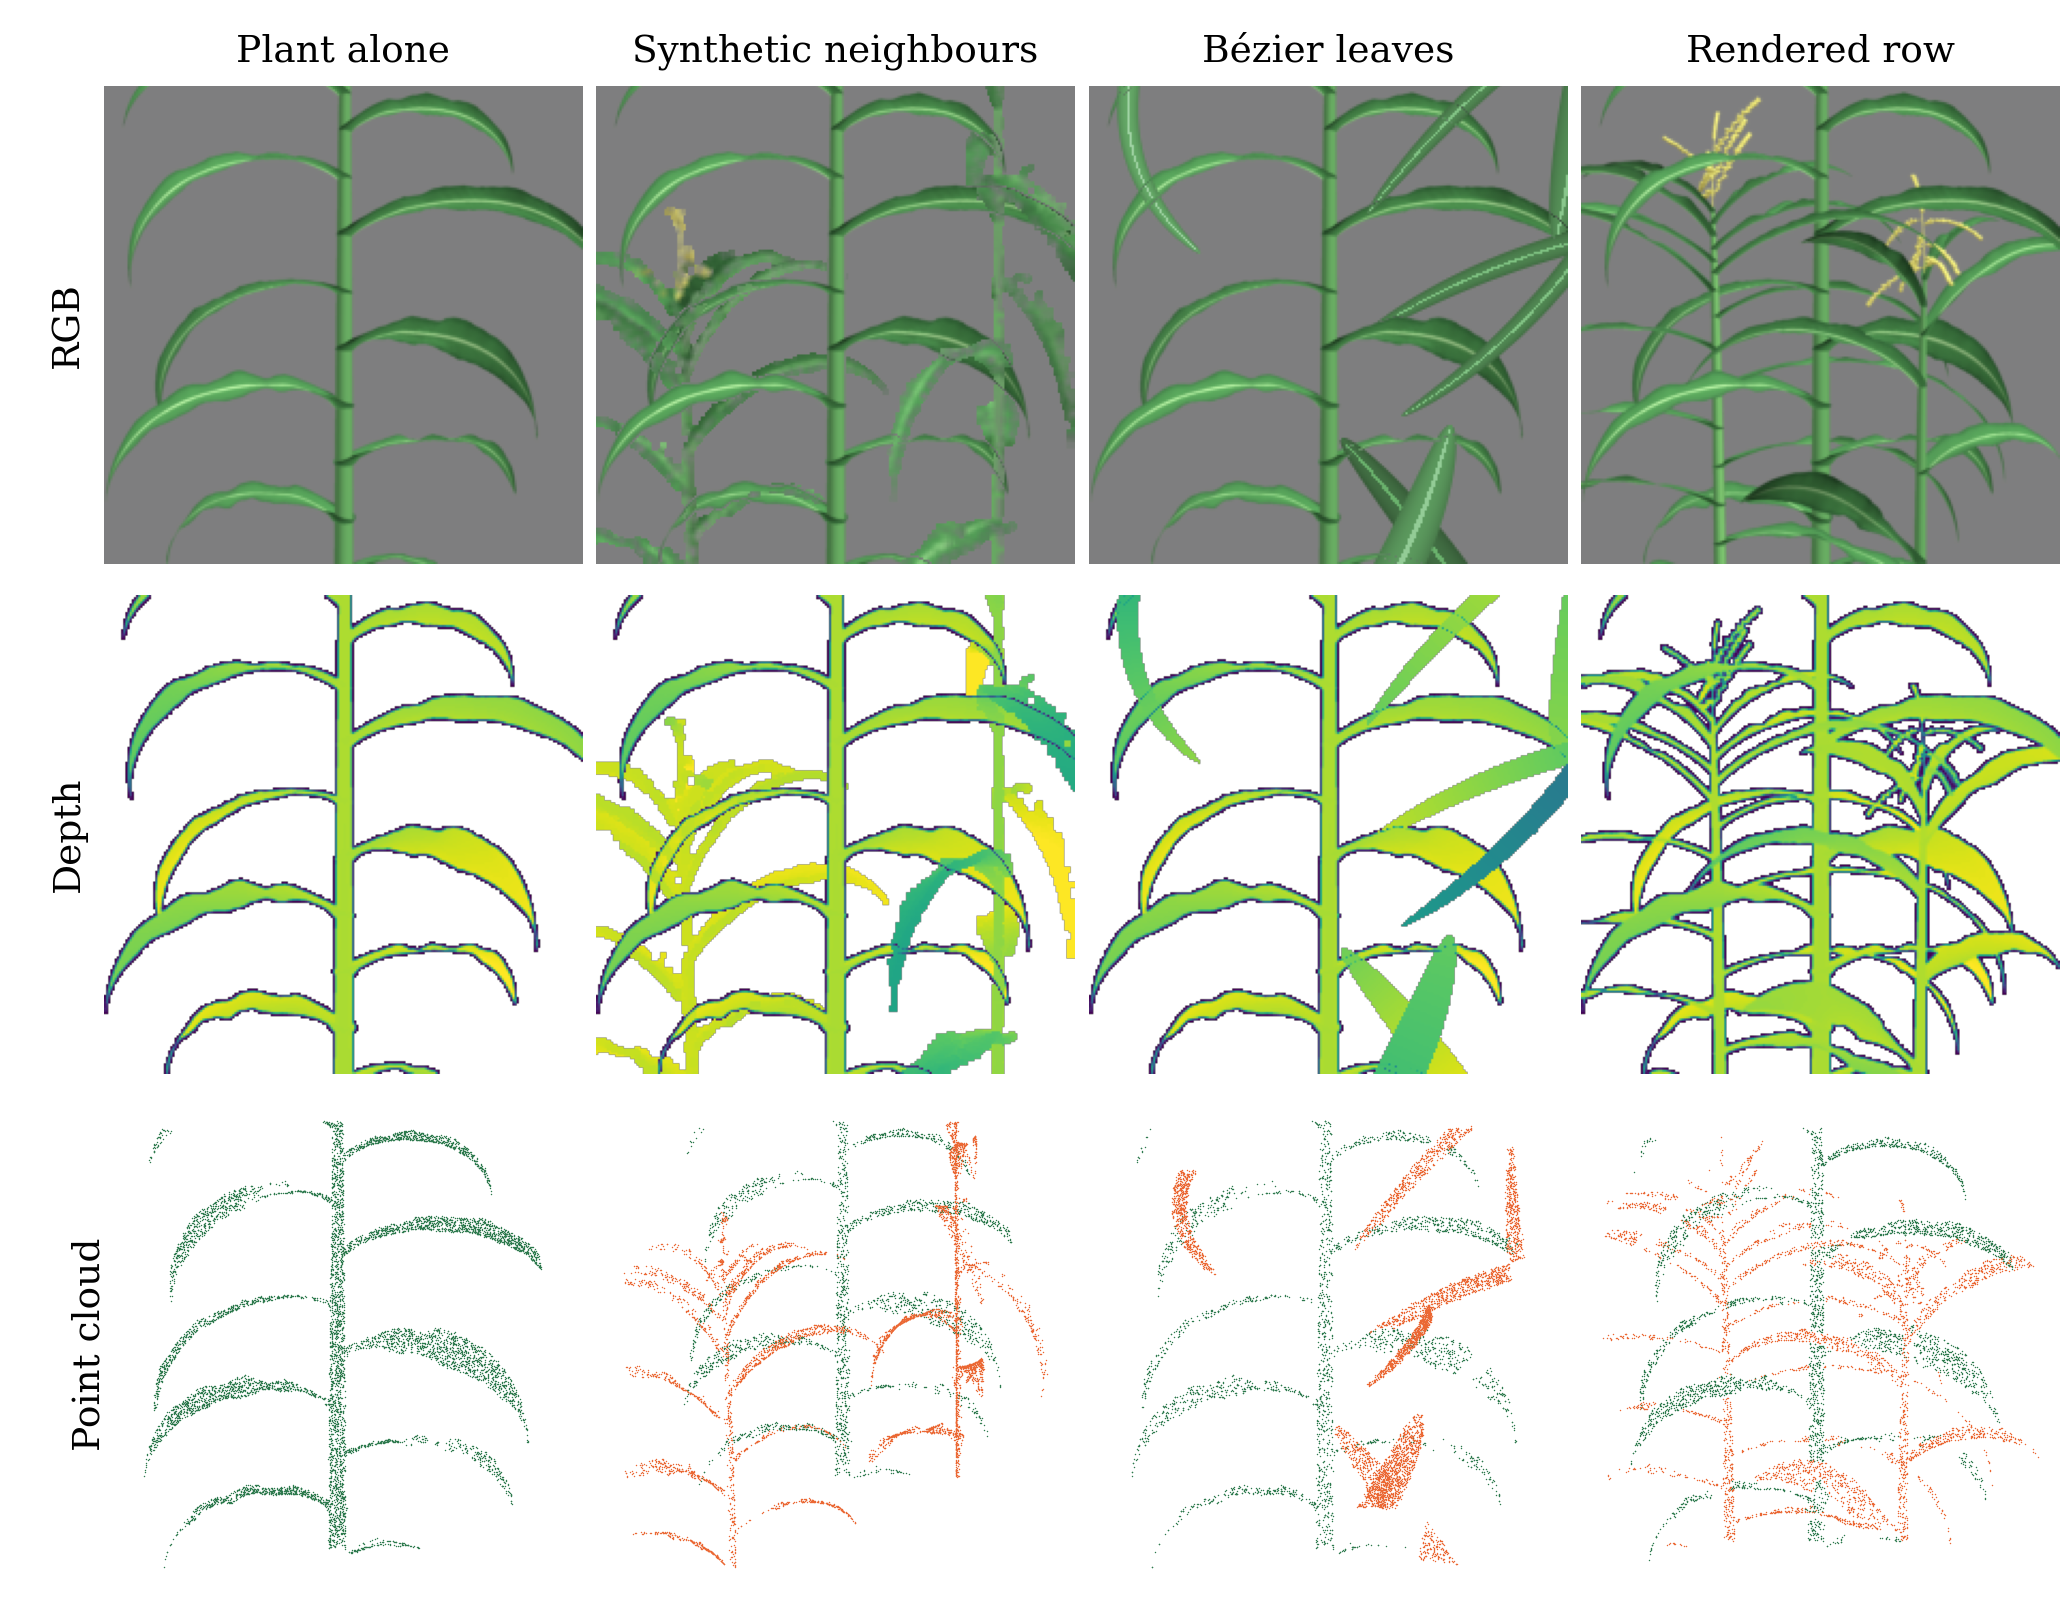
\includegraphics[width=\textwidth]{Figures/fig_sources_maize.png}
  \caption{The four training sources of occlusion, shown for the same maize target plant. Columns: the target
  plant alone; synthetic neighbours (the 3D point clouds of other plants placed beside the target and rendered
  into the image and depth map); B\'ezier leaves (leaf-shaped occluders drawn in the image and depth map and
  lifted to 3D through the camera); and the rendered row. Rows: RGB image, depth map (one colour scale for all
  panels) and point cloud, with target points in green and occluder points in orange.}
  \label{fig:occ_sources}
\end{figure*}

\noindent\textbf{Setup.}
Each rendered maize row shows a target plant with two neighbouring plants 0.15\,m to either side, captured by a
level camera 1\,m away; the reconstruction target is the point cloud of the target plant alone, rendered from
the same camera. All models are EmbodiedMAE-4M (base), start from the same checkpoint pretrained on single
plants, and are trained for 200 epochs with a cosine schedule, learning rate $1.5\times10^{-4}$, a global batch
of 32, 80\% random token masking and the point-cloud loss QAL $+\,0.5\times$Sinkhorn. They differ only in the
occlusion added to the training inputs. \emph{Plant alone}: no occlusion. \emph{Synthetic neighbours}: the
point clouds of two other plants from the batch are placed beside the target in 3D, 0.15--0.35\,m away, and
rendered into the image and depth map with a z-buffer. \emph{B\'ezier leaves}: three to eight leaf-shaped
B\'ezier curves are drawn into the image and depth map, and their visible pixels are lifted to 3D points
through the camera. \emph{Rendered row}: the rendered scene itself. Half of the training samples receive the
occlusion and half show the target plant alone, and the procedural parameters are hidden on half of the steps.

\noindent\textbf{Metrics.}
All models are tested on the rendered rows: 2{,}250 test plants, one fixed view each, with the occluded scene
as input and no procedural parameters. Precision is the fraction of predicted points within 10\,mm of the
target plant, recall the fraction of target points with a prediction within 10\,mm, and F1 their harmonic
mean, averaged over plants.

\begin{table}[t]
  \caption{Effect of the training occlusion on reconstruction of occluded maize plants. All models are tested
  on the rendered occluded rows (2{,}250 test plants, metrics at 10\,mm).}
  \label{tab:abl_occ}
  \centering
  \small
  \begin{tabular}{@{}lccc@{}}
    \toprule
    Training occlusion & F1 $\uparrow$ & Precision $\uparrow$ & Recall $\uparrow$ \\
    \midrule
    Plant alone            & 0.416          & 0.460          & 0.391 \\
    B\'ezier leaves        & 0.552          & 0.639          & 0.507 \\
    Synthetic neighbours   & 0.717          & 0.764          & 0.691 \\
    Rendered row           & \textbf{0.789} & \textbf{0.804} & \textbf{0.782} \\
    \bottomrule
  \end{tabular}
\end{table}

\begin{figure}[t]
  \centering
  \begin{tikzpicture}
    \begin{axis}[abl,
        ybar, bar width=7pt, ymin=0, ymax=1, ytick={0,0.2,0.4,0.6,0.8,1},
        xtick={1,2,3,4}, xmin=0.45, xmax=4.55,
        xticklabels={Plant alone, B\'ezier leaves, Synthetic neighbours, Rendered row},
        x tick label style={font=\footnotesize, align=center, text width=1.55cm},
        ylabel={Score at 10\,mm},
        legend image code/.code={\fill[#1] (0cm,-0.08cm) rectangle (0.22cm,0.12cm);},
      ]
      \addplot[fill=seriesF, draw=white, line width=0.8pt]
        coordinates {(1,0.416) (2,0.552) (3,0.717) (4,0.789)};
      \addplot[fill=seriesP, draw=white, line width=0.8pt] coordinates {(1,0.460) (2,0.639) (3,0.764) (4,0.804)};
      \addplot[fill=seriesR, draw=white, line width=0.8pt] coordinates {(1,0.391) (2,0.507) (3,0.691) (4,0.782)};
      \legend{F1, Precision, Recall}
    \end{axis}
  \end{tikzpicture}
  \caption{Reconstruction of occluded maize plants by training occlusion (data of \cref{tab:abl_occ}). F1, precision and recall rise together as the training occlusion becomes more realistic.}
  \label{fig:abl_occ}
\end{figure}

\noindent\textbf{Results.}
\cref{tab:abl_occ,fig:abl_occ} show that the closer the training occlusion is to the test scenes, the better the
reconstruction. Training on the plant alone gives the lowest F1 (0.416). B\'ezier leaves recover part of the
gap (0.552), and synthetic neighbours, which are real plant geometry placed in 3D, recover most of it (0.717),
but training on the rendered rows remains the best (0.789). Precision and recall improve together at every
step.

%%%%%%%%%%%%%%%%%%%%%%%%%%%%%%%%%%%%%%%%%%%%%%%%%%%%%%%%%%%%%%%%%%%%%%%%%%%%%%%%%%%%%%%%%%%%%%%%%%%%%%%%%%%%%%%%%%%%%%%%%%
\subsection{Mask Ratio During Post-Training}
\label{sec:abl_mask}

We study how much of the input should be masked when the model is trained to reconstruct a plant that is
partly hidden by its neighbours.

\noindent\textbf{Setup.}
We use rendered sorghum rows: each scene shows a target plant with two neighbouring plants 0.15\,m to either
side, captured by a level camera 2.5\,m away. The input is the RGB image, depth map and point cloud of the
scene; the target is the point cloud of the target plant alone, rendered from the same camera. All variants
are EmbodiedMAE-4M (base) and start from the same checkpoint, pretrained on single plants and then trained
for 1{,}000 epochs on the rows at a mask ratio of 0.8. Each variant is fine-tuned for 200 further epochs at
its own mask ratio $m$, with a cosine schedule, learning rate $5\times10^{-5}$, a global batch of 32 and the
point-cloud loss QAL (10\,mm) $+\,0.5\times$Sinkhorn. The mask ratio is the fraction of all input tokens that
are hidden, split across the streams by a Dirichlet draw; $m=0$ keeps every token visible. Half of the
training samples show the occluded scene and half the target plant alone, and the procedural parameters are
hidden on half of the steps. Since every variant starts from a model trained at $m=0.8$, this ablation
measures the mask ratio used for fine-tuning on occluded scenes.

\noindent\textbf{Metrics.}
Each model is tested at the mask ratio it was trained with, on all 2{,}250 test plants (one fixed view each),
with the occluded scene as input and no procedural parameters, using the same metrics at 10\,mm as above.

\begin{table}[t]
  \caption{Effect of the mask ratio on occluded-plant reconstruction (rendered sorghum rows, 2{,}250 test
  plants, metrics at 10\,mm). The mask ratio is the same at training and test time.}
  \label{tab:abl_mask}
  \centering
  \small
  \begin{tabular}{@{}cccc@{}}
    \toprule
    Mask ratio & F1 $\uparrow$ & Precision $\uparrow$ & Recall $\uparrow$ \\
    \midrule
    0.0 & \textbf{0.576} & \textbf{0.606} & \textbf{0.551} \\
    0.2 & 0.555 & 0.590 & 0.526 \\
    0.4 & 0.527 & 0.568 & 0.494 \\
    0.6 & 0.475 & 0.529 & 0.436 \\
    0.8 & 0.379 & 0.464 & 0.325 \\
    \bottomrule
  \end{tabular}
\end{table}

\begin{figure}[t]
  \centering
  \begin{tikzpicture}
    \begin{axis}[abl, width=0.86\columnwidth,
        xmin=-0.04, xmax=0.86, ymin=0.3, ymax=0.65, clip=false,
        xtick={0,0.2,0.4,0.6,0.8}, ytick={0.3,0.4,0.5,0.6},
        xticklabel style={/pgf/number format/.cd, fixed, precision=1, zerofill},
        yticklabel style={/pgf/number format/.cd, fixed, precision=1, zerofill},
        xlabel={Mask ratio (training $=$ test)}, ylabel={Score at 10\,mm},
        legend image code/.code={\draw[#1, line width=1pt] (0cm,0cm) -- (0.3cm,0cm); \fill[#1] (0.15cm,0cm) circle (1.5pt);},
      ]
      \addplot[seriesF, line width=1pt, mark=*, mark size=1.7pt, mark options={fill=seriesF, draw=white, line width=0.4pt}]
        coordinates {(0,0.576) (0.2,0.555) (0.4,0.527) (0.6,0.475) (0.8,0.379)}
        node[pos=1, anchor=west, font=\scriptsize, text=black, xshift=2pt] {F1};
      \addplot[seriesP, line width=1pt, mark=*, mark size=1.7pt, mark options={fill=seriesP, draw=white, line width=0.4pt}]
        coordinates {(0,0.606) (0.2,0.590) (0.4,0.568) (0.6,0.529) (0.8,0.464)}
        node[pos=1, anchor=west, font=\scriptsize, text=black, xshift=2pt] {Precision};
      \addplot[seriesR, line width=1pt, mark=*, mark size=1.7pt, mark options={fill=seriesR, draw=white, line width=0.4pt}]
        coordinates {(0,0.551) (0.2,0.526) (0.4,0.494) (0.6,0.436) (0.8,0.325)}
        node[pos=1, anchor=west, font=\scriptsize, text=black, xshift=2pt] {Recall};
      \legend{F1, Precision, Recall}
    \end{axis}
  \end{tikzpicture}
  \caption{Occluded-plant reconstruction against the mask ratio (data of \cref{tab:abl_mask}). All three
  metrics fall steadily as more of the input is hidden; keeping every token visible is best.}
  \label{fig:abl_mask}
\end{figure}

\noindent\textbf{Results.}
\cref{tab:abl_mask,fig:abl_mask} show that reconstruction improves steadily as the mask ratio decreases: F1
rises from 0.379 at $m=0.8$ to 0.576 with no masking, and precision and recall improve together. Note that every
variant has already been trained with heavy masking (masked pretraining on single plants and 1{,}000 epochs on the
rows at $m=0.8$), so the benefit of masking for learning the representation is already in place. In this
fine-tuning stage, hiding further input tokens only removes evidence about the target plant, and keeping the
whole occluded scene visible works best. This does not imply that training without masking from scratch would be
better, which we did not test.

\subsection{Point-Cloud Loss}
\label{sec:abl_loss}

We compare point-cloud losses for reconstructing single sorghum plants.

\noindent\textbf{Losses.}
Let $\mathcal{P}$ be the predicted point cloud and $\mathcal{T}$ the target cloud, and let
\begin{equation}
  d(x,\mathcal{S})=\min_{s\in\mathcal{S}}\lVert x-s\rVert_2
  =\min_{s\in\mathcal{S}}\sqrt{\textstyle\sum_{k=1}^{3}(x_k-s_k)^2}
  \label{eq:dist}
\end{equation}
be the Euclidean (not squared) distance from a point $x$ to the nearest point of a cloud $\mathcal{S}$. The
quality-aware loss (QAL) weights every nearest-neighbour distance by how far it is from a tolerance $\tau$:
\begin{equation}
  \begin{aligned}
    \mathcal{L}_{\mathrm{QAL}} ={}& \frac{1}{|\mathcal{P}|}\sum_{p\in\mathcal{P}} w\big(d(p,\mathcal{T})\big)\,d(p,\mathcal{T})\\
      &+ \frac{1}{|\mathcal{T}|}\sum_{t\in\mathcal{T}} w\big(d(t,\mathcal{P})\big)\,d(t,\mathcal{P}),
  \end{aligned}
  \label{eq:qal}
\end{equation}
\begin{equation}
  w(d) = \sigma\big(\alpha\,(d-\tau)\big),
  \label{eq:qal_w}
\end{equation}
where $\sigma$ is the logistic function. Points within $\tau$ of the other cloud get a weight below $1/2$
(down to $\sigma(-\alpha\tau)$ at $d=0$), while points far beyond $\tau$ get a weight close to 1, so training
concentrates on the badly placed points, such as missing leaf tips; $\alpha$ sets how sharply the weight switches
at $\tau$. We use
$\alpha=100$ and $\tau=10$\,mm (the clouds are normalised per plant, so $\tau$ is 0.01 of the plant radius, \ie
10\,mm for a plant of median size). \emph{Sinkhorn} is the debiased Sinkhorn divergence $S_\varepsilon(\mathcal{P},\mathcal{T})$ ($p=2$,
blur 0.02) on 1{,}024 sampled points, and \emph{QAL\,+\,Sinkhorn} is
$\mathcal{L}_{\mathrm{QAL}}+\lambda\,S_\varepsilon(\mathcal{P},\mathcal{T})$ with $\lambda=0.5$. Each point-cloud
loss enters the total loss with weight 1.

\noindent\textbf{Single plants.}
Models are trained from scratch on Sorghum\_15K (10{,}500 training plants, one random view per plant per epoch,
each plant rendered alone) for 200 epochs (65.8k steps) with a cosine schedule, learning rate
$1.5\times10^{-4}$, a global batch of 32 and 80\% token masking, and differ only in the point-cloud loss. They
are tested on all 2{,}250 test plants with the plant alone as input.

\noindent\textbf{Metrics.}
Precision is the fraction of predicted points within a threshold of the target plant, recall the fraction of
target points with a prediction within the threshold, and F1 their harmonic mean, averaged over plants. We write
F1@$x$, Prec.@$x$ and Rec.@$x$ for a threshold of $x$\,mm.

\begin{table}[t]
  \caption{Point-cloud losses on single plants (sorghum, trained from scratch, 2{,}250 test plants).}
  \label{tab:loss_single}
  \centering
  \small
  \setlength{\tabcolsep}{3pt}
  \begin{tabular}{@{}lcccc@{}}
    \toprule
    Loss & F1@5 & F1@10 & Prec.@10 & Rec.@10 \\
    \midrule
    QAL              & 0.057          & 0.224          & \textbf{0.561} & 0.144 \\
    Sinkhorn         & 0.045          & 0.168          & 0.142          & \textbf{0.206} \\
    QAL\,+\,Sinkhorn & \textbf{0.083} & \textbf{0.259} & 0.422          & 0.189 \\
    \bottomrule
  \end{tabular}
\end{table}

\begin{table}[t]
  \caption{QAL parameter screen (sorghum single plants, epoch 300, 225 validation views). Here @10 is a
  threshold of 0.01 of the plant radius ($\approx$10\,mm). The row $\tau=10$\,mm, $\alpha=100$ is taken from a longer run
  (300k-step schedule) at the same epoch, so its learning rate had not yet decayed.}
  \label{tab:qal_params}
  \centering
  \small
  \begin{tabular}{@{}ccccc@{}}
    \toprule
    $\tau$ & $\alpha$ & F1@10 & Prec.@10 & Rec.@10 \\
    \midrule
    5\,mm  & 100 & 0.155 & 0.398 & 0.107 \\
    10\,mm & 100 & 0.154 & 0.398 & 0.107 \\
    20\,mm & 100 & 0.139 & 0.384 & 0.097 \\
    10\,mm & 30  & 0.146 & 0.403 & 0.101 \\
    10\,mm & 300 & \textbf{0.164} & \textbf{0.406} & \textbf{0.115} \\
    \bottomrule
  \end{tabular}
\end{table}

\noindent\textbf{Results.}
Neither kind of loss is sufficient on its own (\cref{tab:loss_single}). QAL, which matches every point to its
nearest neighbour, places points precisely but leaves much of the plant uncovered (Rec.@10 0.144), while the
Sinkhorn divergence covers more of the plant but places points poorly (Prec.@10 0.142). Adding a Sinkhorn term to
QAL gives the best F1 at both thresholds: it improves F1@5 over QAL by 0.026 and F1@10 by 0.035 (better on 82\% of
plants), mainly by raising recall at a moderate cost in precision.

\noindent\textbf{QAL parameters.}
We screened the tolerance $\tau$ and the sharpness $\alpha$ of \cref{eq:qal_w} in a shorter setting: sorghum
single plants, 3{,}000 training plants, trained from scratch with a 30k-step (320-epoch) cosine schedule, 75\% token
masking and synthetic leaf occluders with sensor noise added to the training inputs, using QAL alone as the
point-cloud loss. Each setting was trained once and is scored at epoch 300 on 225 clean validation views
(\cref{tab:qal_params}).

A sharper weighting ($\alpha=300$) gives the highest F1, precision and recall, and a tolerance of 20\,mm is the
weakest; a tolerance of 5 or 10\,mm performs the same. The differences are small (at most 0.025 F1), come from a
single seed and a short schedule, and should be read as a screen rather than a final ranking.

\subsection{Mixed Masking}
\label{sec:abl_mixed}

When the training input is occluded, the masking can target the occluder. \emph{Structured} masking hides the
tokens that show an occluder first (an image patch that is at least 30\% occluder pixels, or a point-cloud token
whose centre is an occluder point) and fills the rest of the masking budget at random. \emph{Mixed} masking flips
one coin per occluded training scene: with probability 0.5 the scene is masked structured, otherwise uniformly at
random (\cref{fig:mixed}). We compare mixed masking with uniform \emph{random} masking. Validation and test always
use random masking.

\begin{figure*}[t]
  \centering
  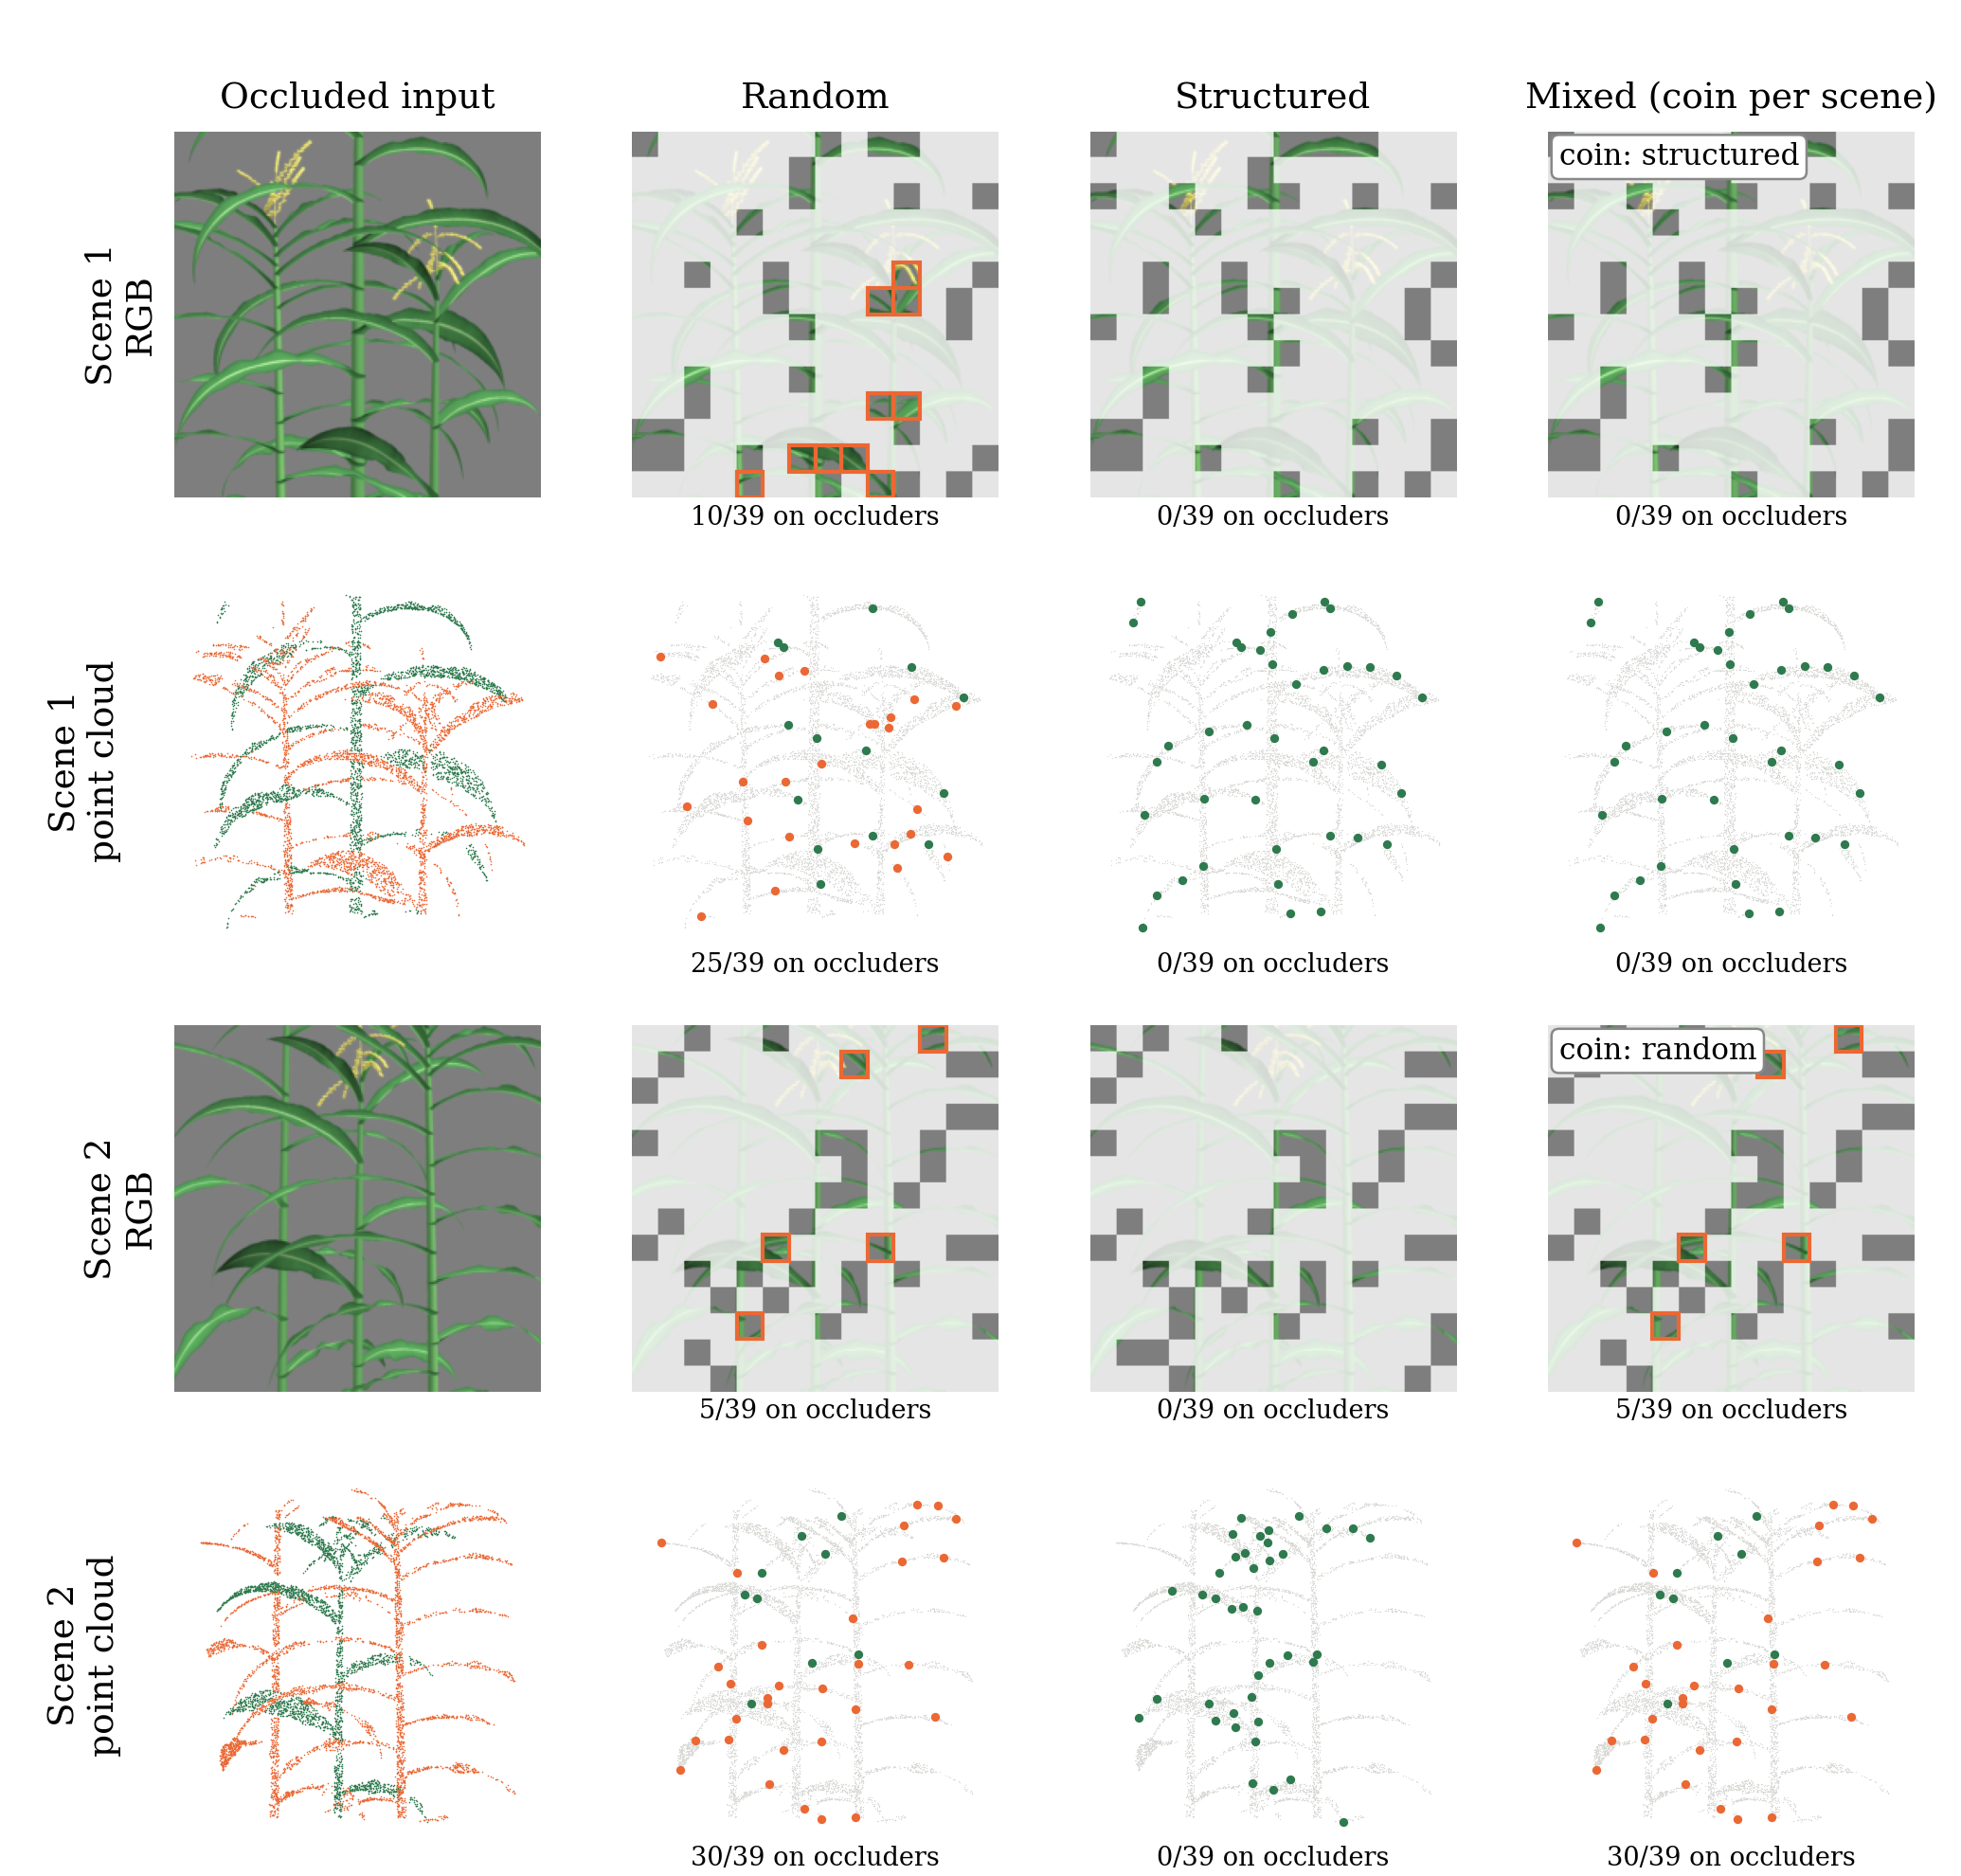
\includegraphics[width=0.85\textwidth]{Figures/fig_mixed_masking.png}
  \caption{Mixed masking with one coin per scene, on two occluded maize scenes from the rendered rows. Columns: the
  occluded input (point cloud: target plant in green, occluders in orange); random masking; structured masking, which
  masks the occluder tokens first; and mixed masking, where a coin per training scene selects structured masking
  (scene 1) or random masking (scene 2). For illustration, every masked panel keeps the same 20\% of the tokens of
  each modality visible, drawn with the same random numbers, so only the policy differs. Images: masked patches are
  faded, visible patches are in full colour (the render background is grey), and visible occluder patches are
  outlined in orange. Point clouds: dots mark the centres of the visible point
  tokens (green: target, orange: occluder). Below each panel: visible tokens that lie on occluders, out of 39.}
  \label{fig:mixed}
\end{figure*}

\noindent\textbf{Setup.}
All models are EmbodiedMAE-4M (base) trained for 200 epochs with a cosine schedule, a global batch of 32, 80\% token
masking and the point-cloud loss QAL\,$+\,0.5\times$Sinkhorn; half of the training samples are
occluded. The two models of each pair differ only in the masking. \emph{Synthetic scenes}: the point clouds of two
other plants from the batch are placed beside the target plant in 3D and rendered into its image and depth map;
these models are trained from scratch and receive the target's procedural parameters as input in training and
test. \emph{Rendered rows}: the target plant is rendered with its two neighbouring plants 0.15\,m to either side,
and no procedural parameters are given at test. The maize rendered-row models are trained from scratch; the
sorghum ones are fine-tuned from a model already trained for 1{,}000 epochs on the rendered rows with random
masking. In the maize pair, the mixed model was trained with 8 samples per GPU on 4 GPUs and the random model with
16 per GPU on 2 GPUs (the same global batch).

\noindent\textbf{Metrics.}
Every model is tested on all 2{,}250 test plants, one view each, with the occluded input. F1@$x$ is the harmonic
mean of precision (predicted points within $x$\,mm of the target plant) and recall (target points with a
prediction within $x$\,mm), averaged over plants.

\begin{table*}[t]
  \caption{Mixed masking (one coin per scene) against random masking on occluded test input (2{,}250 test plants).
  $\Delta$ is mixed minus random in F1@10. The better F1@10 of each pair is in bold.}
  \label{tab:mixed_scene}
  \centering
  \small
  \begin{tabular}{@{}lllccccc@{}}
    \toprule
    & & & \multicolumn{2}{c}{Random} & \multicolumn{2}{c}{Mixed} & \\
    \cmidrule(lr){4-5}\cmidrule(lr){6-7}
    Training occlusion & Tested on & Species & F1@5 & F1@10 & F1@5 & F1@10 & $\Delta$F1@10 \\
    \midrule
    Synthetic scenes & synthetic scenes & maize   & 0.160 & 0.439 & 0.190 & \textbf{0.487} & $+0.048$ \\
    Synthetic scenes & synthetic scenes & sorghum & 0.112 & 0.310 & 0.119 & \textbf{0.323} & $+0.013$ \\
    \midrule
    Rendered rows & rendered rows & maize   & 0.525 & \textbf{0.775} & 0.522 & 0.771 & $-0.003$ \\
    Rendered rows & rendered rows & sorghum & 0.133 & \textbf{0.377} & 0.133 & 0.373 & $-0.004$ \\
    \bottomrule
  \end{tabular}
\end{table*}

\noindent\textbf{Results.}
Mixed masking helps only on the synthetic scenes: F1@10 rises by 0.048 in maize and by 0.013 in sorghum
(\cref{tab:mixed_scene}). On the rendered rows it gives no gain in either species ($-0.003$ in maize and $-0.004$
in sorghum).

% =========================================================================
\section{Real-Row Fine-Tuning Gallery (E10)}
\label{sec:supp-e10}

Figures~\ref{fig:supp-e10-maize} and~\ref{fig:supp-e10-sorghum} extend the real-row results of Sec.~\ref{sec:res-field} to 20 more held-out plants, none of which the real-row fine-tune saw. Each tile shows the image the model reads, the true center plant as the camera sees it, and the center plant written before fine-tuning on real plants (the row fine-tune, trained on synthetic rows only) and after it (the real-row fine-tune, trained on the other 75\% of the real plants). All three streams are in. Chamfer is in $10^{-4}$\,m$^2$. The maize tiles are chosen across the range of the fine-tuned model's results, at the 10th, 30th, 50th, 70th, 90th and 98th percentile of its Chamfer in each row layout, so the bottom tiles are among its worst cases. Every tile improves: the maize Chamfer goes from 20--195 before fine-tuning to 6--52 after, and the predicted height moves from about 1.0\,m for every plant to within a few centimeters of the true height (for example 1.52 against 1.52\,m and 1.88 against 1.85\,m). The worst maize tile after fine-tuning (Chamfer 52) also has the largest height error in the gallery, 1.23 against 1.30\,m. The sorghum tiles cover all eight held-out plants. Their Chamfer goes from 661--2{,}781 before to 52--122 after; the fine-tuned model recovers the stalk over the full height of plants 2.8--4.9\,m tall, but few of the leaves.

\begin{figure*}[p]
  \centering
  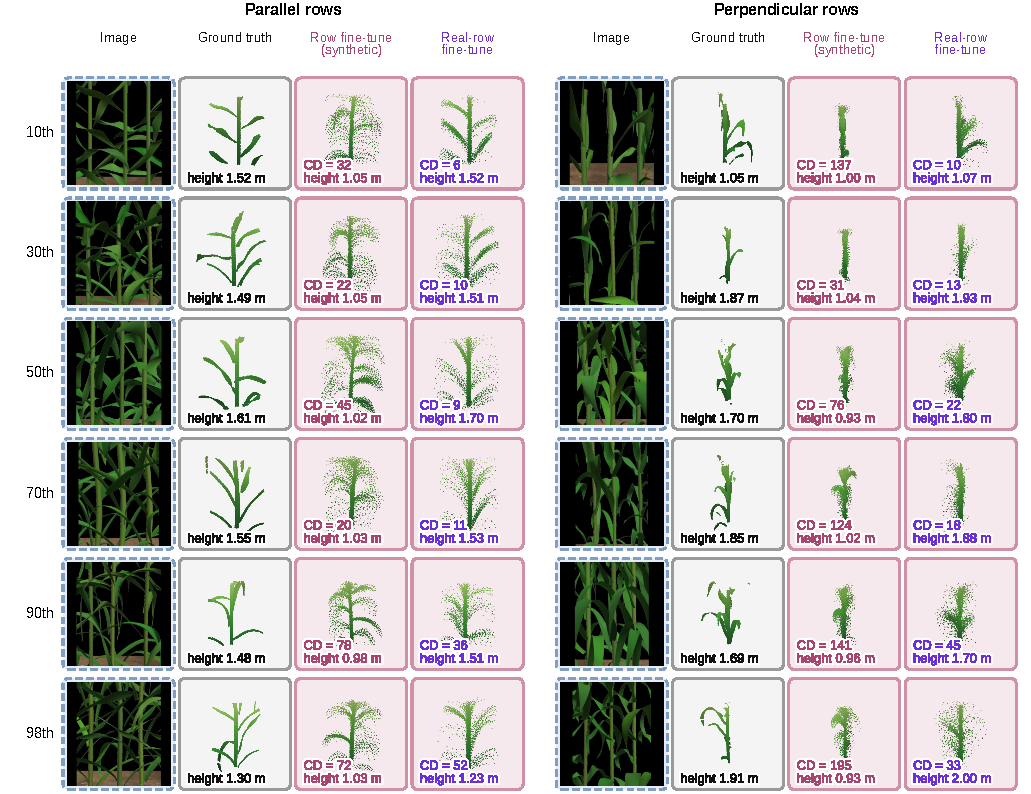
\includegraphics[width=\textwidth]{Figures/fig_e10_gallery_maize_ugg.pdf}
  \caption{\textbf{Real maize rows, held-out plants (E10).} Left: parallel rows; right: perpendicular rows; from top to bottom the 10th, 30th, 50th, 70th, 90th and 98th percentile of the real-row fine-tune's Chamfer. Columns: the image the model reads, the ground-truth center plant with its height, and the center plant from the row fine-tune (synthetic rows) and from the real-row fine-tune (75\% of the real plants), each with CD, its Chamfer distance to the ground truth ($10^{-4}$\,m$^2$), and its height.}
  \label{fig:supp-e10-maize}
\end{figure*}

\begin{figure*}[t]
  \centering
  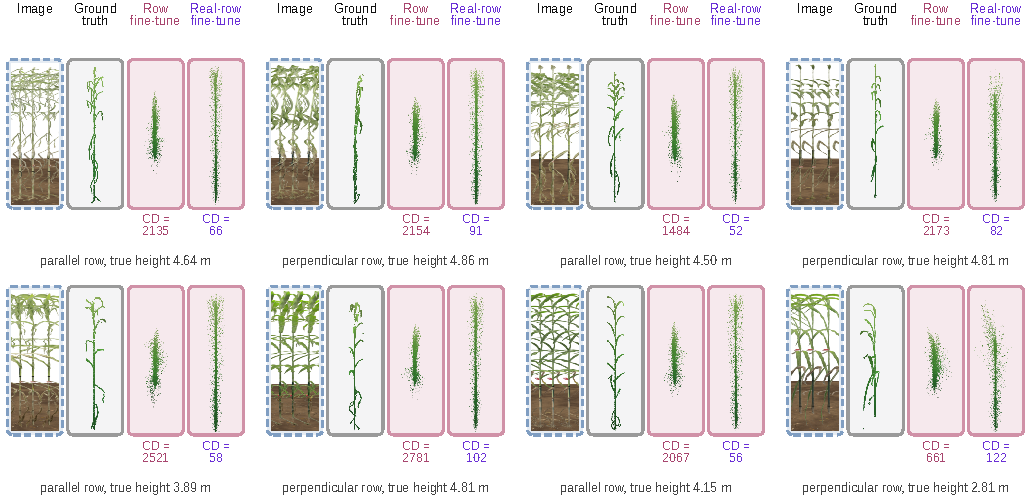
\includegraphics[width=\textwidth]{Figures/fig_e10_gallery_sorghum_ugg.pdf}
  \caption{\textbf{Real sorghum rows, all eight held-out plants (E10).} The middle camera stop of each plant, layouts alternating; columns as in Fig.~\ref{fig:supp-e10-maize}. The image is the camera photograph, a tall strip framed to the whole plant. Sorghum has no height truth comparable to the recipe, so each prediction gives only CD, its Chamfer distance to the ground truth ($10^{-4}$\,m$^2$); the true plant height is given under each plant.}
  \label{fig:supp-e10-sorghum}
\end{figure*}

% =========================================================================
\section{Row Occlusion Gallery (Regime III)}
\label{sec:supp-rows}

Figures~\ref{fig:supp-rows-sorghum} and~\ref{fig:supp-rows-maize} extend Fig.~\ref{fig:rowsex} to ten more held-out test plants per species. Unlike Fig.~\ref{fig:rowsex}, these plants are not selected for clarity: they sit at the 5th, 15th, \dots, 95th percentile of the row-trained model's Chamfer distance (mean of the two yaws) over the 2{,}250 test plants of each species, so the lower rows show its harder cases.

\begin{figure*}[p]
  \centering
  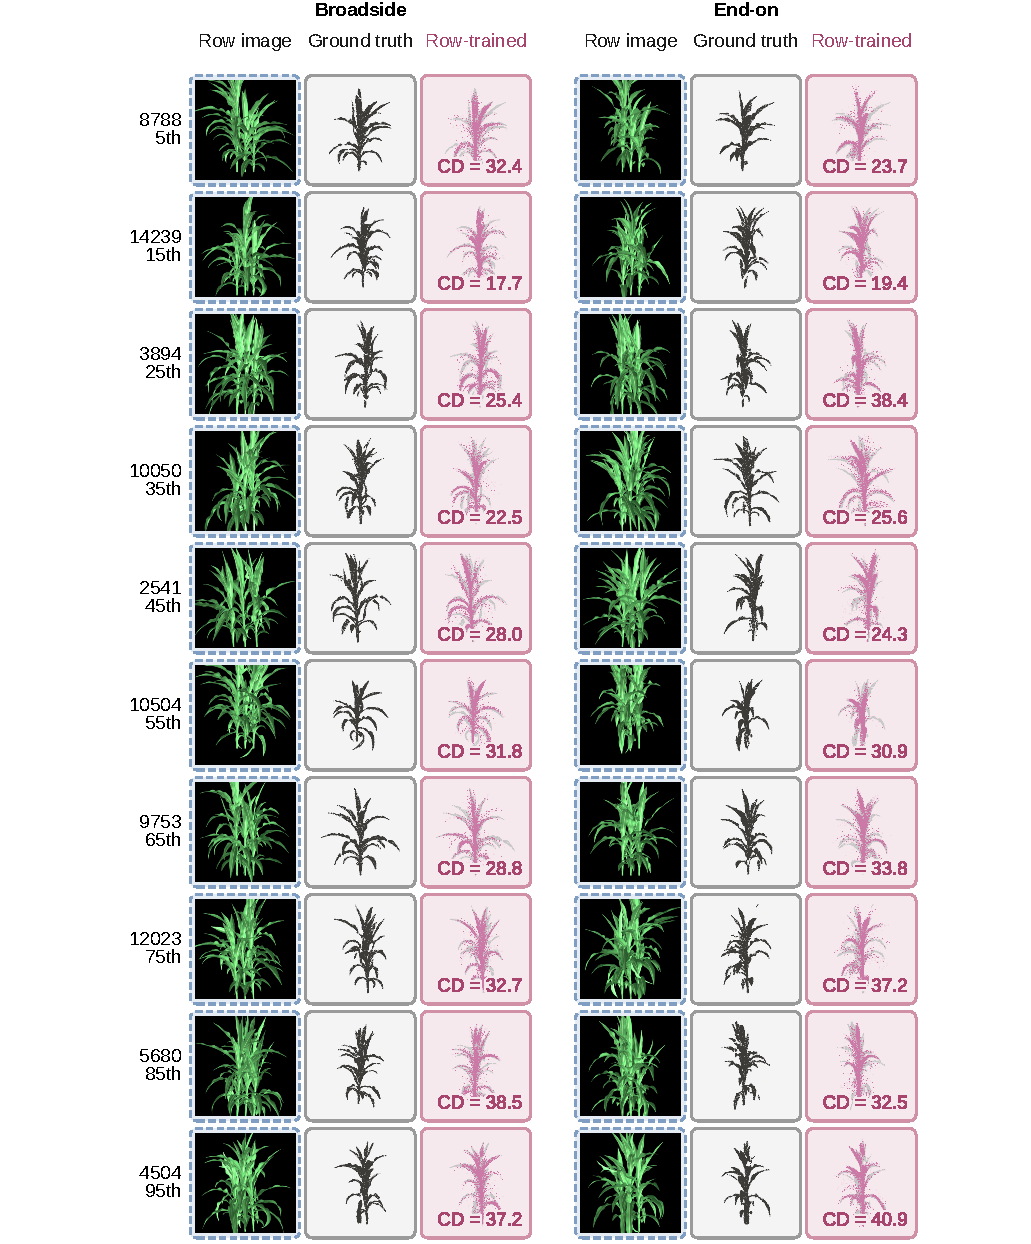
\includegraphics[width=\linewidth]{Figures/fig_rows_more_sorghum_ugg.pdf}
  \caption{\textbf{Sorghum rows, ten held-out test plants at evenly spaced percentiles of the row-trained error.} Each row gives the plant number and its percentile; broadside (left) and end-on (right); columns as in Fig.~\ref{fig:rowsex}: row image, ground truth, row-trained model (pink) over the ground truth in grey, CD = its Chamfer distance to the ground truth in $10^{-4}\,\mathrm{m}^2$.}
  \label{fig:supp-rows-sorghum}
\end{figure*}

\begin{figure*}[p]
  \centering
  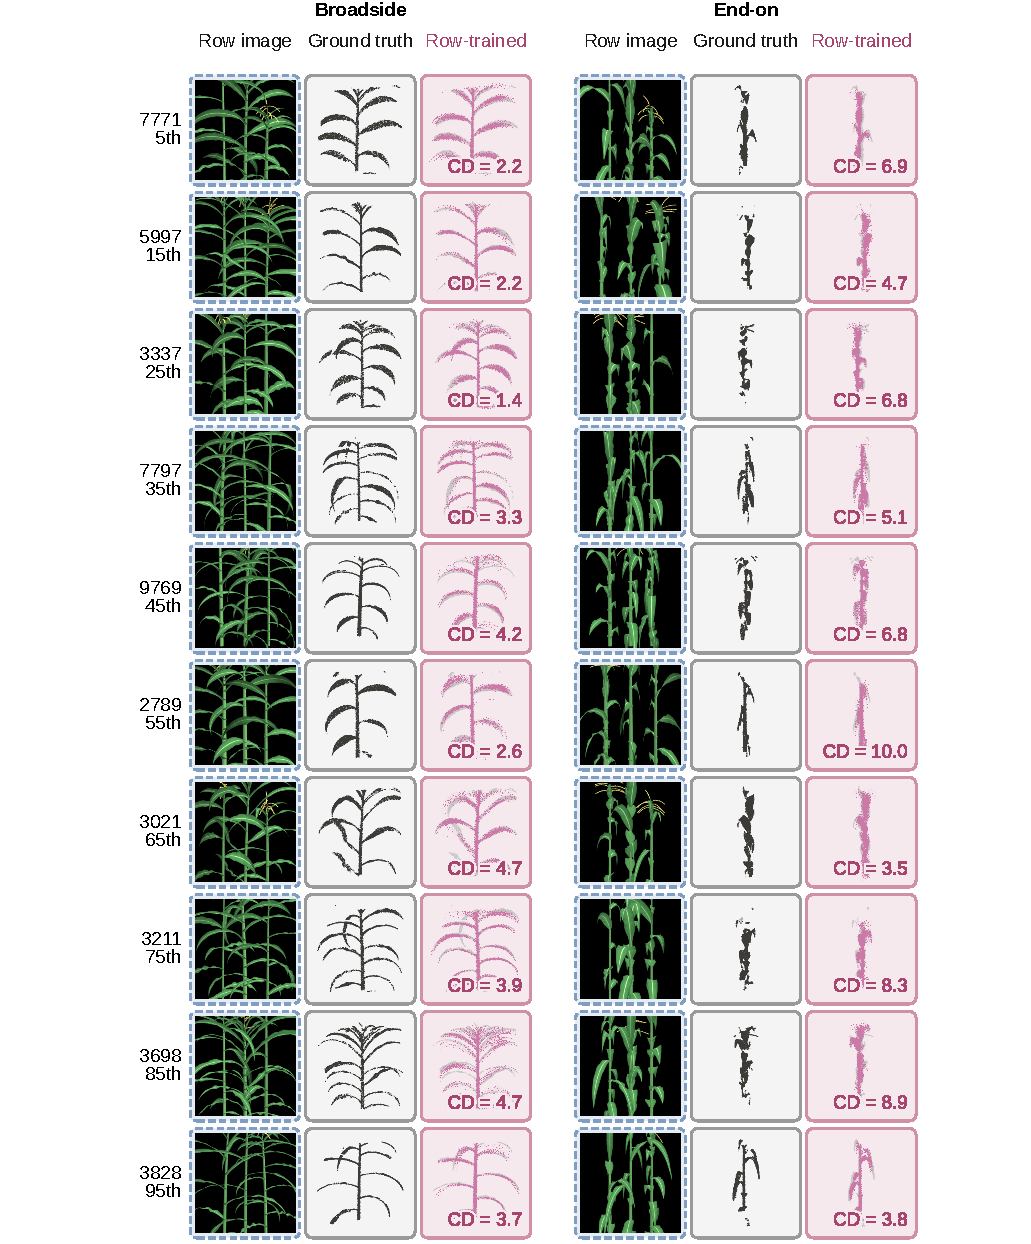
\includegraphics[width=\linewidth]{Figures/fig_rows_more_maize_ugg.pdf}
  \caption{\textbf{Maize rows, ten held-out test plants at evenly spaced percentiles of the row-trained error.} Each row gives the plant number and its percentile; broadside (left) and end-on (right); columns as in Fig.~\ref{fig:rowsex}: row image, ground truth, row-trained model (pink) over the ground truth in grey, CD = its Chamfer distance to the ground truth in $10^{-4}\,\mathrm{m}^2$.}
  \label{fig:supp-rows-maize}
\end{figure*}

\clearpage   % print the two row galleries right after their section

\section{Dataset Generation Details}
\label{app:data}

\dataset{} contains four synthetic sets: isolated single-plant captures of
maize and sorghum, alongside simulated \emph{row scenes} captured by a
level ground rover. All images are rendered at $1024 \times 1024$
resolution with a $40^\circ$ vertical field of view
($f_x = f_y = 512 / \tan 20^\circ = 1406.7$\,px, principal point at image
center) in OpenGL camera coordinates ($+y$ up, camera looking along $-z$).

\subsection{Procedural crop generation}
\noindent\textbf{Maize procedural generation.} Each plant $i$ of $15{,}000$ is
generated from seed $i$ using a procedural maize generator. Morphological
traits are sampled from Gaussian distributions: plant height
$0.832 \pm 0.104$\,m, leaf count $12.35 \pm 2.57$, base leaf length
$0.448 \pm 0.057$\,m, base leaf width $0.066 \pm 0.010$\,m, and base leaf
insertion angle $43.98^\circ \pm 10.13^\circ$. Attributes are coupled
through four latent traits (vigor, slenderness, posture, texture) with
correlation strength 0.735, canopy position curves (bottom, middle, top),
and per-leaf spatial jitter (scale 0.687). Plant heights span 0.62--1.44\,m
(median 1.01\,m). Parameter records store plant height, leaf count, and
per-leaf stem insertion height, length, width, azimuth, insertion angle,
and droopiness. Per-leaf curvature is generated by constructing midrib
B-splines and integrating bending curvature along leaf blades using
10-node Gauss--Legendre quadrature.

\noindent\textbf{Sorghum procedural generation.} Each plant $i$ of $15{,}000$ is
generated from seed $i$ using the EvoEngine sorghum generator. Heading
angle is sampled uniformly in $[0^\circ, 360^\circ)$, stem tilt
$0^\circ \pm 1.5^\circ$, leaf count $20 \pm 2$ (clamped to $[2, 128]$), and
internode spacing $0.04 \pm 0.03$\,m. Stem length is evaluated as
$\text{internode} \times n_{\text{leaves}} / (1 - s_0)$, where $s_0$
represents the first leaf insertion point. Continuous curves over relative
height $t \in [0, 1]$ determine leaf insertion height, blade length, width,
roll ($\text{roll}_k = (k \bmod 2) \cdot 180^\circ + \text{roll}(t)$),
branching angle, and bending curvature. Sorghum plants contain 4--35 leaves
(mean 19.5) on stems ranging from 0.19\,m to 1.74\,m.

\subsection{Dataset partitioning}
Both species are partitioned into 10{,}500 training, 2{,}250 validation,
and 2{,}250 test plants (70\% / 15\% / 15\%).
\begin{itemize}
\item  \textbf{Maize partitioning}: 19 scalar morphological features are
  robustly standardized using median absolute deviation
  ($z = (x - \mathrm{median}) / (1.4826 \cdot \mathrm{MAD})$). Each plant
  is scored by Mahalanobis distance
  $\sqrt{z^\top (\Sigma + 10^{-6}I)^{+} z}$. The most extreme plants are
  dealt alternately to test and validation splits to form an extreme tail
  split (train scores 1.56--4.60, validation 4.60--23.3, test 4.60--32.2). \item  \textbf{Sorghum partitioning}: Plants are partitioned based on
  Mahalanobis distance across six core traits: leaf count, stem length,
  mean leaf length, maximum leaf length, mean leaf roll, and leaf roll
  standard deviation. Sampling probabilities scale continuously with
  extremeness rank, rising from 0.3\% in the least extreme 5\% of plants to
  70\% in the most extreme 5\% (median rank 0.75 on validation and test,
  0.37 on train). The rule is: each plant's extremeness is its Mahalanobis
  distance from the centroid of the six standardized traits, ranked to a
  percentile $r\in[0,1]$; a pool of 30\,\% of the plants is drawn without
  replacement with probability proportional to $(r+0.02)^2$ (seed 42), shuffled,
  and split equally into test and validation, and the rest is the training split.
  Re-running this procedure (\texttt{data\_split/make\_split.py}) reproduces
  the released assignment for all 15{,}000 plants.
\end{itemize}
Figure~\ref{fig:dataset_stats} shows the resulting split densities, the
trait structure of the two generators and the occlusion the row scenes
produce.

\begin{figure*}[t]
  \centering
  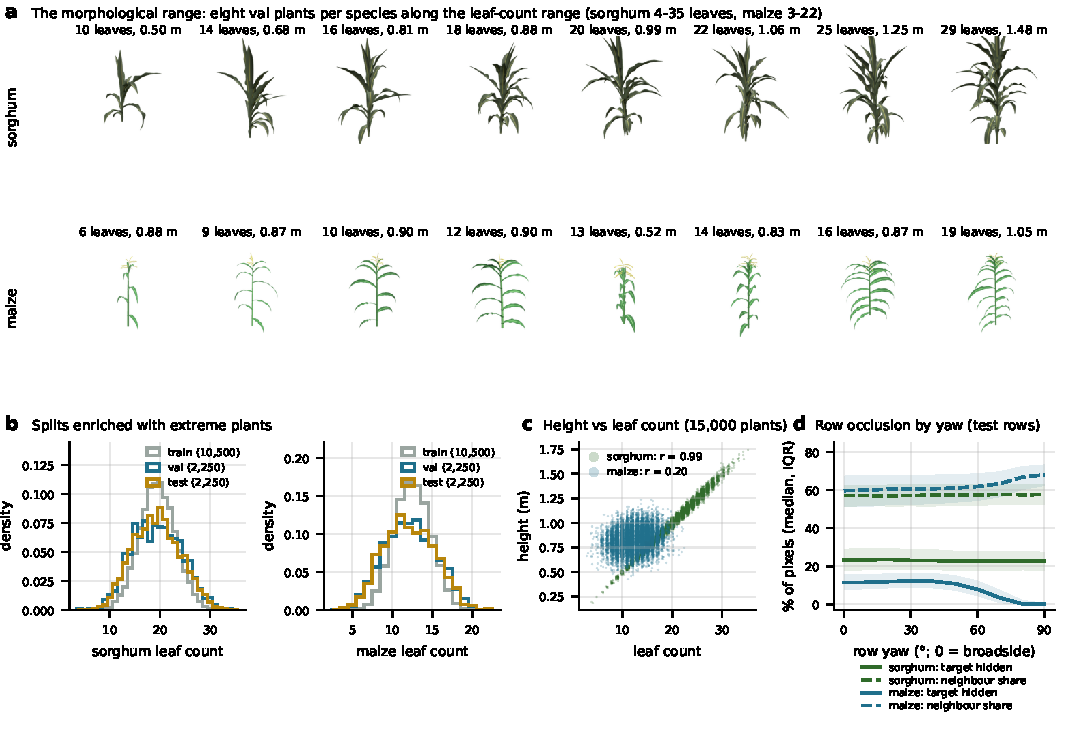
\includegraphics[width=\linewidth]{Figures/fig_dataset_stats.pdf}
  \caption{\textbf{What \dataset{} spans.} (a) Eight validation plants per
  species along the leaf-count range, photographed near the horizon. (b)
  Leaf-count densities per split: validation and test are enriched with
  extreme plants. (c) Plant height against leaf count for all 15{,}000 plants
  per species: the sorghum generator ties the two ($r = 0.99$), in maize they
  are nearly independent ($r = 0.20$). (d) Row occlusion by yaw on the test
  rows: the share of the target's pixels hidden behind a neighbor (solid) and
  the share of plant pixels that belong to neighbors (dashed), median and
  interquartile range over plants.}
  \label{fig:dataset_stats}
\end{figure*}

\subsection{Isolated-plant sensor rendering}
Off-screen rendering is executed via \texttt{pyrender}. Cameras target the
plant bounding-box center $\mathbf{c}$ with world up $(0,1,0)$. Lighting
consists of 0.15 ambient illumination plus three white directional lights
directed at $\mathbf{c}$ from $(1,1,1)$, $(-1,0.5,-0.5)$, and $(0,1,0)$
(intensities 4.0, 2.0, 1.5) against a neutral gray background (0.5). Depth
$z \in [n, f]$ is packed losslessly into 32-bit RGBA PNG files:
\begin{equation}
  v = \left\lfloor \mathrm{clip}\left(\frac{z-n}{f-n}, 0, 1\right) (2^{32}-1) \right\rfloor.
\end{equation}
Pixels $(u,v)$ with depth $z > 0$ back-project to 3D camera coordinates:
\begin{equation}
  \mathbf{p}_{\mathrm{cam}} = \left( \frac{u - c_x}{f_x} z,\; -\frac{v - c_y}{f_y} z,\; -z \right).
  \label{eq:supp-backproject}
\end{equation}

\noindent\textbf{Maize captures.} Ten camera directions per plant are sampled
uniformly on the sphere (normalized Gaussian vectors), at a
distance fitted to the plant: with $r$ half the bounding-box diagonal,
\begin{equation}
  \mathrm{dist} = \frac{1.05\,r}{\sin 20^\circ},\quad
  \begin{aligned}
    n &= \max(0.001,\ \mathrm{dist} - 1.5\,r),\\
    f &= \mathrm{dist} + 1.5\,r.
  \end{aligned}
  \label{eq:supp-maizecam}
\end{equation}
A fourth directional light (1.5) is
mounted to the camera. Outputs include RGB images, RGBA images with cleared
backgrounds, depth maps, camera poses, parameter records, and
8{,}192-point clouds back-projected from view depth maps.

\noindent\textbf{Maize leaf curvature.} The parameter record's per-leaf
curvature is computed on the midrib B-spline rebuilt from the leaf's length,
insertion angle, droopiness and spline point count (cubic, clamped, target
elevation $\mathrm{angle} + \mathrm{droop}\cdot t^2$): over blade arc length
$s \in [0.22, 1]$,
\begin{equation}
  \theta = \int_{0.22}^{1} \lvert \kappa(s) \rvert \, ds,
  \qquad \bar\kappa = \theta / S,
  \label{eq:supp-curvature}
\end{equation}
with $\theta$ the total bend angle, $S$ the blade length and
$\bar\kappa$ the mean curvature, all integrated by 10-node
Gauss--Legendre quadrature.

\noindent\textbf{Sorghum captures.} Ten camera directions form a fixed Fibonacci
sphere rig at 2.5\,m distance ($y_i = 1 - 2(i+0.5)/10$,
$\phi_i = i(\sqrt5-1)\pi + \epsilon_i$ with a small fixed jitter
$\epsilon_i$; elevation angles $-64^\circ$ to $+64^\circ$, five above and
five below the horizon). Outputs include RGB images, depth maps, camera
poses, parameter records, and complete occlusion-free 8{,}192-point clouds
expressed in the camera frame.

\subsection{Simulated crop row rendering}
\noindent\textbf{Row composition.} Within a split, row $i$ places target main
plant $L_i$ between right neighbor $L_{i+1}$ and left neighbor $L_{i+2}$ at
stem spacing $d = 0.15$\,m along the $x$-axis. Rows are rendered across ten
orientation angles $\theta \in \{0^\circ, 10^\circ, \dots, 90^\circ\}$ with
random neighbor offsets $\delta \sim U(-15^\circ, 15^\circ)$. Sorghum
neighbors are rotated so their stem axes run parallel to the main stem%
: each neighbor is turned about its stem base by the smallest
rotation that makes its stem direction (the principal SVD axis of its stem
vertices), after its own yaw, parallel to the main plant's stem direction
after the main yaw. The main plant is never tilted, and maize is not
tilted.

\noindent\textbf{Physical contact solver.} Inter-plant leaf collisions are
resolved using an articulated contact solver. Leaf blades are modeled as
chains of 8\,cm segments connected by joints that bend along circular arcs,
up/down and sideways. Stems, sheaths (within 2.5\,cm of stem axes), and
maize tassels remain rigid. Upon collision, joints rotate by the minimum
clearing angle required to eliminate triangle--triangle intersection. Neighbors bend first; main plant leaves bend only when neighbors reach
rotation limits (Tab.~\ref{tab:supp-stages}). When no valid layout exists
under default limits, limits loosen in stages, and stem spacing widens in
5\,cm steps (refined to 1\,cm); the maximum spacing used in maize is
0.33\,m.

\begin{table}[h]
  \caption{\textbf{Physical contact solver staged bending thresholds.} Joint
rotation limits applied across optimization stages to resolve inter-plant
row leaf collisions.}
\label{tab:supp-stages}\label{tab:supp-solver_limits}
\centering\scriptsize
\setlength{\tabcolsep}{3pt}
\begin{tabular}{lcccc}
\toprule
Stage & Collar side & Blade side & Up/down & Total turn \\
\midrule
Stage 0 (default) & $30^\circ$ & $10^\circ$ & $45^\circ$ & $90^\circ$ \\
Stage 1 (medium)  & $60^\circ$ & $10^\circ$ & $60^\circ$ & $120^\circ$ \\
Stage 2 (loose)   & $90^\circ$ & $30^\circ$ & $70^\circ$ & $180^\circ$ \\
\bottomrule
\end{tabular}

\end{table}

\noindent\textbf{Contact detection (\Meets).} Whether a leaf \emph{meets}
another plant is decided in two steps. (1)~\emph{Grid screen}: each plant
marks a 1\,cm occupancy grid at surface samples that cover every surface
point to within $\varepsilon_O = 2.8$\,mm, and the marked cells are grown by
one cell in every direction; the tested leaf is sampled so that every point
of it lies within $\varepsilon_M = 6.8$\,mm of a sample. Where two surfaces
cross, some tested sample and some marked sample lie within
$\varepsilon_M + \varepsilon_O < 1$\,cm of each other, so the tested sample
falls in a grown cell: no tested sample in another plant's grown cells means
no crossing. (2)~\emph{Exact test}: each triangle with a sample in a grown
cell is tested exactly, triangle against triangle, against that plant as it
currently stands. Only an actual intersection counts as a contact, so leaves
may rest against each other with no margin. Rigid parts (stems, sheaths, the
maize tassel) are tested by the same exact triangle tests; the tassel is
kept out of the grids, since its thin branches can interleave with a
neighbor's without crossing. Two surfaces \emph{cross} when a triangle of
one plant intersects a triangle of another; they \emph{touch} when they meet
without intersecting. Crossing is forbidden, touching is allowed.

\noindent\textbf{Bending a leaf clear.} Algorithm~\ref{alg:supp-bend}
finds the smallest change of a leaf's shape that clears a set of obstacles.
Candidate bends at a joint are up/down angles in $5^\circ$ steps and
sideways angles in $10^\circ$ steps within the stage's limits
(Tab.~\ref{tab:supp-stages}), ordered by magnitude, sideways bends last
among equals, down before up; three halvings toward the joint's previous
bend then find where the leaf just starts to clear, so it comes to rest on
or under what it meets. The search runs within a budget of segment tests
(12{,}000 per leaf; 50{,}000 in stage~2). For sorghum neighbors, a leaf
with no clear bend may also \emph{roll} about its stem axis, as if it had
grown at another azimuth: rolls of $\pm20^\circ, \pm40^\circ, \pm60^\circ,
\pm80^\circ$ are tried nearest first, each followed by the same bending
search. Rolled neighbor leaves are exempt from the own-plant rule (a leaf at
a new azimuth may cross its own siblings, as a leaf of any sampled plant
could); maize leaves do not roll, and main-plant leaves never roll.

\noindent\textbf{Settling (resting against).} The grid screen can leave a
gap of up to about 2\,cm under a bent leaf. Once a layout is solved, every
bent leaf eases back toward its grown shape: all its joint bends are scaled
down together, and 12 halvings of the scale find the least bend (to
$1/4096$ of the bend) that still clears every other plant by exact triangle
tests on the positions as rendered. The leaf then rests against what it
bent round, a fraction of a millimetre away; a leaf whose grown shape
clears by then returns to it. Three passes are made, since a leaf that
settled can make room for one settled before it.

\noindent\textbf{Solving a layout and choosing the spacing.}
Algorithm~\ref{alg:supp-layout} resolves all contacts of one layout
under one stage's limits: stems and sheaths never move (if they cross, the
layout fails at once); the main plant bends first, but only against the
neighbors' stems and sheaths, which cannot give way; the neighbors then
give way to the main plant and to each other in rounds; and only if a
neighbor leaf is boxed in do the main-plant leaves in its way bend round
it. The main plant therefore keeps its grown, ground-truth shape wherever a
neighbor can get out of its way. Algorithm~\ref{alg:supp-spacing} wraps the
stages and the spacing search: the solver first tries $d = 0.15$\,m, raises
the spacing in 5\,cm steps up to 1.5\,m until a stage succeeds, then
refines in 1\,cm steps from the last failure toward that success. Whether
bending succeeds is not monotone in $d$, so this finds the first working
spacing along that search, not necessarily the smallest. The spacing used,
the stage, the number of bent and rolled leaves per plant, the largest leaf
turn and the solve time are recorded per orientation.

\begin{algorithm}[t]
\caption{\textsc{BendClear}: the smallest clear shape of one leaf}\label{alg:supp-bend}
\footnotesize
\begin{algorithmic}[1]
\Require leaf $\ell$ with segments $0,\dots,n{-}1$ (collar first); obstacles $\mathcal O$; stage limits $(U,S_0,S,T)$
\State $p \gets$ grown shape (every joint bend $(\alpha_j,\beta_j)=(0,0)$)
\State $j \gets$ first segment of $\ell(p)$ that \Meets{} $\mathcal O$ \Comment{none: clear}
\While{$j$ exists}
  \If{too many steps or test budget spent} \Return \textsc{fail} \EndIf
  \State $q^\star \gets$ none
  \For{$k = j, j{-}1, \dots, \max(0,j{-}3)$} \Comment{joint before the contact first}
    \ForAll{bends $(\alpha,\beta)$ of joint $k$, smallest first}
      \State $q \gets p$ with joint $k$ set to $(\alpha,\beta)$, joints after $k$ straightened
      \If{$\sum_i \|(\alpha_i,\beta_i)\| > T$ \textbf{or} segs.\ $k..j$ of $\ell(q)$ \Meets{} $\mathcal O$}
        \State \textbf{continue}
      \EndIf
      \State $q \gets$ least bend between $p$ and $q$ at joint $k$ that clears (3 halvings)
      \If{$\ell(q)$ enters own stem or crosses own plant more than as grown}
        \State \textbf{continue}
      \EndIf
      \State $q^\star \gets q$; \textbf{break} both loops
    \EndFor
  \EndFor
  \If{$q^\star$ is none} \Return \textsc{fail} \EndIf
  \State $p \gets q^\star$; \quad $j \gets$ first segment $\ge k$ of $\ell(p)$ that \Meets{} $\mathcal O$
\EndWhile
\State \Return $p$
\end{algorithmic}
\noindent\footnotesize For a sorghum neighbor leaf, on \textsc{fail} the search is repeated from the grown shape rolled about the stem by $\pm20^\circ,\pm40^\circ,\dots$ up to $80^\circ$; the first roll that yields a clear shape is kept.
\end{algorithm}

\begin{algorithm}[t]
\caption{\textsc{SolveLayout}: contacts of one layout under one stage}\label{alg:supp-layout}
\footnotesize
\begin{algorithmic}[1]
\Require main plant $P_0$, neighbors $P_1,P_2$ at spacing $d$, angles $\theta$; stage limits
\If{stems or sheaths of any two plants cross} \Return \textsc{fail} \EndIf
\ForAll{leaves $\ell$ of $P_0$ that \Meets{} the stems/sheaths of $P_1,P_2$}
  \State $\ell \gets \textsc{BendClear}(\ell, \text{stems and sheaths of } P_1,P_2)$
  \State \textbf{if} \textsc{fail} \Return \textsc{fail}
\EndFor
\For{round $=1,\dots,8$} \Comment{neighbors give way}
  \For{$r = 1, 2$}
    \ForAll{leaves $\ell$ of $P_r$ that \Meets{} the other two plants}
      \State $\ell \gets \textsc{BendClear}(\ell, \text{other two plants})$; on \textsc{fail} mark $\ell$ stuck
    \EndFor
  \EndFor
  \If{no leaf changed} \textbf{break} \EndIf
\EndFor
\For{$t = 1, 2$ \textbf{while} some neighbor leaf is stuck} \Comment{main gives way only where it must}
  \State bend clear the $P_0$ leaves that \Meets{} a stuck leaf; rerun the neighbor rounds
\EndFor
\State \Return \textsc{ok} if no triangle of any plant crosses another plant (exact test), else \textsc{fail}
\end{algorithmic}
\end{algorithm}

\begin{algorithm}[t]
\caption{\textsc{SolveOrientation}: spacing, stage and settling}\label{alg:supp-spacing}
\footnotesize
\begin{algorithmic}[1]
\Require plants $P_0,P_1,P_2$; angles $\theta$; $d_0=0.15$\,m, $d_\text{max}=1.5$\,m
\Function{Try}{$d$}
  \For{stage $s=0,1,2$}
    \State $r \gets \textsc{SolveLayout}(P_0,P_1,P_2,d,\theta,\text{limits}_s)$
    \If{$r=\textsc{ok}$ \textbf{or} stems/sheaths cross} \Return $r$ \EndIf
  \EndFor
  \State \Return \textsc{fail}
\EndFunction
\If{\Call{Try}{$d_0$} $=\textsc{ok}$} $d \gets d_0$
\Else
  \State $d\gets$ first of $d_0{+}0.05, d_0{+}0.10,\dots,d_\text{max}$ with \Call{Try}{$d$} $=\textsc{ok}$
  \State $d_\text{lo}\gets$ the last spacing tried before $d$ (a failure)
  \State $d\gets$ first of $d_\text{lo}{+}0.01, d_\text{lo}{+}0.02,\dots < d$ with \Call{Try}{} $=\textsc{ok}$, else keep $d$
\EndIf
\State settle every bent leaf of the layout kept at $d$ (resting against)
\State render the input (three plants) and the ground truth (main plant alone, same bent shape)
\end{algorithmic}
\end{algorithm}

\noindent\textbf{Independent mesh intersection validation.}
Solved row layouts are verified by an independent validation suite that
shares no code with the solver: it executes exact triangle--triangle
intersection checks between adjacent plant meshes at their rendered
positions, and a row passes only if no triangle of one plant intersects a
triangle of another. The check found no inter-plant mesh intersections on
the rows it was run on; which rows those were is not recorded, and the bent
meshes are not stored with the renders, so it cannot be repeated on the released
data. The solver's own record covers every row: across all 300{,}000 row
orientations (15{,}000 rows $\times$ 10 yaws per species), none is marked failed,
and the spacing had to be widened beyond 0.15\,m in 21{,}599 sorghum (14.4\,\%)
and 34{,}388 maize (22.9\,\%) orientations.

\begin{table}[h]
  \caption{\textbf{Crop row solver statistics.} Solution convergence
rates across solver stages and required plant spacing across
splits. ``Bent'' counts orientations in which at least one
main-plant leaf was bent, ``Rolled'' those in which at least one neighbor
leaf was rolled. No orientation failed in either species. Sorghum rows are
more crowded than maize rows: in nearly every sorghum orientation some
main-plant leaves are bent and some neighbor leaves are rolled, and about a
third need the stage-2 limits, but most are still solved at the base
spacing.}
\label{tab:supp-rowstats}\label{tab:supp-row_stats}
\centering\scriptsize
\setlength{\tabcolsep}{2pt}
\resizebox{\columnwidth}{!}{%
\begin{tabular}{lrrrrrr}
\toprule
Split & Orient. & At $d{=}0.15$\,m & Stage 0 / 1 / 2 & Max / p99 $d$ & Bent & Rolled \\
\midrule
Maize train & 105{,}000 & 76.4\% & 81{,}679 / 16{,}138 / 7{,}183 & 0.33 / 0.23\,m & 48.0\% & -- \\
Maize val   & 22{,}500  & 78.3\% & 17{,}780 / 3{,}321 / 1{,}399 & 0.28 / 0.23\,m & 46.8\% & -- \\
Maize test  & 22{,}500  & 79.0\% & 17{,}824 / 3{,}284 / 1{,}392 & 0.30 / 0.23\,m & 47.1\% & -- \\
\midrule
Sorghum train & 105{,}000 & 85.4\% & 42{,}272 / 25{,}120 / 37{,}608 & 0.39 / 0.21\,m & 98.3\% & 99.4\% \\
Sorghum val   & 22{,}500  & 86.0\% & 9{,}395 / 5{,}335 / 7{,}770 & 0.63 / 0.21\,m & 97.8\% & 98.9\% \\
Sorghum test  & 22{,}500  & 86.3\% & 9{,}511 / 5{,}416 / 7{,}573 & 0.46 / 0.21\,m & 97.3\% & 99.1\% \\
\bottomrule
\end{tabular}}

\end{table}

\noindent\textbf{Rover camera capture.} Row perspectives are captured by a
ground rover camera positioned at $(0, h, \mathrm{dist})$ aimed
horizontally at $(0, h, 0)$, where $h$ represents target plant
bounding-box center height ($\mathrm{dist} = 1.0$\,m for maize, $2.5$\,m
for sorghum). Each shot is rendered twice: (1) full row scene input (RGBA,
depth, and 24{,}576-point scene cloud containing target and neighbor
geometry), and (2) target main plant ground truth in its contact-bent
shape (RGBA, depth, 8{,}192-point cloud, and procedural parameter record).

\noindent\textbf{Caveats.} The row ground truth is the main plant as bent in its
row, while its parameter record describes the grown plant; main-plant
leaves are bent only where unavoidable. At the 2.5\,m sorghum distance, the
$40^\circ$ lens covers about 1.8\,m of height, so the top or base of the
tallest sorghum plants can leave the frame. Sorghum plant 0 uses seed 0,
for which the generator does not reseed its random generator;
its recipe matches its mesh where it has parameters (the leaf center lines
lie a median 3.7\,mm from the mesh, as for plants 1--40, 3.5--3.9\,mm), but 2 of its
13 leaves carry no parameters, and the mesh is 0.35\,m taller than its stem length
predicts (about six standard deviations off the relation of the other plants).
Plant 0 is one of the 10{,}500 training plants and in no evaluation split.
%%%%%%%%%%%%%%%%%%%%%%%%%%%%%%%%%%%%%%%%%%%%%%%%%%%%%%%%%%%%%%%%%%%%%%%%%%%
% ==== end sec/X_suppl.tex ====
%%%%%%%%%%%%%%%%%%%%%%%%%%%%%%%%%%%%%%%%%%%%%%%%%%%%%%%%%%%%%%%%%%%%%%%%%%%

\end{document}
